% !TEX encoding = UTF-8 Unicode
\documentclass[a4paper,twoside,italian,11pt]{book}
\usepackage{unibs-analisi2}

\hfuzz=3pt % To relax LaTeX about hbox overfullness

\hypersetup{
	pdftitle={Appunti di Analisi Matematica 2},
	pdfauthor={Federico Cerutti, Alberto Tamburini e Mauro Conte},
	pdfstartview={FitH},
	pdflang={it},
	pdfsubject={Appunti del corso di Analisi Matematica 2 del prof. Rinaldo M. Colombo},
	colorlinks = true,
	linkcolor = blue,
	anchorcolor = blue,
	citecolor = blue,
	filecolor = blue,
	urlcolor = blue
}

\begin{document}
\pagestyle{headings}

\frontmatter
\begin{titlepage}
	\begin{center}
		{\huge\bfseries Appunti di Analisi Matematica 2\\}
		% ----------------------------------------------------------------
		\vspace{1.5cm}
		{\Large\bfseries Federico Cerutti\\Alberto Tamburini\\Mauro Conte\\}
		% ----------------------------------------------------------------
		\vspace{2cm}
		{Dal corso del professor}\\[5pt]
		\emph{{Rinaldo M. Colombo}}\\[2cm]
		\vfill
		% ----------------------------------------------------------------
		% According to UniBS Manual of Visual identity, which can be found here
		% https://www.unibs.it/it/ateneo/comunicazione/identita-visiva
		% students are not allowed to use the logo without approval from the dean
		% \includegraphics[width=0.19\textwidth]{unibs-logo.png}\\[5pt]
		{Università degli Studi di Brescia}\\[10pt]
		{Ultimo aggiornamento: \today}
	\end{center}
\end{titlepage}

% Colophon
~%
\vfill%
\doclicenseThis%

\cleardoublepage%
\pdfbookmark[0]{\contentsname}{toc}
\tableofcontents%


\mainmatter%
\chapter*{Prefazione}\label{chap:foreword}
\addcontentsline{toc}{chapter}{Prefazione}
% The 2nd parameter of markboth may be left blank since this is a twoside document,
% but has been nonetheless specified to avoid future oversights.
\markboth{\MakeUppercase{Prefazione}}{\MakeUppercase{Prefazione}}

\epigraph{\itshape%
	Il mio Pinocchio fragile\\
	Parente artigianale\\
	Di libri costruiti\\
	Su scala industriale\\
	Di me non farà mai\\
	Un cavaliere del lavoro\\
	Io sono d'un'altra razza\\
	Son un hacker
}{Fabrizio De André, Il Bombarolo (forse)}

Questi appunti sono basati sulla dispensa \textit{Appunti per il Secondo Corso di Analisi Matematica per Allievi Ingegneri} del professor Rinaldo M. Colombo dell'Università degli Studi di Brescia. La stesura è stata resa necessaria dalla brevità delle dimostrazioni offerte nel testo ufficiale del corso, nonché dall'esigenza per gli autori di formalizzare i passaggi seguiti mentalmente durante lo studio.
\vspace*{\baselineskip}

\cbstart%
Le parti di questo documento affiancate da una banda verde non sono state trattate a lezione e son riportate dal libro per completezza.
\cbend%

\vfill
\noindent La versione più recente del testo è reperibile nel repository
\begin{center}
	\url{https://github.com/ceres-c/unibs-analisi2}
\end{center}
accessibile anche scansionando il seguente QRCode
\begin{center}
	\includegraphics[width=.2\linewidth]{repository-qr}
\end{center}
Gli appunti non sono stati validati dal professore, dunque non si escludono errori. Son ben accette pull request per correggere inesattezze o migliorare spiegazioni.

\chapter{Spazi Metrici}

\section{Preliminari}
% TODO definizione campo

\begin{definition}[Spazio Vettoriale]
	\index{Spazio!Vettoriale}
	Siano $K$ un \textbf{campo} e $V$ un \textbf{insieme}. Si dice che \textbf{Spazio Vettoriale} sul campo $K$ se sono definite due operazioni:
	\begin{enumerate}
		\item \textbf{Somma}, operazione interna binaria
		\item \textbf{Prodotto per scalari} operazione esterna
	\end{enumerate}
	\begin{note}
		Questa definizione è stata riportata per ricordare il concetto, si consiglia la consultazione di un libro di Algebra Lineare per una definizione più precisa.
	\end{note}
\end{definition}

\begin{definition}[Spazio Metrico]
	\index{Spazio!Metrico}
	\index{Metrica}
	\index{Distanza}
	\index{Disuguaglianza!Triangolare}
	\label{def:sp_metrico}
	Si dice Spazio Metrico $(X,d)$ un insieme $X$ non vuoto in cui sia definita una \textbf{Distanza} (o \textbf{Metrica}), vale a dire una funzione $d: X \times X \to \R$ con le seguenti proprietà:
	\begin{enumerate}
		\item $d(x,y) \geq 0 \quad \forall x,y \in X$
		\item \label{itm:dist_0_iff_x_uguale_y} $d(x,y) = 0 \quad \forall x,y \in X \iff x=y$
		\item $d(x,y) = d(y,x) \quad \forall x,y \in X$ \quad(\textit{simmetria})
		\item $d(x,z) \leq d(x,y)+d(y,z) \quad \forall x,y,z\in X$ \quad(\textit{disuguaglianza triangolare})
	\end{enumerate}
	\begin{note}
		D'ora in poi, quando si userà $d$ come metrica, dove non diversamente specificato, si intenderà la \textbf{Metrica Euclidea} di \hyperref[ex:dist_eucl]{\fullref*{ex:metriche}} % NOTE The \fullref command was not used on purpose to point this link straight to the right part of the aforementioned exercise
	\end{note}
\end{definition}

Unendo le due definizioni si giunge naturalmente a
\begin{definition}[Spazio Vettoriale Metrico]
	\index{Spazio!Vettoriale Metrico}
	\label{def:sp_vett_normato}
	Uno \textbf{Spazio Vettoriale Metrico} è uno spazio vettoriale $V$ su cui è definito un prodotto scalare $<\cdot,\cdot·>$ definito positivo, la sua \textbf{Metrica}.
	\begin{note}
		Analogamente si definisce il Sottospazio Vettoriale Metrico
	\end{note}
\end{definition}

\begin{definition}[Metrica Indotta]
	\index{Metrica!Indotta}
	\index{Distanza!Indotta}
	\label{def:metr_indotta}
	Siano $(X,d)$ spazio metrico e $S \subseteq X$ con $S \neq \emptyset$\\
	Allora $d_{|S} = d_{|S \times S}$ è una metrica su $S$, cioè la metrica $d_{|S}$ è la \textbf{Metrica Indotta}, definita come la \textbf{restrizione} della metrica $d$ ai soli elementi di $S$. Si definisce formalmente come
	\[\funcdef{d_{|S}}{S \times S}{\R}{(x,y)}{d(x,y)}\]
\end{definition}

\begin{definition}[Sottospazio Metrico]
	\index{Sottospazio Metrico}
	Siano $(X,d)$ spazio metrico e $S \subseteq X$ con $S \neq \emptyset$\\
	Allora $(S,d_{|S})$ con la \fullref{def:metr_indotta} è a sua volta Spazio Metrico ed è chiamato \textbf{Sottospazio Metrico di $(X,d)$}
	\begin{proof}
		La $d_{|S}$, essendo restrizione della metrica $d$, rispetta ancora tutti i punti della \fullref{def:sp_metrico}.
	\end{proof}
\end{definition}

\begin{proposition}
	\label{prop:subspace_condition}
	Sia $(V)$ uno \textbf{spazio vettoriale metrico} sul campo $K$ e sia $\emptyset \neq U \subseteq V$. Il sottoinsieme $U$ è un \textbf{sottospazio vettoriale metrico} se, e soltanto se, sono verificate le seguenti condizioni:
	\begin{enumerate}
		\item $\forall \mathbf{u}, \mathbf{u'} \in U \quad \mathbf{u} + \mathbf{u'} \in U$
		\item $\forall \lambda \in K,\; \forall \mathbf{u} \in U \quad \lambda \cdot \mathbf{u} \in U$
	\end{enumerate}
	\begin{proof}
		Non richiesta, analoga a quella per Spazi Vettoriali reperibile in un libro di Algebra Lineare
	\end{proof}
\end{proposition}

\begin{example}[Esempi di Metriche]
	\label{ex:metriche}
	Si dimostri che le seguenti funzioni sono distanze:
	\begin{note}
		Si noti che alcuni degli esempi sottostanti sono relativi a metriche trattate molto più avanti e dunque potrebbe essere conveniente ignorarli temporaneamente per tornare qui quando saranno stati studiati i successivi argomenti.
	\end{note}
	\begin{enumerate}
		\item $X=\R^2,\quad d(x,y) = d\bigl((x_1,x_2),(y_1,y_2)\bigr) = \sqrt{(y_1-x_1)^2+(y_2-x_2)^2}$
			\hfill {
				\footnotesize\textbf{Metrica Euclidea in $\R^2$}
			}
			\begin{enumerate}[label=\arabic*]
				\item $d(x,y) \geq 0$ è verificata poiché l'argomento della radice è sempre positivo o al più nullo, essendo una somma di quadrati. Inoltre la radice quadrata mantiene la positività.
				\item $d(x,y) = 0 \iff x = y$
					\begin{align*}
						d = 0 &\iff \sqrt{(y_1-x_1)^2+(y_2-x_2)^2} = 0\\
						&\iff (y_1-x_1)^2+(y_2-x_2)^2 = 0\\
						&\iff \begin{cases}
							(y_1-x_1)^2=0\\
							(y_2-x_2)^2=0\\
						\end{cases}\\
						&\iff
						\begin{cases}
							y_1=x_1\\
							y_2=x_2\\
						\end{cases}\\
						&\iff (x_1,x_2)=(y_1,y_2)
					\end{align*}
				\item $d(x,y) = d(y,x)$ invertendo le coordinate di $x$ con quelle di $y$ la somma non cambia, quindi la simmetria è rispettata
					\begin{align*}
						d\bigl((x_1,x_2),(y_1,y_2)\bigr) \bigr)
						&= \sqrt{(y_1-x_1)^2+(y_2-x_2)^2}\\
						&= \sqrt{(y_2-x_2)^2+(y_1-x_1)^2}\\
						&= d\bigl((y_1,y_2),(x_1,x_2)\bigr)
					\end{align*}
				\item $d(x,y) \leq d(x,z) + d(z,y)$ da \fullref{prop:dist_sp_norm}, la metrica indotta dalla norma (\fullref{def:norma}), applicata ad $\R^2$ è
					\[\norm{x - y} = \sqrt{(y_1-x_1)^2+(y_2-x_2)^2}\]
					che corrisponde alla metrica in oggetto. Dunque, grazie alle proprietà dell'operatore $\norm{\;\cdot\;}$ (nello specifico la \textit{disuguaglianza triangolare}), si ottiene
					\[d(x,y) = \norm{x-y} = \norm{(x-z) + (z-y)} \leq \norm{x-z} + \norm{z-y} = d(x,z) + d(z,y)\]
					\begin{center}
						\begin{tikzpicture}[scale=0.5]
						\draw (0,0) node[anchor=north east]{$x=(x_1,x_2)$}
							-- (4,4) node[anchor=south]{$y=(y_1,y_2)$}
							-- (4,0) node[anchor=north west]{$z=(z_1,z_2)$}
							-- cycle;
						\end{tikzpicture}
					\end{center}
			\end{enumerate}
		\item $X=\R,\quad d(x,y)=\abs{y-x}$
			\hfill {\footnotesize\textbf{Metrica Euclidea in} $\R$}
			\begin{enumerate}[label=\arabic*.]
				\item $d(x,y) \geq 0$ per definizione di valore assoluto
				\item $d(x,y) = 0 \iff x = y$ perché $\abs{\;\cdot\;} = 0 \iff \cdot\; = 0$, per definizione di valore assoluto
				\item $d(x,y)=d(y,x)$ perché $\abs{x - y} = \abs{y - x}$ per definizione di valore assoluto
				\item $d(x,y) \leq d(x,z) + d(z,y)$ in quanto
					\[d(x,y) = \abs{x-y} = \abs{x-z+z-y} \leq \abs{x-z} + \abs{z-y} = d(x,z) + d(z,y)\]
			\end{enumerate}
		\item \label{ex:dist_eucl}\index{Metrica!Euclidea}\index{Distanza!Euclidea}
			$\begin{array}{l}
				X=\R^n \text{ con } x=(x_1,\ldots,x_n),\; y=(y_1,\ldots,y_n)\\
				d(x,y)=\sqrt{\sum\limits_{i=1}^{n}{\left(y_i-x_i\right)}^2}
			\end{array}$
			\hfill
			{
				\footnotesize\textbf{Metrica Euclidea in} $\R^n$
			}\\
			Analogo al primo esempio.
		\item \label{ex:dist_discr}
			$
				X\ne \emptyset,\quad d(x,y)=
				\begin{cases}
					\begin{array}{ll}
						0 & x = y\\
						1 &x \ne y
					\end{array}
				\end{cases}
			$
			\hfill {\footnotesize\textbf{Metrica Discreta}}\index{Metrica!Discreta}\index{Distanza!Discreta}
			\begin{enumerate}[label=\arabic*.]
				\item $d(x,y) \geq 0$ per definizione della metrica
				\item $d(x,y) = 0 \iff x = y$ per definizione della metrica
				\item $d(x,y)=d(y,x)$ per definizione della metrica (sia nel caso $x = y$ che in $x \neq y$)
				\item $d(x,y) \leq d(x,z) + d(z,y)$ perché $d(x,z) + d(z,y)$ può essere:
					\begin{itemize}
						\item $0$ se $x = y = z$, ma in questo caso anche $d(x,y) = 0$
						\item $1$ se $x = y \neq z$ o $x \neq y = z$, ma in questo caso $d(x,y) \leq 1$
						\item $2$ se $x \neq y \neq z$, quindi sicuramente $d(x,y) \leq d(x,z) + d(z,y)$
					\end{itemize}
			\end{enumerate}
		\item \label{ex:dim_dist_conv_unif}\index{Metrica!Infinito}\index{Distanza!Infinito}
			$
				\begin{array}{l}
					X = \cntclass{0}(\intervalclose{a}{b};\R)\; a,b \in \R,\; a < b\\
					d_{\cntclass{0}}(f,g) = \sup\limits_{x \in \intervalclose{a}{b}} \abs{g(x) - f(x)}
				\end{array}
			$
			\hfill
			{
				\footnotesize
				\begin{tabular}{c}
					\textbf{Distanza Infinito}\\[-1ex]
					o\\[-1ex]
					\textbf{Distanza della Convergenza Uniforme}
				\end{tabular}
			}
			\begin{note}
				La metrica è spiegata in \fullref{sect:dist_funz} ed utilizzata in \fullref{sect:conv_unif}.
			\end{note}
			\begin{note}
				$X$ è l'insieme delle infinite funzioni continue nell'intervallo $\intervalclose{a}{b}$.
			\end{note}
			\begin{center}
				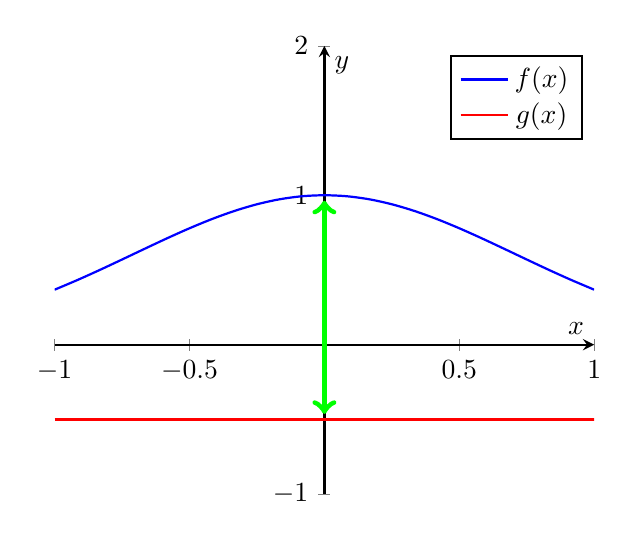
\begin{tikzpicture}
					\begin{axis}[
						xlabel={$x$},ylabel={$y$},
						axis lines=middle,
						thick,
						domain=-1:1,
						ymin=-1,ymax=2
						]
						\addplot[smooth, blue] {e^-(abs(x*x))};
						\addlegendentry{$f(x)$}
						\addplot[smooth, red] {-0.5};
						\addlegendentry{$g(x)$}
						\draw[<->, line width=2pt, color=green, shorten >=2pt, shorten <=2pt] (0,-0.5) -- (0,1);
					\end{axis}
				\end{tikzpicture}
			\end{center}
			\begin{enumerate}[label=\arabic*.]
				\item \label{itm:dist_conv_unif_geq_0} $d(x,y) \geq 0$ per definizione, il valore è sicuramente appartenente a $\intervalclose{0}{+\infty}$, ma $+\infty$ non è un valore accettabile, in quanto la metrica è definita come funzione a valori in $\R$ e $+\infty \notin \R$. D'alto canto, si nota che $X$ è definito come l'insieme delle funzioni continue definite su un intervallo \textbf{chiuso e limitato} a valori in $\R$ ($\cntclass{0}(\intervalclose{a}{b},\R)$). Questa definizione permette di applicare il \fullref{ex:weier_analisi_1} ed avere la certezza che esista $\sup$ finito.
				\item $d(x,y) = 0 \iff x = y$ per definizione, $d_{\cntclass{0}}(f,g) = 0 \iff \sup\limits_{x\in\intervalclose{a}{b}}\abs{g(x)-f(x)} = 0$, cioè se e solo se le due funzioni hanno lo stesso dominio e, per ogni punto di esso, la stessa immagine.
				\item $d(x,y)=d(y,x)$ semplicemente $d_{\infty}(f,g) = \sup\limits_{x\in\intervalclose{a}{b}}\abs{f-g} = \sup\limits_{x\in\intervalclose{a}{b}}\abs{g-f} = d_{\infty}(g,f)$
				\item $d(x,y) \leq d(x,z) + d(z,y)$ dalla disuguaglianza triangolare per $\abs{\;\cdot\;}$ si ottiene
					\[\abs{g(x)-f(x)} \leq \abs{g(x)-h(x)}+\abs{h(x)-f(x)}\]
					Applicando il sup la disuguaglianza resta vera.
			\end{enumerate}
			\begin{note}
				Si sottolinea che queste conclusioni sono valide finché $\intervalclose{a}{b}$ chiuso e limitato, altrimenti non varrebbe più l'\fullref{ex:weier_analisi_1} che è necessario per il punto \ref{itm:dist_conv_unif_geq_0}. % TODO Serve un controesempio
			\end{note}
		\item \label{ex:dist_parigi}\index{Metrica!di Parigi}\index{Distanza!di Parigi}
			$
				\begin{array}{l}
					X=\R^2,\; d \text{ Metrica Euclidea e } P \in X \text{ punto arbitrario }\\
					d_P(x,y)=
					\begin{cases}
						\begin{array}{ll}
							0 & \text{se } x = y\\
							d(x,P) + d(P,y) & \text{se } x \neq y
						\end{array}
					\end{cases}
				\end{array}
			$
			\hfill
			{
				\footnotesize
				\begin{tabular}{c}
					\textbf{Distanza di Parigi}\\[-1ex]
					o\\[-1ex]
					\textbf{Distanza Ferroviaria Francese}
				\end{tabular}
			}
			\begin{enumerate}[label=\arabic*.]
				\item $d(x,y) \geq 0$ per definizione della metrica
				\item $d(x,y) = 0 \iff x = y$ per definizione della metrica
				\item $d(x,y)=d(y,x)$ essendo basata sulla Metrica Euclidea
				\item $d(x,y) \leq d(x,z) + d(z,y)$ essendo basata sulla Metrica Euclidea
			\end{enumerate}
		\item \label{ex:dim_dist_quadratica}\index{Metrica!Quadratica}\index{Distanza!Quadratica}
			$
				\begin{array}{l}
					X=\cntclass{0}(\intervalclose{a}{b},\R)\;a,b\in\R,\;a<b\\
					d_2(f,g) = \sqrt{\int_a^b\left[g(x)-f(x)\right]^2 \integrald{x}}
				\end{array}
			$
			\hfill
			{
				\footnotesize\textbf{Distanza Quadratica}
			}
			\begin{note}
				La metrica viene trattata in \fullref{def:dist_quadratica}
			\end{note}
			\begin{enumerate}[label=\arabic*.]
				\item $d(x,y) \geq 0$ per definizione, essendo integrale di un valore positivo (quadrato) tra estremi ordinati ($a<b$ per ipotesi)
				\item $d(x,y) = 0 \iff x = y$ Per definizione della metrica:
				\[d_2(f,g) = 0 \iff \sqrt{\int_a^b\left[g(x)-f(x)\right]^2 \integrald{x}} = 0\]
				cioè se e solo se le due funzioni hanno lo stesso dominio e, per ogni punto di esso, la stessa immagine.
				\item $d(x,y)=d(y,x)$ semplicemente $d_2(f,g) = \sqrt{\int_a^b\left[g(x)-f(x)\right]^2 \integrald{x}} = \sqrt{\int_a^b\left[f(x)-g(x)\right]^2 \integrald{x}} = d_2(g,f)$
				\item $d(x,y) \leq d(x,z) + d(z,y)$ ... % TODO Spiegare questo punto
			\end{enumerate}
	\end{enumerate}
\end{example}

\begin{definition}[Norma]
	\index{Norma}
	\label{def:norma}
	Dato uno spazio vettoriale $V$ sul campo $\mathbb{K}$, si definisce \textbf{Norma} una funzione $\norm{\cdot}:V \to \R$ con le proprietà:
	\begin{enumerate}
		\item $\norm{x} \geq 0 \quad \forall x\in V$
		\item $\norm{x}=0 \iff x = 0 \quad \forall x\in V$
		\item \label{itm:def_norm_propr_somma} $\norm{x+y} \leq \norm{x}+\norm{y} \quad \forall x,y\in V$
		\item \label{itm:def_norm_propr_lambda} $\norm{\lambda x} = \abs{\lambda} \cdot \norm{x} \quad \forall x\in V,\lambda\in\mathbb{K}$
	\end{enumerate}
	\begin{note}
		La funzione Norma associa dunque ad un vettore di qualsiasi dimensione uno scalare, fornendo (anche) una metrica per ordinare vettori tra loro.
	\end{note}
\end{definition}
\begin{definition}[Spazio Normato]
	\index{Spazio!Normato}
	Uno \textbf{Spazio Normato} è uno spazio vettoriale $V$ sul campo $\mathbb{K}$ \textbf{in cui è definita una norma}.
	\begin{note}
		Nel seguito verranno considerati esclusivamente spazi vettoriali su $\R$ o su $\C$, cioè $\mathbb{K} = \R$ o $\mathbb{K} = \C$
	\end{note}
\end{definition}

\begin{example}[Esempi di Spazi Normati]\leavevmode\vspace*{-\baselineskip}
	\label{ex:sp_norm}
	\begin{enumerate}
		\item $\R$ con $\norm{x} = \abs{x}$
		\item $\C$ con $\norm{x} = \abs{x}$
		\item \label{itm:ex_sp_norm_Rn} $\R^n$ con $\norm{x} = \sqrt{\sum\limits_{i=1}^{n}x_i^2}$
			\begin{note}
				\hypertarget{note:ex_sp_norm_Rn}{}
				Dalla questa definizione di norma segue che $\norm{x}^2 = \sum\limits_{i=1}^{n}x_i^2 = x \cdot x$
			\end{note}
		\item $\cntclass{0}(\intervalclose{0}{1};\R)$ con $\norm{f} = \sup\limits_{x \in \intervalclose{0}{1}} \abs{f(x)}$
			\begin{note}
				Dimostrazione in \fullref{ex:dim_dist_inf}.
			\end{note}
	\end{enumerate}
\end{example}

\begin{proposition}[Metrica Indotta da una Norma]
	\index{Metrica!Indotta da una Norma}
	\index{Distanza!Indotta da una Norma}
	\label{prop:dist_sp_norm}
	Sia $V$ uno spazio normato. Allora $(V,d)$ è uno spazio metrico con la distanza
	\[d(x,y) = \norm{y-x}\]
	ed inoltre la distanza così definita è:
	\begin{enumerate}
		\item Invariante per traslazioni:
			\[\forall x,y,z \in V,\; d(x,y) = d(x+z, y+z)\]
		\item Positivamente omogenea:
			\[\forall x,y \in V \text{ e } \forall \lambda \in \R,\; d(\lambda x, \lambda y) = \abs{\lambda}d(x,y)\]
	\end{enumerate}
	\begin{proof}
		~
		\begin{enumerate}
			\item $d(x,y) = d(x+z, y+z) = \norm{y+z-x-z} = \norm{y-x} = d(x,y)$
			\item Con la proprietà \ref{itm:def_norm_propr_lambda} della \fullref{def:norma}
				\[d(\lambda x, \lambda y) = \norm{\lambda y - \lambda x} = \norm{\lambda (y - x)} = \abs{\lambda} \norm{y - x} = \abs{\lambda}d(x,y)\]
		\end{enumerate}
	\end{proof}
	\begin{note}
		Nel caso in cui $V = \R^n$, la metrica indotta è ovviamente la \textbf{Metrica Euclidea} di \hyperref[ex:dist_eucl]{\fullref*{ex:metriche}}
		% NOTE The \fullref command was not used on purpose to point this link straight to the right part of the aforementioned exercise
		\[d(x,y) = \sqrt{\sum\limits_{i=1}^{n} (y_i-x_i)^2 }\]
	\end{note}
\end{proposition}

\begin{definition}[Metriche Equivalenti]
	\index{Metrica!Equivalente}
	\index{Distanza!Equivalente}
	\label{def:metr_equiv}
	Siano $d_1$ e $d_2$ due distanze sullo stesso insieme $X$.
	\begin{gather*}
		d_1 \text{ e } d_2 \text{ sono \textbf{equivalenti}}\\
		\bydef\\
		\exists c,C \in \intervalopen{0}{+\infty}:\; \forall x,y \in X \quad c \cdot d_1(x,y) \leq d_2 (x,y) \leq C \cdot d_1 (x,y)
	\end{gather*}
	Cioè se è sempre possibile "limitare" una metrica con l'altra (moltiplicata per un opportuno coefficiente). Questo implica che distanze infinite per una metrica devono esserlo anche per l'altra.
	\begin{note}
		Dato uno spazio metrico $(X,d)$, passare dalla distanza $d$ ad un'altra ad essa equivalente è concettualmente analogo ad un cambio di unità di misura. Come esempio si veda \fullref{ex:dist_eqiv}
	\end{note}
\end{definition}
\begin{example}
	La \hyperref[ex:dist_parigi]{Distanza Ferroviaria Francese da \cref*{ex:metriche} (\nameref*{ex:metriche})} e la \hyperref[ex:dist_eucl]{Metrica Euclidea da \cref*{ex:metriche} (\nameref*{ex:metriche})} non sono equivalenti
	% NOTE The \fullref command was not used on purpose to point this link straight to the right part of the aforementioned exercise
	\begin{solution}
		Operando in $\R$ e avendo un $n \in \N$:
		\begin{itemize}[noitemsep]
			\item $P = 0$
			\item $x = n$
			\item $y = n+1$
		\end{itemize}
		Ora, per ogni $n$, si ha $d = 1$, mentre la $d_P = 2n+1$. È dunque impossibile trovare un $C \in \intervalopen{0}{+\infty}$ (quindi \textbf{finito}) tale per cui
		\begin{gather*}
			d_P(x,y) \leq C \cdot d(x,y) \quad \text{con } n \to \infty\\
			2n+1 \leq C \cdot 1 \quad \text{con } n \to \infty
		\end{gather*}
	\end{solution}
\end{example}
\begin{example}
	\label{ex:metr_equiv_R2}
	In $\R^2$, le distanze:
	\begin{align*}
		d_1(x,y) \;\; &= \;\; \abs{y_1 - x_1} + \abs{y_2 - x_2}\\
		d(x,y) \;\; &= \;\; \sqrt{(y_1 - x_1)^2 + (y_2 - x_2)^2}\\
		d_{\cntclass{0}}(x,y) \;\; &= \;\; \max (\abs{y_1 - x_1}, \abs{y_2 - x_2})
	\end{align*}
	sono tutte equivalenti tra di loro.
\end{example}

\begin{definition}[Sfera Aperta]
	\index{Sfera Aperta}
	Sia $(X,d)$ uno spazio metrico e siano $x_0 \in X$, $r > 0$. Si dice \textbf{Sfera} (o \textbf{Bolla}, o ancora \textbf{Palla}) \textbf{Aperta} di centro $x_0$ e raggio $r$ l'insieme:
	\[B(x_0,r)=\brackets{x\in X : d(x,y)<r}\]
\end{definition}
\begin{observation}
	Se $r=0 \implies B(x_0,r)=\emptyset$\\
	Se $r>0 \implies x_0\in B(x_0,r)$
\end{observation}
\begin{example}[Sfere ed Altri Enti]\leavevmode\vspace*{-\baselineskip}
	\begin{itemize}
		\item In $\R$ con $d$, $B(x_0,r)$ è un intervallo simmetrico centrato in $x_0$
		\item In $\R^2$ con $d$, $B(x_0,r)$ è un cerchio con centro in $x_0$
		\item In $\R^3$ con $d$, $B(x_0,r)$ è una sfera con centro in $x_0$
	\end{itemize}
\end{example}
\begin{exercise}
	Descrivere le sfere nelle distanze dell'\fullref{ex:metr_equiv_R2}.
	% TODO soluzione
\end{exercise}

\begin{definition}[Intorno]
	\index{Intorno}
	Sia $(X,d)$ uno spazio metrico e sia $x \in X$. \textbf{Intorno} di $x$ è un qualunque sottoinsieme di $X$ che contenga una sfera aperta contenente $x$
\end{definition}

\begin{definition}[Punti e Spazi Metrici]
	\index{Punto!Interno}
	\index{Punto!Esterno}
	\index{Punto!di Frontiera}
	\index{Punto!Isolato}
	\index{Punto!di Accumulazione}
	\label{def:pti_e_spa_metr}
	Siano $(X,d)$ uno Spazio Metrico, $A \subseteq X$ e $x_0 \in X$:
	\begin{itemize}
		\item \makebox[14em][l]{$x_0$ \textbf{Interno} ad $A$} $\bydef$ \quad $\exists r > 0:\; B(x_0, r) \subseteq A$\newline
			{\footnotesize Cioè è possibile individuare una sfera interamente contenuta in $A$}
		\item \makebox[14em][l]{$x_0$ \textbf{Esterno} ad $A$} $\bydef$ \quad $\exists r > 0:\; B(x_0, r) \subseteq X \setminus A$\newline
			{\footnotesize Cioè è possibile individuare una sfera interamente contenuta in $X$ e NON in $A$}
		\item \makebox[14em][l]{$x_0$ \textbf{di Frontiera} per $A$} $\bydef$ \quad $\forall r > 0,\; B(x_0, r) \nsubseteq A \text{ e } B(x_0, r) \nsubseteq X \setminus A$\newline
			{\footnotesize Cioè, per qualsiasi $r$, la sfera non appartiene completamente né ad $A$, né a $X \setminus A$}
		\item \makebox[14em][l]{$x_0$ \textbf{Isolato} per $A$} $\bydef$ \quad $\exists r > 0:\; B(x_0, r) \cap A = \brackets{x_0}$\newline
			{\footnotesize Cioè è possible trovare un $r$ per cui l'intersezione tra la sfera ed $A$ contiene solo $x_0$\\
			Esempio: $A = \N$, insieme dei numeri naturali, e $r = \frac{1}{2}$}
		\item \makebox[14em][l]{$x_0$ \textbf{di Accumulazione} per $A$} $\bydef$ \quad $\forall r > 0,\; \bigl( B(x_0, r) \cap A \bigr) \setminus \brackets{x_0} \neq \emptyset$\newline
			{\footnotesize Cioè, per qualsiasi $r$, l'intersezione tra la sfera ed $A$ è sempre non vuota (non considerando $x_0$ stesso)}
			\begin{note}
				Si è posto $x_0 \in X$, dunque $x_0$ può essere di Accumulazione per $A$ con $x_0 \notin A$. È sufficiente che $x_0$ sia indefinitamente vicino ai punti di $A$.
			\end{note}
	\end{itemize}
\end{definition}
\begin{example}
	Dato l'insieme $A \subset \R^2$ munito della Distanza Euclidea e rappresentato in figura
	\begin{center}
		\begin{tikzpicture}[scale=0.9]
			\draw plot[smooth, tension=.7] coordinates
				{(-3.5,0.5) (-3,2.5) (-1,3.5) (1.5,3) (4,3.5) (5,2.5) (5,0.5) (2.5,-2) (0,-0.5) (-3,-2) (-3.5,0.5)};
			\node[circle, fill=black, inner sep=1.2pt, label=north east:$R$] at (0,-1.5) {};
			\node[circle, fill=black, inner sep=1.2pt, label=north east:$P$] at (-1.5,1) {};
			\node[circle, fill=black, inner sep=1.2pt, label=east:$Q$] at (5,.5) {};
			\node at (3.5,2.5) {$A$};
		\end{tikzpicture}
	\end{center}
	Si hanno:
	\begin{itemize}[noitemsep]
		\item $P$ Interno
		\item $Q$ di Frontiera
		\item $R$ Esterno
		\item $P$ e $Q$, inoltre, son di Accumulazione per $A$
	\end{itemize}
\end{example}
\begin{definition}[Topologia Spazi Metrici]
	\index{Insieme!Parte Interna}
	\index{Insieme!Frontiera}
	\index{Insieme!Chiusura}
	\label{def:topologia_spa_metri}
	Siano $(X,d)$ uno spazio metrico e $A \subseteq X$. Si definiscono:
	\begin{itemize}
		\item \makebox[11em][l]{\textbf{Parte Interna di} $\boldsymbol{A}$}
			$\bydef \quad \circdot{A} = \brackets{x \in X:\; x \text{ è \textbf{Interno} ad } A}$
		\item \makebox[11em][l]{\textbf{Frontiera di} $\boldsymbol{A}$}
			$\bydef \quad \partial A = \brackets{x \in X:\; x \text{ è \textbf{di Frontiera} per } A}$
		\item \makebox[11em][l]{\textbf{Chiusura di} $\boldsymbol{A}$}
			$\bydef \quad \overline{A} = \brackets{
			x \in X:\; x \brackets{
				\text{
					\small
					\begin{tabular}{c}
						\textbf{Appartiene} ad $A$\\[-.5ex]
						\textit{o}\\
						è \textbf{di Accumulazione} per $A$
					\end{tabular}
					}
				}
			}$
	\end{itemize}
\end{definition}
\begin{example}
	Siano $X = \R$ con $d(x,y)  = \abs{y-x}$, $A = \brackets{1} \cup \intervalclop{2}{3}$, allora:
	\begin{itemize}[noitemsep]
		\item $1$ è un punto isolato per $A$
		\item $5$, ad esempio, è un punto esterno ad $A$
		\item $\overline{A} = \brackets{1} \cup \intervalclose{2}{3}$
		\item $\circdot{A} = \intervalopen{2}{3}$
		\item $\partial A = \brackets{1, 2, 3}$
	\end{itemize}
\end{example}
\begin{example}
	Sia $X = \R$ con $d(x,y)  = \abs{y-x}$\\
	Valgono le uguaglianze $\circdot{\R} = \R$, \quad $\overline{\R} = \R$, \quad $\partial \R = \emptyset$
\end{example}
\begin{proposition}
	\label{prop:chius_sp_metr}
	Siano $(X,d)$ uno spazio metrico, $A \subseteq X$, $A \neq \emptyset$. Allora
	\[\overline{A} = \brackets{x \in A \text{ è \textbf{isolato} per } A} \cup \brackets{x \in A: x \text{ è \textbf{di accumulazione} per } A}\]
	% WARNING Nel secondo elemento dell'unione, sul libro, è riportato x \in X, non x \in A. Non mi sembrava sensato, dunque l'ho cambiato in questo modo.
	\begin{proof}
		Un punto isolato, per definizione, appartiene ad $A$, e rientra quindi automaticamente nella definizione di $\overline{A}$. È dunque necessario dimostrare solo il caso $x_*$ di accumulazione per $A$.\\
		Partiamo dunque dall'ipotesi:
		\begin{align*}
			&x_* \in A \text{ e } x_* \text{ \textbf{non} isolato per } A\\
			\implies &x_* \in A \text{ e \textbf{non} } [ \exists r > 0:\; B(x_*, r) \cap A = \brackets{x_*} ]\\
			\implies &x_* \in A \text{ e } [ \forall r > 0:\; B(x_*, r) \cap A \neq \brackets{x_*} ]
			\intertext{Questo significa che in $B \cap A$ ci son sicuramente altri punti, che poi è come dire}
			\implies &x_* \in A \text{ e } \underbrace{B(x_*, r) \cap A \setminus X \neq \emptyset}_{\mathclap{\text{Definizione di punto di accumulazione}}}
		\end{align*}
	\end{proof}
\end{proposition}
\begin{proposition}
	\label{prop:relaz_sp_metr_1}
	Siano $(X,d)$ uno spazio metrico, $x_0 \in X$ e $A \subseteq X$, $A \neq \emptyset$. Allora valgono le seguenti relazioni
	\begin{enumerate}
		\item $x_0$ \textbf{isolato} per $A \implies x_0 \in A$
		\item $x_0$ \textbf{isolato} per $A \implies
			\begin{cases}
				\begin{array}{c}
					A = \brackets{x_0}\\[-1ex]
					o\\[-1ex]
					\inf\limits_{A \setminus \brackets{x_0}} d(x,x_0) > 0
				\end{array}
			\end{cases}
			$
		\item $x_0$ \textbf{interno} ad $A \implies x_0 \in A$
		\item $x_0$ \textbf{esterno} ad $A \iff \inf\limits_A d(x,x_0) > 0$
		\end{enumerate}
\end{proposition}
\begin{proposition}[Condizione Punti Accumulazione]
	\index{Punto!di Accumulazione!Condizione}
	\label{prop:condiz_punt_accumulaz}
	Siano $(X,d)$ uno spazio metrico, $x_0 \in X$ e $A \subseteq X$, $A \neq \emptyset$. Allora
	\begin{equation*}
		\begin{gathered}
			x_0 \text{ è di \textbf{accumulazione} per } A\\
			\iff\\
			\inf \brackets{d(x,x_0) : x \in A, x \neq x_0} = 0
		\end{gathered}
	\end{equation*}
	Cioè se la "minima distanza" tra $x_0$ ed un altro punto qualsiasi di $A$ è $0$.
\end{proposition}
\begin{proposition}
	\label{prop:relaz_sp_metr_2}
	Siano $(X,d)$ uno spazio metrico, $x_0 \in X$ e $A \subseteq X$, $A \neq \emptyset$. Valgono le seguenti relazioni:
	\begin{enumerate}
		\item $\overline{A} = \brackets{x_0 \in X:\; \inf\limits_{x \in A} d(x, x_0) = 0}$
		\item $\overline{\emptyset} = \emptyset$
		\item $\partial A = \overline{A} \cap \overline{X \setminus A}$
		\item $\circdot{A} \cap \partial A \neq \emptyset$
		\item $\overline{A} = \circdot{A} \cup \partial A$
	\end{enumerate}
\end{proposition}
\begin{exercise}
	Dimostrare nel dettaglio le proposizioni \fullref{prop:chius_sp_metr}, \fullref{prop:relaz_sp_metr_1}, \fullref{prop:condiz_punt_accumulaz}, \fullref{prop:relaz_sp_metr_2}.
	% TODO proofs
\end{exercise}

\begin{definition}[Insieme Aperto]
	\index{Insieme!Aperto}
	\label{def:aperto}
	Siano $(X,d)$ uno spazio metrico e $A\subseteq X$, $A \neq \emptyset$. Si definisce
	\[A\text{ è \textbf{Aperto}} \quad \bydef \quad A=\emptyset\quad\text{oppure}\quad A=\circdot{A}\]
\end{definition}
\begin{definition}[Insieme Chiuso]
	\index{Insieme!Chiuso}
	\label{def:chiuso}
	Siano $(X,d)$ uno spazio metrico e $A\subseteq X$, $A \neq \emptyset$. Si definisce
	\[A\text{ è \textbf{Chiuso}} \quad \bydef \quad A=\emptyset\quad\text{oppure}\quad A=\bar{A}\]
\end{definition}
\begin{observation}
	$A$ \textbf{non chiuso} $\notimplies$ $A$ aperto\\
	$A$ \textbf{non aperto} $\notimplies$ $A$ chiuso
\end{observation}
\begin{example}
	\label{ex:ins_non_ap_non_chius}
	L'insieme $C = \brackets{(x,y) \in \R^2:\; x^2+y^2 \leq 1} \setminus \brackets{(1,0)}$ è né aperto né chiuso.
	\begin{solution}~\newline
		Non è chiuso in quanto la sua frontiera è $\partial C = \brackets{(x,y) \in \R^2:\; x^2+y^2 = 1}$, dunque $(1,0) \in \partial C$, ma per definizione $(1,0) \notin C$\\
		Non è aperto in quanto, scegliendo ad esempio $(1,1) \in C$, è impossibile trovare una sfera $B\bigl( (1,1), r \bigr)$ interamente contenuta in $C$.
	\end{solution}
\end{example}
\begin{exercise}
	\label{ex:ins_aperti_chiusi}
	Dimostrare che in uno spazio metrico $(X,d)$:
	\begin{enumerate}
		\item Ogni sfera di raggio strettamente positivo è un aperto
		\item \label{itm:chiusura_sfera} $\overline{B(x_0,r)} \subseteq \brackets{x \in X:\; d(x,x_0) \leq r}$
		\item $X$ è aperto ed anche chiuso
		\item $\emptyset$ è aperto ed anche chiuso
		\item Sia $A \subseteq X$. Se $A$ è aperto, allora il complementare di $A$ in $X$ è chiuso
		\item Sia $A \subseteq X$. Se $A$ è chiuso, allora il complementare di $A$ in $X$ è aperto
		\item Sia $A \subseteq X$. Allora $\overline{A}$ è chiuso e $\circdot{A}$ è aperto
	\end{enumerate}
	% TODO soluzione
\end{exercise}
\begin{proposition}
	Sia $(X,d)$ lo spazio metrico con la Metrica Discreta (da \hyperref[ex:dist_discr]{\fullref*{ex:metriche}}).\\
	% NOTE The \fullref command was not used on purpose to point this link straight to the right part of the aforementioned exercise
	Allora, preso un $x_0 \in X$ ed un $r > 0$, l'inclusione $\overline{B(x_0,r)} \subseteq \brackets{x \in X:\; d(x,x_0) \leq r}$ è stretta se e soltanto se $r = 1$
\end{proposition}
\begin{exercise}
	Esibire in un opportuno spazio metrico esempi di insiemi né aperti né chiusi.
	% TODO examples
\end{exercise}

\begin{definition}[Diametro Spazio Metrico]
	\index{Diametro}
	Siano $(X,d)$ uno spazio metrico e $A\subseteq X$, $A \neq \emptyset$. Si definisce
	\[\boldsymbol{\diam}(A) \quad = \quad \sup\limits_{\mathclap{x,y \in A}} d(x,y)\]
	Cioè la "distanza massima" tra due suoi qualsiasi elementi.
\end{definition}
\begin{definition}[Spazio Metrico Limitato]
	\index{Spazio!Limitato}
	Siano $(X,d)$ uno spazio metrico e $A\subseteq X$, $A \neq \emptyset$. Allora
	\begin{align*}
		A \text{ è \textbf{Limitato}} \quad &\bydef \quad \diam(A) \text{ è finito}\\
		A \text{ è \textbf{Illimitato}} \quad &\bydef \quad \diam(A) \text{ è infinito}
	\end{align*}
\end{definition}
\begin{note}
	L'insieme vuoto $\emptyset$ ha diametro nullo ed è dunque limitato.
\end{note}
\begin{example}[Diametri e Limitatezza in Spazi Metrici]\leavevmode\vspace*{-\baselineskip}
	\begin{enumerate}
		\item $\R$ con $d(x,y) = \abs{y-x}$ è uno spazio metrico illimitato. Inoltre se $A \subseteq \R$ con $A \neq \emptyset$, allora $\diam(A) = \sup A - \inf A$
		\item $\R$ con $d(x,y) = \frac{\abs{y-x}}{1-\abs{y-x}}$ è uno spazio metrico limitato di diametro $1$ (la distanza massima tra due punti con questa metrica è $1$)
		\item Sia $X$ un insieme con almeno $2$ elementi munito della Metrica Discreta (da \hyperref[ex:dist_discr]{\fullref*{ex:metriche}}) è uno spazio metrico limitato di diametro $1$ % NOTE The \fullref command was not used on purpose to point this link straight to the right part of the aforementioned exercise
		\item $\cntclass{0}(\intervalclose{0}{1}; \R)$ con $d(f,g) = \sup\limits_{\intervalclose{0}{1}} \abs{g(x)-f(x)}$ è uno spazio metrico illimitato utilizzato in \fullref{sect:conv_unif}
	\end{enumerate}
\end{example}
\begin{exercise}
	Siano $(X,d)$ uno spazio metrico e $A,B\subseteq X$. Dimostrare le seguenti implicazioni:
	\begin{enumerate}
		\item $
			\left.
			\mathmakebox[7em][l]{
				\begin{array}{ll}
					A \subseteq B\\
					A \text{ illimitato}
				\end{array}
			}
			\right\} \implies B \text{ illimitato}$
		\item $
			\left.
			\mathmakebox[7em][l]{
				\begin{array}{ll}
				A \subseteq B\\
				B \text{ limitato}
				\end{array}
			}
			\right\} \implies A \text{ limitato}$
		\item $
			\left.
			\mathmakebox[7em][l]{
				\begin{array}{ll}
				A \text{ limitato}\\
				B \text{ limitato}
			\end{array}
			}
			\right\} \implies  A \cup B \text{ limitato}$
	\end{enumerate}
	% TODO soluzione
\end{exercise}
\begin{exercise}
	Dimostrare che in $\R$ le distanze
	\[d(x,y) = \abs{y-x} \quad \text{e} \quad d(x,y) = \frac{\abs{y-x}}{1+\abs{y-x}}\]
	non sono equivalenti.
	\begin{solution}
		Suggerimento: utilizzare la nozione di limitatezza.
		% TODO soluzione
	\end{solution}
\end{exercise}
\begin{exercise}
	\label{ex:sfere_e_limitatezza}
	Dimostrare che in uno spazio metrico $(X,d)$:
	\begin{enumerate}
		\item Se $x_0 \in X$ e $r > 0$, allora $\diam \bigl( B(x_0, r) \bigr) \leq 2r$ (si veda \fullref{ex:diam_sp_metr})
		\item Se $A \subseteq X$ e $x_0 \in A$, allora $A$ è limitato se e solo se esiste un $r>0:\; A \subseteq B(x_0,r)$
	\end{enumerate}
	% TODO soluzione
\end{exercise}
\begin{exercise}
	Sia $X = \R$ con la distanza $d(x,y) = \abs{y-x}$.\\
	Dimostrare che $\diam \bigl( B(0,1) \bigr) = 2$
	% TODO soluzione
\end{exercise}
\begin{exercise}
	\label{ex:diam_sp_metr}
	Sia $X = \intervalclose{0}{2}$ con la distanza $d(x,y) = \abs{y-x}$.\\
	Dimostrare che $\diam \bigl( B(0,1) \bigr) = 1$
	% TODO soluzione
\end{exercise}

\begin{proposition}
	Siano $(X,d)$ uno spazio metrico e $A,B\subseteq X$:
	\[A \subseteq B \implies \diam(A) \leq \diam(B)\]
	\begin{proof}
		Immediata % TODO proof
	\end{proof}
\end{proposition}
\begin{exercise}
	Dimostrare con esempi che:
	\begin{enumerate}
		\item $A \subset B \notimplies \diam(A) < \diam(B)$
		\item $\diam(A) < \diam(B) \notimplies A \subset B$
		\item $\diam(A) \leq \diam(B) \notimplies A \subseteq B$
		\item $\diam(A) = 0 \notimplies A = \emptyset$ % Metrica a lunghezza zero?
	\end{enumerate}
	% TODO soluzione
\end{exercise}
\begin{exercise}
	Esibire in $\R$, $\R^2$ ed in $\cntclass{0}(\intervalclose{0}{1}; \R)$ (con le metriche usuali) esempi di insiemi aperti/chiusi e limitati/illimitati.
\end{exercise}

\begin{definition}[Insieme Finito ed Infinito]
	\index{Insieme!Finito ed Infinito}
	Un insieme si dice \textbf{Finito} se il numero dei suoi elementi è finito.\\
	Un insieme si dice \textbf{Infinito} se non è Finito.
\end{definition}
\begin{observation}
	Con la metrica Euclidea, ogni insieme finito è limitato e ogni insieme illimitato è infinito. Non valgono i viceversa.
\end{observation}

\newpage
\section{Successioni e Completezza}\label{sect:succ_compl}
\begin{definition}[Successione]
	\index{Successione}
	\label{def:succ}
	Sia $X$ un insieme non vuoto. \textbf{Successione} in $X$ è una funzione $x: \N \to X$.
	\begin{note}
		Altre possibili notazioni per le successioni sono: $x_n$, $(x_n)_{n \in \N}$ e $\brackets{x_n:\; n \in \N}$.\\
		Con $x_n$ si indica spesso anche \textbf{il valore assunto} dalla successione $x$ al suo $n$\textit{-esimo} elemento.
	\end{note}
\end{definition}
\begin{definition}[Successione Limitata e Illimtata]
	\index{Successione!Limitata e Illimtata}
	Una successione $x: \N \to X$ di elementi di uno spazio metrico $(X,d)$ si dice \textbf{Limitata} se il suo codominio $x(\N)$ è limitato.\\
	Una successione è \textbf{Illimitata} se il suo codominio $x(\N)$ è illimitato.
\end{definition}
\begin{definition}[Limite per Successioni] % TODO la definizione di limite per successioni va modificata per offrire la classica distanza delta-epsilon
	\index{Limite!per Successioni}
	\index{Successione!Convergente}
	\label{def:lim_succ}
	Data una successione $x: \N \to X$ di elementi di uno spazio metrico $(X,d)$ e dato $x_\infty \in X$
	\begin{equation}
		\label{eq:lim_succ}
		\lim\limits_{n \to +\infty} = x_\infty \quad \bydef \quad \lim\limits_{n \to +\infty} d(x_n,x_\infty) = 0
	\end{equation}
	Se $\lim\limits_{n \to +\infty} = x_\infty$, allora la successione $x_n$ è \textbf{Convergente} a $x_\infty$. Si può scrivere: $x_n \to x_\infty$ per $n \to \infty$.

	Cioè la convergenza della successione $x: \N \to X$ a $x_\infty$ equivale alla convergenza a $0$ della successione di numeri reali $\brackets{d(x_n,x_\infty):\; n \in \N}$
	\begin{note}
		Essendo posto $x_\infty \in X$, $x_\infty$ deve appartenere allo spazio metrico. In caso alternativo il limite non esiste.
	\end{note}
	\begin{note}
		Questa definizione è \textit{implicita}, cioè non porta a nessun metodo \textit{costruttivo} per calcolare il limite di una successione. La definizione di limite permette soltanto di verificare se una nota quantità è limite della successione data o meno.
	\end{note}
\end{definition}
\begin{proposition}
	\label{prop:succ_conv_lim}
	Data la successione $x: \N \to X$ di elementi dello spazio metrico $(X,d)$ e dato $x_\infty\in X$:
	\[\lim\limits_{n \to+\infty}x_n = x_\infty \quad \iff \quad \forall\varepsilon > 0 \quad \exists\nu\in\N:\; \forall n>\nu \text{ vale } d(x_n,x_\infty)<\varepsilon\]
	\vspace*{-\baselineskip}
	\begin{note}
		Questa definizione coincide con la definizione di Limite di Successione di numeri reali data nel corso di Analisi 1 se $X = \R$ e $d(x, y) = \abs{y - x}$.
	\end{note}
	\begin{proof}
		L'argomento del limite al secondo membro di \cref{eq:lim_succ} è una una successione del tipo
		\[y_n = d(x_n,x_\infty)\]
		Inoltre è successione di numeri reali, per \fullref{def:sp_metrico} infatti $d: X \times X \to \R$. Applicando alla $y_n$ la definizione di Limite di Successione di numeri reali (dal corso di Analisi 1) si giunge alla tesi.
	\end{proof}
\end{proposition}
\begin{theorem}[di Unicità del Limite per Successioni]
	\index{Teorema!di Unicità del Limite per Successioni}
	\index{Unicità!del Limite per Successioni}
	Sia $(X,d)$ uno spazio metrico e siano $x_\infty, x^\infty$ elementi di $X$ e $x: \N \to X$ una successione in $X$.
	\begin{equation*}
		\left.
		\begin{array}{l}
			\lim\limits_{n \to +\infty} x_n = x_\infty\\
			\lim\limits_{n \to +\infty} x_n = x^\infty\\
		\end{array}
		\quad\right\}
		\implies x_\infty = x^\infty
	\end{equation*}
	\begin{proof}
		Per ogni $n \in \N$, per la proprietà 4 da \fullref{def:sp_metrico}
		\[d(x_\infty, x^\infty) \leq d(x_\infty, x_n) + d(x_n, x^\infty)\]
		Passando al $\lim$ per $n \to +\infty$
		\[
			\underbrace{\lim\limits_{n \to +\infty}d(x_\infty, x^\infty)}_{\begin{tabular}{c}$\geq 0$\\{\small Per def. distanza}\end{tabular}}
			\leq
			\underbrace{\lim\limits_{n \to +\infty}d(x_\infty, x_n)}_{\begin{tabular}{c}$\leq \varepsilon$\\{\small Per def. lim succ.}\end{tabular}}
			+
			\underbrace{\lim\limits_{n \to +\infty}d(n, x^\infty)}_{\begin{tabular}{c}$\leq \varepsilon$\\{\small Per def. lim succ.}\end{tabular}}
			\leq 2 \varepsilon
		\]
		Dovendo essere questa forma valida $\forall \varepsilon > 0$, si concludere che non può esser altro che
		\[\lim\limits_{n \to +\infty}d(x_\infty, x^\infty) = 0\]
		Che, per la proprietà 2 da \fullref{def:sp_metrico}, significa
		\[x_\infty = x^\infty\]
	\end{proof}
\end{theorem}
\begin{proposition}
	\label{prop:succ_conv_se_comp_conv}
	Sia $p \in \N,\; p \geq 2$. In $\R^p$, con $d(x,y) = \norm{y-x}$, una successione $x: \N \to X$ converge a $x_\infty$ se e solo se le $p$ successioni delle componenti convergono alle rispettive componenti di $x_\infty$.
	\begin{proof}
		Applicare la \fullref{def:lim_succ} ricordando che
		\[\abs{y_i} \leq \norm{y} \leq \abs{\sum\limits_{i = 1}^p \abs{y_i}} \qquad \forall y \in \R^p \text{ e per } i = 1,\:\dotsc\:,p\]
		% TODO actual proof
	\end{proof}
\end{proposition}
\begin{exercise}
	Esibire un esempio di successione in $\R^2$ convergente a $(1,1)$ con le distanze introdotte ai punti 3 e 4 dell'\fullref{ex:metriche}.
	% TODO soluzione
\end{exercise}
\begin{exercise}
	Esibire un esempio di successione in $\C$ convergente a $1+i$ con la distanza $d(z,w) = \abs{w-z}$.
	% TODO soluzione
\end{exercise}
\begin{proposition}[Caratterizzazione dei Punti di Accumulazione]
	\index{Caratterizzazione Punti di Accumulazione}
	\label{prop:caratteriz_pti_accumul}
	Siano $(X,d)$ uno spazio metrico, $A \subseteq X$ e $x_* \in X$. Allora
	\[
		x_* \text{ \textbf{di Accumulazione} per } A
		\quad \iff \quad
		\begin{tabular}{c}
			esiste una \textbf{successione} di elementi di $A$,\\[-.5ex]
			diversi da $x_*$, \textbf{convergente} a $x_*$
		\end{tabular}
	\]
	\begin{note}
		La puntualizzazione "diversi da $x_*$" specifica che la successione costante $x_n = x_*$ non è ammissibile.
	\end{note}
	\begin{proof}~
		\begin{itemize}
			\item[$\implies$] Grazie alla \fullref{prop:condiz_punt_accumulaz}
				\begin{align*}
					&x_* \text{ è di accumulazione per } A\\
					\implies &\inf \brackets{d(x,x_*):\; x \in A, x \neq x_0} = 0
					\shortintertext{Che equivale a scrivere}
					\implies &\forall \varepsilon > 0\; \exists x_\varepsilon \in A:\; x_\varepsilon \neq x_* \text{ e } d(x_\varepsilon, x_*) < \varepsilon
					\shortintertext{Quindi si può scegliere arbitrariamente un $\varepsilon = \frac{1}{n}$, ponendo $n \neq 0$ ed arrivare a}
					\implies &\forall n \in \N \setminus \brackets{0},\: \exists x_n \in A:\; x_n \neq x_* \text{ e } d(x_n,x_*) < \frac{1}{n}
				\end{align*}
				La successione delle distanze è convergente a $0$ per $n \to +\infty$, quindi con la \fullref{def:lim_succ} si può concludere che la successione $x_n$ converge a $x_*$
			\item[$\impliedby$] Dalla \fullref{def:lim_succ}
				\[\forall\varepsilon > 0 \quad \exists\nu\in\N:\; \forall n>\nu \quad x_n \in A,\: x_n \neq x_*, \quad d(x_n,x_*)<\varepsilon\]
				Ma se $d(x_n,x_*)<\varepsilon$, allora si può anche scrivere $x_n \in B(x_*, \varepsilon)$, quindi sicuramente
				\begin{align*}
					\implies & \forall\varepsilon > 0 \quad B(x_*, \varepsilon) \cap A \setminus \brackets{x_*} \neq \emptyset\\
					\intertext{Dunque stando alla \fullref{def:pti_e_spa_metr}}
					\implies & x_* \text{ è di accumulazione per } A
				\end{align*}
		\end{itemize}
	\end{proof}
\end{proposition}
\begin{corollary}
	\label{coro:succ_conv_sse_x_in_chius_A}
	Siano $(X,d)$ uno Spazio Metrico, $A \subseteq X$ e $x_* \in X$. Allora:
	\[
		x_* \in \boldsymbol{\overline{A}}
		\quad \iff \quad
		\begin{tabular}{c}
			esiste una \textbf{successione} di elementi di $A$,\\[-.5ex]
			diversi da $x_*$, \textbf{convergente} a $x_*$
		\end{tabular}
	\]
	\begin{proof}~
		\begin{itemize}
			\item[$\implies$] Direttamente dalla \fullref{def:topologia_spa_metri}:
				\begin{itemize}
					\item Se $x_* \in A$\newline
						È sufficiente scegliere $x_n = x_*$, successione costante, dunque
						\[\lim\limits_{n \to +\infty} x_n = \lim\limits_{n \to +\infty} x_* = x_*\]
					\item Se $x_*$ di accumulazione per $A$\newline
						Per \fullref{def:topologia_spa_metri} e grazie alla \fullref{prop:caratteriz_pti_accumul} si giunge direttamente alla tesi.
				\end{itemize}
			\item[$\impliedby$] Per \fullref{def:topologia_spa_metri} e grazie alla \fullref{prop:caratteriz_pti_accumul} si giunge direttamente alla tesi.
		\end{itemize}
	\end{proof}
\end{corollary}

\begin{definition}[Successione di Cauchy]
	\index{Successione!di Cauchy}
	\index{Condizione!di Cauchy per Successioni}
	\label{def:succ_cau}
	Sia $(X,d)$ uno spazio metrico e $x: \N \to X$ una successione d in $X$.
	\begin{gather*}
		x:\N \to X \text{ è \textbf{di Cauchy}}\\
		\bydef\\
		\forall \varepsilon > 0\quad \exists \nu \in \N:\; \forall n,m > \nu \text{ vale } d(x_n, x_m) < \varepsilon
	\end{gather*}
	Cioè se la distanza tra due punti qualsiasi della successione, presi dopo un certo valore $\nu$, è minore di un $\varepsilon$ piccolo a piacere.
	\begin{note}
		La seconda riga della definizione è nota come \textbf{Condizione di Cauchy.}
	\end{note}
	\begin{note}
		Questa definizione, differentemente dalla \fullref{def:lim_succ}, è \textit{esplicita} e \textit{intrinseca}: dipende esclusivamente dalla successione e dalla distanza definita.
	\end{note}
\end{definition}
\begin{proposition}
	\label{prop:se_succ_conv_allora_cau}
	Sia $(X,d)$ uno spazio metrico.
	\[x: \N \to X \text{ è \textbf{Convergente}} \quad \implies \quad x:\N \to X \text{ è \textbf{di Cauchy}}\]
	\begin{proof}
		Sia $x: \N \to X$ convergente a $x_\infty$. Allora
		\[\lim\limits_{n \to +\infty} x_n \bydef \forall\varepsilon > 0 \quad \exists\nu\in\N:\; \forall n > \nu \quad d(x_n,x_\infty)<\varepsilon\]
		Prendendo dunque due elementi qualsiasi $n$ e $m$ con $n,m > \nu$, la distanza di ognuno di essi da $x_\infty$ dovrà essere $<\varepsilon$. Applicando la proprietà 4 da \fullref{def:sp_metrico}, otteniamo
		\[d(x_n,x_m) \leq \left[ d(x_n,x_\infty)+d(x_m,x_\infty) \right] < 2\varepsilon\]
		Quindi
		\[\forall\varepsilon > 0 \quad \exists\nu\in\N:\; \forall n,m > \nu \quad d(x_n,x_m) \leq \left[ d(x_n,x_\infty)+d(x_m,x_\infty) \right] < 2\varepsilon\]
		Cioè ci si è ricondotti alla definizione della Condizione di Cauchy
	\end{proof}
\end{proposition}

\begin{definition}[Spazio Metrico Completo]
	\index{Spazio!Completo}
	\label{def:completo}
	Uno Spazio Metrico $(X,d)$ si dice \textbf{Completo} se e solo se \textbf{ogni successione di Cauchy in $X$ ammette limite in $X$ stesso}.
\end{definition}
\begin{example}[Esempi di Spazi Metrici Completi e non]\leavevmode\vspace*{-\baselineskip}
	\label{ex:sp_metr_compl_e_non}
	\begin{enumerate}
		\item $\R$ con $d(x,y) = \abs{y - x}$ è uno spazio metrico completo
		\item $\mathbb{Q}$ con $d(x,y) = \abs{y - x}$ è uno spazio metrico \textit{non} completo
		\item $\R^n$ con $d(x,y) = \norm{y - x}$ è uno spazio metrico completo.
			\begin{note}
				Altre distanze che rendono $\R^n$ uno spazio metrico completo sono, ad esempio
				\begin{itemize}[nolistsep]
					\item $d(x,y) = \max\limits_{i=1,\:\dotsc\:,n} \abs{y_i - x_i}$
					\item $d(x,y) = \left( \sum\limits_{i=1}^{n} \abs{y_i - x_i}^\alpha \right)^{\frac{1}{\alpha}}$ con $\alpha \in \intervalclop{1}{+\infty}$
				\end{itemize}
			\end{note}
		\item $\intervalopen{0}{1}$ con $d(x,y) = \abs{y - x}$ è uno spazio metrico \textit{non} completo.
			\begin{proof}
				La successione $\brackets{\frac{1}{n}:\; n \in \N, n \neq 0}$ è di Cauchy ma non ammette limite in $\intervalopen{0}{1}$
			\end{proof}
		\item Sia $X$ un insieme con almeno 2 elementi, munito della metrica discreta
			\[d(x,y)=
			\begin{cases}
				\begin{matrix}
					0&&x=y\\
					1&&x \ne y
				\end{matrix}
			\end{cases}\]
			$X$ è uno spazio metrico completo in cui le uniche successioni convergenti son le successioni \textbf{definitivamente costanti} (cioè costanti da un certo indice in poi).
		\item $\cntclass{0}(\intervalclose{0}{1}; \R)$ è uno spazio metrico completo con la distanza
			\[d(f,g) = \sup\limits_{\intervalclose{0}{1}}\abs{g(x) - f(x)}\]
			Vedasi \fullref{prop:compat_allora_C0_dC0_sp_metr_compl} per la dimostrazione.
		\item $\cntclass{0}(\intervalclose{0}{1}; \R)$ è uno spazio metrico \textit{non} completo con la distanza
			\[d(f,g) = \sqrt{\int_0^1 \left[ g(x) - f(x) \right]^2 \integrald{x}}\]
			Vedasi \fullref{prop:dist_quad_sp_metr_non_compl} per la dimostrazione.
		\item L'insieme $\C$ dei numeri complessi è uno spazio metrico completo con la distanza $d(z,w) = \abs{w-z}$
	\end{enumerate}
\end{example}
\begin{exercise}
	Esibire una successione di Cauchy di numeri razionali non convergente in $\mathbb{Q}$.
	\begin{solution}
		La successione
		\[x_n = \left( 1+ \frac{1}{n} \right)^n\]
		Converge a $\lim\limits_{n \to +\infty} x_n = e \notin \mathbb{Q}$
	\end{solution}
\end{exercise}
\begin{proposition}
	\label{prop:subset_compl_e_compl}
	Siano $(X,d)$ uno spazio metrico \textbf{completo} e $C \subseteq X$ un sottoinsieme \textbf{chiuso} di $X$. Allora $\boldsymbol{(C,d_{|C})}$ \textbf{è sottospazio metrico completo}, con $d_{|C}$ da \fullref{def:metr_indotta}.
	\begin{proof}
		Essendo $C$ chiuso, per \fullref{def:chiuso}:
		\[C = \overline{C} \implies \forall x_* \in C,\; x_* \in \overline{C}\]
		Si può dunque applicare il \fullref{coro:succ_conv_sse_x_in_chius_A} e concludere che
		\[\forall x_* \in C \text{ esiste un successione di elementi di $C$ convergenti a $x_*$}\]
		Questo permette di individuare tante successioni $x_i$ quanti sono gli elementi di $C$ e, grazie alla \fullref{prop:se_succ_conv_allora_cau}, si sa che ognuna di queste successioni è di Cauchy.\\
		Si giunge dunque alla \fullref{def:completo}
	\end{proof}
	\begin{note}
		\hypertarget{note:subset_compl_e_compl}{}
		La chiusura di $C$ è fondamentale perché diversamente non sarebbe applicabile il \fullref{coro:succ_conv_sse_x_in_chius_A} e dunque non si avrebbe certezza sulla convergenza in $C$ delle successioni.
	\end{note}
\end{proposition}
\begin{proposition}
	\label{prop:se_cau_allora_lim}
	Sia $(X,d)$ uno spazio metrico. Data la successione $x: \N \to X$ \textbf{di Cauchy}:
	\[x: \N \to X \text{\textbf{ di Cauchy}} \quad \implies \quad x: \N \to X \text{ \textbf{Limitata}}\]
	\begin{proof}
		\begin{equation*}
			\begin{gathered}
				x: \N \to X \text{ di Cauchy}\\
				\bydef\\
				\forall \varepsilon > 0\quad \exists \nu \in \N:\; \forall n,m > \nu \text{ vale } d(x_n, x_m) < \varepsilon
			\end{gathered}
		\end{equation*}
		La dimostrazione prevede di dividere in due "parti" la successione
		\begin{enumerate}
			\item Per la definizione di cui sopra è sicuramente possibile individuare un certo $\overline{\nu}$ per cui
				\[\exists \overline{\nu}:\; \forall n > \overline{\nu} \quad d(x_n, x_{\overline{\nu}}) < 1 \qquad \text{(1 è scelto arbitrariamente)}\]
				In tal modo è stata esplicitata la limitatezza di $x$ \textit{da $\overline{\nu}$ in poi}.
			\item Si ponga invece $K = \max\limits_{n=0,\: \dotsc \:, \overline{\nu}-1} d(x_n, x_{\overline{\nu}})$, cioè $K$ è la massima tra tutte le distanze $d(x_n, x_{\overline{\nu}})$ con $n < \overline{\nu}$.\\
				Essendo $n < \overline{\nu}$, $n$ è sicuramente finito, per cui anche $K$ sarà finito. Infatti, avendo un numero finito $n$ di valori $x_n$ assunti dalla successione, anche il massimo di tali valori (cioè $K$) sarà finito.\\
				In questo modo si è trovato un valore $K$ che limita la $x$ \textit{prima di} $\overline{\nu}$.
		\end{enumerate}
		Quindi, concludendo, sicuramente
		\[\forall n \in \N \quad d(x_n, x_{\overline{\nu}}) < \max \brackets{K, 1}\]
		Cioè la successione è limitata.
	\end{proof}
\end{proposition}
\begin{exercise}
	\label{ex:succ_lim_non_cau}
	Definire in un opportuno spazio metrico una successione limitata non di Cauchy.
	\begin{solution}
		In $(\N,d)$ la successione $x(n) = (-1)^n$.
	\end{solution}
\end{exercise}
\begin{corollary}
	Sia $(X,d)$ uno spazio metrico. Data la successione $x: \N \to X$:
	\[x \text{ \textbf{Convergente}} \quad \implies \quad x \text{ \textbf{Limitata}}\]
	\begin{proof}
		Grazie alla \fullref{prop:se_succ_conv_allora_cau} ed alla \fullref{prop:se_cau_allora_lim}
		\[\text{convergente } \implies \text{ di Cauchy } \implies \text{ limitata}\]
	\end{proof}
\end{corollary}
\begin{exercise}
	Definire in un opportuno spazio metrico una successione limitata non convergente.
	\begin{solution}
		Come da \fullref{ex:succ_lim_non_cau} % TODO magari un'altra successione qui
	\end{solution}
\end{exercise}
\begin{exercise}
	Siano $(X,d)$ uno spazio metrico completo, $A \subseteq X$ chiuso e non vuoto. Allora, detta $d_{|A}$ la restrizione di $d$ ad $A$, $(A,d_{|A})$ è uno spazio metrico completo.\\
	È indispensabile l'ipotesi "\textit{$A$ chiuso}"?
	\begin{solution}
		Vedere \hyperlink{note:subset_compl_e_compl}{\notestyle{} alla \fullref*{prop:subset_compl_e_compl}}.
	\end{solution}
\end{exercise}
\begin{exercise}
	Dimostrare che ogni sottosuccessione di una successione di Cauchy è a sua volta una successione di Cauchy.
	% TODO soluzione
\end{exercise}
\begin{exercise}
	\label{ex:sottsucc_conv_succ_conv}
	Dimostrare che se una successione ammette una sottosuccessione convergente, allora l'intera successione è convergente.
	% TODO soluzione
\end{exercise}

\subsection{Insiemi Connessi}
Concettualmente, un insieme è connesso se è \textit{un pezzo solo}. Per dare una definizione formale conviene prima caratterizzare gli insiemi formati \textit{da più pezzi} e poi definire come connessi quelli \textit{non} formati \textit{da più pezzi}.
\begin{definition}[Insiemi Separati]
	\index{Insieme!Separato}
	Siano $(X,d)$ uno spazio metrico, $A \subseteq X$ e $B \subseteq X$
	\[A \text{ e } B \text{ sono \textbf{Separati}} \quad \bydef \quad \overline{A} \cap B = \emptyset \text{ e } A \cap \overline{B} = \emptyset\]
\end{definition}
\begin{definition}[Insiemi Connessi e Sconnessi]
	\index{Insieme!Connesso e Sconnesso}
	\label{def:connesso}
	Un insieme è \textbf{Sconnesso} se e solo se è \textbf{unione} di due insiemi \textbf{separati}.\\
	Un insieme è \textbf{Connesso} se e solo se \textbf{non è Sconnesso}.
	\begin{note}
		In uno spazio metrico un insieme è alternativamente Connesso o Sconnesso e deve sicuramente essere di un tipo o dell'altro. Questa divisione binaria non è applicabile alla classificazione Aperto/Chiuso, in quanto un insieme può anche essere né aperto né chiuso, vedasi \fullref{ex:ins_non_ap_non_chius}.
	\end{note}
\end{definition}
\begin{example}
	In $\R$ con l'usuale distanza Euclidea:
	\begin{enumerate}
		\item $\intervalclose{0}{1}$ e $\intervalopcl{1}{2}$ non sono separati
		\item $\intervalclop{0}{1}$ e $\intervalopcl{1}{2}$ sono separati
		\item $\brackets{0} \cup \intervalclose{1}{2}$ è sconnesso
		\item $\R$ è connesso
	\end{enumerate}
\end{example}
\begin{exercise}
	Dimostrare che gli insiemi $\N$, $\mathbb{Z}$ e $\mathbb{Q}$ sono sottoinsiemi sconnessi di $\R$ con la distanza Euclidea.
	% TODO soluzione
\end{exercise}
\begin{exercise}
	Dimostrare che se due insiemi sono separati, allora sono disgiunti (cioè $A \cap B = \emptyset$). Esibire un controesempio all'implicazione inversa.
	% TODO soluzione
\end{exercise}
\begin{exercise}
	Esibire esempi di insiemi:
	\begin{enumerate}
		\item connessi/sconnessi ed aperti/chiusi
		\item connessi/sconnessi e limitati/illimitati
	\end{enumerate}
	% TODO soluzione
\end{exercise}

\begin{proposition}
	\label{prop:in_Rn_connesso_sse_intervallo}
	In $\R$ con la metrica Euclidea, sia $A \subseteq \R$.
	\[A \text{ è \textbf{Connesso}} \quad \iff \quad A \text{ è un \textbf{Intervallo}}\]
	\begin{proof}
		Omessa.
	\end{proof}
\end{proposition}
\begin{proposition}[Poligonale Congiungente due Punti]
	\index{Poligonale}
	\label{prop:polig_in_aperto_connesso}
	In $\R^n$ con la distanza Euclidea, sia $A$ un \textbf{aperto connesso}. Allora, comunque scelti $x$ e $y$ in $A$, esiste una \textbf{poligonale} interamente contenuta in $A$ con i lati paralleli agli assi e congiungente $x$ a $y$.
	% TODO disegno
	\begin{proof}
		Omessa.
	\end{proof}
\end{proposition}
\begin{exercise}
	Mostrare con un esempio che nella \fullref{prop:polig_in_aperto_connesso} l'ipotesi "\textit{$A$ aperto}" è essenziale.
	\begin{solution}
		Dato lo spazio metrico $(\R^2,d)$, tutti i punti del sottoinsieme $\brackets{x \in \R^2:\;x^2 + y^2 = 1}$ sono di frontiera, dunque non è un aperto. È impossibile individuare una poligonale che colleghi due qualsiasi punti della circonferenza in quanto, appunto, circonferenza.
	\end{solution}
\end{exercise}

\subsection{Insiemi Compatti}
\begin{definition}[Insieme Compatto]
	\index{Insieme!Compatto}
	\label{def:compatto}
	Siano $(X,d)$ uno spazio metrico e $A \subseteq X$. $A$ è \textbf{Compatto} se e solo se \textbf{ogni successione di elementi di $A$ ammette una sottosuccessione avente limite in $A$}.
	\begin{note}
		Questa è la definizione di \textbf{Compattezza per Successioni}, in spazi più generali può essere necessario utilizzare una definizione più debole che, nel caso degli spazi metrici, coincide con la precedente.
	\end{note}
\end{definition}
\begin{proposition}~
	\label{prop:compat_chius_lim}
	\vspace*{-\baselineskip}
	\begin{note}
		Questo teorema è anche noto come \textit{Teorema di Heine-Borel}
	\end{note}
	Siano $(X,d)$ uno spazio metrico e $A \subseteq X$
	\[A \text{ \textbf{Compatto}} \quad \implies \quad A \text{ \textbf{Chiuso} e \textbf{Limitato}}\]
	\begin{proof}
		Per assurdo negando una per una le conclusioni.
		\begin{itemize}
			\item $A$ non è chiuso
				\begin{align*}
					&A \text{ non è chiuso}\\
					\implies &A \neq \overline{A}\\
					\implies &A \subset \overline{A}\\
					\implies &\exists x_0 \in \overline{A},\; x_0 \notin A\\
					\shortintertext{Dunque, per \fullref{def:topologia_spa_metri}, si deve concludere che}
					\implies &\exists x_0 \text{ di accumulazione per } A,\; x_0 \notin A\\
					\shortintertext{Quindi dalla \fullref{prop:caratteriz_pti_accumul}}
					\implies &x:\; \N \to X \text{ con }
						\begin{cases}
							x_n \in A\; \forall n\\
							\lim\limits_{n \to +\infty} x_n = x_0, x_0 \notin A
						\end{cases}\\
					\shortintertext{Cioè abbiamo ottenuto una successione non convergente in $A$, dunque negando l'ipotesi}
					\implies &A \text{ non è compatto - \textit{Assurdo}}
				\end{align*}
			\item $A$ non è limitato
				\begin{align*}
					&A \text{ non è limitato}\\
					\implies &\sup \brackets{d(x,y): x,y \in A} = + \infty\\
					\shortintertext{Fissato dunque un $x_0 \in A$, continuerò ad aver distanza infinita, in quanto $A$ non limitato per ipotesi.}
					\implies &\sup\limits_{x \in A} d(x,x_0) = + \infty\\
					\implies &\forall n \in \N,\; \exists x_n \in A:\; d(x_n, x_0) > n
					\shortintertext{Dunque qualsiasi sottosuccessione di $x:\; \N \to X$ è illimitata}
					\implies &x:\; \N \to X \text{ è una successione in $A$ senza sottosuccessioni convergenti}\\
					\implies &A \text{ non è compatto - \textit{Assurdo}}
				\end{align*}
		\end{itemize}
	\end{proof}
\end{proposition}
\begin{proposition}
	\label{prop:compat_chius_lim_Rn}
	In $\R^n$ con l'usuale metrica Euclidea, sia $A \subseteq \R^n$. Allora:
	\[A \text{ è \textbf{Compatto}} \quad \iff \quad A \text{ è \textbf{Chiuso} e \textbf{Limitato}}\]
	\begin{proof}
		Omessa a lezione.\\
		\cbstart
		Nel caso $n = 1$, segue dalle (note) proprietà di $\R$. Nel caso $n > 1$, si veda \fullref{ex:compat_chius_lim_Rn}.
		\cbend
	\end{proof}
\end{proposition}
\begin{note}
	La \fullref{prop:compat_chius_lim} vale in ogni spazio metrico, mentre la \fullref{prop:compat_chius_lim_Rn} solo in $A \subseteq \R^n$
\end{note}
\cbstart
\begin{exercise}
	\label{ex:compat_chius_lim_Rn}
	Completare la dimostrazione della \fullref{prop:compat_chius_lim_Rn}.\\
	Suggerimento: utilizzare il caso $n = 1$ e la e la \fullref{prop:succ_conv_se_comp_conv}
\end{exercise}
\begin{exercise}
	Confrontare la dimostrazione della \fullref{prop:compat_chius_lim_Rn} con \fullref{ex:ins_chius_lim_non_compl}
\end{exercise}
\cbend
\begin{exercise}
	In uno spazio metrico, esibire esempi di insiemi connessi/sconnessi e compatti/non compatti.
	% TODO solution
\end{exercise}
\begin{exercise}
	In $\R$ con la distanza Euclidea, esibire esempi di insiemi che siano intervalli/non intervalli compatti/non compatti
	% TODO solution
\end{exercise}
\begin{exercise}
	\label{ex:unione_compatti}
	Sia $(X,d)$ uno spazio metrico. Siano $K_1$ e $K_2$ due sottoinsiemi \textbf{Compatti} di $X$. Allora $K_1 \cup K_2$ è \textbf{Compatto}.
	\begin{solution}
		Posto $K = K_1 \cup K_2$, per definizione di \textbf{unione}, ogni elemento di $K$ è in $K_1$ o $K_2$.\\
		Visto che, per ipotesi, $K_1$ e $K_2$ sono compatti, sappiamo che ogni successione in uno dei due avrà una sottosuccessione convergente nello stesso insieme. A questo punto possiamo concludere che ogni successione in $K$ ammetterà una sottosuccessione convergente ad un elemento $x_\infty \in K_1$ oppure $x_\infty \in K_2 \implies x_\infty \in K$
	\end{solution}
\end{exercise}

\begin{proposition}
	\label{prop:X_compat_allora_X_compl}
	Sia $(X,d)$ uno spazio metrico. Allora
	\[X \text{ è \textbf{Compatto}} \quad \implies \quad X \text{ è \textbf{Completo}}\]
	\begin{proof}
		Sia $x: \N \to X$ una successione di Cauchy di elementi di $X$.\\
		$X$ è compatto quindi, per definizione, esiste una sottosuccessione convergente ad un $x_\infty \in X$. Ciò implica, grazie all'\fullref{ex:sottsucc_conv_succ_conv}, che l'intera successione converga a $x_\infty$, dunque $X$ è completo.
	\end{proof}
\end{proposition}

\begin{observation}
	Sia $X$ un insieme munito di due \reffull{def:metr_equiv} $d_1$ e $d_2$. Allora \textit{ciò che vale in $(X, d_1)$, vale in $(X, d_2)$}\\
	Il seguente esercizio rende rigorosa questa affermazione.
\end{observation}
\begin{exercise}
	\label{ex:dist_eqiv}
	Sia $X$ un insieme munito delle due distanze $d_1$ e $d_2$ tra loro equivalenti. Se un insieme è Aperto (Chiuso, Compatto, Connesso, Limitato) \textbf{in} $\boldsymbol{(X,d_1)}$, allora \textbf{lo è anche in} $\boldsymbol{(X,d_2)}$.\\
	Inoltre, \textbf{se} $\boldsymbol{\lim\limits_{n \to +\infty} x_n = x_\infty}$ \textbf{in} $\boldsymbol{(X,d_1)}$, allora $\boldsymbol{\lim\limits_{n \to +\infty} x_n = x_\infty}$ \textbf{anche in in} $\boldsymbol{(X,d_2)}$
	% TODO solution
\end{exercise}
\begin{example}
	Sia $(X,d)$ lo spazio $\R^n$ munito della distanza Euclidea. Sia $d_p$ come in \hyperref[ex:dist_parigi]{\fullref*{ex:metriche}} con $p \in \R^n$\\
	% NOTE The \fullref command was not used on purpose to point this link straight to the right part of the aforementioned exercise	
	È interessante notare che in $(X,d)$, $d_p$ stessa non è continua e quindi gli insiemi aperti (chiusi) rispetto a $d_p$, possono non essere aperti (chiusi) rispetto alla distanza Euclidea. Di conseguenza son proprietà diverse nei due spazi metrici: convergenza di successioni, continuità di funzioni, connessione, compattezza, essere o meno punto di accumulazione, punto interno, punto esterno\dots
\end{example}
\begin{exercise}
	Siano $(X,d)$ uno spazio metrico e $A \subseteq X$ un \textbf{Compatto}. Dimostrare che se $C \subseteq A$ è un \textbf{Chiuso}, allora è anche \textbf{Compatto}.\\
	L'ipotesi "\textit{$C$ chiuso}" è indispensabile? 
\end{exercise}

\newpage
\section{Limiti e Continuità}
\begin{definition}[Limite per Funzione]
	\index{Limite!per Funzione}
	\label{def:lim_funz}
	Siano:
	\begin{itemize}[noitemsep]
		\item $(X,d_X)$ e $(Y,d_Y)$ spazi metrici
		\item $A \subseteq X$
		\item $x_0$ di accumulazione per $A$
		\item $f: A \to Y$ una funzione
		\item $l \in Y$
	\end{itemize}
	Allora si definisce
	\begin{equation*}
		\begin{gathered}
			\lim\limits_{x \to x_0} f(x) = l\\
			\bydef\\
			\forall \varepsilon > 0,\; \exists \delta > 0:\; \forall x \in A \text{ con } d_X(x,x_0) < \delta \text{ e } x \neq x_0 \text{ vale } d_Y(f(x),l)<\varepsilon
		\end{gathered}
	\end{equation*}
	Che si legge \textit{il limite per $x$ tendente a $x_0$ di $f(x)$ converge a $l$}.
\end{definition}
\begin{exercise}
	Sarebbe comodo definire
	\[\lim\limits_{x \to x_0} f(x) = l \quad \bydef \quad \lim\limits_{x \to x_0} d_Y(f(x), l) = 0\]
	Perché non è corretto farlo?
	\begin{solution}~\vspace*{-\baselineskip}
		\begin{gather*}
			d_Y(f(x), l) = 0 \quad \text{per } x \to x_0
			\shortintertext{Da proprietà \ref{itm:dist_0_iff_x_uguale_y} di \fullref{def:sp_metrico}}
			\implies f(x) = l \quad \text{per } x \to x_0
		\end{gather*}
		Essendo però $f: A \to Y$, per calcolare $f(x_0)$ è necessario che $x_0 \in A$, ma un punto di Accumulazione non è necessariamente incluso nell'insieme a cui è riferito, come da \fullref{def:pti_e_spa_metr}. Le due definizioni sono dunque differenti: quella appena fornita è più restrittiva e non permette di calcolare limiti per valori fuori dall'insieme di definizione della funzione.
	\end{solution}
\end{exercise}

\begin{theorem}[di Unicità del Limite per Funzioni]
	\index{Teorema!di Unicità del Limite per Funzioni}
	\index{Unicità!del Limite per Funzioni}
	Siano $(X,d_X)$ e $(Y,d_Y)$ spazi metrici, $A \subseteq X$, $x_0$ di accumulazione per $A$, $f: A \to Y$ una funzione e $l', l'' \in Y$
	\begin{equation*}
		\left.
		\begin{array}{c}
			\lim\limits_{x \to x_0} f(x) = l'\\
			\lim\limits_{x \to x_0} f(x) = l''
		\end{array}
		\right\}
		\implies l' = l''
	\end{equation*}
	\begin{proof}
		\begin{equation*}
			\begin{gathered}
				\left.
				\begin{array}{c}
					\lim\limits_{x \to x_0} f(x) = l'\\
					\lim\limits_{x \to x_0} f(x) = l''
				\end{array}
				\right\} \implies\\
				\implies
				\begin{cases}
					\forall \varepsilon > 0,\; \exists \delta' > 0:\; \forall x \in A \text{ con } d_X(x,x_0) < \delta' \text{ e } x \neq x_0 \text{ vale } d_Y(f(x),l')<\varepsilon\\
					\forall \varepsilon > 0,\; \exists \delta'' > 0:\; \forall x \in A \text{ con } d_X(x,x_0) < \delta'' \text{ e } x \neq x_0 \text{ vale } d_Y(f(x),l'')<\varepsilon
				\end{cases}
			\end{gathered}
		\end{equation*}
		Posto $\delta = \min \brackets{\delta', \delta''}$, si può sicuramente concludere
		\begin{equation*}
			\begin{gathered}
				\forall \varepsilon > 0,\; \exists \delta > 0:\; \forall x \in A \text{ con } d_X(x,x_0) < \delta \text{ e } x \neq x_0 \text{ vale } d_Y(f(x),l')<\varepsilon \text{ e vale } d_Y(f(x),l'') <\varepsilon\\
				\implies \forall \varepsilon > 0 \quad d_Y(l', l'') < 2 \varepsilon\\
				\implies d_Y(l', l'') = 0
			\end{gathered}
		\end{equation*}
	\end{proof}
\end{theorem}

\begin{proposition}[Continuità per Successioni]
	\index{Continuità!per Successioni}
	\label{prop:funz_cont_per_succ}
	Siano $(X,d_X)$ e $(Y,d_Y)$ spazi metrici, $A \subseteq X$, $x_0$ di accumulazione per $A$, $f: A \to Y$ e $l \in Y$
	\begin{equation*}
		\begin{gathered}
			\lim\limits_{x \to x_0} f(x) = l\\
			\iff\\
			\forall \text{ successione } x: \N \to X \text{ tale che } \lim\limits_{x \to +\infty} x_n = x_0 \text{ e } x_n \neq x_0\\
			\text{vale} \lim\limits_{n \to +\infty} f(x_n) = l
		\end{gathered}
	\end{equation*}
	\begin{note}
		Specificare "$\forall$ successione" è fondamentale in quanto possono esistere diverse successioni convergenti a $x_0$, ma per tutte esse deve verificarsi $\lim\limits_{n \to +\infty} f(x_n) = l$.
	\end{note}
	\begin{proof}~
		\begin{itemize}
			\item[$\implies$] Dalla \fullref{def:lim_funz} si ottiene
				\begin{align}
					\label{eq:funz_cont_per_succ_1} \lim\limits_{x \to x_0} f(x) = l &\implies
					\begin{cases}
						\forall \varepsilon > 0,\; \exists \delta > 0:\; \forall x \in A\;\\
						d(x,x_0) < \delta,\; x \neq x_0 \quad d(f(x),l)<\varepsilon
					\end{cases}
					\shortintertext{E dalla \fullref{def:lim_succ}, considerando una generica successione $x_n$ convergente a $x_0$, costruita appositamente e sicuramente sempre esistente per \fullref{prop:caratteriz_pti_accumul}, si ha}
					\label{eq:funz_cont_per_succ_2} \lim\limits_{n \to +\infty} x_n = x_0 &\implies
					\begin{cases}
						\forall \delta > 0\; \exists \nu \in \N:\; \forall n \in \N,\; n \geq \nu,\; x_n \in A\\
						x_n \neq x_0 \quad d(x_n, x_0) < \delta
					\end{cases}
				\end{align}
				Posto il $\delta$ di \cref{eq:funz_cont_per_succ_1} $= \delta$ di \cref{eq:funz_cont_per_succ_2} ed unendo le due definizioni, si ottiene
				\begin{equation*}
					\begin{gathered}
						\forall \varepsilon > 0\; \exists \delta > 0\; \exists \nu \in \N:\; \forall n \in \N,\; n \geq \nu,\; x_n \in A\; x_n \neq x_0\\
						d(x_n, x_0) < \delta \quad d\bigl(f(x_n), l\bigr) < \varepsilon
					\end{gathered}
				\end{equation*}
				\begin{note}
					Questa forma va interpretata prendendo inizialmente solo $\forall \varepsilon > 0\; \exists \delta > 0$. Il $\delta$ individuato viene poi utilizzato per scegliere un $\nu$ per il quale valga il resto dell'espressione.
				\end{note}
				Che corrisponde alla definizione di limite per funzione di $f(x_n)$
			\item[$\impliedby$] Per assurdo, negando $\lim\limits_{n \to +\infty} f(x_n) = l$.
				\begin{align*}
					&\text{non } \lim\limits_{n \to +\infty} f(x_n) = l\\
					\implies & \exists \varepsilon > 0:\; \forall \delta > 0\; \exists x_\delta \in A,\; x_\delta \neq x_0, \quad d(x_\delta, x_0) < \delta, \quad d \bigl( f(x_\delta), l \bigr) > \varepsilon\\
					\intertext{Ponendo $\delta = \frac{1}{n+1}$ si può passare ad una successione convergente a $0$, quindi compatibile con il comportamento del $\delta$ precedente}
					\implies & \exists \varepsilon > 0:\; \forall n \in \N,\; \exists x_n \in A,\; x_n \neq x_0, \quad d(x_n, x_0) < \frac{1}{n+1}, \quad d \bigl( f(x_n), l \bigr) > \varepsilon\\
					\intertext{Essendo $d \bigl( f(x_n), l \bigr) > \varepsilon$, non si ha limite convergente a $l$}
					\implies & \begin{cases}
						\begin{array}{c}
							\text{Esiste una successione } x_n,\; x_n \in A,\; x_n \neq x_0, \quad \lim\limits_{n \to +\infty} x_n = x_0\\
							\text{e}\\
							\lim\limits_{n \to +\infty} f(x_n) \text{ o non esiste, oppure non è } l
						\end{array}
					\end{cases}
				\end{align*}
				Quindi l'ipotesi è contraddetta.
		\end{itemize}
	\end{proof}
\end{proposition}

\begin{definition}[Funzione Continua]
	\index{Continuità}
	\index{Funzione!Continua}
	\index{Modulo di Continuità}
	\label{def:funz_cont}
	Siano $(X,d_X)$ e $(Y,d_Y)$ spazi metrici e sia $f: A \to Y$ con $A \subseteq X$ e $x_0 \in A$
	\begin{equation*}
		\begin{gathered}
			f \text{ è \textbf{Continua} in } x_0\\
			\bydef\\
			\forall \varepsilon > 0\;\;\exists \delta > 0:\quad \forall x \in A \text{ con } d_X(x,x_0)<\delta \quad \text{vale} \quad d_Y \bigl(f(x),f(x_0)\bigr) < \varepsilon
		\end{gathered}
	\end{equation*}
	Inoltre
	\[f \text{ è \textbf{Continua} in } A \quad \bydef \quad f \text{ è \textbf{continua in ogni punto} di } A\]
	\vspace*{-\baselineskip}
	\begin{note}
		Il $\delta$ è talvolta denominato \textbf{Modulo di Continuità}.
	\end{note}
	\begin{note}
		Non andrebbe detto semplicemente "$f$ \textit{è continua}" perché la continuità dipende in modo essenziale dall'insieme di punti su cui la funzione viene considerata. In assenza di ulteriori specificazioni, spesso si sottintende che l'insieme in esame è l'intero dominio della funzione.
	\end{note}
	\begin{note}
		Ha senso valutare la continuità di una funzione esclusivamente nell'insieme in cui è definita. Quindi una frase come:\\
		\textit{la funzione} $x \mapsto \frac{1}{x}$ \textit{è discontinua in} $0$,\\
		non è (a rigore) sensata. Andrebbe riformulata come:\\
		\textit{la funzione} $x \mapsto \frac{1}{x}$ \textit{non può essere estesa ad una funzione definita e continua anche in} $0$.
	\end{note}
	\begin{note}
		La continuità di una funzione dipende in modo essenziale anche dalla distanza adottata, tuttavia è prassi sottintendere questa precisazione, soprattutto per funzioni $\R^n \to \R^n$, se la distanza adottata è quella Euclidea.
	\end{note}
\end{definition}
\begin{observation}
	Alcuni testi definiscono la continuità semplicemente attraverso la nozione di limite. Il $\lim\limits_{x \to x_0} f(x)$ è però definito solo se $x_0$ è punto di accumulazione del dominio di $f$, come da \fullref{def:lim_funz}.\\
	Una definizione di continuità basata sul limite non permetterebbe, ad esempio, di valutare la continuità della funzione $x \mapsto \sqrt{x^2(x-1)}$ su tutto il suo insieme di definizione.
\end{observation}
\begin{exercise}
	Data
	\[\funcdef{f}{\R}{\R}{x}{\sqrt{x^2(x-1)}}\]
	determinare l'insieme di definizione e l'insieme dei punti in cui è continua.
	% TODO solution
\end{exercise}
\begin{exercise}[Continuità in Punti Isolati]
	\label{ex:f_cont_in_pto_isol}
	Formulare con precisione e dimostrare: ogni funzione è continua in ogni suo punto isolato del suo insieme di definizione.
	\begin{solution}
		\renewcommand\qedsymbol{$\square$} % To restore the default empty square for the proof environment below
		Siano $(X,d_X)$ e $(Y,d_Y)$ spazi metrici e sia $f: A \to Y$ con $A \subseteq X$ e $x_0 \in A$ \textbf{Punto Isolato}. Allora $f$ è \textbf{Continua in} $\boldsymbol{x_0}$
		\begin{proof}
			\let\qed\relax % In order to avoid having two squares, hide the innermost one
			Per \fullref{def:pti_e_spa_metr}
			\[\exists r > 0:\; B(x_0, r) \cap A = \brackets{x_0}\]
			Quindi esiste una sfera centrata in $x_0$ che non contenga altri punti oltre $x_0$.
			Ricordando la \fullref{def:funz_cont}
			\[\forall \varepsilon > 0\;\;\exists \delta > 0:\quad \forall x \in A \text{ con } d_X(x,x_0)<\delta \quad \text{vale} \quad d_Y \bigl(f(x),f(x_0)\bigr) < \varepsilon\]
			Si vede che questo unico $x_0$ rispetta la condizione $d_X(x,x_0)<\delta$, inoltre è sicuramente valida la condizione $\bigl(f(x),f(x_0)\bigr) < \varepsilon$, verificando la continuità in $x_0$
		\end{proof}
	\end{solution}
\end{exercise}

\begin{proposition}
	\label{prop:f_cont_se_isol_o_accum}
	Siano $(X,d_X)$ e $(Y,d_Y)$ spazi metrici e sia $f: A \to Y$ con $A \subseteq X$ e $x_0 \in A$
	\begin{equation*}
		f \text{ è \textbf{Continua} in } x_0 \iff
		\begin{cases}
			\begin{array}{c}
				x_0 \text{ è \textbf{Isolato} per } A\\
				oppure\\
				x_0 \text{ è \textbf{di Accumulazione} per } A \text{ e } \lim\limits_{x \to x_0} f(x) = f(x_0)
			\end{array}
		\end{cases}
	\end{equation*}
	\begin{proof}~
		\begin{itemize}
			\item $x_0$ di accumulazione: per definizione di $f$ continua
			\item $x_0$ isolato: per \fullref{def:pti_e_spa_metr}
				\[\exists r > 0:\; B(x_0, r) \cap A = \brackets{x_0}\]
				Posto ora $r = \delta$, si ottiene che, per certo, $x = x_0$, per cui sicuramente $d\bigl( f(x), f(x_0) \bigr) < \varepsilon$ dalla \fullref{def:funz_cont}.
		\end{itemize}
	\end{proof}
\end{proposition}
\begin{exercise}
	Siano $(X,d_X)$ e $(Y,d_Y)$ spazi metrici e sia $k \in Y$. Sia $f:X \to Y$ definita da $f(x) = k \quad \forall x \in X$.\\
	Dimostrare che $f$ è continua su $X$
	% TODO solution
\end{exercise}

\begin{proposition}[Continuità e Continuità per Successioni]
	\index{Continuità!e Continuità per Successioni}
	\label{prop:cont_e_cont_per_succ}
	Siano $(X,d_X)$ e $(Y,d_Y)$ spazi metrici e sia $f: A \to Y$ con $A \subseteq X$ e $x_0 \in A$
	\begin{equation*}
		\begin{gathered}
			f \text{ è \textbf{Continua} in } x_0\\
			\iff\\
			\underbrace{\forall \text{ successione } x:\N \to A:\; \lim\limits_{n \to +\infty} x_n = x_0}_{\text{cioè per ogni successione convergente a } x_0} \text{ vale } \lim\limits_{n \to +\infty} f(x_n) = f(x_0)
		\end{gathered}
	\end{equation*}
	\begin{note}
		Il primo limite è in $X$, il secondo in $Y$
	\end{note}
	\begin{note}
		Questo enunciato mostra l'equivalenza tra \fullref{def:funz_cont} e \fullref{prop:funz_cont_per_succ}.
	\end{note}
	\begin{proof}~
		\begin{itemize}
			\item[$\implies$] Da \fullref{prop:f_cont_se_isol_o_accum}:
			\[f \text{ continua in } x_0 \iff
				\begin{cases}
					\begin{array}{c}
						x_0 \text{ di accumulazione}\\
						oppure\\
						x_0 \text{ isolato}
					\end{array}
				\end{cases}\]
				Dividendo nei due casi:
				\begin{itemize}
					\item $x_0$ di accumulazione:\\
						Sia $x:\; \N \to X$ una successione convergente a $x_0$ con $x_0 \in A$, da cui, per \fullref{def:lim_succ}
						\begin{align*}
							& \lim\limits_{n \to +\infty} x_n = x_0 \implies\\
							\implies & \forall \delta > 0\; \exists \nu \in \N:\; \forall n \in \N,\; n \geq \nu \quad d_X(x_n, x_0) < \delta
						\end{align*}
						Essendo, per ipotesi, $f$ continua in $x_0$
						\begin{equation*}
							\forall \varepsilon > 0\; \exists \delta > 0:\quad \forall x \in A \text{ con } d_X(x,x_0)<\delta \text{ vale } d_Y \bigl(f(x),f(x_0)\bigr) < \varepsilon
						\end{equation*}
						Procedendo come nella prima parte della dimostrazione di \fullref{prop:funz_cont_per_succ}, si ottiene:
						\begin{equation*}
							\forall \varepsilon > 0\; \exists \nu > 0:\quad \forall n \in \N \text{ con } n > \nu \text{ vale } d_Y \bigl(f(x_n),f(x_0)\bigr) < \varepsilon
						\end{equation*}
						Che è la definizione di $\lim\limits_{n \to +\infty} f(x_n) = f(x_0)$
					\item $x_0$ isolato:\\
						L'unica successione di elementi di $A$ convergente a $x_0$ è la successione costante $x_n = x_0$, dunque sicuramente $\lim\limits_{n \to +\infty} f(x_n) = f(x_0)$
				\end{itemize}
			\item[$\impliedby$] Dividendo ancora nei due casi:
				\begin{itemize}
					\item $x_0$ di accumulazione:\\
						Ponendo, per assurdo
						\begin{align*}
							&f \text{ \textit{non} continua in } x_0\\
							\implies & \exists \varepsilon > 0:\; \forall \delta > 0\; \exists x \in A, \quad d_X(x, x_0) < \delta, \quad d_Y \bigl( f(x), f(x_0) \bigr) > \varepsilon
							\intertext{Procedendo di nuovo come nella dimostrazione di \fullref{prop:funz_cont_per_succ}, posto $\delta = \frac{1}{n+1}$ si passa alla successione convergente a $0$, dunque compatibile con il $\delta$ precedente}
							\implies & \exists \varepsilon > 0:\; \forall n \in \N\; \exists x_n \in A, \quad d_X(x_n, x_0) < \frac{1}{n+1}, \quad d_Y \bigl( f(x_n), f(x_0) \bigr) > \varepsilon
							% WARNING La distanza d_Y, sul libro, è misurata tra f(x) e f(x_0), non tra f(x_n) e f(x_0). Non mi sembrava sensato, dunque l'ho cambiato in questo modo.
						\end{align*}
						Quindi si è costruita una successione $x:\; \N \to X$ ($X$ generico) convergente a $x_0$, ma la successione $f \circ x$ (cioè la $\brackets{f(x_n):\; n \in \N}$) non convergerebbe a $f(x_0)$. Questo è contrario all'ipotesi da cui si è partiti, per cui $\lim\limits_{n \to +\infty} f(x_n) = f(x_0)$
					\item $x_0$ isolato:\\
						Immediatamente da \fullref{ex:f_cont_in_pto_isol}
				\end{itemize}
		\end{itemize}
	\end{proof}
\end{proposition}
\begin{corollary}
	\index{Passaggio al limite per funzione continua}
	Siano $(X,d_X)$ e $(Y,d_Y)$ spazi metrici e sia $f: A \to Y$ con $A \subseteq X$ e $x: \N \in X$ una successione in $A$
	\begin{equation*}
		\left.
		\begin{array}{c}
			f \text{ \textbf{Continua} in } A\\
			e\\
			\exists \lim\limits_{n \to +\infty} x_n \in A
		\end{array}
		\right\} \implies
		\lim\limits_{n \to +\infty} f(x_n) = f\left( \lim\limits_{n \to +\infty} x_n \right)
	\end{equation*}
	\begin{proof}
		Essendo $f$ continua per ipotesi, dalla \fullref{prop:cont_e_cont_per_succ} è noto che
		\[\forall \text{ successione } x:\N \to A:\; \lim\limits_{n \to +\infty} x_n = x_0 \text{ vale } \lim\limits_{n \to +\infty} f(x_n) = f(x_0)\]
		Inoltre $\lim\limits_{n \to +\infty} x_n = x_0 \in A$ per ipotesi e, grazie alla continuità di $f$, $\exists f(x_0) \quad \forall x_0 \in A$.\\
		Unendo le due conclusioni si ottiene la tesi
		\[\lim\limits_{n \to +\infty} f(x_n) = f(x_0) = f\left( \lim\limits_{n \to +\infty} x_n \right)\]
	\end{proof}
\end{corollary}

\begin{proposition}[Continuità di $f$ in un Insieme]
	\index{Continuità!in un Insieme}
	\label{prop:funz_cont_in_ins}
	Siano $(X,d_X)$ e $(Y,d_Y)$ spazi metrici e sia $f: A \to Y$ con $A \subseteq X$.
	\begin{equation*}
		\begin{gathered}
			f \text{ \textbf{Continua} in } A\\
			\iff\\
			\underbrace{\forall x_0 \in A}_{\mathclap{\text{unica aggiunta}}} \; \forall \varepsilon > 0\;\;\exists \delta > 0:\quad \forall x \in A \text{ con } d_X(x,x_0)<\delta \quad \text{vale} \quad d_Y \bigl(f(x),f(x_0)\bigr) < \varepsilon
		\end{gathered}
	\end{equation*}
	\vspace*{-\baselineskip}
	\begin{note}
		Questa proposizione espande la \fullref{def:funz_cont} di continuità su un insieme grazie alla stessa definizione di continuità in un punto
	\end{note}
	\begin{proof}
		Segue direttamente dalla \fullref{def:funz_cont}
	\end{proof}
\end{proposition}

\begin{proposition}[Continuità Funzioni Composte]
	\index{Continuità!delle Funzioni Composte}
	Siano $(X,d_X)$, $(Y,d_Y)$ e $(Z,d_Z)$ spazi metrici e siano:
	\begin{itemize}[noitemsep]
		\item $f: A \to Y$ con $A \subseteq X$
		\item $g: B \to Z$ con $B \subseteq Y$
		\item $x_0 \in A$
		\item $f(x_0) \in B$
	\end{itemize}
	Allora
	\begin{equation*}
		\left.
		\begin{array}{l}
			f \text{ \textbf{Continua} in } x_0\\
			g \text{ \textbf{Continua} in } f(x_0)
		\end{array}
		\right\} \implies
		(g \circ f) \text{ è \textbf{Continua} in } x_0
	\end{equation*}
	\begin{proof}
		Dalla \fullref{def:funz_cont}
		\begin{align*}
			\lefteqn{f \text{ continua in } x_0}\\
			&\implies \forall \eta > 0\;\;\exists \delta > 0:\quad \forall x \in A \text{ con } d_X(x,x_0) < \delta \quad \text{vale} \quad d_Y \bigl(f(x),f(x_0)\bigr) < \eta\\
			\shortintertext{Da $d_Y \bigl(f(x),f(x_0)\bigr) < \eta$ sappiamo che la distanza in $Y$ è limitata, dunque possiamo utilizzarla nella seguente definizione}
			\lefteqn{g \text{ continua in } f(x_0)}\\
			&\implies \forall \varepsilon > 0\;\;\exists \eta > 0:\quad \forall y \in B \text{ con } d_Y\bigl(y,f(x_0)\bigr) < \eta \quad \text{vale} \quad d_Z \Bigl( g(y), g \bigl( f(x_0) \bigr) \Bigr) < \varepsilon
		\end{align*}
		\vspace*{-\baselineskip}
		\begin{note}
			$\eta$ è la lettera greca Eta
		\end{note}
		Dunque, posto $y = f(x)$
		\begin{equation*}
			\forall \varepsilon > 0\;\;\exists \delta > 0:\quad \forall x \in A \text{ con } d_X(x,x_0) < \delta \quad \text{vale} \quad d_Z \Bigl( g \bigl( f(x) \bigr), g \bigl( f(x_0) \bigr) \Bigr) < \varepsilon
		\end{equation*}
		Oppure, ugualmente, utilizzando il formalismo delle composizioni di funzioni
		\begin{equation*}
			\forall \varepsilon > 0\;\;\exists \delta > 0:\quad \forall x \in A \text{ con } d_X(x,x_0) < \delta \quad \text{vale} \quad d_Z \bigl( (g \circ f)(x), (g \circ f)(x_0) \bigr) < \varepsilon
		\end{equation*}
		Che è, per \fullref{def:funz_cont}, la continuità di $g \circ f$ in $x_0$
	\end{proof}
\end{proposition}

\begin{theorem}[Generale di Weierstrass]
	\index{Teorema!di Weierstrass!Generale}
	\label{teo:weier_generale}
	Siano $(X,d_X)$ e $(Y,d_Y)$ spazi metrici e sia $f:K \to Y$ con $K \subseteq X$.
	\begin{equation*}
		\left.
		\begin{array}{l}
		K \text{ \textbf{Compatto}} \\
		f \text{ \textbf{Continua} su } K
		\end{array}
		\right\}
		\quad \implies \quad
		f(K) \text{ \textbf{Compatto}}
	\end{equation*}
	\begin{proof}
		Siano le successioni
		\begin{itemize}
			\item $x: \N \to X$ tale che $x_n \in K \quad \forall n \in \N$
			\item $y: \N \to Y$ tale che $y_n \in f(K) \quad \forall n \in \N$, cioè $\forall n \in \N \quad \exists x_n \in K: \; f(x_n) = y_n$
		\end{itemize}
		\begin{note}
			Abbiamo una successione che, attraverso la $f$ (non direttamente: le successioni non sono $X \to Y$!), associa indirettamente valori in $K \subseteq X$ a valori in $f(K) \subseteq Y$
		\end{note}
		$K$ è compatto per ipotesi. Essendo $x$ a valori in $K$, per \fullref{def:compatto}, si ha la certezza che la $x$ ammetta una sottosuccessione $x_{n_k}$ convergente ad un elemento $\overline{x} \in K$.\\
		Per come è definita $y$, esiste anche la successione $y_{n_k} = f(x_{n_k})$ e, grazie alla continuità di $f$ in $K$, sicuramente $f(x_{n_k}) \in f(K)$. Dunque
		\[y_{n_k} = f(x_{n_k}) \in f(K)\]
		Essendo la sottosuccessione $x_{n_k}$ convergente ad $\overline{x}$, anche $y_{n_k}$ converge, verificando così la \fullref{def:compatto}.
	\end{proof}
	\begin{proof} (Alternativa)\\
		La successione $x$ ammette una sottosuccessione $x_{n_k}$ convergente ad un elemento $\overline{x} \in K$, dunque da \fullref{prop:succ_conv_lim}:
		\[\lim\limits_{n \to+\infty}x_n=x_*\iff\forall\eta > 0\;\;\exists\nu\in\N:\quad\forall n>\nu\;\;d(x_n,x_*)<\eta\]
		Dalla \fullref{def:funz_cont} e sapendo che $f(x)$ è continua per ipotesi, si ottiene:
		\[\forall\varepsilon > 0\;\;\exists\delta > 0:\quad\forall x \in K\;\;d_X (x,x_*)<\delta\;\;d_Y \bigl(f(x_n),f(x_*)\bigr)<\varepsilon\]
		Unendo ora le due definizioni:
		\[\forall \varepsilon > 0\;\;\exists \nu \in \N:\quad \forall n > \nu\;\;d_Y \bigl(f(x_n),f(x_*)\bigr)<\varepsilon\]
		Che equivale, per come è definita $y_n$, a
		\[\lim\limits_{n \to +\infty}y_n = y_*\]
		Cioè la definizione di successione convergente. Ho dunque individuato una sottosuccessione convergente per ogni successione in $f(K)$, verificando così la \fullref{def:compatto}.
	\end{proof}
\end{theorem}
\begin{exercise}[Teorema di Weierstrass - Analisi 1]
	\index{Teorema!di Weierstrass!di Analisi 1}
	\label{ex:weier_analisi_1}
	Cosa c'entra il \fullref{teo:weier_generale} con il "vecchio" Teorema di Weierstrass di Analisi 1?
	\begin{note}
		L'enunciato formalmente corretto di questo teorema nel caso di Analisi 1 è riportato in \fullref{coro:weierstrass_analisi_1}.
	\end{note}
	\begin{solution}
		Considerando il caso $X \subseteq \R^n$, $Y \subseteq \R$ si ottiene:
		\begin{center}
			$f:K \to f(K)$ con $f(K)$ compatto.
		\end{center}
		\begin{note}
			$Y$ deve necessariamente essere in $\R^1$, perché, per individuare $\sup$ ed $\inf$, è necessario che l'insieme sia ordinabile.
		\end{note}
		Il fatto che $f(K) \subseteq \R$ sia compatto, implica che sia \textbf{Chiuso} e \textbf{Limitato} per \fullref{prop:compat_chius_lim}
		\begin{itemize}
			\item Essendo limitato, per certo $\exists \sup \in \R \neq \infty$ e $\exists \inf \in \R \neq \infty$
			\item Essendo chiuso, sicuramente $\sup = \max$ e $\inf = \min$
		\end{itemize}
		Dunque $f$ ammette $\max$ e $\min \in \R \neq \infty$, che è la conclusione del Teorema di Weierstrass in Analisi 1.
	\end{solution}
\end{exercise}
\begin{proposition}
	\label{prop:f_di_conn_cont_e_conn}
	Siano $(X,d_X)$ e $(Y,d_Y)$ spazi metrici e sia $f:K \to Y$ con $K \subseteq X$.
	\begin{equation*}
		\left.
		\begin{array}{l}
		K \text{ \textbf{Connesso}} \\
		f \text{ \textbf{Continua} su } K
		\end{array}
		\right\}
		\quad \implies \quad
		f(K) \text{ \textbf{Connesso}}
	\end{equation*}
	\begin{proof}
		Omessa.
	\end{proof}
\end{proposition}
\begin{exercise}
	Sia $(X,d)$ uno spazio metrico. Dimostrare che, fissato un punto $x_0 \in X$, la funzione:
	\[\funcdef{f}{X}{\R}{x}{d(x,x_0)}\]
	è continua in $X$
	% TODO solution
\end{exercise}

\subsection{Uniforme Continuità}
\begin{definition}[Funzione Uniformemente Continua]
	\index{Funzione!Uniformemente Continua}
	\index{Continuità!Uniforme}
	\label{def:funz_unif_cont}
	Siano $(X,d_X)$ e $(Y,d_Y)$ spazi metrici e sia $f:A \to Y$ con $A \subseteq X$.
	\begin{gather*}
		f \text{ è \textbf{Uniformemente Continua} in } A\\
		\bydef\\
		\forall \varepsilon > 0 \;\; \exists \delta > 0: \quad \forall x,x_0 \in A \text{ con } d_X(x,x_0) < \delta \quad \text{vale} \quad d_Y\bigl(f(x),f(x_0)\bigr) < \varepsilon
	\end{gather*}
	\vspace*{-\baselineskip}
	\begin{note}
		Una funzione può essere detta Continua in un punto o in un insieme, ma può essere detta Uniformemente Continua \textbf{solo in un insieme}. Non ha senso affermare la Continuità Uniforme in un singolo punto.
	\end{note}
	\begin{note}
		Questa definizione differisce dalla \fullref{prop:funz_cont_in_ins} per la posizione del "$\forall x,x_0 \in A$". In questo caso infatti la scelta di $\delta$ precede quella di $x_0$, quindi si ha la certezza che il $\delta$ scelto rimanga valido per qualsiasi coppia di $x, x_0$ su tutto l'insieme $A$.
	\end{note}
	Cioè una funzione è Uniformemente Continua se, per essa, piccole variazioni della $x$ implicano piccole variazioni di $f(x)$.\\
	Graficamente si può vedere che il grafico "non impenna" e non "oscilla liberamente". Buon indicatore della uniforme continuità è la presenza di asintoti orizzontali.
\end{definition}
\begin{example}
	\label{ex:unif_cont_graphs}

	~
	\begin{figure}[H]
		\begin{subfigure}{.24\textwidth}
			\centering
			\resizebox{\linewidth}{!}{
				\begin{tikzpicture}
					\begin{axis} [
						axis lines = center,
						axis on top=true,
						legend style={empty legend},
						ymin = -1.5,
						ymax = 1.5
					]
						\addplot [domain=-5:5,samples=100] {tanh(x)};
						\addlegendentry{\raisebox{.5ex}{$\tanh(x)$}}
					\end{axis}
				\end{tikzpicture}
			}
			\caption{Sì unif. cont.}
		\end{subfigure}
		\begin{subfigure}{.24\textwidth}
			\centering
			\resizebox{\linewidth}{!}{
				\begin{tikzpicture}
					\begin{axis} [
						axis lines = center,
						axis on top=true,
						legend style={empty legend}
					]
						\addplot [domain=-2:2,samples=100] {x^2};
						\addlegendentry{\raisebox{.5ex}{$x^2$}}
					\end{axis}
				\end{tikzpicture}
			}
			\caption{No unif. cont.}
		\end{subfigure}
		\begin{subfigure}{.24\textwidth}
			\centering
			\resizebox{\linewidth}{!}{
				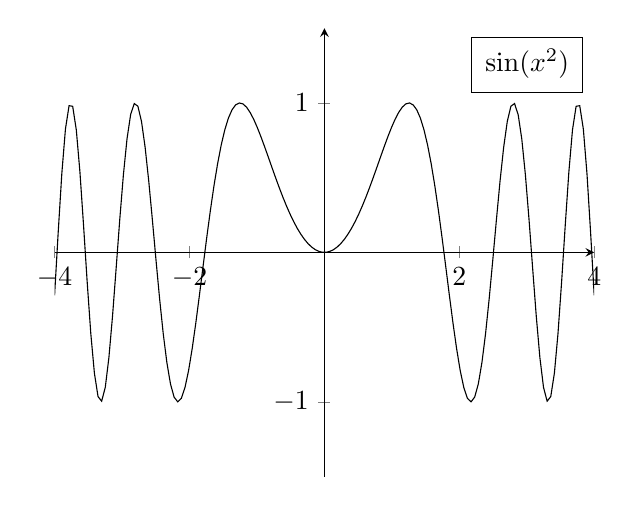
\begin{tikzpicture}
					\begin{axis} [
						axis lines = center,
						axis on top=true,
						legend style={empty legend},
						ymin = -1.5,
						ymax = 1.5
					]
						\addplot[domain=-4:4, samples=150] {sin(deg(x^2))};
						\addlegendentry{\raisebox{.5ex}{$\sin({x^2})$}}
					\end{axis}
				\end{tikzpicture}
			}
			\caption{No unif. cont.}
		\end{subfigure}
		\begin{subfigure}{.24\textwidth}
			\centering
			\resizebox{\linewidth}{!}{
				\begin{tikzpicture}
					\begin{axis} [
						axis lines = center,
						axis on top=true,
						legend style={empty legend},
						ymin = -1.5,
						ymax = 1.5
					]
						\addplot[domain=-4:4, samples=150] {(1/x)*sin(deg(x^2))};
						\addlegendentry{\raisebox{.5ex}{$\frac{1}{x}\sin({x^2})$}}
					\end{axis}
				\end{tikzpicture}
			}
			\caption{Sì unif. cont.}
		\end{subfigure}
	\end{figure}
\end{example}
\begin{exercise}
	\label{ex:cont_unif_cont_comparision}
	Confrontare la \fullref{prop:funz_cont_in_ins} con la \fullref{def:funz_unif_cont}
	\begin{solution}
		In \fullref{prop:funz_cont_in_ins} si definiva la continuità della funzione sull'insieme applicando la \fullref{def:funz_cont} a ogni $x_0 \in A$, cioè ogni punto di $A$. Questo non ha particolari implicazioni sul comportamento della funzione, informa solamente sulla continuità in ogni punto di $A$.\\
		\fullref{def:funz_unif_cont} invece prevede, per definizione, la possibilità di scegliere un qualsiasi $x_0$ quando $\varepsilon$ è già stato scelto. Ciò implica che $\varepsilon$ debba essere valido per ogni $x_0 \in A$, non scelto \textit{a priori}.
	\end{solution}
\end{exercise}
\begin{proposition}
	\label{prop:if_unif_cont_then_conf}
	Siano $(X,d_X)$ e $(Y,d_Y)$ spazi metrici. Sia $f:A \to Y$ con $A \subseteq X$.
	\[f \text{ \textbf{Uniformemente Continua} in } A \quad \implies \quad f \text{ \textbf{Continua} in } A\]
	\begin{proof}
		Deriva da \fullref{ex:cont_unif_cont_comparision} in quanto, se è possibile scegliere un qualsiasi $x_0$ quando $\varepsilon$ è già stato fissato, sicuramente sarà possibile fare questa scelta anche in ordine inverso (la continuità è condizione meno stringente).
	\end{proof}
\end{proposition}
\begin{exercise}
	Siano $(X,d_X)$ e $(Y,d_Y)$ spazi metrici e $k \in Y$. Data $f:\; X \to Y$ definita da $f(x) = k \quad \forall x \in X$.\\
	Dimostrare che $f$ è uniformemente continua.
	% TODO solution
\end{exercise}
\begin{exercise}
	Formulare e dimostrare il teorema sulla uniforme continuità della composizione di funzioni uniformemente continue in spazi metrici.
	% TODO solution
\end{exercise}
\begin{example}
	Sia $f:\; \R \to \R$ data da $f(x) = x^2$. $f$ è continua in $\R$, ma \textit{non} è uniformemente continua in $\R$
\end{example}
\begin{exercise}
	Esibire esempi di funzioni $f:\; \R \to \R$ che siano limitate/illimitate ed uniformemente continue.
\end{exercise}
\begin{example}
	Sia $f:\; \intervalopcl{0}{1} \to \R$ data da $f(x) = \sin(\frac{1}{x})$.\\
	In $\intervalopcl{0}{1}$, $f$ è continua e limitata, ma non è uniformemente continua.
\end{example}

\begin{theorem}[di Cantor]
	\index{Teorema!di Cantor}
	\label{teo:cantor}
	Siano $(X,d_X)$ e $(Y,d_Y)$ spazi metrici e sia $f:K \to Y$ con $K \subseteq X$.
	\begin{equation*}
		\left.
		\begin{array}{l}
		K \text{ \textbf{Compatto}} \\
		f \text{ \textbf{Continua} su } K
		\end{array}
		\right\}
		\quad \implies \quad
		f \text{ \textbf{Uniformemente Continua} su } K
	\end{equation*}
	\begin{proof} Per assurdo, negando la conclusione
		\begin{gather*}
			f \text{ non è uniformemente continua in } K\\
			\implies \exists \varepsilon > 0 \text{ tale che } \forall \delta > 0 \quad \exists x', x'' \in K \text{ con } d(x', x'') < \delta \text{ e } d \bigl( f(x'), f(x'') \bigr) > \varepsilon
			\intertext{Ponendo $\delta = \frac{1}{n+1}$ si passa alla successione convergente a $0$, dunque compatibile con il $\delta$ precedente}
			\implies \exists \varepsilon > 0 \text{ tale che } \forall n \in \N \quad \exists x_n', x_n'' \in K \text{ con } \underbrace{d(x_n', x_n'') < \frac{1}{n+1}}_{\text{(1)}} \text{ e } \underbrace{d \bigl( f(x_n'), f(x_n'') \bigr) > \varepsilon}_{\text{(2)}} \tageq\label{eq:th_cantor}
		\end{gather*}
		Essendo $K$ compatto per ipotesi, per le due successioni $x_n'$ e $x_n''$ esistono due sottosuccessioni $x_{n_k}'$ e $x_{n_k}''$ convergenti a $x_\infty', x_\infty'' \in K$.\\
		Da (1) di \cref{eq:th_cantor} si sa che $\lim\limits_{n \to +\infty} d(x_n', x_n'') = 0$, dunque $x_\infty' = x_\infty''$ per $n \to +\infty$\\
		Da (2) di \cref{eq:th_cantor}, d'altro canto, è esplicitato che $d \bigl( f(x_n'), f(x_n'') \bigr)$ rimane sempre $> \varepsilon$ strettamente positivo, dunque è negata la \fullref{def:funz_cont} in $x_\infty' = x_\infty''$. Così è negata l'ipotesi sulla continuità della funzione.
	\end{proof}
\end{theorem}
\begin{proposition}
	Siano $(X,d_X)$ e $(Y,d_Y)$ spazi metrici, $A \subseteq X$ e $f:A \to Y$ \textbf{Uniformemente Continua} su $A$. Allora, per ogni successione $x:\N \to X$ \textbf{di Cauchy} in $X$, la successione $f \circ x$ delle immagini $f(x_n)$ \textbf{è di Cauchy} in $Y$.
	\begin{proof}
		Omessa.
	\end{proof}
\end{proposition}
\begin{proposition}
	Siano $(X,d_X)$ e $(Y,d_Y)$ spazi metrici, $A \subseteq X$ e $f:A \to Y$ \textbf{Uniformemente Continua} su $A$. Allora esiste un'unica funzione
	\[\overline{f}: \overline{A} \to Y\]
	continua su $\overline{A}$ e tale che $f_{|A} = f$ (cioè la $f$ ristretta ad $A$, dove definita, corrisponde a $f$)
	\begin{proof}
		Omessa.
	\end{proof}
\end{proposition}

\subsection{Lipschitzianità}
\begin{definition}[Funzione Lipschitziana]
	\index{Funzione!Lipschitziana}
	\label{def:lips}
	Siano:
	\begin{itemize}[noitemsep]
		\item $(X,d_X)$, $(Y,d_Y)$ spazi metrici
		\item $A \subseteq X$
		\item $f:A \to Y$
	\end{itemize}
	Allora
	\begin{equation*}
		\begin{gathered}
			f \text{ è \textbf{Lipschitziana}}\\
			\bydef\\
			\exists L > 0:\; \forall x',\,x'' \in X, \quad d_Y\bigl(f(x''),f(x')\bigr) \leq L \cdot d_X(x'',x')
		\end{gathered}
	\end{equation*}
	\begin{note}
		La costante $L$ sopra introdotta non è univocamente determinata. Nei risultati seguenti non sarà mai rilevante \textit{il valore} di $L$, ma il fatto stesso che $L$ esista.
	\end{note}
\end{definition}
\begin{definition}[Costante di Lipschitz]
	\index{Costante di Lipschitz}
	\label{def:cost_lips}
	Fissate le distanze $d_X$ e $d_Y$ e la funzione $f$, allora \textbf{la più piccola} $L$ positiva soddisfacente
	\[d_Y\bigl(f(x''),f(x')\bigr)\leq L \cdot d_X(x'',x') \qquad \forall x',x'' \in X\]
	si definisce \textbf{Costante di Lipschitz} della funzione $f$ in $X$.
\end{definition}
\begin{example}
	\label{ex:lips_graphs}
	~
	\begin{figure}[H]
		\begin{subfigure}{.24\textwidth}
			\centering
			\resizebox{\linewidth}{!}{
				\begin{tikzpicture}
					\begin{axis} [
						axis lines = center,
						axis on top=true,
						legend style={empty legend}
					]
						\addplot [domain=-3:-2.5] {-x-2};
						\addplot [domain=-2.5:-1.5] {x+3};
						\addplot [domain=-1.5:-.5] {-x};
						\addplot [domain=-.5:1] {x+1};
						\addplot [domain=1:1.5] {-x+3};
						\addplot [domain=1.5:3] {x};
					\end{axis}
				\end{tikzpicture}
			}
			\caption{Sì lips.}
		\end{subfigure}
		\begin{subfigure}{.24\textwidth}
			\centering
			\resizebox{\linewidth}{!}{
				\begin{tikzpicture}
					\begin{axis} [
						axis lines = center,
						axis on top=true,
						legend style={empty legend}
					]
						\addplot [domain=-2:2,samples=100] {x^2};
						\addlegendentry{\raisebox{.5ex}{$x^2$}}
					\end{axis}
				\end{tikzpicture}
			}
			\caption{No lips.}
		\end{subfigure}
		\begin{subfigure}{.24\textwidth}
			\centering
			\resizebox{\linewidth}{!}{
				\begin{tikzpicture}
					\begin{axis} [
						axis lines = center,
						axis on top=true,
						ymin = -2,
						ymax = 2
					]
						\addplot[domain=-2:0, samples=10] {1};
						\addplot[domain=0:2, samples=10] {-1};
						\addplot [only marks, mark=*] coordinates{(0,-1)};
						\addplot [fill=white, only marks,mark=*] coordinates{(0,1)};
					\end{axis}
				\end{tikzpicture}
			}
			\caption{No lips.}
		\end{subfigure}
		\begin{subfigure}{.24\textwidth}
			\centering
			\resizebox{\linewidth}{!}{
				\begin{tikzpicture}
					\begin{axis} [
						axis lines = center,
						axis on top=true,
						legend style={empty legend}
					]
						\addplot [domain=0:.2,samples=100,smooth] {sqrt(x)};
						\addplot [domain=.2:3,samples=50] {sqrt(x)};
						\addlegendentry{\raisebox{.5ex}{$\sqrt{x}$}}
					\end{axis}
				\end{tikzpicture}
			}
			\caption{No lips.\\(Sì unif. cont.)}
		\end{subfigure}
	\end{figure}
\end{example}
\begin{example}
	Sono dati gli spazi metrici $(X,d_X)$ e $(Y,d_Y)$ ed una funzione Lipschitziana $f: X \to Y$.\\
	Determinare una nuova distanza $\delta_X$ su $X$ che sia equivalente a $d_X$ ed in modo che la costante di Lipschitz di $f$ rispetto a $\delta_X$ sia minore o uguale ad $1$.
	% TODO solution
\end{example}
\begin{example}
	Sono dati gli spazi metrici $(X,d_X)$ e $(Y,d_Y)$ ed una funzione Lipschitziana $f: X \to Y$.\\
	Determinare una nuova distanza $\delta_Y$ su $Y$ che sia equivalente a $d_Y$ ed in modo che la costante di Lipschitz di $f$ rispetto a $\delta_Y$ sia minore o uguale ad $1$.
	% TODO solution
\end{example}
\begin{exercise}
	Sia $f: \R \to \R$. Come si fa a capire se $f$ è Lipschitziana o no dal suo grafico?
\end{exercise}

\begin{proposition}
	\label{prop:convesso_deriv_par_lim_allora_lips}
	Siano $A \subseteq \R^n$ un insieme \textbf{Convesso} (da \fullref{def:convesso}) e $f \in \cntclass{1}(A;\R)$ (da \fullref{def:cnt_class_1}). Se tutte le \textbf{Derivate Parziali} sono \textbf{limitate} in $A$ , allora $f$ è \textbf{Lipschitziana}.
	\begin{proof}
		Segue direttamente da \fullref{def:convesso} e \fullref{teo:accresc_fin}.
	\end{proof}
\end{proposition}

\begin{proposition}
	\label{prop:se_lips_allora_unif_cont}
	Sia $f: X \to Y$ una funzione \textbf{Lipschitziana}. Allora $f$ è \textbf{Uniformemente Continua} su $X$.
	\begin{proof}
		Dall'ipotesi di Lipschitzianità, applicando la \fullref{def:lips}, si sa per certo che
		\[d_Y\bigl(f(x''),f(x')\bigr) \leq L \cdot d_X(x'',x')\]
		Posti ora
		\begin{itemize}
			\item $d_X(x'',x') < \delta$ senza perdere generalità (il $\delta$ nella unif. continuità è a scelta)
			\item $\delta = \frac{\varepsilon}{L}$ come semplice posizione
		\end{itemize}
		Si ottiene
		\[d_Y\bigl(f(x''),f(x')\bigr) \leq L \cdot d_X(x'',x') < L \cdot \delta = L \cdot \frac{\varepsilon}{L} = \varepsilon\]
		Da cui, prendendo il primo e l'ultimo membro,
		\[d_Y\bigl(f(x''),f(x')\bigr) < \varepsilon\]
		che è la condizione di uniforme continuità.
	\end{proof}
\end{proposition}
\begin{example}
	La funzione
	\[\funcdef{f}{\intervalclop{0}{+\infty}}{\R}{x}{\sqrt{x}}\]
	è uniformemente continua ma non è Lipschitziana. Vedere grafico in \fullref{ex:lips_graphs}
\end{example}
\begin{example}
	La funzione
	\[\funcdef{f}{\R}{\R}{x}{\begin{cases}
		\begin{array}{ll}
			x \cdot \sin \left(\frac{1}{x}\right) & \text{se } x \neq 0\\
			0 & \text{se } x = 0\\
		\end{array}
	\end{cases}}\]
	è uniformemente continua ma non è Lipschitziana.
\end{example}
\begin{example}
	La funzione
	\[\funcdef{f}{\intervalclop{0}{+\infty}}{\R}{x}{x^2}\]
	è di classe $\cntclass{\infty}$ ma non è Lipschitziana. Vedere grafico in \fullref{ex:lips_graphs}
\end{example}
\begin{example}
	La funzione
	\[\funcdef{f}{\intervalclop{0}{+\infty}}{\R}{x}{\abs{x}}\]
	è Lipschitziana ma non è derivabile in $0$.
\end{example}
\begin{exercise}
	\label{ex:comp_funz_lips}
	La composizione di funzioni Lipschitziane è Lipschitziana?\\
	Per funzioni reali di variabile reale, la somma/il prodotto di funzioni Lipschitziane è una funzione Lipschitziana?\\
	Enunciare formalmente e dimostrare.
	% TODO solution
\end{exercise}

\begin{proposition}
	Siano $(X,d_X)$ e $(Y,d_Y)$ spazi metrici. Sia $f:A \to \R^n$ con $A \subseteq X$.
	\begin{equation*}
		f \text{ è \textbf{Lipschitziana}} \quad \iff \quad \text{\textbf{ogni componente di} } f \text{ \textbf{è Lipschitziana}}
	\end{equation*}
	\begin{proof}
		Immediata.
		% TODO actual proof
	\end{proof}
\end{proposition}

\begin{definition}[Norma di Matrice]
	\index{Norma!di Matrice}
	\label{def:norm_matr}
	Sia $A \in \mat (m \times n)$. \textbf{Norma} di $A$ è la quantità
	\[\norm{A} = \;\; \max\limits_{\raisebox{-1ex}{${\scriptstyle x \in \overline{B(0,1)} }$}} \; \norm{A \; x}\]
	con $x$ vettore $\in \R^n$ e $A \; x \in \R^m$ risultato del prodotto righe per colonne.
\end{definition}
\begin{exercise}
	Verificare che la norma introdotta in \fullref{def:norm_matr} soddisfi alle condizioni della \fullref{def:norma} con $V = \mat (m \times n)$
\end{exercise}
\begin{exercise}
	\label{ex:matr_form_alt}
	Con la notazione della \fullref{def:norm_matr}, verificare le seguenti uguaglianze
	{
	\renewcommand*{\arraystretch}{1.5} % To improve the spacing of this array
	\begin{equation*}
		\begin{array}{rll}
			\norm{A}	& =\sup\limits_{\raisebox{-1ex}{${\scriptstyle x \in \overline{B(0,1)} }$}} \; \norm{A \; x}	& =\sup\limits_{x \in B(0,1)} \; \norm{A \; x}\\
						& =\max\limits_{\norm{x} = 1} \; \norm{A \; x}													& =\sup\limits_{\norm{x} = 1} \; \norm{A \; x}\\
						& =\sup\limits_{x \in \R^n \setminus \brackets{0}} \frac{\norm{A \; x}}{\norm{x}}
		\end{array}
	\end{equation*}
	}
	% TODO solution
\end{exercise}

\begin{proposition}
	\label{prop:proprieta_norm_matr}
	Sia $A \in \mat(m \times n)$. Allora
	\[\norm{A \; x} \leq \norm{A} \cdot \norm{x}\]
	\begin{proof}
		Sia $x = 0$ la tesi è immediata.\\
		Sia $x \neq 0$, allora
		\begin{align*}
			\norm{A \; x} &= \norm{A \; x \cdot \frac{\norm{x}}{\norm{x}}} = \norm{\norm{x} \cdot \left( A \frac{x}{\norm{x}} \right)}\\
			&= \norm{x} \cdot \norm{A \frac{x}{\norm{x}}}
			\intertext{Essendo $\frac{x}{\norm{x}}$ il versore di $x$, esso ha, per definizione, norma unitaria e, grazie a \fullref{ex:matr_form_alt}, si sa che $\norm{A} \leq \sup\limits_{\norm{x} = 1} \; \norm{A \; x}$, dunque}
			&\leq \norm{A} \cdot \norm{x}
		\end{align*}
	\end{proof}
\end{proposition}
\begin{exercise}
	Esibire una matrice $A \in \mat(2 \times 3)$ tale che $\norm{A} = 2$
	% TODO solution
\end{exercise}
\begin{exercise}
	\label{ex:se_f_in_R_lin_then_lips}
	Sia $f:\R^n \to \R^n$ una funzione \textbf{Lineare}. Allora è \textbf{Lipschitziana} (rispetto alla Metrica Euclidea). Suggerimento: utilizzare la \fullref{prop:proprieta_norm_matr}
	\begin{note}
		In spazi più generali di $\R^n$ (spazi di dimensione \textit{infinita}) l'affermazione contenuta in questo esercizio può essere falsa. Vedasi \fullref{prop:operat_D_non_cont}
	\end{note}
	% TODO solution
\end{exercise}
\begin{exercise}[Disuguaglianza di Cauchy-Schwarz]
	\label{ex:disug_cau_schwa_matr}
	\index{Disuguaglianza!Cauchy-Schwarz}
	Se $A$ e $B$ sono matrici tali che se ne possa fare il prodotto (regole del prodotto righe per colonne), dimostrare che
	\[\norm{A \cdot B} \leq \norm{A} \cdot \norm{B}\]
	\vspace*{-1.5\baselineskip}
	\begin{note}
		Questa è una forma specifica per le matrici della Disuguaglianza di Cauchy-Schwarz, che è più generale ed applicabile anche ad altri enti.
	\end{note}
	% TODO solution
\end{exercise}

\newpage
\section{Il Teorema delle Contrazioni}
\begin{definition}[Contrazione]
	\index{Contrazione}
	\label{def:contrazione}
	Sia $(X, d)$ uno spazio metrico. Si dice \textbf{Contrazione} una funzione $T:\; X \to X$ soddisfacente a:
	\begin{equation}
		\label{eq:def_contrazione}
		\exists K \in [0, 1[ \;: \quad \forall x',x'' \in X \quad \text{vale} \quad d_X \bigl( T(x''), T(x') \bigr) \leq K \cdot d_X(x'', x')
	\end{equation}
	Una contrazione è quindi una funzione con insieme di partenza e di arrivo coincidenti e Lipschitziana con costante di Lipschitz strettamente minore di $1$.\\
	È generalmente inutile considerare contrazioni definite tra spazi diversi. Infatti, data una funzione $T: X \to Y$ Lipschitziana, sarebbe sempre possibile riscalare la distanza in uno dei due spazi $X$ o $Y$ per ottenere una costante di Lipschitz minore di $1$.
	\begin{note}
		D'ora in poi si utilizzerà spesso la notazione $Tx$ per intendere $T(x)$
	\end{note}
\end{definition}
\begin{example}[Esempi di Contrazioni]\leavevmode\vspace*{-\baselineskip}
	\begin{enumerate}
		\item $f: \R \to \R$ data da $f(x) = \frac{x}{2}$. $f$ è una contrazione.
		\item $f: \intervalclose{0}{2} \to \intervalclose{0}{2}$ data da $f(x) = 1 + \frac{x}{2}$. $f$ è una contrazione
		\item $f: \R^2 \to \R^2$ data da $f(x,y)=
			\begin{bmatrix}
				\frac{1}{3} & 0\\[1ex]
				0 & \frac{1}{5}
			\end{bmatrix} \cdot
			\begin{bmatrix}
				x\\[1ex]
				y
			\end{bmatrix}$. $f$ è una contrazione
	\end{enumerate}
\end{example}
\begin{exercise}
	La composizione di contrazioni è una contrazione. Enunciare formalmente e dimostrare.\\
	Esibire esempi che mostrino come la somma ed il prodotto di contrazioni possano non essere contrazioni.
	\begin{solution}\hfill\\
		Sia $(X, d)$ uno spazio metrico, siano $f,g:X \to X$ \textbf{due contrazioni} in $X$. Allora $f\circ g$ è una \textbf{contrazione}
		\begin{proof}
			\renewcommand\qedsymbol{$\square$}
			Sappiamo che:
			\begin{equation*}
				\begin{gathered}
					\forall x',x'' \in X,\; d \bigl( f(x''), f(x') \bigr) \leq K_f \cdot d(x'', x')\\
					\forall x',x'' \in X,\; d \bigl( g(x''), g(x') \bigr) \leq K_g \cdot d(x'', x').
				\end{gathered}
			\end{equation*}
			$f \circ g=f\bigl( g(x) \bigr)$, quindi presi $x',x''\in X$ si ha
			\[d \Bigl( f\bigl(g(x'')\bigr), f\bigl(g(x')\bigr) \Bigr) \leq K_f \cdot d \bigl( g(x''), g(x') \bigr) \leq K_f K_g \cdot d(x'',x')\]
		\end{proof}
		\noindent Esempi: % TODO esempi
	\end{solution}
\end{exercise}

\begin{proposition}
	\label{prop:se_Df_leq_k_allora_f_contr}
	Sia $f \in \cntclass{1}(\R^n;\R^n)$ (da \fullref{def:cnt_class_1}). Se esiste $k \in \intervalclop{0}{1}$ tale che per ogni $x \in \R^n$ vale $\norm{Df(x)} < k$, allora $f$ è \textbf{Contrazione}.
	\begin{proof}
		Segue dal \fullref{teo:accresc_fin}
	\end{proof}
\end{proposition}

\begin{definition}[Punto Fisso]
	\index{Punto!Fisso}
	\label{def:punto_fisso}
	Sia $X$ un insieme e $f: X \to X$. Un \textbf{Punto Fisso} di $f$ è un elemento $x \in X$ tale che:
	\[x=f(x)\]
\end{definition}

\begin{theorem}[delle Contrazioni]\leavevmode\vspace*{-\baselineskip}
	\index{Teorema!delle Contrazioni}
	\index{Teorema!di Banach-Caccioppoli}
	\label{teo:contrazioni}
	\begin{note}
		Questo teorema è anche noto come \textit{Teorema di Banach-Caccioppoli}
	\end{note}
	Sia $(X, d)$ uno spazio metrico e $T: X \to X$. Allora
	\begin{equation*}
		\left.
			\begin{array}{l}
				X \text{ \textbf{Completo}}\\
				T \text{ \textbf{Contrazione}}
			\end{array}
		\right\}
		\quad \implies \quad
		\exists! \; x_* \in X: \quad T(x_*) = x_*
	\end{equation*}
	Cioè esiste un \textbf{unico Punto Fisso} di $T$ in $X$.
	\begin{proof}
		La dimostrazione si divide in 3 passaggi
		\begin{enumerate}
			\item \textit{Individuazione di una Successione di Cauchy}\\
				Dato un generico $x_0 \in X$ si costruisce una successione $x$ nel seguente modo:
				\begin{equation}
					\label{eq:teo_contraz_succ}
					\begin{matrix}x_0 \in X & \quad & x_1 = T(x_0) & \quad & x_2 = T(x_1) & \quad & \dotsc & \quad & x_{n+1} = T(x_n)\end{matrix}
				\end{equation}
				La  successione $x:\N \to X$ è sicuramente ad elementi in $X$ in quanto $T$, contrazione, è per definizione $T: X \to X$. È necessario dimostrare che la $x$ sia di Cauchy (\fullref{def:succ_cau}) cioè che:
				\[\forall \varepsilon > 0\quad \exists \nu \in \N:\; \forall n,m > \nu \text{ vale } d(x_n, x_m) < \varepsilon\]
				Presi ora due qualunque $n$ e $m$ e sfruttando il modo in cui è definita la successione $x$:
				\begin{align*}
					d(x_n, x_m) &= d \bigl( T(x_{n-1}), T(x_{m-1}) \bigr)
					\shortintertext{Grazie al fatto che $T$ è contrazione, per definizione esiste un $K \in \intervalclop{0}{1}$ per cui}
					&\leq K \cdot d(x_{n-1}, x_{m-1})
					\shortintertext{Ripetendo gli ultimi due passaggi, si continua}
					&= d \bigl( T(x_{n-2}), T(x_{m-2}) \bigr)\\
					&\leq K^2 \cdot d(x_{n-2}, x_{m-2})
					\shortintertext{Ipotizzando ora $n < m$, sicuramente dopo un $n$ numero di passi analoghi si arriverà a $0$}
					&\leq K^n \cdot d(x_0, x_{m-n})
				\end{align*}
				Quindi, andando dal primo all'ultimo passaggio, si è ottenuta la disuguaglianza
				\begin{equation}
					\label{eq:teo_contraz_disug_dist_mn}
					d(x_n, x_m) \leq K^n \cdot d(x_0, x_{m-n})
				\end{equation}
				Ora, applicando ripetutamente la disuguaglianza triangolare al secondo membro della \cref{eq:teo_contraz_disug_dist_mn}
				\begin{align*}
					K^n \cdot d(x_0, x_{m-n}) &\leq K^n \cdot \Bigl( d(x_0, x_1) + d(x_1, x_2) + \dotsc + d(x_{m-n-1}, x_{m-n}) \Bigr)
					\shortintertext{Applicando ora quanto ottenuto in \cref{eq:teo_contraz_disug_dist_mn} a tutti gli addendi}
					&\leq K^n \cdot \Bigl( K^0 \cdot d(x_0, x_1) + K^1 \cdot d(x_0, x_1) + \dotsc + K^{m-n-1} \cdot d(x_0, x_1) \Bigr)\\
					&= K^n \cdot \Bigl( 1 + K + \dotsc + K^{m-n-1} \Bigr) \cdot d(x_0, x_1)
				\end{align*}
				Quindi riassumendo, partendo dal primo membro dalla \cref{eq:teo_contraz_disug_dist_mn}, si è arrivati a
				\begin{equation}
					\label{eq:teo_contraz_disug_dist_mn_fin}
					d(x_n, x_m) \leq K^n \cdot \Bigl( \underbrace{1 + K + \dotsc + K^{m-n-1}}_{\text{(1)}} \Bigr) \cdot d(x_0, x_1)
				\end{equation}

				Posta ora la (1) di \cref{eq:teo_contraz_disug_dist_mn_fin} come $s$ si ha:
				\[s = 1 + K + \dotsc + K^{m-n-1} \qquad \text{e, moltiplicando per } K \text{,} \qquad K \cdot s = K + K^2 + \dotsc + K^{m-n}\]
				Da cui, eseguendo la differenza tra $s$ e $K \cdot s$
				\begin{align*}
					&s - K \cdot s\\
					= &\Bigl( 1 + \cancel{K} + \cancel{\dotsc} + \cancel{K^{m-n-1}} \Bigr) - \Bigl( \cancel{K} + \cancel{K^2} + \cancel{\dotsc} + K^{m-n} \Bigr)\\
					= &1 - K^{m-n}
				\end{align*}
				si ottiene l'equivalenza
				\begin{align*}
					s - K \cdot s &= 1 - K^{m-n}\\
					s (1 - K) &= 1 - K^{m-n}\\
					s &= \frac{1 - K^{m-n}}{1 - K}
				\end{align*}
				Sostituendo la formulazione di $s$ appena trovata in \cref{eq:teo_contraz_disug_dist_mn_fin} si ottiene
				\begin{equation}
					\label{eq:teo_contraz_disug_s}
					d(x_n, x_m) \leq K^n \cdot \frac{1 - K^{m-n}}{1 - K} \cdot d(x_0, x_1)
				\end{equation}
				Essendo $K \in \intervalclop{0}{1}$, eseguendone l'elevamento a potenza otterrò un numero ancor più piccolo. È dunque certo che
				\[1 - K^{m-n} \geq 1 - K \implies \frac{1 - K^{m-n}}{1 - K} \leq 1\]
				per cui è sicuramente possibile minorare la \cref{eq:teo_contraz_disug_s} che diventa
				\begin{equation}
					\label{eq:teo_contraz_disug_dist_01}
					d(x_n, x_m) \leq K^n \cdot d(x_0, x_1)
				\end{equation}
				\vspace*{-4ex}
				\begin{note}
					\hypertarget{note:teo_contraz_note}{}
					La \cref{eq:teo_contraz_disug_dist_01}, per come è scritta, fornisce un importante risultato. Grazie a questa equazione, noto $n$ e calcolando solo la distanza tra gli elementi $0$ ed $1$ della successione (facilmente individuabili) si ha un limite superiore per la $d(x_n, x_m) \; \forall n,m$. Non sarebbe stato invece possibile calcolare la $d(x_0, x_{n-m})$ trovata ancora prima.
				\end{note}
				Questa minorazione permette di verificare la definizione di successione di Cauchy, dunque la $x$ definita in \cref{eq:teo_contraz_succ} è di Cauchy.
				\qed
			\item \textit{Individuazione del Punto Fisso}\\
				La successione $x$ definita in \cref{eq:teo_contraz_succ}, essendo stata dimostrata di Cauchy nel passo precedente, per \fullref{def:completo} ammette sicuramente $\lim\limits_{n \to +\infty} x_n = x_* \in X$. Inoltre
				\[
					T \text{ Contrazione}
					\quad \overset{
						\mathclap{
							\rule[-\baselineskip]{0pt}{\baselineskip}
							\text{
								\begin{tabular}{c}
									Come da\\[-1ex]
									\fullref{def:contrazione}
								\end{tabular}
							}
						}
					}{\implies} \quad T \text{ Lipschitziana}
					\quad \overset{
						\mathclap{
							\rule[-\baselineskip]{0pt}{\baselineskip}
							\text{
								\begin{tabular}{c}
									Per\\[-1ex]
									\fullref{prop:se_lips_allora_unif_cont}
								\end{tabular}
							}
						}
					}{\implies} \quad T \text{ Unif. Cont.}
					\quad \overset{
						\mathclap{
							\rule[-\baselineskip]{0pt}{\baselineskip}
							\text{
								\begin{tabular}{c}
									Per\\[-1ex]
									\fullref{prop:if_unif_cont_then_conf}
								\end{tabular}
							}
						}
					}{\implies} \quad T \text{ Continua}
				\]
				Posto quindi
				\begin{align*}
					T(x_*) &= T \bigl( \; \lim\limits_{n \to +\infty} x_n \; \bigr)
					\shortintertext{Grazie alla continuità di $T$}
					&= \lim\limits_{n \to +\infty} \bigl(T(x_n)\bigr)
					\shortintertext{Dunque, per come è definita $x$}
					&= \lim\limits_{n \to +\infty} ( x_{n+1} )\\
					&= x_*
				\end{align*}
				\qed
			\item \textit{Dimostrazione unicità punto fisso}\\
				Si suppone non sia unico
				\[x_0, y_0 \in X \;\; x_0 \neq y_0 \qquad T(x_0) = x_0,\; T(y_0) = y_0\]
				Calcolando la distanza tra i due punti, sfruttando il fatto che siano punti fissi per definizione ed, infine, essendo $T$ contrazione si ottiene
				\begin{equation*}
					\begin{gathered}
						d(x_0, y_0) = d\bigl( T(x_0), T(y_0) \bigr) \leq K \cdot d(x_0, y_0)\\
						d(x_0, y_0) - K \cdot d(x_0, y_0) \leq 0
					\end{gathered}
				\end{equation*}
				\begin{equation}
					\label{eq:teo_contraz_unicita}
					(1-K) \bigl( d(x_0, y_0) \bigr) \leq 0
				\end{equation}
				Però
				\begin{itemize}
					\item $1-K > 0$ strettamente positivo perché, per \fullref{def:contrazione} $K \in \intervalclop{0}{1}$
					\item $d(x_0, y_0) \geq 0$ per \fullref{def:sp_metrico}
				\end{itemize}
				Allora deve essere per forza $d(x_0, y_0) = 0$ per non contraddire la \cref{eq:teo_contraz_unicita}, dunque, per proprietà \ref{itm:dist_0_iff_x_uguale_y} delle distanze (\fullref{def:sp_metrico}), $x_0 = y_0$.
				% No need for QED symbol here since one is provided by the proof environment
		\end{enumerate}
	\end{proof}
\end{theorem}
\begin{exercise}
	I passaggi da \cref{eq:teo_contraz_disug_dist_mn} a \cref{eq:teo_contraz_disug_dist_01} sono necessari?
	\begin{solution}
		Vedere \hyperlink{note:teo_contraz_note}{\notestyle{} alla dimostrazione del \fullref*{teo:contrazioni}}
	\end{solution}
\end{exercise}
\begin{example}
	Se $X$ \textit{non} è completo:\\
	Siano $X = \intervalopen{0}{1}$ e $T: X \to X$ data $T(x) = \frac{x}{2}$. $T$ è una contrazione senza punti fissi in $X$
\end{example}
\begin{example}
	Se $T$ è \textit{quasi} una contrazione possono non esserci punti fissi:\\
	Sia $X = \R$ e sia $T:X \to X$ data da $T(x) = x + \frac{\pi}{2} - \arctan x$. Grazie \fullref{teo:lagrange} (da Analisi 1, essendo in $\R$) si può facilmente dimostrare che $\forall x', x'' \in X$
	\[\abs{T(x'') - T(x')} < \abs{x'' - x'}\]
	però $T$ non è una contrazione ed infatti non ammette punti fissi.
\end{example}
\begin{example}
	Se $T$ è \textit{quasi} una contrazione possono esserci infiniti punti fissi:\\
	Sia $X = \R$ e sia $T:X \to X$ data da $T(x) = x$. Evidentemente
	\[\abs{T(x'') - T(x')} = \abs{x'' - x'}\]
	e $T$ ammette infiniti punti fissi.
\end{example}
\begin{exercise}
	Sia $f \intervalclose{0}{1} \to \intervalclose{1}{2}$ data da $f(x) = 1 + \frac{x}{2}$\\
	$f$ è una funzione Lipschitziana con costante di Lipschitz $\frac{1}{2}$ definita tra spazi metrici completi ma senza punti fissi. È in contraddizione con il \fullref{teo:contrazioni}?
	% TODO solution
\end{exercise}
\begin{exercise}
	Sia $f:\R \to \R$ derivabile su $\R$ e tale che $f'(x) \leq \frac{1}{2} \quad \forall x \in \R$.\\
	Dimostrare che allora esiste un unico $x_* \in \R$ tale che $f(x_*) = x_*$
	\begin{solution}
		$\R$ è Completo come da \fullref{ex:sp_metr_compl_e_non}, inoltre la $f$ è Contrazione per \fullref{prop:se_Df_leq_k_allora_f_contr}, dunque è possibile applicare il \fullref{teo:contrazioni} ed arrivare alla tesi.
	\end{solution}
\end{exercise}

\begin{observation}
	\label{obs:contr_con_para}
	È utile considerare \textbf{contrazioni} che dipendono da uno o più \textbf{parametri}. Siano $(X,d)$ uno spazio metrico completo, $P$ un \textbf{insieme} di parametri e $T:X \times P \to X$.\\
	Grazie al \fullref{teo:contrazioni} è data l'esistenza di un punto fisso di $T$ indipendentemente dal parametro. È dunque possibile definire una funzione $\varphi: P \to X$ che ad ogni parametro $p \in P$ associa $\varphi(p)$, unico punto fisso della contrazione.\\
	In generale, la regolarità della funzione $\varphi$ è la stessa con cui $T$ dipende dal parametro $p$. Vedasi \fullref{teo:contrazioni_con_para} e \fullref{teo:contr_con_para_lips_definisce_funz_lips}
\end{observation}

\begin{definition}[Contrazione con Parametro]
	\index{Contrazione!con Parametro}
	\label{def:contrazione_parametro}
	Siano $(X,d)$ uno \textbf{Spazio Metrico} e $P$ un \textbf{Insieme}
	\begin{equation}
		\label{eq:contrazione_parametro}
		\begin{gathered}
			T \text{ è una \textbf{Contrazione} in } x \in X \text{ \textbf{Uniformemente} in } p \in P\\
			\bydef\\
			\exists K \in \intervalclop{0}{1}: \; \forall p \in P,\; \forall x', x'' \in X \quad \text{vale} \quad d \Bigl( T\bigl( x', p \bigr), T\bigl( x'', p \bigr) \Bigr) \leq K \cdot d(x', x'')
		\end{gathered}
	\end{equation}
	Cioè, indipendentemente da qualsiasi $p \in P$, la $T$ rimane contrazione.
\end{definition}

\cbstart
\begin{theorem}[delle Contrazioni con Parametro]
	\index{Teorema!delle Contrazioni con Parametro}
	\label{teo:contrazioni_con_para}
	Siano:
	\begin{itemize}[noitemsep]
		\item $(X,d_X)$ uno spazio metrico completo
		\item $(P,d_P)$ uno spazio metrico
		\item $T:X \times P \to X$ una contrazione in $x \in X$ uniformemente in $p \in P$
		\item $T$ continua
	\end{itemize}
	Allora $\forall p \in P$ esiste un unico punto fisso $x_p$ per la funzione $x \mapsto T(x,p)$ e la funzione $P \to X_p$ è continua.
	\begin{proof}
		Come già detto in \fullref{obs:contr_con_para}, il \fullref{teo:contrazioni} assicura l'esistenza di una funzione $\varphi: P \to X$ che ad ogni $p \in P$ associa un unico punto fisso di $x \mapsto T(x,p)$. $\varphi$ è continua. Infatti se $p_n \to p_0$
		\begin{align*}
					&d_X \bigl( \varphi(p_n), \varphi(p_0) \bigr) =
			\shortintertext{Essendo $\varphi(p_n)$ per definizione punto fisso di $T$ con parametro $p_n$}
			=\;\;	&d_X \Bigl( T \bigl( \varphi(p_n), p_n \bigr), T \bigl( \varphi(p_0), p_0 \bigr) \Bigr)
			\shortintertext{Applicando la disuguaglianza triangolare}
			\leq\;\;&d_X \Bigl( T \bigl( \varphi(p_n), p_n \bigr), T \bigl( \varphi(p_0), p_n \bigr) \Bigr) +
					d_X \Bigl( T \bigl( \varphi(p_0), p_n \bigr), T \bigl( \varphi(p_0), p_0 \bigr) \Bigr)
			\shortintertext{Con la definizione di contrazioni}
			\leq\;\;&K \cdot d_X \bigl( \varphi(p_n), \varphi(p_0) \bigr) +
					d_X \Bigl( T \bigl( \varphi(p_0), p_n \bigr), T \bigl( \varphi(p_0), p_0 \bigr) \Bigr)
		\end{align*}
		Dunque
		\[d_X \bigl( \varphi(p_n), \varphi(p_0) \bigr) \leq K \cdot d_X \bigl( \varphi(p_n), \varphi(p_0) \bigr) + d_X \Bigl( T \bigl( \varphi(p_0), p_n \bigr), T \bigl( \varphi(p_0), p_0 \bigr) \Bigr)\]
		Da cui, infine
		\[d_X \bigl( \varphi(p_n), \varphi(p_0) \bigr) \leq \frac{1}{1-K} \cdot d_X \Bigl( T \bigl( \varphi(p_0), p_n \bigr), T \bigl( \varphi(p_0), p_0 \bigr) \Bigr)\]
		Ed il secondo membro tende a $0$ per $n \to +\infty$ grazie alla continuità di $T$, quindi da \fullref{prop:cont_e_cont_per_succ} la $\varphi$ è continua.
	\end{proof}
\end{theorem}

\begin{definition}[Contrazione Lipschitziana in Parametro]
	\index{Contrazione!Lipschitziana in Parametro}
	\label{def:contr_lips_para}
	Siano $(X,d_X)$ e $(P,d_P)$ spazi metrici
	\begin{equation*}
		\begin{gathered}
			T \text{ è una \textbf{Contrazione} in } x \in X \text{ \textbf{Lipschitziana} in } p \in P\\
			\bydef\\
			\exists K \in \intervalclop{0}{1}, \exists L > 0: \; \forall p', p'' \in P, \forall x', x'' \in X \text{ vale}\\
			d_X \bigl( T( x', p'), T(x'', p'') \bigr) \leq K \cdot d_X(x', x'') + L \cdot d_P (p', p'')
		\end{gathered}
	\end{equation*}
	Cioè, si aggiunge la Lipschitzianità rispetto al parametro
\end{definition}
\begin{theorem}
	\label{teo:contr_con_para_lips_definisce_funz_lips}
	Siano:
	\begin{itemize}[noitemsep]
		\item $(X,d_X)$ uno spazio metrico completo
		\item $(P,d_P)$ uno spazio metrico
		\item $T:X \times P \to X$ una contrazione in $x \in X$ Lipschitziana in $p \in P$
	\end{itemize}
	Allora esiste un'unica funzione Lipschitziana $\varphi: P \to X$ tale che $\varphi(p)$ è l'unico punto fisso della funzione $x \mapsto T(x,p)$
	\begin{note}
		L'unicità del punto fisso implica automaticamente l'unicità della funzione $\varphi$
	\end{note}
	\begin{proof}
		Come già detto in \fullref{obs:contr_con_para}, il \fullref{teo:contrazioni} assicura l'esistenza di una funzione $\varphi: P \to X$ che ad ogni $p \in P$ associa un unico punto fisso di $x \mapsto T(x,p)$. $\varphi$ è Lipschitziana. Infatti
		\begin{align*}
			&d_X \bigl( \varphi(p'), \varphi(p'') \bigr) =
			\shortintertext{Essendo $\varphi(p)$ per definizione punto fisso di $T$ con parametro $p$}
			=\;\;	&d_X \Bigl( T \bigl( \varphi(p'), p' \bigr), T \bigl( \varphi(p''), p'' \bigr) \Bigr)
			\shortintertext{Applicando la \fullref{def:contr_lips_para}}
			\leq\;\;&K \cdot d_X \bigl( \varphi(p'), \varphi(p'') \bigr) + L \cdot d_P(p', p'')
		\end{align*}
		Dunque
		\[d_X \bigl( \varphi(p'), \varphi(p'') \bigr) \leq K \cdot d_X \bigl( \varphi(p'), \varphi(p'') \bigr) + L \cdot d_P(p', p'')\]
		Da cui, infine
		\[d_X \bigl( \varphi(p'), \varphi(p'') \bigr) \leq \frac{L}{1-K} \cdot d_P (p', p'')\]
		Che dimostra la Lipschitzianità di $\varphi$
	\end{proof}
\end{theorem}

\begin{exercise}
	Nel presente capitolo, ambientato in spazi metrici, non viene trattata la derivabilità del punto fisso rispetto al parametro. Perché?
	% TODO solution
\end{exercise}

\begin{definition}[Funzione Iterata]
	\index{Funzione!Iterata}
	\label{def:iterata}
	Data $F:X \to X$, si dice \textbf{Funzione Iterata} $n$ volte di $F$ la $F^n$ che corrisponde all'\textbf{applicazione} $n$ volte di $F$ \textbf{su sè stessa}. Formalmente:
	\[f^{n+1} = f \circ f^n \quad \forall n \in \N\setminus\brackets{0}\]
	Se $n = 0$, per definizione, $f^0 = \mathrm{Id}_X$ con $\mathrm{Id}_X$ funzione identità su $X$
\end{definition}

\begin{theorem}[dell'Iterata Contrazione]
	\index{Teorema!dell'Iterata Contrazione}
	\label{teo:iterata_contraz}
	Sia $(X,d_X)$ uno spazio metrico completo e sia $T:X \to X : \exists n \in \N, T^n$ \textbf{Iterata} è contrazione.\\
	Allora $T$ ammette un unico punto fisso in $X$
	\begin{note}
		La $n$ non è univocamente definita e non potrebbe esserlo.\\
		Se infatti $T^n$ è contrazione, allora anche $T^{2n},\, T^{3n},\, \cdots,\, T^{\alpha n}$ lo sono.
	\end{note}
	\begin{proof}
		Per il \fullref{teo:contrazioni} esiste un unico punto fisso $x_* \in X$ per $T^n$, quindi
		\[T^nx_* = x_*\]
		applicando $T$ ad entrambi i membri
		\[T(T^{n}x_*) = Tx_*\]
		e per la \fullref{def:iterata}
		\[T(T^{n}x_*) = T^n(Tx_*) = Tx_*\]
		Dunque $Tx_*$ è punto fisso della $T^n$. Avevamo però già trovato che $x_*$ era punto fisso della $T^n$ e, per il \fullref{teo:contrazioni}, può esistere un unico punto fisso. Ciò permette di concludere che $Tx_* = x_*$
	\end{proof}
\end{theorem}
\begin{exercise}
	Enunciare e dimostrare formalmente il \textit{Teorema dell'Iterata Contrazione con Parametro}
\end{exercise}
\cbend

\newpage
\markright{FUNZIONI A VALORI IN $\R^n$} % To mark current page, in case it's a right page
\section{Funzioni a Valori in \texorpdfstring{$\protect \R^n$}{R\textasciicircum n}}
\markright{FUNZIONI A VALORI IN $\R^n$} % To mark all the following pages, overriding \section's default mark
% \markright is used to change section headings to force the "n" in R^n to lowercase.
% The same couldn't be performed simply by using \MakeLowercase in section's name since it was broken in TOC.

In tutto questo paragrafo si hanno $n \in \N$ e $n \geq 1$. Con $\R^n$ viene indicato lo spazio metrico $\R$ dotato dell'usuale \textbf{Metrica Euclidea}: $d(x,y) = \sqrt{\sum\limits_{i = 1}^{k} (y_i - x_i)^2}$ da \fullref{ex:metriche}.\\
Questo spazio si dice anche \fullref{def:sp_vett_normato}.
\begin{note}
	Diverse dimostrazioni di questo capitolo sono omesse in quanto estremamente simili a quelle di Analisi 1.
\end{note}

\subsection{Il Caso Generale}
\begin{proposition}
	\label{prop:lim_in_R_somma_prod}
	Siano $(X,d)$ uno spazio metrico, $A \subseteq X$, $f:A \to \R^n$, $g:A \to \R^n$ e $x_0$ \textbf{di accumulazione} per $A$, allora se:
	\begin{equation*}
		\left.
		\begin{array}{r}
			\lim\limits_{x \to x_0} f(x) \text{ esiste finito}\\
			\lim\limits_{x \to x_0} g(x) \text{ esiste finito}
		\end{array}
		\right\}
		\implies
		\begin{cases}
			\begin{array}{c}
				\lim\limits_{x \to x_0} (f + g)(x) \quad \exists \text{ finito}\\[-1ex]
				e\\[-1ex]
				\lim\limits_{x \to x_0} (f + g)(x) = \lim\limits_{x \to x_0} f(x) + \lim\limits_{x \to x_0} g(x)\\
				\\
				\lim\limits_{x \to x_0} (f \cdot g)(x) \quad \exists \text{ finito}\\[-1ex]
				e\\
				\lim\limits_{x \to x_0} (f \cdot g)(x) = \lim\limits_{x \to x_0} f(x) \cdot \lim\limits_{x \to x_0} g(x)
			\end{array}
		\end{cases}
	\end{equation*}
	\begin{note}
		$f \cdot g$ indica il prodotto scalare $f \cdot g = \sum\limits_{i = 1}^{n} f_i \cdot g_i$
	\end{note}
	\begin{proof}
		Omessa.
	\end{proof}
\end{proposition}
\begin{exercise}
	Dimostrare la \fullref{prop:lim_in_R_somma_prod}
	\begin{solution}
		Dalla \fullref{def:lim_funz}
		\begin{equation*}
			\begin{gathered}
				\forall \varepsilon > 0,\; \exists \delta_f > 0:\; \forall x \in A \text{ con } d_X(x,x_0) < \delta_f \text{ e } x \neq x_0 \text{ vale } \norm{f(x) - l_f} < \varepsilon\\
				\forall \varepsilon > 0,\; \exists \delta_g > 0:\; \forall x \in A \text{ con } d_X(x,x_0) < \delta_g \text{ e } x \neq x_0 \text{ vale } \norm{g(x) - l_g} < \varepsilon
			\end{gathered}
		\end{equation*}
		Fissato $\varepsilon$, si può scegliere $\delta = \min \brackets{\delta_f, \delta_g}$ e quindi è possibile dire che
		\begin{equation}
			\label{eq:lim_somma_fun}
			\forall \varepsilon > 0,\; \exists \delta: \forall x \in A \text{ con } d_X(x,x_0) < \delta \text{ e } x \neq x_0 \text{ vale } \norm{(f + g)(x) - (l_f + l_g)} < \varepsilon
		\end{equation}
		Essendo
		\begin{align*}
			\norm{(f + g)(x) - (l_f + l_g)} &= \norm{\bigl( f(x) - l_f \bigr) + \bigl( g(x) - l_g \bigr)}
			\shortintertext{Per proprietà \ref{itm:def_norm_propr_somma} da \fullref{def:norma}}
			&\leq \norm{f(x) - l_f} + \norm{g(x) - l_g}
		\end{align*}
		Quest'ultima forma è sicuramente $< \varepsilon$ per \cref{eq:lim_somma_fun}, quindi la somma dei limiti corrisponde al limite della somma.\\
		Analogamente si svolge per il prodotto.
	\end{solution}
\end{exercise}
\begin{exercise}
	Enunciare e dimostrare un analogo della \fullref{prop:lim_in_R_somma_prod} per il prodotto vettoriale
	% TODO solution
\end{exercise}

\begin{proposition}
	\label{prop:lim_in_R_coord_F}
	Siano:
	\begin{itemize}[noitemsep]
		\item $(X,d)$ \textbf{Spazio Metrico}
		\item $A \subseteq X$
		\item $x_0$ \textbf{di Accumulazione} per $A$
		\item $f: A \to \R^n$ e $g: A \to \R^m$
	\end{itemize}
	Posta dunque
	\[\funcdef{F}{A}{\R^{n + m}}{x}{\bigl( f(x),\; g(x) \bigr)}\]
	Allora
	\[
		\left.
		\begin{array}{r}
			\lim\limits_{x \to x_0} f(x) \text{ esiste finito}\\
			\lim\limits_{x \to x_0} g(x) \text{ esiste finito}
		\end{array}
		\right\}
		\implies
		\begin{cases}
			\begin{array}{c}
				\lim\limits_{x \to x_0} F(x) \quad \text{esiste finito}\\
				e\\
				\lim\limits_{x \to x_0} F(x) = \left( \lim\limits_{x \to x_0} f(x), \lim\limits_{x \to x_0} g(x) \right)
			\end{array}
		\end{cases}
	\]
	\begin{proof}
		Omessa.
	\end{proof}
\end{proposition}
\begin{exercise}
	Dimostrare la \fullref{prop:lim_in_R_coord_F}
	% TODO solution
\end{exercise}
\begin{observation}
	Le proposizioni precedenti sono esempi di \textbf{Forme Determinate}, vedasi \fullref{ex:dim_form_det} e \fullref{ex:esmp_form_det}.
\end{observation}

\subsection{Il Caso Reale}
\begin{theorem}[del Confronto]
	\index{Teorema!del Confronto}
	\label{teo:confronto}
	Siano
	\begin{itemize}[noitemsep]
		\item $(X,d)$ \textbf{Spazio Metrico}
		\item $A \subseteq X$
		\item $x_0$ \textbf{di Accumulazione} per $A$
		\item $f,g:\; A \to \R$
		\item $L_f, L_g \in \R$ tali che
			$\begin{cases}
				\lim\limits_{x \to x_0} f(x) = L_f\\
				\lim\limits_{x \to x_0} g(x) = L_g
			\end{cases}$
	\end{itemize}
	Allora:
	\begin{enumerate}
		\item \label{itm:teo_confronto_tesi_1}
			$L_f < L_g \quad \implies \quad \exists r > 0:\; \forall x \in A \text{ con } d(x, x_0) < r \text{ e } x \neq x_0 \quad f(x) < g(x)$
		\item  \label{itm:teo_confronto_tesi_2}
			$\exists r > 0:\; \forall x \in A \text{ con } d(x, x_0) < r \text{ e } x \neq x_0 \quad f(x) \leq g(x) \quad \implies \quad L_f \leq L_g$
	\end{enumerate}
	\begin{proof}
		Omessa.
	\end{proof}
\end{theorem}
\begin{exercise}
	Mostrare con esempi che i viceversa delle tesi \ref{itm:teo_confronto_tesi_1} e \ref{itm:teo_confronto_tesi_2} del \fullref{teo:confronto} non valgono.
	% TODO solution
\end{exercise}
\begin{theorem}[dei Due Carabinieri]
	\index{Teorema!dei Due Carabinieri}
	\label{teo:carabinieri}
	Siano
	\begin{itemize}[noitemsep]
		\item $(X,d)$ \textbf{Spazio Metrico}
		\item $A \subseteq X$
		\item $x_0$ \textbf{di Accumulazione} per $A$
		\item $f,g,h:\; A \to \R$
		\item $L \in \R$
	\end{itemize}
	Allora
	\[
		\left.
		\begin{array}{c}
			\lim\limits_{x \to x_0} f(x) = L\\
			\lim\limits_{x \to x_0} h(x) = L\\
			f \leq g \leq h
		\end{array}
		\right\}
		\implies
		\begin{cases}
			\begin{array}{c}
				\text{esiste} \quad \lim\limits_{x \to x_0} g(x)\\
				e\\
				\lim\limits_{x \to x_0} g(x) = L
			\end{array}
		\end{cases}
	\]
	\begin{proof}
		Omessa.
	\end{proof}
\end{theorem}
\begin{proposition}
	\label{prop:f_leq_g_lim_f_piu_inf_allora_g_piu_inf}
	Siano $(X,d)$ spazio metrico, $A \subseteq X$, $f,g:\; A \to \R$ e $x_0$ \textbf{di Accumulazione} per $A$, allora
	\[
		\left.
			\begin{array}{c}
				\lim\limits_{x \to x_0} f(x) = +\infty\\
				f \leq g
			\end{array}
		\right\}
		\implies
		\begin{cases}
			\begin{array}{c}
				\text{esiste} \quad \lim\limits_{x \to x_0} g(x)\\
				e\\
				\lim\limits_{x \to x_0} g(x) = +\infty
			\end{array}
		\end{cases}
	\]
	\begin{proof}
		Omessa.
	\end{proof}
\end{proposition}
\begin{proposition}
	\label{prop:f_leq_g_lim_g_meno_inf_allora_f_meno_inf}
	Siano $(X,d)$ spazio metrico, $A \subseteq X$, $f,g:\; A \to \R$ e $x_0$ \textbf{di Accumulazione} per $A$, allora
	\[
		\left.
			\begin{array}{c}
				\lim\limits_{x \to x_0} g(x) = -\infty\\
				f \leq g
			\end{array}
		\right\}
		\implies
		\begin{cases}
			\begin{array}{c}
				\text{esiste} \quad \lim\limits_{x \to x_0} f(x)\\
				e\\
				\lim\limits_{x \to x_0} f(x) = -\infty
			\end{array}
		\end{cases}
	\]
	\begin{proof}
		Omessa.
	\end{proof}
\end{proposition}
\begin{exercise}
	\label{ex:dim_prop_lim_succ}
	Enunciare e dimostrare affermazioni analoghe alle:
	\begin{itemize}[noitemsep]
		\item \fullref{teo:confronto}
		\item \fullref{teo:carabinieri}
		\item \fullref{prop:f_leq_g_lim_f_piu_inf_allora_g_piu_inf}
		\item \fullref{prop:f_leq_g_lim_g_meno_inf_allora_f_meno_inf}
	\end{itemize}
	con successioni al posto delle funzioni.
	% TODO solution
\end{exercise}
\begin{exercise}
	Dimostrare:
	\begin{itemize}[noitemsep]
		\item \fullref{teo:confronto}
		\item \fullref{teo:carabinieri}
		\item \fullref{prop:f_leq_g_lim_f_piu_inf_allora_g_piu_inf}
		\item \fullref{prop:f_leq_g_lim_g_meno_inf_allora_f_meno_inf}
	\end{itemize}
	prima direttamente attraverso la \fullref{def:lim_funz}, poi utilizzando la \fullref{prop:funz_cont_per_succ} ed \fullref{ex:dim_prop_lim_succ}.
	% TODO solution
\end{exercise}
\begin{exercise}
	Nel caso dello spazio metrico $X = \R$ dotato della Metrica Euclidea, enunciare e dimostrare affermazioni analoghe alle:
	\begin{itemize}[noitemsep]
		\item \fullref{teo:confronto}
		\item \fullref{teo:carabinieri}
		\item \fullref{prop:f_leq_g_lim_f_piu_inf_allora_g_piu_inf}
		\item \fullref{prop:f_leq_g_lim_g_meno_inf_allora_f_meno_inf}
	\end{itemize}
	con $\pm \infty$ al posto di $x_0$
	% TODO solution
\end{exercise}

\begin{proposition}
	\label{prop:lim_recipr_funz}
	Siano $(X,d)$ uno spazio metrico, $A \subseteq X$ e $f:\; A \to \R$, allora
	\[
		\lim\limits_{x \to x_0} f(x) \text{ esiste finito e non nullo}
		\implies
		\begin{cases}
			\begin{array}{c}
				\lim\limits_{x \to x_0} \frac{1}{f(x)} \text{ esiste finito}\\
				e\\
				\lim\limits_{x \to x_0} \frac{1}{f(x)} = \frac{1}{\lim\limits_{x \to x_0} f(x)}
			\end{array}
		\end{cases}
	\]
	\begin{proof}
		Omessa
	\end{proof}
\end{proposition}
\begin{exercise}
	Dimostrare la \fullref{prop:lim_recipr_funz}
	% TODO solution
\end{exercise}
\begin{exercise}
	Perché la \fullref{prop:lim_recipr_funz} è stata enunciata per funzioni a valori reali e non in $\R^n$
	\begin{solution}
		Perché non è possibile eseguire l'operazione di divisione rispetto ad un vettore, dunque non si può trovare il reciproco di un vettore.
	\end{solution}
\end{exercise}
\begin{exercise}
	\label{ex:dim_form_det}
	Enunciare correttamente e dimostrare le seguenti implicazioni:
	\begin{align*}
		f \text{ limitata} &\text{ e } \lim g = +\infty \quad \implies \quad \lim(f + g) = +\infty\\
		f \text{ limitata} &\text{ e } \lim g = -\infty \quad \implies \quad \lim(f + g) = -\infty\\
		f \geq c > 0 &\text{ e } \lim g = +\infty \quad \implies \quad \lim(fg) = +\infty\\
		f \leq c < 0 &\text{ e } \lim g = +\infty \quad \implies \quad \lim(fg) = -\infty\\
		f \text{ limitata} &\text{ e } \lim g = +\infty \quad \implies \quad \lim\left(\frac{f}{g}\right) = 0\\
		f \text{ limitata} &\text{ e } \lim g = -\infty \quad \implies \quad \lim\left(\frac{f}{g}\right) = 0
	\end{align*}
	Considerare entrambi i casi $x \to x_0$ e $x \to +\infty$.
	% TODO solution
\end{exercise}
\begin{samepage}
\begin{exercise}\label{ex:esmp_form_det}
	\leavevmode\vspace*{-\baselineskip}
	\begin{note}
		Spesso le situazioni considerate in questo esercizio sono dette \textit{Forme di Indeterminazione}
	\end{note}
	Esibire esempi di coppie di funzioni $f$ e $g$, aventi valori in $\R$, con i seguenti comportamenti:
	\begin{align*}
		\lim f = +\infty, \quad \lim g = -\infty \quad &\text{e} \quad \lim (f + g) = +\infty\\
		\lim f = +\infty, \quad \lim g = -\infty \quad &\text{e} \quad \lim (f + g) = \pi\\
		\lim f = +\infty, \quad \lim g = -\infty \quad &\text{e} \quad \lim (f + g) = 0\\
		\lim f = +\infty, \quad \lim g = -\infty \quad &\text{e} \quad \lim (f + g) = -\infty\\
		\lim f = +\infty, \quad \lim g = -\infty \quad &\text{e} \quad \lim (f + g) = \nexists
	\end{align*}
	\begin{align*}
		\lim f = +\infty, \quad \lim g = 0 \quad &\text{e} \quad \lim (fg) = +\infty\\
		\lim f = +\infty, \quad \lim g = 0 \quad &\text{e} \quad \lim (fg) = \pi\\
		\lim f = +\infty, \quad \lim g = 0 \quad &\text{e} \quad \lim (fg) = 0\\
		\lim f = +\infty, \quad \lim g = 0 \quad &\text{e} \quad \lim (fg) = -\infty\\
		\lim f = +\infty, \quad \lim g = 0 \quad &\text{e} \quad \lim (fg) = \nexists
	\end{align*}
	\begin{align*}
		\lim f = +\infty, \quad \lim g = +\infty \quad &\text{e} \quad \lim \left( \frac{f}{g} \right) = +\infty\\
		\lim f = +\infty, \quad \lim g = +\infty \quad &\text{e} \quad \lim \left( \frac{f}{g} \right) = \pi\\
		\lim f = +\infty, \quad \lim g = +\infty \quad &\text{e} \quad \lim \left( \frac{f}{g} \right) = 0\\
		\lim f = +\infty, \quad \lim g = +\infty \quad &\text{e} \quad \lim \left( \frac{f}{g} \right) = \nexists
	\end{align*}
	Considerare entrambi i casi $x \to x_0$ e $x \to +\infty$.
	% TODO solution
\end{exercise}
\end{samepage}
\begin{exercise}
	Esibire esempi di coppie di funzioni $f$ e $g$, aventi valori in $\R$, con i seguenti comportamenti:
	\begin{align*}
		\lim f \;\; \nexists, \quad \lim g = +\infty \quad &\text{e} \quad \lim (f + g) = +\infty\\
		\lim f \;\; \nexists, \quad \lim g = +\infty \quad &\text{e} \quad \lim (fg) = +\infty\\
		\lim f \;\; \nexists, \quad \lim g = 0 \quad &\text{e} \quad \lim (fg) = +\infty
	\end{align*}
	Considerare entrambi i casi $x \to x_0$ e $x \to +\infty$.
	% TODO solution
\end{exercise}
\begin{exercise}
	È possibile enunciare le:
	\begin{itemize}[noitemsep]
		\item \fullref{teo:confronto}
		\item \fullref{teo:carabinieri}
		\item \fullref{prop:f_leq_g_lim_f_piu_inf_allora_g_piu_inf}
		\item \fullref{prop:f_leq_g_lim_g_meno_inf_allora_f_meno_inf}
	\end{itemize}
	per funzioni con valori in un generico spazio metrico?
\end{exercise}
\begin{corollary}[Teorema di Weierstrass - Analisi 1]
	\label{coro:weierstrass_analisi_1}
	Siano:
	\begin{itemize}[noitemsep]
		\item $(X,d_X)$ uno spazio metrico
		\item $A \subseteq X$
		\item $f:\; A \to \R$ \textbf{Continua}
		\item $K \subseteq A$ \textbf{Compatto} in $X$
	\end{itemize}
	Allora $f$ ammette \textbf{Massimo} e \textbf{Minimo} su $K$, vale a dire che esistono finite le quantità $\max\limits_{K} f$ e $\min\limits_{K} f$.
	\begin{proof}
		Vedere \fullref{ex:weier_analisi_1}.
	\end{proof}
\end{corollary}
\begin{corollary}
	Siano:
	\begin{itemize}[noitemsep]
		\item $(X,d_X)$ uno spazio metrico
		\item $A \subseteq X$
		\item $f:\; A \to \R$ \textbf{Continua}
		\item $C \subseteq A$ \textbf{Connesso} in $X$
		\item $x_1, x_2 \in C$
	\end{itemize}
	Allora $f$ assume tutti i valori intermedi tra $f(x_1)$ e $f(x_2)$.
	\begin{proof}
		Segue dalle \fullref{prop:f_di_conn_cont_e_conn} e \fullref{prop:in_Rn_connesso_sse_intervallo}.
		% TODO proper proof
	\end{proof}
\end{corollary}
\begin{corollary}
	\label{coro:f_in_conn_passa_per_0}
	Siano:
	\begin{itemize}[noitemsep]
		\item $(X,d_X)$ uno spazio metrico
		\item $A \subseteq X$
		\item $f:\; A \to \R$ \textbf{Continua}
		\item $C \subseteq A$ \textbf{Connesso} in $X$
		\item $x_1, x_2 \in C$ tali che $f(x_1) \cdot f(x_2) < 0$
	\end{itemize}
	Allora esiste un $x_* \in \C$ tale che $f(x_*) = 0$
	\begin{proof}
		Immediata.
		% TODO proper proof
	\end{proof}
\end{corollary}
\begin{exercise}
	Il \fullref{coro:f_in_conn_passa_per_0}, nel corso di Analisi Matematica 1, viene spesso dimostrato attraverso il metodo di bisezione. Questo metodo è applicabile ad un generico spazio metrico?
\end{exercise}
\begin{theorem}[della Permanenza del Segno]
	\index{Teorema!della Permanenza del Segno}
	\label{teo:perman_segno}
	Siano $(X,d)$ spazio metrico, $A \subseteq X$, $x_0 \in A$ e $f:\; A \to \R$ \textbf{Continua}, allora
	\[
		f(x_0) > 0
		\quad \implies \quad
		\begin{cases}
			\exists r > 0 \text{ tale che } \forall x \in A \text{ con } d(x, x_0) < r \text{ vale } f(x) > 0
		\end{cases}
	\]
	\begin{proof}
		Applicare il \fullref{teo:confronto}, tesi \ref{itm:teo_confronto_tesi_1}, utilizzando la funzione identicamente nulla.
		% TODO proper proof
	\end{proof}
\end{theorem}
\begin{exercise}
	Perché il \fullref{teo:perman_segno} è stato enunciato solo per funzioni a variabili reali?
	\begin{solution}
		Perché non esiste relazione d'ordine tra vettori di $\R^n$ con $n > 1$.
	\end{solution}
\end{exercise}
\begin{exercise}
	\label{ex:se_fg_lips_max_fg_lips}
	Siano $A \subseteq \R^n$ un \textbf{Aperto}, $x_0 \in A$ e $f,g:\; A \to \R$ \textbf{Continue} in $x_0$.
	\begin{itemize}
		\item Le funzioni $\max \brackets{f, g}$ e $\min \brackets{f, g}$ sono continue in $x_0$?
		\item Se $f$ e $g$ sono \textbf{Lipschitziane} su $A$, lo sono anche $\max \brackets{f, g}$ e $\min \brackets{f, g}$?
	\end{itemize}
\end{exercise}

\chapter{Calcolo Differenziale}

In questo capitolo sono trattate funzioni $f: A \to \R^m$ con $A \subseteq \R^n$, dove $r,m \in \N$ e $n,m \geq 1$.\\
Generalmente, effettuata una dimostrazione per $m = 1$ è abbastanza semplice passare ad un $m > 1$ \textit{affiancando} le componenti, mentre non è altrettanto triviale il passaggio a $n > 1$.

\section{Preliminari}
In $\R^n$ verranno usate le (note) strutture vettoriale con la metrica Euclidea di \hyperref[ex:dist_eucl]{\fullref*{ex:metriche}} % NOTE The \fullref command was not used on purpose to point this link straight to the right part of the aforementioned exercise

\vspace*{\baselineskip}
La base canonica di $\R^n$ è indicata con $(e_1,\:\dotsc\:,e_n)$ dove $e_i$ è il vettore di $\R^n$ con tutte le componenti nulle tranne la $i$\textit{-esima} che è posta ad $1$. È dunque possibile scrivere un generico vettore $x$ come combinazione lineare dei vettori della base canonica $x=\sum\limits_{i=1}^{n} x_i e_i$.

\vspace*{\baselineskip}
Nel caso $n=2$ è usata la notazione $(x,y)=xi+yj$. Nel caso $n=3$ è usata la notazione $(x,y,z)=xi+yj+zk$.

\vspace*{\baselineskip}
\index{Funzione!Reale}
\index{Curva}
\index{Campo!Scalare}
\index{Campo!Vettoriale}
Alcune classi di funzioni $f:A\subseteq\R^n \to\R^m$ hanno nomi particolari:
\begin{itemize}
	\item $n=1$, $m=1$: $f$ è una \textit{funzione reale di una variabile reale};
	\item $n=1$, $m>1$: $f$ è una \textit{curva} in $\R^m$ (purché $f$ sia almeno continua e $A$ sia un intervallo)
	\item $n>1$, $m=1$: $f$ è un \textit{campo scalare}
	\item $n>1$, $m>1$: $f$ è un \textit{campo vettoriale} (soprattutto nei casi $n=m=2$ e $n=m=3$)
\end{itemize}

\newpage
\section{Derivate Parziali e Direzionali}
Partendo dalla nozione di Analisi 1 di Derivata, cioè:
\begin{align*}
	f'(x_0) = \lim\limits_{t \to 0} \frac{f(x_0 + t) - f(x_0)}{t} \tag{\textbf{NB}. Analisi 1!}
\end{align*}
si estende il concetto di derivata alle funzioni in spazi $n$\textit{-dimensionali} mediante le seguenti definizioni.

\begin{definition}[Derivata Direzionale]
	\index{Derivata!Direzionale}
	\index{Funzione!Derivabile}
	\label{def:deriv_direz}
	Sia $A \subseteq \R^n$, $f: A \to \R^m$, $x_0 \in \circdot{A}$ e $v \in \R^n$ un vettore non nullo. Quando il limite
	\[\lim\limits_{t \to 0} \frac{(x_0 + tv) - f(x_0)}{t}\]
	esiste finito, il suo valore è la \textbf{Derivata Direzionale} di $f$ in $x_0$ \textbf{nella direzione} $v$ e si indica con $\boldsymbol{D_v f(x_0)}$
	\begin{note}
		Non è richiesto che la funzione sia continua nello spazio per calcolarne la derivata direzionale, è sufficiente sia continua nella direzione considerata. Vedasi \fullref{ex:deriv_solo_alcune_direz}
	\end{note}
	\begin{note}
		L'introduzione del vettore $v$ permette di eseguire un'operazione "sensata" in quanto sottrarre uno scalare, come in Analisi 1, non avrebbe avuto significato per una funzione $f: A \to \R^{\boldsymbol{m}}$.
	\end{note}
	\begin{note}
		Per una funzione $f: A \to \R^m$ con $A \subseteq \R^n$, la derivata direzionale di $f$ in $x_0$ lungo una qualunque direzione, se esiste, è un vettore con $m$ componenti.
	\end{note}
\end{definition}
\begin{definition}[Derivata Parziale]
	\index{Derivata!Parziale}
	\label{def:deriv_parz}
	Dalla \fullref{def:deriv_direz}, nel caso in cui $v = e_i$ della base canonica, allora $\boldsymbol{D_{e_i} f(x_0)}$ è detta \textbf{Derivata Parziale $\boldsymbol{i}$\textit{-esima}}. Può anche essere indicata con $\boldsymbol{\frac{\partial f}{\partial x_i}(x_0)}$.\\
	Quindi le derivate parziali sono \textit{un caso particolare} delle derivate direzionali.

	\vspace*{\baselineskip}
	\noindent Una funzione \textbf{derivabile parzialmente in ogni direzione} è detta \textbf{Derivabile}.

	\begin{note}
		Altre notazioni comunemente utilizzate per le derivate parziali sono: $D_i f$, $D_{x_i} f$, $\partial_i f$, $\partial_{x_i} f$, $f_{x_i}$
	\end{note}
	\begin{note}
		Nel calcolo delle derivate parziali è bene distinguere tra la variabile rispetto a cui si deriva ed il valore in cui la derivata viene calcolata.
	\end{note}
	\begin{note}\hfill\\
		Nel caso $n = 2$ le derivate parziali di $f$ si indicano $\frac{\partial f}{\partial x}$ e $\frac{\partial f}{\partial y}$ o, equivalentemente, $\partial_x f$ e $\partial_y f$.\\
		Nel caso $n = 3$ le derivate parziali di $f$ si indicano $\frac{\partial f}{\partial x}$, $\frac{\partial f}{\partial y}$ e $\frac{\partial f}{\partial z}$ o, equivalentemente, $\partial_x f$, $\partial_y f$ e $\partial_z f$.\\
		Nel caso $n > 3$, notazioni usate sono $\frac{\partial f}{\partial x_i}$ o $\partial_{x_i} f$ per $i = 1,\:\dotsc\:,n$.
	\end{note}
\end{definition}
\begin{example}
	\label{ex:deriv_solo_alcune_direz}
	La funzione del seguente grafico è derivabile in $(0,0)$ solo lungo $y$ perché non presenta discontinuità. Scegliendo una qualsiasi altra direzione non risulta continua e, dunque, nemmeno derivabile.
	\begin{figure}[H]
		\begin{subfigure}{.49\textwidth}
			\centering
			\resizebox{\linewidth}{!}{
				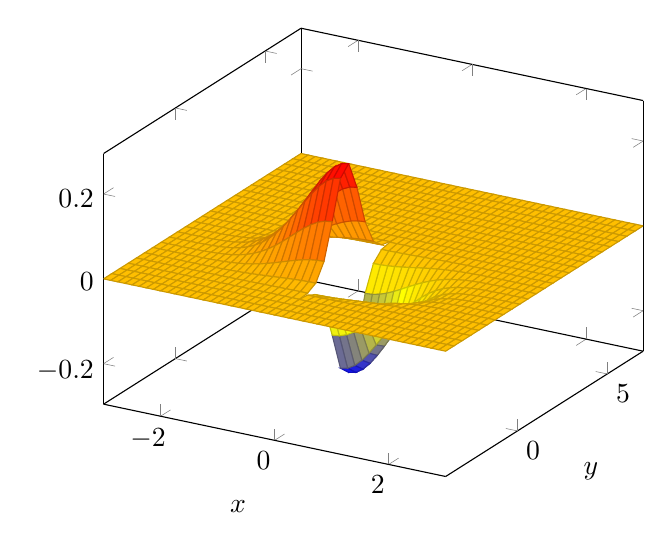
\begin{tikzpicture}
					\begin{axis}[
						view={30}{30},
						xlabel=$x$, ylabel=$y$
					]
					\addplot3[surf, domain =3:0, domain y=-4:7] {-1/4*exp(-x^2-y^2)};
					\addplot3[surf, domain =-3:0, domain y=-4:7] {1/4*exp(-x^2-y^2)};
					\end{axis}
				\end{tikzpicture}
			}
		\end{subfigure}
		\begin{subfigure}{.49\textwidth}
			\centering
			\resizebox{\linewidth}{!}{
				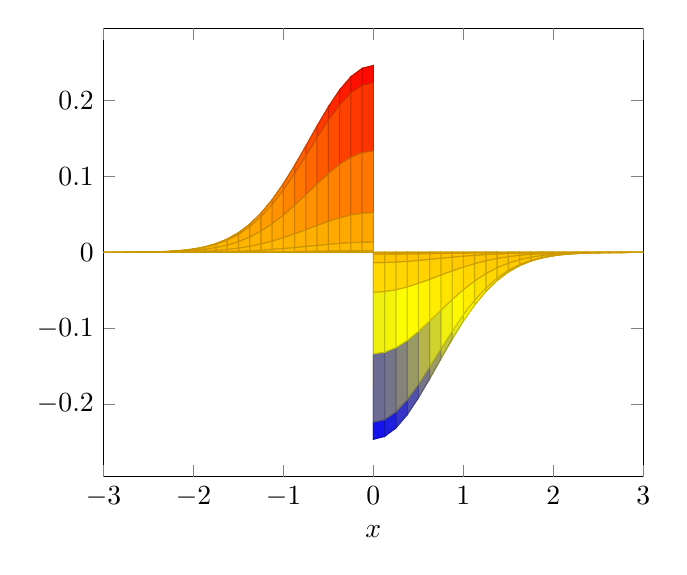
\begin{tikzpicture}
					\begin{axis}[
						view={0}{0},
						xlabel=$x$, ylabel=$y$
					]
					\addplot3[surf, domain =3:0, domain y=-4:7] {-1/4*exp(-x^2-y^2)};
					\addplot3[surf, domain =-3:0, domain y=-4:7] {1/4*exp(-x^2-y^2)};
					\end{axis}
				\end{tikzpicture}
			}
		\end{subfigure}
	\end{figure}
\end{example}
\begin{exercise}
	Sia $f:\R^2 \to \R^m$ derivabile in $x_0$, con $x_0 \in \R^2$. Sia $g:\R^2 \to \R^m$ definita da $g(x,y) = f(y,x)$\\
	Come sono legate le derivate parziali di $f$ e $g$ in $x_0$?
	% TODO solution
\end{exercise}
\begin{exercise}
	Sia $f:A \to \R$ con $A \subseteq \R^n$, derivabile in $x_0 \in \circdot{A}$ . Determinare le derivate parziali in $x_0$ delle funzioni
	\begin{itemize}
		\item $F:A \to \R^2$ definita da $\bigl( f(x), f(x) \bigr)$
		\item $G:A \times A \to \R$ definita da $G(x,y) = f(x) + f(y)$
	\end{itemize}
	% TODO solution
\end{exercise}
\begin{proposition}
	Siano $A \subseteq \R^n$ e $x_0 \in \circdot{A}$. $f$ è \textbf{derivabile parzialmente} rispetto alla $i$\textit{-esima} coordinata se e solo \textbf{se esiste} finito il limite
	\begin{equation}
		\label{eq:deriv_i_esima}
		\lim\limits_{t \to 0} \frac{f(x_1,\:\dotsc\:,x_i+t,\:\dotsc\:,x_n) - f(x_1,\:\dotsc\:,x_i,\:\dotsc\:,x_n)}{t}
	\end{equation}
	\begin{proof}
		Da \fullref{def:deriv_direz}, scegliendo $v = e_i$ della base canonica, si ottiene la \cref{eq:deriv_i_esima}.
	\end{proof}
\end{proposition}
\begin{exercise}
	\label{ex:funz_derivabili}
	Formulare in modo rigoroso e dimostrare:
	\begin{enumerate}
		\item La somma di funzioni parzialmente derivabili è parzialmente derivabile.
		\item La composizione di funzioni parzialmente derivabili è parzialmente derivabile.
		\item Prodotto e rapporto (quando definiti) di funzioni parzialmente derivabili sono funzioni parzialmente derivabili.
	\end{enumerate}
	% TODO solution
\end{exercise}
\begin{example}
	Sia
	\[
		\funcdef{f}{\R^2}{\R^3}{(x,y)}{
			\begin{bmatrix}
				2x + 3y\\
				\sin (xy^2)\\
				e^{xy}
			\end{bmatrix}
		}
	\]
	Allora la funzione $f$ è derivabile parzialmente su tutto $\R^2$. Inoltre
	\[
		\frac{\partial f}{\partial x}(x,y) =
		\begin{bmatrix}
			2\\
			y^2 \: \cos (xy^2)\\
			y e^{xy}
		\end{bmatrix}
		\qquad\qquad
		\frac{\partial f}{\partial y}(x,y) =
		\begin{bmatrix}
			3\\
			2xy \: \cos (xy^2)\\
			x e^{xy}
		\end{bmatrix}
	\]
\end{example}

\begin{proposition}
	Siano $A \subseteq \R^n$, $x_0 \in \circdot{A}$ e $v \in \R^n$ con $v \neq 0$. Sia $f: A \to \R^m$, allora
	\begin{equation*}
		\begin{gathered}
			f \text{ è \textbf{Derivabile} in $x_0$ nella direzione $v$}\\
			\iff\\
			\forall i = 1,\:\dotsc\:,m \quad \text{la \textbf{componente} $f_i$ \textbf{è derivabile} in $x_0$ nella direzione $v$}
		\end{gathered}
	\end{equation*}
	\begin{proof}
		Applicando \fullref{prop:succ_conv_se_comp_conv} e \fullref{prop:cont_e_cont_per_succ}.
		\begin{note}
			Questa è la dimostrazione proposta dal libro, ma non pare davvero sensata. Son accette pull request per integrare...
		\end{note}
		% TODO proper proof. This does not make sense as of now, I know.
	\end{proof}
\end{proposition}
\begin{exercise}
	\label{ex:deriv_non_impl_cont}
	La derivabilità in ogni direzione non implica la continuità. Verificare che la funzione
	\[\funcdef{f}{\R^2}{\R}{(x,y)}
	{
		\begin{cases}
			1 \qquad \text{se } y = x^2 \text{ e } x \neq 0\\
			0 \qquad \text{altrimenti}
		\end{cases}
	}\]
	ammette nell'origine derivate direzionali in ogni direzione ma che \textit{non} è continua nell'origine.
	\begin{figure}[H]
		\begin{subfigure}{.49\textwidth}
			\centering
			\resizebox{\linewidth}{!}{
				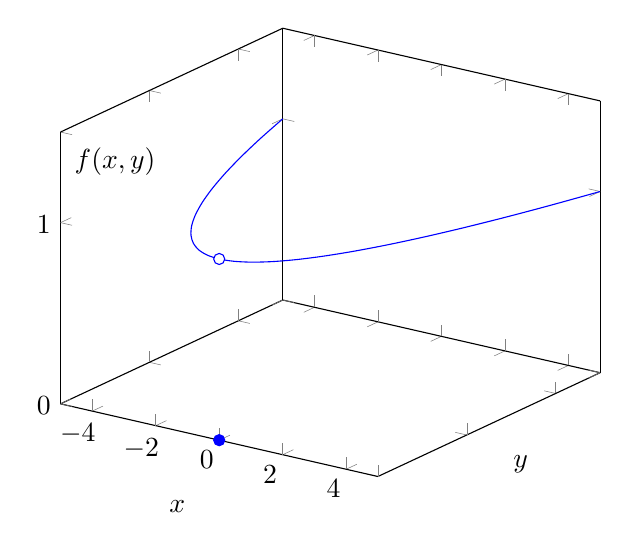
\begin{tikzpicture}
					\begin{axis}[
						xlabel=$x$, ylabel=$y$, zlabel={$f(x,y)$}, zlabel style={rotate=-90},
						% z label placed inside the graph, since on the outside it'd have taken too much horizontal space
						z label style={at={(axis cs: -1.7, 0, 1.5)}},
						yticklabels={,,},
						samples y=0,
						zmin = 0, zmax = 1.5,
						view={35}{25}
					]
					\addplot3 [smooth, color=blue] (x,x^2,1);
					\addplot3 [color=blue, fill=white, only marks,mark=*] coordinates{(0,0,1)};
					\addplot3 [color=blue, only marks, mark=*] coordinates{(0,0,0)};
					\end{axis}
				\end{tikzpicture}
			}
			\caption{Funzione nello spazio}
		\end{subfigure}
		\begin{subfigure}{.49\textwidth}
			\centering
			\resizebox{\linewidth}{!}{
				\begin{tikzpicture}[declare function = {parabola(\x)=\x^2;}]
					\begin{axis} [
						axis lines = center,
						xlabel=$x$, ylabel=$y$,
						xticklabels={,,}, yticklabels={,,},
						ymin = -1
					]
						\addplot[color=blue!70, smooth] {parabola(x)};
				
						\pgfplotsinvokeforeach{-4.4,-3,-2,-1,1,2,3,4.4} {
							\node at (#1, {parabola(#1)}) {$1$};
						}
				
						\node at (0, 0) {$0$};
						\node at (-.4, 2) {$0$};
						\node at (4, 5) {$0$};
						\node at (.6, 8) {$0$};
						\node at (2, 13) {$0$};
						\node at (-2.5, 15) {$0$};
						\node at (-1.5, 18) {$0$};
						\node at (3.5, 20) {$0$};
						\node at (1.3, 22) {$0$};
						\node at (-4, 23) {$0$};
					\end{axis}
				\end{tikzpicture}
			}
			\caption{Valori della $f(x,y)$}
		\end{subfigure}
	\end{figure}

	\begin{solution}
		Le derivate direzionali sono
		\begin{align*}
			\partial_x f(0,0) &= \lim\limits_{t \to 0} \frac{f(0+t,0)-f(0,0)}{t} = 0\\
			\partial_y f(0,0) &= \lim\limits_{t \to 0} \frac{f(0,0+t)-f(0,0)}{t} = 0\\
			D_v f(0,0) &= \lim\limits_{t \to 0} \frac{f(0+t_1,0+t_2)-f(0,0)}{t} = 0
		\end{align*}
		Dunque, per ogni derivata parziale o direzionale in $(0,0)$ il valore della derivata sarà $0$.\\
		D'altro canto $f$ in $0$ \textit{non} è continua in $(0,0)$, quindi si è verificato che la derivabilità non implichi la continuità con $\dim A > 1$
	\end{solution}
\end{exercise}
\begin{exercise}
	Esibire una funzione $f: \R^2 \to \R$ che ammetta in (almeno) un punto una derivata parziale rispetto ad $x$ ma non rispetto a $y$
	\begin{solution}
		La
		\[\funcdef{f}{\R^2}{\R}{(x,y)}{x+\sqrt{y}}\]
		È derivabile parzialmente rispetto a $x$ ma non rispetto a $y$ in $(0,0)$, infatti
		\begin{align*}
			\partial_x f(0,0) &= \lim\limits_{t \to 0} \frac{f(0+t,0)-f(0,0)}{t} = \frac{t-0}{t} = 1\\
			\partial_y f(0,0) &= \lim\limits_{t \to 0} \frac{f(0,0+t)-f(0,0)}{t} = \frac{\sqrt{t}-0}{t} = +\infty \quad \implies \quad \nexists \text{ limite finto}
		\end{align*}
	\end{solution}
\end{exercise}

\newpage
\section{Derivata Totale}
\begin{theorem}[di Lagrange]\leavevmode\vspace*{-\baselineskip}
	\index{Teorema!di Lagrange}
	\label{teo:lagrange}
	\begin{note}
		Questo teorema viene trattato approfonditamente nel corso di Analisi 1 e si applica solo a funzioni $\R^1 \to \R^1$, qui verrà solo riportato rapidamente l'enunciato
	\end{note}
	\begin{note}
		Questo teorema è anche noto come \textit{Teorema del Valor Medio Differenziale}
	\end{note}
	Sia $f: \intervalclose{a}{b} \to \R$ una funzione \textbf{Continua} nell'intervallo chiuso $\intervalclose{a}{b}$ e \textbf{Derivabile} nell'intervallo aperto $\intervalopen{a}{b}$. Allora esiste almeno un punto
	\[c \in \intervalopen{a}{b} : f'(c) = \frac{f(b)-f(a)}{b - a}\]
	O, alternativamente, nella forma
	\[\xi \in \intervalopen{0}{1} : f'(x_0 + \xi h) = \frac{f(x_0 + h)-f(x_0)}{h}\]
\end{theorem}
\begin{definition}[o piccolo]
	\index{o piccolo}
	\label{def:o_piccolo}
	Siano $A \subseteq \R^n$ e $x_0 \in \circdot{A}$. Siano $f,g: A \to \R^m$ due funzioni.
	\[f=o(g) \text{ per } x \to x_0 \qquad \bydef \qquad \lim\limits_{x \to x_0} \frac{\norm{f(x)}}{\norm{g(x)}} = 0\]
	che si legge $f$ è \textbf{o piccolo} di $g$.
	\begin{note}
		Scrivere $f(x) = o(x^k)$ per $x \to 0$ significa che $f = o(g)$ con $g = x^k$
	\end{note}
	\begin{note}
		\hypertarget{note:o_piccolo_to_0}{}
		Con $o(1)$ per $x \to x_0$ si intende una qualunque funzione tendente a $0$ per $x \to x_0$.
	\end{note}
\end{definition}
\begin{exercise}
	Perché son state utilizzate le norme nella \fullref{def:o_piccolo}?
	\begin{solution}
		Perché l'operazione di divisione è sensata solo tra due scalari, non tra vettori.
	\end{solution}
\end{exercise}
\begin{exercise}
	Quali tra le seguenti uguaglianze sono vere? (In tutte, $x \to 0$)
	\begin{align*}
		o(x) &= o(x) + o(x)			&\sqrt{x} &= o(x)	&o(x) &= 10^6 o(x)\\
		o(x^2) &= o(x) \cdot o(x)	&o(x) &= \abs{o(x)}	&x + x^2 &= o(x)\\
		o(x^2) &= o(x) - o(x)		&x &= o(\sqrt{x})	&x &= o(x + x^2)
	\end{align*}
\end{exercise}
\vspace*{\baselineskip}
La seguente definizione è da ritenersi già nota da Analisi 1
\begin{definition}[Derivata in $\R$]
	\index{Derivata!in $\R$}
	Siano $A \subseteq \R$ e $x_0 \in \circdot{A}$. Sia $f: A \to \R$
	\[
		f \text{ \textbf{Derivabile} in } x_0
		\quad \bydef \quad
		\lim\limits_{h \to 0} \frac{f(x_0 + h) - f(x_0)}{h} \text{  esiste finito}
	\]
\end{definition}

\begin{samepage}
Direttamente dalla nozione di Analisi 1 di derivata, si ottiene la seguente relazione tra derivata e coefficiente angolare della retta tangente in un punto
\begin{proposition}
	\label{prop:deriv_analisi_1}
	Siano $A \subseteq \R$ e $x_0 \in \circdot{A}$. Sia $f: A \to \R$
	\begin{equation*}
		\begin{gathered}
			f \text{ \textbf{Derivabile} in } x_0\\
			\iff\\
			\exists m \in \R:\; f(x_0+h) = f(x_0) + mh +o(h) \text{ per } h \to 0
		\end{gathered}
	\end{equation*}
	\begin{proof}
		\begin{align*}
			& f \text{ è derivabile in } x_0\\
			\iff & \lim\limits_{h \to 0} \frac{f(x_0 + h) - f(x_0)}{h} \quad \text{esiste finito}\\
			\iff & \exists m \in \R:\; \lim\limits_{h \to 0} \frac{f(x_0 + h) - f(x_0)}{h} = m\\
			\iff & \exists m \in \R:\; \lim\limits_{h \to 0} \frac{f(x_0 + h) - f(x_0)}{h} - m = 0\\
			\iff & \exists m \in \R:\; \lim\limits_{h \to 0} \frac{f(x_0 + h) - f(x_0) -mh}{h} = 0
			\shortintertext{Per la \hyperlink{note:o_piccolo_to_0}{\notestyle{} 2 alla \fullref*{def:o_piccolo}}}
			\iff & \exists m \in \R:\; f(x_0 + h) - f(x_0) -mh = o(h) \text{ per } h \to 0\\
			\iff & \exists m \in \R:\; f(x_0 + h) = f(x_0) -mh + o(h) \text{ per } h \to 0
		\end{align*}
	\end{proof}
\end{proposition}
\end{samepage}

\noindent Analogamente a quanto fatto nella \fullref{prop:deriv_analisi_1}, si definisce
\begin{definition}[Differenziale]
	\index{Differenziale}
	\index{Derivata!Totale}
	\index{Funzione!Differenziabile}
	\label{def:differenz}
	Siano $A \subseteq \R^n$ e $x_0 \in \circdot{A}$. Sia $f: A \to \R^m$
	\begin{equation*}
		\begin{gathered}
			f \text{ è \textbf{Differenziabile} in } x_0\\
			\bydef\\
			\exists M \in \mat (m \times n):\; f(x_0 + h) = f(x_0) + Mh + o(h) \text{ per } h \to 0
		\end{gathered}
	\end{equation*}
	La matrice $M$ è la \textbf{Derivata Totale} di $f$ calcolata in $x_0$ e si indica con $Df(x_0)$. $Df(x_0)$ è l'applicazione \textit{lineare} che meglio approssima la variazione di $f$ nelle vicinanze di $x_0$.
	\begin{note}
		Verrà spiegato più avanti in \fullref{coro:se_diff_deriv_parz} un metodo pratico di calcolo della Derivata Totale.
	\end{note}
\end{definition}
\begin{observation}[Matrici Derivata Totale Particolari]
	\index{Matrice!Jacobiana}
	\index{Gradiente}
	\index{Vettore Tangente}
	\label{obs:matr_deriv_tot}
	Data la matrice $Df(x_0)$ con $m$ righe e $n$ colonne:
	\begin{itemize}
		\item Se $n = 1$ e $m = 1$ $Df(x_0)$ è \textbf{Derivata} di Analisi 1, uno scalare
		\item Se $n > 1$ e $m = 1$ $Df(x_0)$ è \textbf{Gradiente} di $f$ e si indica con $\nabla f(x_0)$ (\textit{nabla} $f$) o $\grad f(x_0)$
		\item Se $n = 1$ e $m > 1$ $Df(x_0)$ è \textbf{Vettore Tangente} alla $f$
		\item Se $n > 1$ e $m > 1$ $Df(x_0)$ è \textbf{Matrice Jacobiana} di $f$ e si può anche indicare con $J_f(x_0)$
	\end{itemize}
	Come si vedrà in \fullref{coro:se_diff_deriv_parz}, il Gradiente della \textit{i-esima} variabile è la \textit{i-esima} colonna di $Df(x_0)$. Il Vettore Tangente della \textit{j-esima} variabile è invece la \textit{j-esima} riga di $Df(x_0)$.\\
	Si veda \fullref{ex:Df_e_deriv_parz} per alcuni esempi di $Df$ con diverse forme.
\end{observation}
\begin{exercise}
	Perché non è stata data una definizione di derivata attraverso il limite del rapporto incrementale?
	% TODO solution
\end{exercise}
\begin{example}
	Siano $M \in \mat(m \times n)$ una matrice fissata, $f: \R^n \to \R^m$ data da $f(x) = Mx$.\\
	Allora $f$ è differenziabile ovunque e per ogni $x_0 \in \R$ si ha $Df(x_0) = M$
\end{example}
\begin{proposition}[Unicità della Derivata Totale]
	\index{Unicità!Derivata Totale}
	\label{prop:unic_deriv_tot}
	Siano $A \subseteq \R^n$, $x_0 \in \circdot{A}$, $f: A \to \R^m$ e $M_1, M_2 \in \mat(m \times n)$
	\begin{equation*}
		\left.
		\begin{array}{l}
			M_1 \text{ derivata totale di } f \text{ in } x_0\\
			M_2 \text{ derivata totale di } f \text{ in } x_0
		\end{array}
		\right\}
		\quad \implies \quad
		M_1 = M_2
	\end{equation*}
	\begin{proof}
		Sia $t \in \R$ e sia fissato un vettore $e_i$ della base canonica di $\R^n$. Il \textit{prodotto per scalare} $e_i t$ è ancora un vettore in $\R^n$ con l'$i$-esima componente uguale a $t$.
		\begin{align*}
			\shortintertext{Si esegua ora}
			M_2 e_i - M_1 e_1 &=
			\shortintertext{Moltiplicando e dividendo per $t$}
			&= \frac{1}{t} M_2 (e_i t) - \frac{1}{t} M_1 (e_i t)
			\shortintertext{Grazie alla \fullref{def:differenz}}
			&= \frac{1}{t} [f(x_0 + t e_i) - f(x_0) + o(t)] - \frac{1}{t} [f(x_0 + t e_i) - f(x_0) + o(t)]\\
			&= \frac{1}{t} o(t) \text{ per } t \to 0
		\end{align*}
		Essendo stato lasciato $e_i$ generico, significa che è possibile applicare questo ragionamento ad uno qualsiasi degli $n$ vettori della base canonica. Quindi è possibile confrontare tra loro tutte le $n$ colonne delle $M_1$ e $M_2$, verificando l'uguaglianza delle matrici e, quindi, delle due applicazioni lineari.
	\end{proof}
\end{proposition}
\begin{proposition}
	Siano $A \subseteq \R^n$, $x_0 \in \circdot{A}$ e $f:A \to \R^m$
	\[
		f \text{ \textbf{Differenziabile} in } x_0
		\quad \implies \quad
		f \text{ \textbf{Continua} in } x_0
	\]
	\begin{proof}
		Per ipotesi $x_0 \in \circdot{A}$, dunque $x_0$ è di accumulazione. A questo punto, grazie alla \fullref{prop:f_cont_se_isol_o_accum} basta verificare che $\lim\limits_{x \to x_0} f(x) = f(x_0)$. Dalla \fullref{def:differenz}
		\[f(x_0 + h) = f(x_0) + Mh + o(h) \text{ per } h \to 0\]
		Quindi, posto $h = x - x_0$ ed essendo $M = Df(x_0)$ per \fullref{def:differenz}
		\[\lim\limits_{x \to x_0} f(x) = \lim\limits_{x \to x_0} \bigl[f(x_0) + Df(x_0)(x-x_0) + o(x - x_0)\bigr] = f(x_0)\]
	\end{proof}
\end{proposition}
\begin{proposition}
	\label{prop:se_diff_deriv_dir}
	Siano $A \subseteq \R^n$, $x_0 \in \circdot{A}$ e $f:A \to \R^m$
	\[
		f \text{ \textbf{Differenziabile} in } x_0
		\quad \implies \quad
		\begin{cases}
			\begin{array}{c}
				f \text{ ammette ogni \textbf{Derivata Direzionale} in } x_0\\
				e\\
				\forall v \in \R^n \setminus \brackets{0} \quad D_v f(x_0) = Df(x_0)v
			\end{array}
		\end{cases}
	\]
	\begin{proof}
		Sia $v \in \R^n$ non nullo. Partendo dalla \fullref{def:deriv_direz}
		\begin{align*}
			&\lim\limits_{t \to 0} \frac{f(x_0 + tv) - f(x_0)}{t}
			\shortintertext{Sostituendo ora $f(x_0 + tv)$ con il secondo membro della \fullref{def:differenz}, dopo aver posto $h = tv$}
			= &\lim\limits_{t \to 0} \frac{f(x_0) + Df(x_0)(tv) + o(tv) - f(x_0)}{t}\\
			= &\lim\limits_{t \to 0} \frac{Df(x_0)(tv)}{t} + \lim\limits_{t \to 0} \frac{o(tv)}{t}\\
			= &Df(x_0)v
		\end{align*}
	\end{proof}
\end{proposition}
\begin{corollary}
	\label{coro:se_diff_deriv_parz}
	Siano $A \subseteq \R^n$, $x_0 \in \circdot{A}$ e $f:A \to \R^m$
	\[
		f \text{ \textbf{Differenziabile} in } x_0
		\quad \implies \quad
		\begin{cases}
			\begin{array}{c}
				f \text{ ammette ogni \textbf{Derivata Parziale} in } x_0\\
				e\\
				\frac{\partial f}{\partial x_i}(x_0) = Df(x_0) \cdot e_i
			\end{array}
		\end{cases}
	\]
	Dove $Df(x_0) \cdot e_i$ non è altro che
	\[
		Df(x_0) \cdot e_i =
		\begin{bmatrix}
			x_{11} & \cdots & x_{1i} & \cdots & x_{1n}\\
			x_{21} & \cdots & x_{2i} & \cdots & x_{2n}\\
			\vdots & \vdots & \vdots & \ddots & \vdots\\
			x_{n1} & \cdots & x_{ni} & \cdots & x_{nn}\\
		\end{bmatrix}
		\cdot
		\begin{bmatrix}
			(0 & \dots & 1 & \dots & 0)
		\end{bmatrix}
		=
		\begin{bmatrix}
			0 & \cdots & x_{1i} & \cdots & 0\\
			0 & \cdots & x_{2i} & \cdots & 0\\
			\vdots & \vdots & \vdots & \ddots & \vdots\\
			0 & \cdots & x_{ni} & \cdots & 0\\
		\end{bmatrix}
	\]
	Cioè l'\textit{i-esima} colonna della $Df(x_0)$, come da \fullref{obs:matr_deriv_tot}
	\begin{note}
		Per quanto detto, il presente corollario offre il principale metodo di calcolo della \textbf{Derivata Totale}\\
		Inoltre è anche una dimostrazione alternativa della \fullref{prop:unic_deriv_tot}
	\end{note}
	\begin{proof}
		Direttamente dalla \fullref{prop:se_diff_deriv_dir} e dalla \fullref{def:deriv_parz}.
	\end{proof}
\end{corollary}
\begin{example}
	\label{ex:Df_e_deriv_parz}
	Esempi relazioni tra Derivata Totale e derivate parziali
	\begin{align*}
		n = 2 \quad m = 1 \qquad & Df =
		\begin{bmatrix}
			\frac{\partial f}{\partial x} & \frac{\partial f}{\partial y}
		\end{bmatrix}\\
		n = 3 \quad m = 1 \qquad & Df =
		\begin{bmatrix}
			\frac{\partial f}{\partial x} & \frac{\partial f}{\partial y} &  \frac{\partial f}{\partial z}
		\end{bmatrix}\\
		n = 1 \quad m = 2 \qquad & Df =
		\begin{bmatrix}
			\frac{\partial f_1}{\partial x}\\[1ex]
			\frac{\partial f_2}{\partial x}
		\end{bmatrix}\\
		n = 2 \quad m = 2 \qquad & Df =
		\begin{bmatrix}
			\frac{\partial f_1}{\partial x} & \frac{\partial f_1}{\partial y}\\[1ex]
			\frac{\partial f_2}{\partial x} & \frac{\partial f_2}{\partial y}
		\end{bmatrix}\\
		n > 2 \quad m > 2 \qquad & Df =
		\begin{bmatrix}
			\frac{\partial f_1}{\partial x_1} & \frac{\partial f_1}{\partial x_2} & \dots & \frac{\partial f_1}{\partial x_n}\\[1ex]
			\frac{\partial f_2}{\partial x_1} & \frac{\partial f_2}{\partial x_2} & \dots & \frac{\partial f_2}{\partial x_n}\\[1ex]
			\vdots & \vdots & \ddots & \vdots\\[1ex]
			\frac{\partial f_m}{\partial x_1} & \frac{\partial f_m}{\partial x_2} & \dots & \frac{\partial f_m}{\partial x_n}
		\end{bmatrix}
	\end{align*}
\end{example}
\begin{observation}
	Sia \fullref{prop:se_diff_deriv_dir} che \fullref{coro:se_diff_deriv_parz} non possono essere invertiti, come verificato in \fullref{ex:deriv_non_impl_cont}.
\end{observation}
\begin{corollary}
	Siano $A \subseteq \R^n$, $x_0 \in \circdot{A}$ e $f:A \to \R^m$
	\[
		f \text{ \textbf{Differenziabile} in } x_0
		\quad \implies \quad
		f \text{ \textbf{Derivabile} in } x_0
	\]
	\begin{proof}
		Mediante il \fullref{coro:se_diff_deriv_parz} si vede immediatamente che rispetta la \fullref{def:deriv_parz}.
	\end{proof}
\end{corollary}
\begin{corollary}
	\label{coro:f_diff_con_matr_comp}
	Siano $A \subseteq \R^n$, $x_0 \in \circdot{A}$ e $f:A \to \R^m$. Sia $f$ derivabile parzialmente in $x_0$ e sia $M$ la $Df(x_0)$, matrice dei coefficienti $M_{ij} = \frac{\partial f_i}{\partial x_j}$
	\begin{equation*}
		\begin{gathered}
			f \text{ \textbf{Differenziabile} in } x_0\\
			\iff\\
			f(x_0 + h) - f(x_0) - Mh = o(h) \text{ per } h \to 0
		\end{gathered}
	\end{equation*}
	\begin{note}
		Questo corollario formalizza la relazione tra le Derivate Parziali e la Matrice Derivata Totale $M$
	\end{note}
	\begin{proof}
		Direttamente dalla \fullref{def:differenz}, per mezzo del \fullref{coro:se_diff_deriv_parz}.
	\end{proof}
\end{corollary}
\begin{exercise}
	Verificare che, nel caso $n = 2$ ed $m = 1$ il \fullref{coro:f_diff_con_matr_comp} si scrive
	\begin{equation*}
		\begin{gathered}
			f \text{ \textbf{Differenziabile} in } x_0\\
			\iff\\
			f(x_0 + h, y_o + k) - f(x_0, y_0) -
			\begin{bmatrix}
				\frac{\partial f}{\partial x}(x_0, y_0) & \frac{\partial f}{\partial y}(x_0, y_0)
			\end{bmatrix}
			\cdot
			\begin{bmatrix}
				h\\
				k
			\end{bmatrix}
			= o(\sqrt{h^2 + k^2}) \text{ per } h, k \to 0
		\end{gathered}
	\end{equation*}
	% TODO solution
\end{exercise}
\begin{exercise}
	Scrivere il \fullref{coro:f_diff_con_matr_comp} nel caso $n = 3$ ed $m = 1$
	% TODO solution
\end{exercise}

\begin{theorem}[del Differenziale Totale]
	\index{Teorema!del Differenziale Totale}
	\label{teo:diff_tot}
	Siano $A \subseteq \R^n$, $x_0 \in \circdot{A}$ e $f:A \to \R^m$.
	\[
		\left.
			\begin{array}{c}
				\text{Per } i = 1,\:\dotsc\:,m \text{ e } j = 1,\:\dotsc\:,n\\
				\dfrac{\partial f_i}{\partial x_j} \text{ è \textbf{definita} in un intorno di } x_0 \text{ e  \textbf{Continua} in } x_0
			\end{array}
		\right\}
		\quad \implies \quad
		f \text{ è \textbf{Differenziabile} in } x_0
	\]
	Cioè la verifica della Differenziabilità in un punto può essere ricondotta alla verifica di esistenza e continuità delle Derivate Parziali.
	\begin{proof}
		Si può supporre $n = 2$ e $m = 1$ in quanto il caso più generale è del tutto analogo.\\
		È necessario verificare la \fullref{def:differenz}, dunque in $\R^n = \R^2$ si ha
		\begin{equation}
			\label{eq:deriv_tot_def_diff}
			f(x_0 + h, y_0 + k) = f(x_0, y_0) + Df(x_0, y_0) \begin{bmatrix}h\\k\end{bmatrix} + o(h,k) \text{ per } h,k \to 0
		\end{equation}
		\[f(x_0 + h, y_0 + k) - f(x_0, y_0) = Df(x_0, y_0) \begin{bmatrix}h\\k\end{bmatrix} + o(h,k) \text{ per } h,k \to 0\]
		Preso in considerazione solo il primo membro, si aggiunge e sottrae ad esso la stessa quantità, ottenendo
		\begin{equation}
			\label{eq:teo_diff_tot_sommo_sottraggo}
			f(x_0 + h, y_0 + k) - f(x_0, y_0) = \underbrace{f(x_0 + h, y_0 + k) - f(x_0+h,y_0)}_{\text{(1)}} + \underbrace{f(x_0+h,y_0) - f(x_0, y_0)}_{\text{(2)}}
		\end{equation}
		Considerando la (1) e la (2) di \cref{eq:teo_diff_tot_sommo_sottraggo} come funzioni in una sola variabile, si può applicare il \fullref{teo:lagrange}, grazie alla continuità per ipotesi delle derivate parziali:
		\begin{itemize}
			\item La (1) rispetto a $y$, con $x_0 + h$ fissato
			\item La (2) rispetto a $x$, con $y_0$ fissato
		\end{itemize}
		Spostandosi lungo le direzioni parallele agli assi è possibile andare da $(x_0 + h, y_0 + k)$ a $(x_0, y_0)$
		\begin{center}
			\begin{tikzpicture}
				\pgfmathsetmacro\MAX{8}
				\pgfmathsetmacro\XZ{\MAX / 3 }
				\pgfmathsetmacro\YZ{\MAX / 3 }
				\pgfmathsetmacro\XZh{\MAX / 3 *2}
				\pgfmathsetmacro\YZk{\MAX / 3 *2}
				\coordinate (X0Y0) at (\XZ,\YZ);
				\coordinate (X0hY0) at (\XZh,\YZ);
				\coordinate (X0Y0k) at (\XZ,\YZk);
				\coordinate (X0hY0k) at (\XZh,\YZk);

				\draw[->] (0,0) -- (\MAX,0) node[anchor=north west] {$x$};
				\draw[->] (0,0) -- (0,\MAX) node[anchor=south east] {$y$};
				\draw[dotted] (\XZ,0) -- (\XZ,\MAX);
				\draw[dotted] (0,\YZ) -- (\MAX,\YZ);
				\draw[dotted] (\XZh,0) -- (\XZh,\MAX);
				\draw[dotted] (0,\YZk) -- (\MAX,\YZk);
				\draw node[anchor=north] at (\XZ,0) {$x_0$};
				\draw node[anchor=north] at (\XZh,0) {$x_0+h$};
				\draw node[anchor=east] at (0,\YZ) {$y_0$};
				\draw node[anchor=east] at (0,\YZk) {$y_0+k$};
				\draw node at (X0Y0) {$\bullet$};
				\draw node at (X0Y0k) {$\bullet$};
				\draw node at (X0hY0) {$\bullet$};
				\draw node at (X0hY0k) {$\bullet$};
				\draw node[anchor=north east] at (X0Y0) {$(x_0,y_0)$};
				\draw node[anchor=south east] at (X0Y0k) {$(x_0,y_0+k)$};
				\draw node[anchor=north west] at (X0hY0) {$(x_0+h,y_0)$};
				\draw node[anchor=south west] at (X0hY0k) {$(x_0+h,y_0+k)$};

				\draw[<-] (\XZ,\MAX*4/10) -- (\XZ,\MAX*6/10);
				\draw[<-] (\XZh,\MAX*4/10) -- (\XZh,\MAX*6/10);
				\draw[<-] (\MAX*4/10,\YZ) -- (\MAX*6/10,\YZ);
				\draw[<-] (\MAX*4/10,\YZk) -- (\MAX*6/10,\YZk);
			\end{tikzpicture}
		\end{center}
		Quindi, applicando il \fullref{teo:lagrange}:
		\[
			\exists \alpha, \beta \in \intervalopen{0}{1} \textbf{ per cui} \qquad
			\begin{array}{rrcl}
				\text{(1)} & f(x_0 + h, y_0 + k) - f(x_0 + h, y_0) &=& \frac{\partial f}{\partial y} (x_0 + h, y_0 + \beta k) k\\[1ex]
				\text{(2)} & f(x_0 + h, y_0) - f(x_0, y_0) &=& \frac{\partial f}{\partial x} (x_0 + \alpha h, y_0) h
			\end{array}
		\]
		Tornando alla \cref{eq:deriv_tot_def_diff}, si ottiene
		\begin{align*}
			&f(x_0 + h, y_0 + k) - f(x_0, y_0) - Df(x_0, y_0) \begin{bmatrix}h\\k\end{bmatrix}\\
			= &\underbrace{f(x_0 + h, y_0 + k) - f(x_0+h,y_0)}_{\text{(1)}} + \underbrace{f(x_0+h,y_0) - f(x_0, y_0)}_{\text{(2)}} - Df(x_0, y_0) \begin{bmatrix}h\\k\end{bmatrix}\\
			= &\underbrace{\frac{\partial f}{\partial y} (x_0 + h, y_0 + \beta k) k}_{\text{(1)}} + \underbrace{\frac{\partial f}{\partial x} (x_0 + \alpha h, y_0) h}_{\text{(2)}} - Df(x_0, y_0) \begin{bmatrix}h\\k\end{bmatrix}
			\shortintertext{Si esegue il prodotto tra matrice Derivata Totale e vettore incremento $\begin{bmatrix}h\\k\end{bmatrix}$, infine si separano i termini}
			= &	\left( \frac{\partial f}{\partial y} (x_0 + h, y_0 + \beta k) - \frac{\partial f}{\partial y} (x_0 + h, y_0) \right) k +
				\left( \frac{\partial f}{\partial x} (x_0 + \alpha h, y_0) - \frac{\partial f}{\partial x} (x_0, y_0)\right) h
		\end{align*}
		Si passa dunque alla norma
		\begin{gather*}
			\norm{f(x_0 + h, y_0 + k) - f(x_0, y_0) - Df(x_0, y_0) \begin{bmatrix}h\\k\end{bmatrix}}\\
			\shortintertext{Separando come fatto prima ed applicando la disguguaglianza triangolare}
			\leq 	\norm{\left( \frac{\partial f}{\partial y} (x_0 + h, y_0 + \beta k) - \frac{\partial f}{\partial y} (x_0 + h, y_0) \right) k} +
					\norm{\left( \frac{\partial f}{\partial x} (x_0 + \alpha h, y_0) - \frac{\partial f}{\partial x} (x_0, y_0)\right) h}
			\shortintertext{Per proprietà \ref{itm:def_norm_propr_lambda} da \fullref{def:norma}}
			=  \norm{\frac{\partial f}{\partial y} (x_0 + h, y_0 + \beta k) - \frac{\partial f}{\partial y} (x_0 + h, y_0)} \abs{k} +
				\norm{\frac{\partial f}{\partial x} (x_0 + \alpha h, y_0) - \frac{\partial f}{\partial x} (x_0, y_0)} \abs{h}
			\shortintertext{Presa ora la norma del vettore $(h,k)$, cioè $\norm{(h,k)} = \sqrt{h^2 + k^2}$, sicuramente $\abs{h} \leq \norm{(h,k)}$ e $\abs{k} \leq \norm{(h,k)}$, dunque}
			\leq 	\norm{\frac{\partial f}{\partial y} (x_0 + h, y_0 + \beta k) - \frac{\partial f}{\partial y} (x_0 + h, y_0)} \sqrt{h^2 + k^2} +
					\norm{\frac{\partial f}{\partial x} (x_0 + \alpha h, y_0) - \frac{\partial f}{\partial x} (x_0, y_0)} \sqrt{h^2 + k^2}
			\shortintertext{Essendo $h,k \to 0$ da \cref{eq:deriv_tot_def_diff} e graze alla continuità delle derivate, le due norme tendono a $0$. Inoltre, per \fullref{def:o_piccolo}}
			=\; o(1) \sqrt{h^2 + k^2} \text{ per } \begin{bmatrix}h\\k\end{bmatrix} \to 0\\
			=\; o(\sqrt{h^2 + k^2}) \text{ per } \begin{bmatrix}h\\k\end{bmatrix} \to 0
		\end{gather*}
		Da cui la tesi, avendo verificato la \fullref{def:differenz}.
	\end{proof}
\end{theorem}
\begin{exercise}
	Data la funzione
	\[
		\funcdef{f}{\R}{\R}{x}{
			\begin{cases}
				\begin{array}{ll}
					x^2 \sin \frac{1}{x} & x \neq 0\\
					0 & x = 0
				\end{array}
			\end{cases}
		}
	\]
	Verificare che $f$ è differenziabile su $\R$ ma non ha derivata continua su $\R$.
	% TODO solution
\end{exercise}

\begin{definition}[Funzioni di Classe $\cntclass{1}$]
	\index{Classe!$\cntclass{1}$}
	\label{def:cnt_class_1}
	Sia $A \subseteq \R^n$ un \textbf{Aperto}.
	\begin{center}
		$\cntclass{1}(A; \R^m)$ è l'insieme delle funzioni $f:\; A \to \R^m$\\
		con \textbf{tutte} le \textbf{Derivate Parziali prime continue} in ogni punto di $A$
	\end{center}
	Si legge \textit{$f$ è di classe $\cntclass{1}$ su $A$ con valori in $\R^m$}.
\end{definition}
\begin{observation}
	Si ricorda la \fullref{prop:convesso_deriv_par_lim_allora_lips} che è attinente anche a questo capitolo.
\end{observation}
\begin{corollary}
	Sia $A \subseteq \R^n$ un \textbf{Aperto}. Se $f \in \cntclass{1}(A;\R^m)$ allora $f$ è \textbf{Differenziabile} su $A$.
	\begin{proof}
		Applicare il \fullref{teo:diff_tot}.
	\end{proof}
\end{corollary}
\begin{proposition}
	\label{prop:cnt_class_components}
	Siano $m \in \N, m \geq 1$ e $A \subseteq \R^n$ un \textbf{Aperto}
	\[f \in \cntclass{1}(A; \R^m) \iff \forall i = 1,\:\dotsc\:, m \quad f_i \in \cntclass{1}(A;\R)\]
	\begin{proof}
		Immediata.
	\end{proof}
\end{proposition}
\begin{exercise}
	Dimostrare la \fullref{prop:cnt_class_components}.
	% TODO solution
\end{exercise}
\begin{exercise}
	Dimostrare che $\cntclass{1}(A;\R)$ non coincide con l'insieme delle funzioni differenziabili su $A$ con valori in $\R$.
	% TODO solution
\end{exercise}

\subsection{Regole di Derivazione}\label{sect:regole_deriv}
\begin{note}
	In questa sezione per forme tipo $(f + g)(x_0)$ oppure $(f \cdot g)(x_0)$ si intendono, ad esempio, la somma o il prodotto delle due funzioni nel punto $x_0$, quindi $f(x_0) + g(x_0)$ e così via.
\end{note}
\begin{proposition}[Differenziale del Prodotto per Scalare]
	\index{Differenziale!Prodotto per Scalare}
	Siano $A \subseteq \R^n$ un \textbf{Aperto}, $x_0 \in A$, $f:\; A \to \R^m$ e $\lambda \in \R$, allora
	\[
		f \text{ \textbf{Differenziabile} in } x_0
		\quad \implies \quad
		\begin{cases}
			\begin{array}{c}
				\lambda f \text{ \textbf{Differenziabile} in } x_0\\
				e\\
				D(\lambda f)(x_0) = \lambda Df(x_0)
			\end{array}
		\end{cases}
	\]
	\begin{proof}
		Essendo $f$ differenziabile per ipotesi, si ha
		\[f(x_0 + h) = f(x_0) + Df(x_0)h + o(h)\]
		Dunque, considerando la $\lambda f$
		\[(\lambda f)(x_0 + h) = (\lambda f)(x_0) + \lambda Df(x_0)h + o(h)\]
		Che è la \fullref{def:differenz} per $\lambda f(x_0)$, da cui la tesi.
	\end{proof}
\end{proposition}
\begin{proposition}[Differenziale della Somma di Funzioni]
	\index{Differenziale!Somma di Funzioni}
	\label{prop:diff_somma_funz}
	Siano $A \subseteq \R^n$ un \textbf{Aperto}, $x_0 \in A$, $f, g:\; A \to \R^m$, allora
	\[
		\left.
		\begin{array}{c}
			f \text{ \textbf{Differenziabile} in } x_0\\
			g \text{ \textbf{Differenziabile} in } x_0
		\end{array}
		\right\}
		\quad \implies \quad
		\begin{cases}
			\begin{array}{c}
				f + g \text{ \textbf{Differenziabile} in } x_0\\
				e\\
				D(f + g)(x_0) = Df(x_0) + Dg(x_0)
			\end{array}
		\end{cases}
	\]
	\begin{proof}
		Essendo $f$ e $g$ differenziabili per ipotesi si hanno
		\begin{align*}
			f(x_0 + h) &= f(x_0) + Df(x_0)h + o(h)\\
			g(x_0 + h) &= g(x_0) + Dg(x_0)h + o(h)
		\end{align*}
		Dunque, sommando membro a membro si arriva alla
		\begin{align*}
			f(x_0 + h) + g(x_0 + h) &= f(x_0) + g(x_0) + Df(x_0)h + Dg(x_0)h + o(h)\\
			(f + g)(x_0 + h) &= (f + g)(x_0) + \bigl( Df(x_0) + Dg(x_0) \bigr) h + o(h)
		\end{align*}
		Che è la \fullref{def:differenz} per $(f + g)(x_0)$, da cui la tesi.
	\end{proof}
\end{proposition}
\begin{proposition}[Differenziale del Prodotto Scalare]
	\index{Differenziale!Prodotto Scalare}
	\label{prop:diff_prod_scal}
	Siano $A \subseteq \R^n$ un \textbf{Aperto}, $x_0 \in A$, $f, g:\; A \to \R^m$, allora
	\[
		\left.
		\begin{array}{c}
			f \text{ \textbf{Differenziabile} in } x_0\\
			g \text{ \textbf{Differenziabile} in } x_0
		\end{array}
		\right\}
		\quad \implies \quad
		\begin{cases}
			\begin{array}{c}
				f \cdot g \text{ \textbf{Differenziabile} in } x_0\\
				e\\
				D(f \cdot g)(x_0) = g(x_0)^T \; Df(x_0) + f(x_0)^T \; Dg(x_0)
			\end{array}
		\end{cases}
	\]
	\vspace*{-\baselineskip}
	\begin{note}
		$\;\cdot\;$ indica il \textbf{Prodotto Scalare} tra vettori che può essere scritto in forma matriciale con $f^T g$ (dunque utilizzando il prodotto righe per colonne) dove $f^T$ è la matrice \textbf{Trasposta} di $f$.
	\end{note}
	\begin{proof}
		Omessa in aula.

		\cbstart
		\noindent Utilizzando la differenziabilità di $f$ e $g$ assieme alla continuità di $g$
		\begin{align*}
			\lefteqn{(f \cdot g)(x_0 + h) - (f \cdot g)(x_0) =}\\
			&= (f^T\;g)(x_0 + h) - (f^T\;g)(x_0)\\
			&= \bigl( f(x_0 + h) - f(x_0) \bigr)^T g(x_0 + h) + f(x_0)^T \bigl( g(x_0 + h) - g(x_0) \bigr)\\
			&= \bigl( Df(x_0)h + o(h) \bigr)^T \bigl( f(x_0) + o(1) \bigr) + f(x_0)^T \bigl( Dg(x_0)h + o(h) \bigr)\\
			&= \bigl( Df(x_0)h \bigr)^T g(x_0) + f(x_0)^T \bigl( Dg(x_0) h \bigr) + o(h)\\
			&= h^T Df(x_0)^T g(x_0) + f(x_0)^T Dg(x_0)h + o(h)\\
			&= \bigl( g(x_0)^T Df(x_0) + f(x_0)^T Dg(x_0) \bigr) h + o(h)
		\end{align*}
		da cui la tesi per la \fullref{def:differenz}.
		\cbend
	\end{proof}
\end{proposition}
\begin{exercise}
	Verificare che gli ordini delle matrici sono tali da permettere le operazioni eseguite nella \fullref{prop:diff_prod_scal}.
	% TODO solution
\end{exercise}
\begin{exercise}
	Scrivere la \fullref{prop:diff_prod_scal} nel caso $m = 1$ utilizzando i vettori $\nabla f$ e $\nabla g$.
	% TODO solution
\end{exercise}
\begin{exercise}
	Siano $A \subseteq \R^n$ un \textbf{Aperto}, $x_0 \in A$, $f:\; A \to \R$ e $g:\; A \mapsto \R^m$ entrambe \textbf{Differenziabili} in $x_0$.\\
	Dimostrare che $f \; g$ (prodotto di funzione scalare per funzione vettoriale) è \textbf{Differenziabile} in $x_0$ e determinarne la derivata totale.
	% TODO solution
\end{exercise}
\begin{exercise}
	Siano $A \subseteq \R^n$ un \textbf{Aperto}, $x_0 \in A$, $f:\; A \to \R^m$ e $g:\; A \mapsto \R^p$ entrambe \textbf{Differenziabili} in $x_0$. Sia ora
	\[
		\funcdef{
			F
		}{
			A
		}{
			\R^{m + p}
		}{
			x
		}{
			\bigl( f(x), g(x) \bigr)
		}
	\]
	Dimostrare che $F$ è \textbf{Differenziabile} in $x_0$ e determinarne la derivata totale.
	% TODO solution
\end{exercise}
\begin{exercise}
	Siano $A \subseteq \R^n$ un \textbf{Aperto}, $x_0 \in A$ e $f,g:\; A \to \R^3$ entrambe \textbf{Differenziabili} in $x_0$.\\
	Dimostrare che il prodotto vettoriale $f \wedge g$ è \textbf{Differenziabile} in $x_0$ e determinarne la derivata totale.
	% TODO solution
\end{exercise}

\begin{proposition}[Differenziale della Funzione Composta]
	\index{Differenziale!Funzione Composta}
	\label{prop:diff_funz_comp}
	Siano:
	\begin{itemize}[noitemsep]
		\item $A \subseteq \R^n$
		\item $g:\; A \to \R^m$
		\item $B \subseteq \R^m$
		\item $f:\; B \to \R^p$
		\item $x_0 \in \circdot{A}$ tale che $g(x_0) \in \circdot{B}$
		\item $g$ \textbf{Differenziabile} in $x_0$
		\item $f$ \textbf{Differenziabile} in $g(x_0)$
	\end{itemize}
	Allora
	\[
		\begin{gathered}
			f \circ g \text{ è \textbf{Differenziabile} in } x_0\\
			e\\
			D(f \circ g)(x_0) = Df \bigl( g(x_0) \bigr) Dg(x_0)
		\end{gathered}
	\]
	\begin{note}
		$(f \circ g)(x_0) = f \bigl( g(x_0) \bigr)$
	\end{note}
	\begin{note}
		In questa proposizione, a differenza delle altre del capitolo, non è richiesta l'apertura di $A$, ma piuttosto che $x_0$ appartenga alla \textbf{Parte Interna} di $A$, $\circdot{A}$. Concettualmente è la stessa cosa, ma sarebbe risultato meno evidente il fatto che anche $g(x_0)$ debba essere nella \textbf{Parte Interna} di $B$, $\circdot{B}$.\\
		Le ipotesi avrebbero comunque potuto essere formulate come $A$ e $B$ \textbf{Aperti}.
	\end{note}
	\begin{proof}
		Essendo $g(x)$ e $f\bigl( g(x) \bigr)$ differenziabili per ipotesi si hanno
		\begin{equation}
			\label{eq:diff_somma_funz_Dg}
			g(x_0 + h) = g(x_0) + Dg(x_0)h + o(h) \quad \text{per } h \to 0
		\end{equation}
		\begin{equation}
			\label{eq:diff_somma_funz_Df}
			f\bigl( g(x_0) + k \bigr) = f\bigl( g(x_0) \bigr) + Df\bigl( g(x_0) \bigr)k + o(k) \quad \text{per } k \to 0
		\end{equation}
		Inoltre, per definizione di funzione composta:
		\begin{align*}
			(f \circ g)(x_0 + h) &= f \bigl( g(x_0 + h) \bigr)
			\shortintertext{Sostituendo la \cref{eq:diff_somma_funz_Dg} si ottiene}
			&= f \bigl( g(x_0) + \underbrace{Dg(x_0)h + o(h)}_{(1)} \bigr)
			\intertext{Ora è possibile considerare (1) come il $k$ della \cref{eq:diff_somma_funz_Df}, infatti se $h \to 0 \quad \implies \quad k \to 0$. Essendosi ricondotti al primo termine della \cref{eq:diff_somma_funz_Df}, si può anche sostituire $Dg(x_0)h + o(h)$ ai $k$ nel secondo termine e continuare l'uguaglianza. Passando anche l'\textit{o piccolo} a $h$, non avendo più termini in $k$, si ottiene infine:}
			&= f\bigl( g(x_0) \bigr) + Df\bigl( g(x_0) \bigr) \bigl(Dg(x_0)h + o(h)\bigr) + o(h) \quad \text{per } h \to 0\\
			&= f\bigl( g(x_0) \bigr) + Df\bigl( g(x_0) \bigr) Dg(x_0)h + Df\bigl( g(x_0) \bigr) o(h) + o(h) \quad \text{per } h \to 0\\
			&= f\bigl( g(x_0) \bigr) + Df\bigl( g(x_0) \bigr) Dg(x_0)h + o(h) + o(h) \quad \text{per } h \to 0\\
			&= f\bigl( g(x_0) \bigr) + Df\bigl( g(x_0) \bigr) Dg(x_0)h + o(h) \quad \text{per } h \to 0
		\end{align*}
		Che è la \fullref{def:differenz} per $(f \circ g)(x_0) = f \bigl( g(x_0) \bigr)$ considerando $M = Df\bigl( g(x_0) \bigr) Dg(x_0)$, da cui la tesi.
	\end{proof}
\end{proposition}
\begin{exercise}
	Verificare che gli ordini delle matrici siano tali da permettere le operazioni eseguite nella \fullref{prop:diff_funz_comp}.
	% TODO solution
\end{exercise}
\begin{exercise}
	Giustificare dettagliatamente la conclusione della \fullref{prop:diff_funz_comp}.
	\begin{solution}
		Vedasi dimostrazione della \fullref{prop:diff_funz_comp}.
	\end{solution}
\end{exercise}
\begin{exercise}
	Siano $A \subseteq \R^n$ un \textbf{Aperto}, $x_0 \in A$, $f,g:\; A \to \R$ \textbf{Differenziabili} in $x_0$.\\
	Le funzioni $\max \brackets{f,g}$ e $\min \brackets{f,g}$ sono \textbf{Derivabili/Differenziabili} in $x_0$?
	\begin{solution}
		Suggerimento: vedere \fullref{ex:se_fg_lips_max_fg_lips}.
		% TODO solution
	\end{solution}
\end{exercise}
\begin{exercise}
	Siano:
	\begin{itemize}[noitemsep]
		\item $A \subseteq \R^n$
		\item $g:\; A \to \R^m$
		\item $B \subseteq \R^m$
		\item $f:\; B \to \R^p$
		\item $x_0 \in \circdot{A}$ tale che $g(x_0) \in \circdot{B}$
		\item $g$ \textbf{Differenziabile} in $x_0$
		\item $f$ \textbf{Differenziabile} in $g(x_0)$
	\end{itemize}
	Utilizzando la \fullref{prop:diff_funz_comp}, verificare la formula
	\[
		\frac{\partial f_i}{\partial x_k}(x_0) = \sum\limits_{j = 1}^{m} \frac{\partial f_i}{\partial y_j}\bigl( g(x_0) \bigr) \frac{\partial g_j}{\partial x_k}(x_0)
	\]
	% TODO solution
\end{exercise}
\begin{exercise}
	\label{ex:diff_funz_comp}
	Siano $A \subseteq \R^n$, e $B \subseteq \R^p$ \textbf{Aperti}, $f:\; A \times B \to \R^m$ e $f$ \textbf{Differenziabile} in $A \times B$. Sia dunque $\varphi:\; A \to B$ \textbf{Differenziabile} su $A$.\\
	Dimostrare che
	\[Df \bigl( x, \varphi(x) \bigr) = D_x f \bigl( x, \varphi(x) \bigr) + D_y f \bigl( x, \varphi(x) \bigr) D\varphi(x)\]
	% TODO solution
\end{exercise}
\begin{exercise}
	Quali ipotesi sulla funzione $\varphi:\; \R \to \R$ assicurano che la funzione $f$ definita da
	\[f(x,y) = \frac{\varphi(y) - \varphi(x)}{y - x}\]
	può essere estesa ad una funzione continua/differenziabile su tutto $\R^2$?\\
	Quando possibile determinare la derivata totale.
	% TODO solution
\end{exercise}
\begin{exercise}
	Quali ipotesi sulla funzione $\varphi:\; \R \to \R$ assicurano che la funzione $f$ definita da
	\[f(x,y) = \int_x^y \varphi(t) \integrald{t}\]
	è una funzione continua/differenziabile su tutto $\R^2$? Vedasi \fullref{prop:f_C1_allora_F_C1}.\\
	Quando possibile determinare la derivata totale.
	% TODO solution
\end{exercise}
\begin{exercise}
	Sia $A \subseteq \R^n$ un \textbf{Aperto}. Date due funzioni $f:\; A \to \R^m$ e $g:\; A \to \R^p$ \textbf{Differenziabili} su $A$, la funzione $F:\; A \to \R^{m + p}$ definita da
	\[F(x) = \bigl( f(x), g(x) \bigr)\]
	è \textbf{Differenziabile}? Come è fatta la sua derivata totale?
	% TODO solution
\end{exercise}
\begin{exercise}
	Sia $A \subseteq \R^n$ un \textbf{Aperto}. Dimostrare che lo spazio $\cntclass{1}(A; \R^m)$ è uno \textbf{Spazio Vettoriale} con le usuali operazioni di somma tra funzioni e prodotto scalare per funzione.
	% TODO solution
\end{exercise}

\subsection{La Formula degli Accrescimenti Finiti}
\begin{definition}[Segmento]
	\index{Segmento}
	\label{def:segmento}
	Siano $x_0,x_1 \in \R^n$, si dice \textbf{Segmento} di estremi $x_0$ e $x_1$ l'insieme che li unisce, cioè
	\[S = \brackets{tx_1+(1-t)x_0 \in \R^n:\; t \in \intervalclose{0}{1}}\]
\end{definition}
\begin{observation}
	La \fullref{def:segmento} può essere formulata in ogni spazio affine o vettoriale
\end{observation}
\begin{exercise}
	Dimostrare che ogni \textbf{Segmento} in $\R^n$ è \textbf{Compatto} e \textbf{Connesso}.
	\begin{solution}
		Posta
		\[\funcdef{\varphi}{\intervalclose{0}{1}}{\R^n}{t}{t x_1 + (1-t) x_0}\]
		\begin{itemize}
			\item $\intervalclose{0}{1} \subset \R^n$, essendo sottoinsieme di $\R^n$ chiuso e limitato, grazie alla \fullref{prop:compat_chius_lim_Rn}, è compatto. Inoltre, grazie al \fullref{teo:weier_generale}, $\varphi(\intervalclose{0}{1})$ è sicuramente compatto a sua volta, dunque il segmento $S$ è compatto.
			\item Dalla \fullref{prop:f_di_conn_cont_e_conn}, essendo $\varphi$ continua, il segmento $S$ è sicuramente Connesso.
		\end{itemize}
	\end{solution}
\end{exercise}
\begin{exercise}
	Ispirandosi alla \fullref{def:segmento} è possibile dare una possibile definizione di Semiretta uscente da $x_0$ e passante per $x_1$?
	\begin{solution}
		\[s = \brackets{x_0+(x_1-x_0)t \in \R^n: t \in \intervalclop{0}{+\infty} \;}\]
	\end{solution}
\end{exercise}
\begin{theorem}[degli Accrescimenti Finiti]
	\index{Teorema!degli Accrescimenti Finiti}
	\label{teo:accresc_fin}
	Sia $f \in \cntclass{1}(A;\R^m)$, con $A \subseteq \R^n$. Siano $x_0, x_1 \in \circdot{A}$ tali che il \textbf{Segmento} $S$ di estremi $x_0$ e $x_1$ sia \textbf{interamente contenuto} in $\circdot{A}$. Allora
	\begin{equation}
		\label{eq:accresc_fin}
		\norm{f(x_1) - f(x_0)} \leq \sup\limits_{\xi \in S} \norm{Df(\xi)} \cdot \norm{x_1-x_0}
	\end{equation}
	\begin{note}
		Con $\R^m = \R^1$ e $A \subseteq \R^1$ è come dire
		\[
			\abs{f(x_1) - f(x_0)} \leq M \cdot \abs{x_1 - x_0} \quad \text{con} \quad M = \sup \brackets{\text{\itshape\begin{tabular}{c}coefficiente angolare di tutte le\\rette tangenti alla curva\end{tabular}}}
		\]
		\begin{center}
			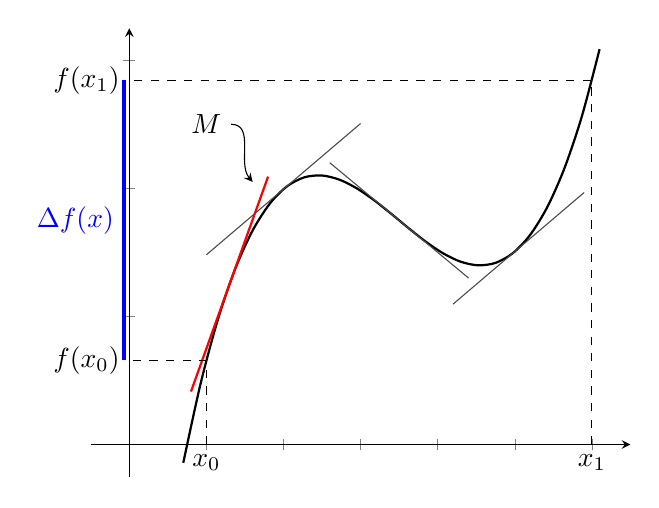
\begin{tikzpicture}[
				declare function = {
					curve(\x) = 0.3*(\x-3.5)^3-\x+7;
					derivative(\x) = (9*(\x-7/2)^2)/10-1;
					x_0=1;
					x_1=6;
				},
				> = stealth]
				\begin{axis}[
					axis lines = center,
					%axis equal,
					%ymax = 3, ymin = -1,
					xmin = -.5, xmax= 6.5,
					ymin = -.5, ymax= 6.5,
					xticklabels={,,}, yticklabels={,,},
					clip mode = individual
				]
					\addplot[domain=.7:6.1, smooth, thick] {curve(x)};
					% Tangents
					\addplot[domain=.8:1.8, color=red, thick] {(x-1.3)*derivative(1.3) + curve(1.3)};
					\addplot[domain=1:3, color=black!70] {(x-2)*derivative(2) + curve(2)};
					\addplot[domain=2.6:4.4, color=black!70] {(x-3.5)*derivative(3.5) + curve(3.5)};
					\addplot[domain=4.2:5.9, color=black!70] {(x-5)*derivative(5) + curve(5)};
					% Dashed lines
					\pgfplotsinvokeforeach{x_0,x_1} {
						\draw[dashed] (#1, 0) node[below]{$#1$} |- (0,{curve(#1)}) node[left] {$f(#1)$};
					}
					% Notes
					\node (M) [align=center] at (1, 5) {$M$};
					\draw[thin, ->] (M.east) to [out=0, in=130](1.6, 4.1);
					\node[align=center, color=blue] at (-.7, 3.5) {$\Delta f(x)$};
					\draw[ultra thick, color=blue] (-.07, {curve(x_0)}) -- (-.07, {curve(x_1)});
				\end{axis}
			\end{tikzpicture}
		\end{center}
		Si può notare che, preso l'$M$ identificato graficamente, si ha $\abs{f(x_1) - f(x_0)} \leq M \cdot \abs{x_1 - x_0}$ come da enunciato.
	\end{note}
	\begin{proof}
		Si può dare per scontato che $x_1 \neq x_0$, in quanto, se $x_1 = x_0$ , allora $f(x_1) = f(x_0)$ e la \cref{eq:accresc_fin} diventerebbe $0 \leq 0$. La tesi sarebbe quindi verificata direttamente.\\
		Fissato un qualsiasi $v \in \R^m$, si definisce così la funzione $F$ legata ad $f$ tramite la \fullref{def:segmento}:
		\begin{equation}
			\label{eq:accresc_fin_F}
			\funcdef{F}{\intervalclose{0}{1}}{\R}{t}{v \cdot f \bigl( t x_1 + (1-t)x_0 \bigr)}
		\end{equation}
		\begin{note}
			Nella \cref{eq:accresc_fin_F},  $\cdot$  è Prodotto Scalare tra due vettori di dimensione $\R^m$, dunque il risultato è correttamente uno scalare.
		\end{note}
		$F$ è continua e derivabile sull'intervallo di definizione $\intervalclose{0}{1}$. È dunque possibile utilizzare il \fullref{teo:lagrange}, che garantisce:
		\[\exists c \in \intervalopen{0}{1}: \quad F(1) - F(0) = F'(c) \; (1-0)\]
		Tornando dunque a $f$ dalla definizione di $F$
		\[v \cdot f(x_1) - v \cdot f(x_0) = v \cdot Df\bigl( cx_1 + (1-c)x_0 \bigr) (x_1 - x_0)\]
		Ricordando che la $F$ è a valori in $\R$, si può calcolare il valore assoluto mantenendo l'uguaglianza
		\[\abs{v \cdot f(x_1) - v \cdot f(x_0)} = \abs{v \cdot Df\bigl( cx_1 + (1-c)x_0 \bigr) (x_1 - x_0)}\]
		Essendo il secondo membro il valore assoluto di un prodotto scalare, si può applicare ad esso la \reffull{ex:disug_cau_schwa_matr} ed ottenere: \index{Disuguaglianza!Cauchy-Schwarz}
		\[\abs{v \cdot \bigl( f(x_1) - f(x_0) \bigr)} \leq \norm{v} \cdot \norm{Df\bigl( cx_1 + (1-c)x_0 \bigr) (x_1 - x_0)}\]
		Dunque, separando ulteriormente le norme si arriva alla:
		\begin{equation}
			\label{eq:accr_fin_norm}
			\abs{v \cdot \bigl( f(x_1) - f(x_0) \bigr)} \leq \norm{v} \cdot \norm{Df\bigl( cx_1 + (1-c)x_0 \bigr)} \cdot \norm{x_1 - x_0}
		\end{equation}
		Essendo, come detto all'inizio, $f(x_1) \neq f(x_0)$ è ora possibile scegliere un $v$ "comodo", come:
		\[v = \frac{1}{\norm{f(x_1) - f(x_0)}} \cdot \bigl( f(x_1) - f(x_0) \bigr)\]
		\begin{note}
			La norma di $v$, grazie poi alla proprietà \ref{itm:def_norm_propr_lambda} da \fullref{def:norma}, è
			\begin{align*}
				\norm{v} &= \norm{
					\underbrace{\frac{1}{\norm{f(x_1) - f(x_0)}}}_{\text{Scalare}}
					\cdot
					\underbrace{\bigl( f(x_1) - f(x_0) \bigr)}_{\text{Vettore}}
					}\\
				&= \abs{\frac{1}{\norm{f(x_1) - f(x_0)}}} \cdot \norm{\bigl( f(x_1) - f(x_0) \bigr)}\\
				&= \frac{1}{\norm{f(x_1) - f(x_0)}} \cdot \norm{\bigl( f(x_1) - f(x_0) \bigr)}\\
				&= 1
			\end{align*}
		\end{note}
		Sostituendo dunque in \cref{eq:accr_fin_norm} si ottiene
		\[\norm{\frac{1}{\norm{f(x_1) - f(x_0)}} \cdot \bigl( f(x_1) - f(x_0) \bigr) \cdot \bigl( f(x_1) - f(x_0) \bigr)} \leq \cdot \norm{Df\bigl( cx_1 + (1-c)x_0 \bigr)} \cdot \norm{x_1 - x_0}\]
		Dalla \hyperlink{note:ex_sp_norm_Rn}{\notestyle{} al punto \ref*{itm:ex_sp_norm_Rn} di \fullref*{ex:sp_norm}}, si ottiene
		\[\norm{\frac{1}{\norm{f(x_1) - f(x_0)}} \cdot \norm{f(x_1) - f(x_0)}^2} \leq \norm{Df\bigl( cx_1 + (1-c)x_0 \bigr)} \cdot \norm{x_1 - x_0}\]
		Da cui
		\[\norm{f(x_1) - f(x_0)} \leq \norm{Df\bigl( cx_1 + (1-c)x_0 \bigr)} \cdot \norm{x_1 - x_0}\]
		e passando al $\sup$ su $t \in \intervalopen{0}{1}$ si ottiene la tesi.
	\end{proof}
\end{theorem}
Il seguente esercizio mostra come il \fullref{teo:lagrange} non possa essere esteso al caso di funzioni a valori in $\R^n$ con $n > 1$.
\begin{exercise}
	Sia $f: \R \to \R^2$ data da $f(t) = (\cos t, \sin t)$. Mostrare che non esiste nessun numero reale $c$ tale che
	\[f(2 \pi) - f(0) = Df(c) \cdot 2 \pi\]
\end{exercise}

\begin{definition}[Insieme Convesso]
	\index{Insieme!Convesso}
	\label{def:convesso}
	Sia $C \subseteq \R^n$
	\begin{equation*}
		\begin{gathered}
			C \text{ è \textbf{Convesso}}\\
			\bydef\\
			\forall x_0,y_1 \in C \quad \brackets{tx_1+(1-t)x_0:\; t \in \intervalclose{0}{1}} \subseteq C
		\end{gathered}
	\end{equation*}
	Cioè un insieme è Convesso se, dati qualsiasi due suoi punti, contiene anche il segmento che li congiunge.
\end{definition}
\begin{exercise}
	Dimostrare la \fullref{prop:convesso_deriv_par_lim_allora_lips}
	% TODO solution
\end{exercise}
\begin{exercise}
	In $\R^n$ dimostrare che ogni segmento è convesso, così come anche ogni sfera.\\
	Esibire un esempio di insieme non convesso.
	% TODO solution
\end{exercise}
\begin{corollary}
	\label{coro:convess_nabla_0_f_const}
	Siano $A \subseteq \R^n$ e $f: A \to \R$
	\[
		\left.
			\begin{array}{c}
				A \text{ \textbf{Aperto Convesso}}\\[-1ex]
				e\\[-0.5ex]
				f \text{ \textbf{Differenziabile} in } A\\[-1ex]
				e\\[-0.5ex]
				\forall x \in A \quad \nabla f(x) = 0
			\end{array}
		\right\}
		\quad \implies \quad
		f \text{ è \textbf{Costante} su } A
	\]
	\vspace*{-\baselineskip}
	\begin{note}
		Come da \fullref{obs:matr_deriv_tot}, $\nabla f(x) = Df(x) \in \mat (1 \times n)$, cioè un vettore riga.
	\end{note}
	\begin{proof}
		Se $\nabla f(x) = Df(x) = 0$, la \cref{eq:accresc_fin} da \fullref{teo:accresc_fin} diventa
		\begin{equation*}
			\begin{gathered}
				\norm{f(x_1) - f(x_0)} \leq \sup\limits_{\xi \in S} 0 \cdot \norm{x_1-x_0}\\
				\norm{f(x_1) - f(x_0)} \leq 0\\
				f(x_1) = f(x_0)
			\end{gathered}
		\end{equation*}
	\end{proof}
\end{corollary}
\begin{exercise}
	Dimostrare che un insieme \textbf{Convesso} è anche \textbf{Connesso}.\\
	Esibire un controesempio al viceversa.
	\begin{solution}
		Supponendo, per assurdo, $C \in \R^n$ sconnesso. In questo caso, per \fullref{def:connesso}, esistono due insiemi separati $S_1$ e $S_2$ che costituiscono $C$, inoltre $S_1 \cup S_2 = C$ e $S_1 \cap S_2 = \emptyset$. Questo implica che
		\[\exists t \in \intervalclose{0}{1}:\; \forall x_1 \in S_1 \text{ e } \forall x_2 \in S_2 \quad tx_1 + (1-t)x_2 \notin S_1 \text{ e contemporaneamente } \notin S_2\]
		Questo implica la non convessità di $C$ - \textit{Assurdo}.
	\end{solution}
	\begin{solution}
		Preso il cerchio di raggio unitario $S = {(x,y): x^2 + y^2 = 1}$, questo verifica la \fullref{def:connesso} ma sicuramente non la \fullref{def:convesso}.
	\end{solution}
\end{exercise}
\begin{exercise}
	Esibire esempi di insiemi convessi/non convessi e aperti/chiusi, limitati/illimitati.
	% TODO solution
\end{exercise}

\begin{definition}[Funzione Convessa]
	\index{Funzione!Convessa}
	Sia $I$ un intervallo reale e $f:\; I \to \R$.
	\begin{equation*}
		f \text{ è \textbf{Convessa}}
		\quad \bydef \quad
		\begin{cases}
			\forall x_0, x_1 \in I,\; \forall t \in \intervalclose{0}{1}\\
			f \bigl( (1-t)x_0 + t x_1 \bigr) \leq (1-t) f(x_0) + t f(x_1)
		\end{cases}
	\end{equation*}
	Cioè se il segmento che congiunge due qualsiasi punti del suo grafico si trova al di sopra del grafico stesso.
\end{definition}
\begin{exercise}
	\index{Epigrafo}
	Verificare che $f$ è \textbf{Convessa} se e solo se il suo \textbf{Epigrafo} (cioè l'insieme di punti che stanno al di sopra o sul grafico della funzione)
	è un sottoinsieme \textbf{Convesso} di $\R^2$ nel senso della \fullref{def:convesso}.
	% TODO solution
\end{exercise}
\begin{proposition}
	Siano $A \subseteq \R^n$ e $f: A \to \R$
	\[
		\left.
			\begin{array}{c}
				A \text{ \textbf{Aperto Connesso}}\\[-1ex]
				e\\[-0.5ex]
				f \text{ \textbf{Differenziabile} in } A\\[-1ex]
				e\\[-0.5ex]
				\forall x \in A \quad \nabla f(x) = 0
			\end{array}
		\right\}
		\quad \implies \quad
		f \text{ è \textbf{Costante} su } A
	\]
	\vspace*{-\baselineskip}
	\begin{note}
		Si sta parlando di insiemi \textbf{Connessi}
	\end{note}
	\begin{proof}
		Sia $x_0 \in A$. Per la \fullref{prop:polig_in_aperto_connesso}, ogni punto $x \in A$ può essere unito a $x_0$ con una poligonale interamente contenuta in $A$ dai lati paralleli agli assi. A questo punto è possibile applicare il \fullref{teo:accresc_fin} ad ogni segmento della poligonale ed, essendo $\nabla f(x) = 0$, come in \fullref{coro:convess_nabla_0_f_const}, la $f$ è costante.
	\end{proof}
\end{proposition}

\newpage
\section{Derivate Seconde}
Quanto detto circa le derivate prime può essere ripetuto introducendo derivate di ordine superiore.
\begin{definition}[Derivate Parziali Seconde]
	\index{Derivata!Parziali Seconde}
	Sia $f: A \to \R^m$ con $A \subseteq \R^n$ derivabile parzialmente in $x_0$ lungo $e_i$.\\
	Se la funzione $\frac{\partial f}{\partial x_i}$ è a sua volta derivabile parzialmente in $x_0$, questa volta lungo $e_j$, allora la quantità
	\[
		\frac{\partial}{\partial x_j} \frac{\partial f}{\partial x_i} (x_0)
		\quad \bydef \quad
		\begin{array}{c}
			\text{ è la \textbf{Derivata Parziale Seconda}}\\
			\text{di } f \text{ in } x_0 \text{ rispetto a } x_j, x_i \text{ (in quest'ordine)}
		\end{array}
	\]
	e si indica con
	\[\boldsymbol{\frac{\partial^2 f}{\partial x_j \partial x_i} (x_0)}\]
	\vspace*{-\baselineskip}
	\begin{note}
		Altre notazioni comunemente utilizzate sono: $D^2_{x_j x_i} f ,\;\; \partial^2_{ji} f ,\;\; \partial_{x_j x_i} f ,\;\; f_{x_j x_i} ,\;\; f_{ji}$
	\end{note}
	\begin{note}
		L'ordine qui utilizzato, cioè
		\[\frac{\partial^2 f}{\partial x_j \partial x_i} = \frac{\partial}{\partial x_j} \frac{\partial f}{\partial x_i} \qquad i,j = 1,\:\dotsc\:,n\]
		non è sempre condiviso da tutti i testi di Analisi Matematica.
	\end{note}
\end{definition}
\begin{observation}
	Le regole di derivazione fornite in \fullref{sect:regole_deriv} sono adeguate anche per il calcolo delle Derivate Seconde.
\end{observation}
\begin{exercise}
	\label{ex:num_deriv_sec}
	Siano $A \subseteq \R^n$ e $f:A \to \R^m$. Ammesso che esistano tutte, quante sono le derivate parziali seconde di $f$ in un qualche punto $x_0$?\\
	Confrontare quanto ottenuto con il caso $n = m = 1$ di Analisi 1.
	\begin{solution}
		Ognuna delle $n$ derivate di $f$ ha, a sua volta, $n$ derivate, di conseguenza il numero di derivate seconde di $f$ è $n^2$. Nel caso di Analisi 1, le derivate seconde erano $1^2 = 1$
	\end{solution}
\end{exercise}

\begin{definition}[Differenziale Secondo]
	\index{Differenziale!Secondo}
	\label{def:differenz_second}
	Siano $A \subseteq \R^n$, $f:A \to \R^m$ e $x_0 \in \circdot{A}$
	\[
		f \text{ è \textbf{Differenziabile} } 2 \text{ volte in } x_0
		\quad \bydef \quad
		\begin{cases}
			\begin{array}{c}
				f \text{ è \textbf{Differenziabile} in un intorno di } x_0\\
				e\\
				f' \text{ è \textbf{Differenziabile} in } x_0
			\end{array}
		\end{cases}
	\]
	Dove $f'$ è una funzione definita in un intorno di $x_0$ a valori in $\mat(m \times n) \in \R^{mn}$.
	\begin{note}
		Questa definizione è utilizzata comunemente nel linguaggio parlato, ma viene raramente formalizzata come definizione.
	\end{note}
	\begin{note}
		Avendo una funzione	\textit{scalare} $f: A \to \R$ con $A \subseteq \boldsymbol{\R^n}$, la sua derivata prima è un \textit{vettore}. La derivata seconda sarà una \textit{matrice} e così via.
	\end{note}
\end{definition}

\begin{definition}[Matrice Hessiana]
	\index{Matrice!Hessiana}
	\label{def:hessiana}
	Siano $A \subseteq \R^n$, $f:A \to \R^m$ e $x_0 \in \circdot{A}$, inoltre $f$ ammette tutte le Derivate Parziali Seconde in $x_0$.\\
	La matrice di queste derivate seconde si chiama \textbf{Matrice Hessiana} di $f$ in $x_0$ e si indica con $\boldsymbol{H_f(x_0)}$
	\[
		H_f(x_0) = D^2f(x_0) =
		\begin{bmatrix}
			\dfrac{\partial^2 f}{\partial x_1 \partial x_1} & \dfrac{\partial^2 f}{\partial x_2 \partial x_1} & \dots & \dfrac{\partial^2 f}{\partial x_n \partial x_1}\\[3ex]
			\dfrac{\partial^2 f}{\partial x_1 \partial x_2} & \dfrac{\partial^2 f}{\partial x_2 \partial x_2} & \dots & \dfrac{\partial^2 f}{\partial x_n \partial x_2}\\[3ex]
			\vdots & \vdots & \ddots & \vdots\\[3ex]
			\dfrac{\partial^2 f}{\partial x_1 \partial x_n} & \dfrac{\partial^2 f}{\partial x_2 \partial x_n} & \dots & \dfrac{\partial^2 f}{\partial x_n \partial x_n}
		\end{bmatrix}
	\]
	\begin{note}
		La Matrice Hessiana non va confusa con la Matrice Jacobiana da \fullref{obs:matr_deriv_tot}, quest'ultima infatti è la matrice delle Derivate Parziali \textbf{Prime}, mentre la Hessiana contiene le \textbf{Seconde}.
	\end{note}
\end{definition}

\subsection{Il Lemma di Schwarz}
\begin{lemma}[di Schwarz]
	\index{Lemma!di Schwarz}
	\label{lemma:schwarz}
	Siano $A \subseteq \R^2$, $f:A \to \R^m$ e $(x_0, y_0) \in \circdot{A}$. Se $\frac{\partial^2 f}{\partial x \partial y}$ e $\frac{\partial^2 f}{\partial y \partial x}$ \textbf{esistono} in un intorno di $(x_0, y_0)$ e sono \textbf{Continue} in $(x_0, y_0)$, allora
	\[\frac{\partial^2 f}{\partial x \partial y} \quad = \quad \frac{\partial^2 f}{\partial y \partial x}\]
	\begin{proof}
		Scelti $h, k \in \R$ sufficientemente piccoli, in modo tale che le derivate parziali di $f$ siano definite in tutto il rettangolo di estremi
		\[(x_0, y_0) \qquad\qquad (x_0 + h, y_0) \qquad\qquad (x_0, y_0 + k) \qquad\qquad (x_0 + h, y_0 + k)\]
		\begin{center}
			\begin{tikzpicture}
				\pgfmathsetmacro\MAX{8}
				\pgfmathsetmacro\XZ{\MAX / 3 }
				\pgfmathsetmacro\YZ{\MAX / 3 }
				\pgfmathsetmacro\XZh{\MAX / 3 *2}
				\pgfmathsetmacro\YZk{\MAX / 3 *2}
				\coordinate (X0Y0) at (\XZ,\YZ);
				\coordinate (X0hY0) at (\XZh,\YZ);
				\coordinate (X0Y0k) at (\XZ,\YZk);
				\coordinate (X0hY0k) at (\XZh,\YZk);

				\draw[->] (0,0) -- (\MAX,0) node[anchor=north west] {$x$};
				\draw[->] (0,0) -- (0,\MAX) node[anchor=south east] {$y$};
				\draw[dotted] (\XZ,0) -- (\XZ,\MAX);
				\draw[dotted] (0,\YZ) -- (\MAX,\YZ);
				\draw[dotted] (\XZh,0) -- (\XZh,\MAX);
				\draw[dotted] (0,\YZk) -- (\MAX,\YZk);
				\draw node[anchor=north] at (\XZ,0) {$x_0$};
				\draw node[anchor=north] at (\XZh,0) {$x_0+h$};
				\draw node[anchor=east] at (0,\YZ) {$y_0$};
				\draw node[anchor=east] at (0,\YZk) {$y_0+k$};
				\draw node at (X0Y0) {$\bullet$};
				\draw node at (X0Y0k) {$\bullet$};
				\draw node at (X0hY0) {$\bullet$};
				\draw node at (X0hY0k) {$\bullet$};
			\end{tikzpicture}
		\end{center}
		Per come son state scelte $h$ e $k$, è possibile definire sicuramente la quantità
		\[q = f(x_0 + h, y_0 + k) - f(x_0 + h, y_0) - f(x_0, y_0 + k) + f(x_0, y_0)\]
		Per dimostrare la tesi si può ora verificare che la $q$, calcolata lungo percorsi differenti fornisce lo stesso risultato. È possibile fare ciò riconducendo la $q$ a due diverse funzioni in una sola variabile ed applicando il \fullref{teo:lagrange} due volte ad ognuna di esse.
		\begin{enumerate}
			\item Posta $\varphi(\xi) = f(x_0 + \xi, y_0 + k) - f(x_0 + \xi, y_0)$, si ottiene, riordinando i termini della $q$
				\begin{align*}
					q &= \Bigl( f(x_0 + h, y_0 + k) - f(x_0 + h, y_0) \Bigr) - \Bigl( f(x_0, y_0 + k) - f(x_0, y_0) \Bigr)\\
					&= \varphi(h) - \varphi(0)
					\shortintertext{Applicando Lagrange}
					&= h\: \varphi'(\alpha' h)
					\shortintertext{Grazie alla \fullref{prop:diff_somma_funz} si passa alle derivate parziali rispetto a $x$ (la $y$ è fissa)}
					&= h \left( \frac{\partial f}{\partial x}(x_0 + \alpha' h, y_0 + k) - \frac{\partial f}{\partial x}(x_0 + \alpha' h, y_0) \right)
					\intertext{Si definisce ora $\Phi(\xi) = \frac{\partial f}{\partial x}(x_0 + \alpha'h, y_0 + \xi)$}
					&= h \bigl( \Phi(k) - \Phi(0) \bigr)
					\shortintertext{Per la $\Phi$ valgono nuovamente le ipotesi di Lagrange, dunque si ottiene}
					&= hk\: \Phi'(\beta' k)\\
					&= hk\: \frac{\partial^2 f}{\partial y \partial x}(x_0 + \alpha' h, y_0 + \beta' k)
				\end{align*}
			\item Posta $\psi(\xi) = f(x_0 + h, y_0 + \xi) - f(x_0, y_0 + \xi)$, si ottiene, riordinando i termini della $q$
				\begin{align*}
					q &= \Bigl( f(x_0 + h, y_0 + k) - f(x_0, y_0 + k) \Bigr) - \Bigl( f(x_0 + h, y_0) - f(x_0, y_0) \Bigr)\\
					&= \psi(k) - \psi(0)
					\shortintertext{Applicando Lagrange}
					&= k\: \psi'(\beta'' k)
					\shortintertext{Grazie alla \fullref{prop:diff_somma_funz} si passa alle derivate parziali rispetto a $y$ (la $x$ è fissa)}
					&= k \left( \frac{\partial f}{\partial y}(x_0 + h, y_0 + \beta'' k) - \frac{\partial f}{\partial y}(x_0, y_0 + \beta'' k) \right)
					\intertext{Si definisce ora $\Psi(\xi) = \frac{\partial f}{\partial y}(x_0 + \xi, y_0 + \beta'' k)$}
					&= k \bigl( \Psi(h) - \Psi(0) \bigr)
					\shortintertext{Per la $\Psi$ valgono nuovamente le ipotesi di Lagrange, dunque derivando rispetto a $x$ si ottiene}
					&= kh\: \Psi'(\alpha'' h)\\
					&= kh\: \frac{\partial^2 f}{\partial x \partial y}(x_0 + \alpha'' h, y_0 + \beta'' k)
				\end{align*}
		\end{enumerate}
		Si è quindi giunti a due diverse formulazioni di $q$ per degli $\alpha', \alpha'', \beta', \beta'' \in \intervalopen{0}{1}$
		\[\cancel{hk}\: \frac{\partial^2 f}{\partial y \partial x}(x_0 + \alpha' h, y_0 + \beta' k) = \cancel{kh}\: \frac{\partial^2 f}{\partial x \partial y}(x_0 + \alpha'' h, y_0 + \beta'' k)\]
		A questo punto si calcola il limite per $(h, k) \to (0, 0)$. Spostandosi, anche $\alpha', \alpha'', \beta', \beta''$ cambieranno, ma essendo limitati $\in \intervalopen{0}{1}$, non si presentano complicazioni di sorta in quanto vengono moltiplicati per una quantità tendente a zero.
		\[\frac{\partial^2 f}{\partial y \partial x}(x_0, y_0) = \frac{\partial^2 f}{\partial x \partial y}(x_0, y_0)\]
	\end{proof}
\end{lemma}
\begin{observation}
	Il \fullref{lemma:schwarz} ha importanti applicazioni in fisica e nella teoria dei campi. Grazie al lemma è infatti possibile distinguere tra campi \textbf{conservativi} e non: uno dei criteri è appunto il controllo dell'uguaglianza dell derivate parziali miste.
\end{observation}
\begin{exercise}
	Verificare se il \fullref{lemma:schwarz} si applica alla funzione
	\[\funcdef{f}{\R^2}{\R}{(x,y)}{
		\begin{cases}
			\begin{array}{ll}
				\dfrac{x^3 y - xy^3}{x^2 + y^2} & \text{se } (x,y) \neq (0,0)\\
				0 & \text{se } (x,y) = (0,0)
			\end{array}
		\end{cases}
	}\]
\end{exercise}
\begin{corollary}
	Siano $A \subseteq \R^n$, $f:A \to \R^m$ e $x_0 \in \circdot{A}$. Se $\frac{\partial^2 f}{\partial x_i \partial x_j}$ e $\frac{\partial^2 f}{\partial x_j \partial x_i}$ \textbf{esistono} in un intorno di $x_0$ e sono \textbf{Continue} in $x_0$, allora
	\[\frac{\partial^2 f}{\partial x_i \partial x_j} \quad = \quad \frac{\partial^2 f}{\partial x_j \partial x_i}\]
	\begin{proof}
		Segue dal \fullref{lemma:schwarz} applicandolo a tutte le variabili prese 2 a 2.
	\end{proof}
\end{corollary}

\begin{definition}[Funzioni di Classe $\cntclass{2}$]
	\index{Classe!$\cntclass{2}$}
	Sia $A \subseteq \R^n$ un \textbf{Aperto}.
	\begin{center}
		$\cntclass{1}(A; \R^m)$ è l'insieme delle funzioni $f:A \to \R^m$\\
		con \textbf{tutte} le \textbf{Derivate Parziali seconde continue} in ogni punto di $A$
	\end{center}
	Si può anche leggere \textit{$f$ è di classe $\cntclass{2}$ su $A$ con valori in $\R^m$}.
\end{definition}

\begin{corollary}
	Sia $A \subseteq \R^n$ un aperto.
	\[f \in \cntclass{2}(A;\R) \quad \implies \quad D^2 f \text{ è una matrice \textbf{simmetrica}}\]
	\begin{proof}
		Segue dal \fullref{lemma:schwarz}, in quanto $\frac{\partial^2 f}{\partial x_i \partial x_j} = \frac{\partial^2 f}{\partial x_j \partial x_i}$ per ogni $i, j$ della matrice, andando a verificare la definizione di Matrice Simmetrica.
	\end{proof}
\end{corollary}
\begin{exercise}
	Siano $A \subseteq \R^n$ e $f \in \cntclass{2}(A;\R^m)$.\\
	Quante sono le derivate parziali seconde di $f$ che bisogna necessariamente calcolare? Calcolare questa risposta con quella dell'\fullref{ex:num_deriv_sec}.
	\begin{solution}
		Bisogna calcolare $\frac{n(n+1)}{2}$ derivate diverse, invece che $n^2$.
	\end{solution}
\end{exercise}
\begin{exercise}
	Esibire un esempio di funzione $f:\R^2 \to \R$ che ammetta tutte le derivate parziali seconde in un punto, ma che non sia continua in quel punto
	% TODO solution
\end{exercise}

\subsection{Sviluppo in Serie di Taylor al II Ordine}
Fino ad ora son stati visti 2 "livelli" di approssimazione di una funzione $f$ in un intorno del punto $x_0$, appartenente all'insieme di definizione di $f$. Per $x \to x_0$:
\begin{itemize}
	\item Livello $0$: \quad $f$ continua \qquad $f(x) = f(x_0) + o(1)$
	\item Livello $1$: \quad $f$ derivabile \qquad $f(x) = f(x_0) + f'(x_0)(x - x_0) + o(x - x_0)$
\end{itemize}
A livello $0$, la funzione è stata approssimata dal \textit{miglior} polinomio di grado $0$, cioè la costante $f(x_0)$; a livello $1$ dal \textit{miglior} polinomio di grado $1$, $f(x) = f(x_0) + f'(x_0)(x - x_0)$. Per \textit{migliore} si intende che usando un qualsiasi altro polinomio di grado $1$ passante per $\bigl( x_0, f(x_0) \bigr)$ il resto sarebbe andato a $0$ come $x - x_0$ e non più velocemente. Queste approssimazioni ci permettono di capire se una funzione sia crescente o meno, ma non è possibile, ad esempio, studiarne la concavità. Per ottenere più informazioni è possibile estendere questi risultati a polinomi di grado superiore al primo.\\
Come nel caso Analisi 1, gli \textbf{Sviluppi di Taylor} permettono di approssimare localmente una funzione con un polinomio nelle variabili indipendenti a patto di conoscere opportune derivate parziali della funzione.

\vspace*{\baselineskip}
\cbstart
La seguente sezione affiancata da una banda verde non è richiesta, in quanto non presente nel testo di riferimento. È però necessaria per chiarire i concetti con cui si sta lavorando, deve quindi essere considerata come un approfondimento da leggere.
\begin{definition}[Polinomio di Taylor]
	\index{Polinomio di Taylor}
	\label{def:pol_taylor}
	Siano:
	\begin{itemize}[noitemsep]
		\item $f \in \cntclass{n}(A;\R^m)$ con $A \subseteq \R^n$
		\item $x_0 \in \circdot{A}$
		\item $h \in \R^n \setminus \brackets{0}$
		\item Il segmento di estremi $x_0$ e $x_0 + h$ è interamente contenuto in $A$
	\end{itemize}
	Allora
	\[T_{n-1}(f, x_0) = f(x_0) + Df(x_0; h) + \frac{1}{2!} D^2f(x_0; h) + \cdots + \frac{1}{(n-1)!} D^{n-1}f(x_0; h)\]
	Oppure, in forma più compatta
	\begin{equation}
		\label{eq:pol_taylor}
			T_{n-1}(f, x_0) = \sum\limits_{i = 1}^{n-1} \frac{1}{i!} D^if(x_0; h)
	\end{equation}
	si dice \textbf{Polinomio di Taylor} di grado $n-1$ della funzione $f$ centrato nel punto $x_0$.

	\begin{samepage}
		\begin{note}
			Nella \cref{eq:pol_taylor}, con la forma $D^if(x_0; h)$ si intende lo \textit{scalare} ottenuto applicando all’incremento $h$ il differenziale $i$\textit{-esimo} calcolato in $x_0$.\\
			Supponendo $f: \R^n \to \R^1$, la $D^if(x_0; h)$ diventa, ad esempio:
			\begin{itemize}
				\item $i = 1 \qquad Df(x_0; h) = \nabla f(x_0) \cdot h$
				\item $i = 2 \qquad D^2f(x_0; h) = h^T \cdot H_f(x_0) \cdot h$ \quad dove $h^T$ è $h$ trasposto e $H_f$ è la \fullref{def:hessiana}
			\end{itemize}
			Con $\; \cdot \;$, in questo caso, si intende il prodotto righe per colonne.\\
			Vedasi \fullref{obs:matr_deriv_tot} per le possibile "forme" assunte dalla $Df(x_0; h)$ in base ai valori di $n$ e $m$.
		\end{note}
	\end{samepage}
\end{definition}
% \begin{observation}
% 	Il Polinomio di Taylor è caratterizzato dall'avere in comune con la funzione $f$ il valore di tutte le derivate fino all’ordine $n-1$ nel punto $x_0$.
% \end{observation}
\begin{theorem}[di Taylor]
	\index{Teorema!di Taylor}
	\label{teo:taylor}
	Siano:
	\begin{itemize}[noitemsep]
		\item $f \in \cntclass{n}(A;\R^m)$ con $A \subseteq \R^n$
		\item $x_0 \in \circdot{A}$
		\item $h \in \R^n \setminus \brackets{0}$
		\item Il segmento di estremi $x_0$ e $x_0 + h$ è interamente contenuto in $\circdot{A}$
	\end{itemize}
	Allora, posto $x = x_0 + h$
	\[f(x) = T_{n-1}(f, x_0) + R_n(f, x_0, h) \qquad \text{per } x \to x_0 \text{ (cioè } h \to 0\text{)}\]
	Dove $R_n(f, x_0, h)$ è \textbf{Resto} espresso nella forma di Peano o di Lagrange.
	\begin{proof}
		Omessa.
	\end{proof}
\end{theorem}

\begin{definition}[Resto di Peano]
	\index{Resto!di Peano}
	\label{def:resto_peano}
	Nelle ipotesi del \fullref{teo:taylor}, dalla \fullref{def:o_piccolo} si definisce il \textbf{resto} nella forma \textbf{di Peano}:
	\[R_n(f, x_0, h) = \frac{1}{n!} D^nf(x_0; h) + o\left( \norm{h}^2 \right)\]
	Cioè che la differenza tra la funzione ed il polinomio tende a zero quando la $x$ tende ad $x_0$, centro dello sviluppo.
\end{definition}

\begin{definition}[Resto di Lagrange]
	\index{Resto!di Lagrange}
	Nelle ipotesi del \fullref{teo:taylor}, ma con $f \in \cntclass{n}(A;\R^{\boldsymbol{1}})$ si definisce il \textbf{resto} nella forma \textbf{di Lagrange}
	\[\exists \theta \in \intervalclose{0}{1}: \quad R_n(f, x_0, h) = \frac{1}{n!} D^nf(x_0; \theta h) = \frac{D^n f(x + \theta h)}{n!} (x + \theta h)\]
	Cioè che esiste un punto (senza sapere quale sia) all'interno del segmento di estremi $x_0$ e $x_0 + h$ in cui si ha un'equivalenza precisa tra la funzione ed il polinomio.
\end{definition}
\begin{observation}
	\label{obs:resto_lagr_Rn}
	Il Resto di Lagrange, a differenza del \fullref{def:resto_peano}, offre informazioni quantitative sul resto, ma \textbf{NON} è applicabile a funzioni a valori in $\R^m$, solo a funzioni a valori reali.
\end{observation}
\cbend

\noindent Si passa ora al caso specifico degli sviluppi del secondo ordine

\begin{samepage}
	\begin{proposition}[Sviluppo di Taylor al Secondo Ordine con resto di Peano]
		\index{Sviluppo di Taylor!con Resto di Peano}
		\label{prop:svil_tay_2_peano}
		Siano:
		\begin{itemize}[noitemsep]
			\item $f \in \cntclass{2}(A;\R^m)$ con $A \subseteq \R^n$
			\item $x_0 \in \circdot{A}$
			\item $h \in \R^n \setminus \brackets{0}$
			\item Il segmento di estremi $x_0$ e $x = x_0 + h$ è interamente contenuto in $\circdot{A}$
		\end{itemize}
		Allora, posto $x = x_0 + h$
		\[
			f(x) = f(x_0) + Df(x_0)h + \frac{1}{2} h^T D^2f(x_0) h + o\left( \norm{h}^2 \right)
			\qquad
			\text{per } x \to x_0 \text{ (cioè } h \to 0\text{)}
		\]
		\begin{note}
			$h^T$ è il vettore riga trasposto del vettore colonna $h$.
		\end{note}
		Alternativamente, la formula precedente si può anche esprimere in questo modo, con $t \in \R$ e $x = x_0 + th$
		\[
			f(x) = f(x_0) + t Df(x_0) h + \frac{1}{2} t^2 h^T D^2f(x_0) h + o\left( t^2 \right)
			\qquad \text{per } t \to 0
		\]
		\begin{proof}
			Omessa in aula.

			\cbstart
			Eseguire lo sviluppo di Taylor centrato in $t = 0$ della funzione di variabile reale $\varphi(t) = f(x_0 + th)$ con Resto di Peano.
			\cbend
		\end{proof}
	\end{proposition}
\end{samepage}

\begin{proposition}[Sviluppo di Taylor al Secondo Ordine con resto di Lagrange]
	\index{Sviluppo di Taylor!con Resto di Lagrange}
	Siano:
	\begin{itemize}[noitemsep]
		\item $f \in \cntclass{2}(A;\R)$ con $A \subseteq \R^n$
		\item $x_0 \in \circdot{A}$
		\item $h \in \R^n \setminus \brackets{0}$
		\item Il segmento di estremi $x_0$ e $x_0 + h$ è interamente contenuto in $\circdot{A}$
	\end{itemize}
	Allora, posto $x = x_0 + h$, esiste un $\theta \in \intervalclose{0}{1}$ tale che
	\[f(x) = f(x_0) + Df(x_0)h + \frac{1}{2} h^T D^2 f(x_0 + \theta h) h\]
	\begin{note}
		Come detto in \fullref{obs:resto_lagr_Rn}, il Resto di Lagrange dà un risultato esatto, ma si può applicare solo a funzioni in $\R$.
	\end{note}
	\begin{proof}
		Omessa in aula.

		\cbstart
		Eseguire lo sviluppo di Taylor centrato in $\theta = 0$ della funzione di variabile reale $\varphi(\theta) = f(x_0 + \theta h)$ con Resto di Lagrange.
		\cbend
	\end{proof}
\end{proposition}

\begin{exercise}
	Sfruttando i noti sviluppi di funzioni reali di una variabile reale, scrivere lo sviluppo di Taylor al secondo ordine centrato nell'origine delle seguenti funzioni:
	\begin{align*}
		(x,y) &\mapsto 2x^2 + 3xy + 4xy^3 &
		(x,y) &\mapsto e^{x-y^2} \ln(1+x+y^2) &
		(x,y,z) &\mapsto \sin(x + 3z) \cos(z - y) \\
		%
		(x,y) &\mapsto \sin(xy) &
		(x,y,z) &\mapsto \sqrt{1+2x+3y+4z} &
		(x,y) &\mapsto \frac{x+y^2}{\cos (x+y)} \\
		%
		(x,y,z) &\mapsto (x+z) \cos (2x+3y) &
		(x,y) &\mapsto \begin{bmatrix}
			\cos(x^2 + y^2)\\
			\sin(x^2 - y^2)
		\end{bmatrix} &
		(x,y,z) &\mapsto \begin{bmatrix}
			z \ln (1 + xy)\\
			\frac{y}{1+x+z}\\
			(y + z) \sin x
		\end{bmatrix}
	\end{align*}
\end{exercise}

\subsection{Derivate di Ordine Superiore}
\begin{definition}
	\index{Classe!$\cntclass{n}$}
	\index{Classe!$\cntclass{\infty}$}
	Sia $k \in \N$ e sia $A \subseteq \R^n$ un \textbf{Aperto}. $\cntclass{0}(A;\R^m)$ è l'insieme delle funzioni continue su $A$ con valori in $\R^m$. Se $k \geq 1$, $\cntclass{k}(A;\R^m)$ è l'insieme delle funzioni continue su $A$ con valori in $\R^m$ con tutte le derivate parziali prime di classe $\cntclass{k-1}$ su $A$.\\
	Inoltre
	\[\cntclass{\infty}(A;\R^m) = \bigcap\limits_{k \in \N}\cntclass{k}(A;\R^m)\]
	Si può anche leggere \textit{$f$ è di classe $\cntclass{k}$ o $\cntclass{\infty}$ su $A$ con valori in $\R^m$}.
\end{definition}
\begin{exercise}
	Siano $A \subseteq \R^n$ ed $f \in \cntclass{3}(A;\R^m)$. Quante sono le derivate parziali terze di $f$ in totale? E quante quelle che, in generale, bisogna necessariamente calcolare?
	% TODO solution
\end{exercise}

\newpage
\section{Il Teorema della Funzione Implicita}
I risultati esposti in questo paragrafo permettono di studiare funzioni senza averne l'espressione analitica esplicita a disposizione, fatto estremamente importante per l'utilizzo reale dell'analisi. Non è infatti sempre possibile ottenere la forma analitica di una funzione, ma ci può comunque essere necessità di studiarla.
\begin{definition}[Funzione Implicita]
	\index{Funzione!Implicita}
	\label{def:funz_impl}
	Dati
	\begin{itemize}[noitemsep]
		\item $X \subseteq \R^n, Y \subseteq \R^m$
		\item $f: X \times Y \to \R^l$
		\item $(x_0, y_0) \in X \times Y$ (un punto)
	\end{itemize}
	Si dice che l'equazione $f(x,y) = 0$ \textbf{Definisce Implicitamente una Funzione} $\varphi$ in un intorno di $(x_0,y_0)$ se:
	\begin{enumerate}
		\item $f(x_0,y_0) = 0$
		\item Esistono due aperti $\mathcal{X}$ e $\mathcal{Y}$ tali che:
			\begin{itemize}[noitemsep, topsep=0pt]
				\item $x_0 \in \mathcal{X} \subseteq X$
				\item $y_0 \in \mathcal{Y} \subseteq Y$
			\end{itemize}
			\begin{note}
				Oppure, alternativamente, $x_0 \in \circdot{\mathcal{X}}$ e $y_0 \in \circdot{\mathcal{Y}}$ con $\mathcal{X}$ e $\mathcal{Y}$ non aperti.
			\end{note}\vspace*{-2ex}
		\item Esiste $\varphi: \mathcal{X} \to \mathcal{Y}$
	\end{enumerate}
	Tali che:
	\[
		\left.
		\begin{array}{l}
			x \in \mathcal{X}\\
			y \in \mathcal{Y}\\
			f(x,y) = 0
		\end{array}
		\right\}
		\quad \implies \quad
		y = \varphi(x)
	\]
	Con $\varphi$ \textbf{Funzione Implicita} definita da $f(x,y)=0$.

	\vspace*{\baselineskip}
	Cioè la Funzione Implicita associa un sottoinsieme delle variabili dell'equazione alle variabili rimanenti. Da questo deriva il nome \textit{implicita}, in quanto la $f$ definisce "implicitamente" la $\varphi$, perché l'immagine di $f$ è influenzata da tutte le variabili della funzione, che dunque son legate tra loro.
	\begin{note}
		La \textbf{Funzione Inversa} di una qualche funzione è anche \textbf{Funzione Implicita} di questa funzione.
	\end{note}
\end{definition}
\begin{example}
	Posti $m = n = l = 1$
	\[\funcdef{f}{\R \times \R}{\R}{(x,y)}{x^2 + y^2 + 1}\]
	Non definisce alcuna funzione implicita poiché $f(x,y) = 0$ non è mai verificata.
\end{example}
\begin{example}
	Posti $m = n = l = 1$
	\[\funcdef{f}{\R \times \R}{\R}{(x,y)}{x^2 + y^2 - 1}\]
	\begin{note}
		Il Teorema della Funzione Implicita è particolarmente utile quando non è possibile esprimere in forma analitica un parametro rispetto agli altri, ma è ovviamente utilizzabile anche quando è fattibile.
	\end{note}
	Per prima cosa si osserva che è possibile trovare dei punti che verifichino l'uguaglianza $f(x,y) = 0$, cioè tutti i punti della circonferenza di raggio unitario centrata nell'origine. Il punto $(0,1)$ definisce implicitamente, tra le altre, una funzione
	\begin{equation}
		\label{eq:ese_funz_impl_cerchio}
		\funcdef{\varphi_1}{\intervalopen{-1}{1}}{\R^+}{x}{\sqrt{1-x^2}}
	\end{equation}
	\begin{note}
		$\varphi_1$ non avrebbe potuto essere definita $\intervalopen{-1}{1} \to \intervalopcl{0}{1}$ perché sarebbe contrario al punto 2 della \fullref{def:funz_impl}, non essendo $\mathcal{Y}$ un aperto, in questo caso. Estendendo $\mathcal{Y}$ a $\R^+$ si ha un aperto contenente tutti i valori assunti da $\varphi_1$.
	\end{note}
	\begin{note}
		La $\varphi_1$ di \cref{eq:ese_funz_impl_cerchio} potrebbe essere scritta in funzione di $y$ poiché, a priori, non c'è distinzione tra le variabili.
	\end{note}
	Un primo problema nasce dalla scelta degli insiemi $\mathcal{X}$ e $\mathcal{Y}$, per esempio sarebbero stati altrettanto accettabili $\mathcal{X} = \intervalopen{-\frac{1}{2}}{\frac{1}{2}}$ e $\mathcal{Y} = \R^+ $. Un secondo problema è la scelta del punto nel cui intorno si cercherà la funzione implicita: sarebbe stato possibile scegliere il punto $\left(\frac{1}{\sqrt{2}},\frac{1}{\sqrt{2}}\right)$ oppure ancora $\left(-\frac{1}{2},-\frac{\sqrt{3}}{2}\right)$. Sicuramente $(1,0)$ non è un punto valido, dato che non si verifica il punto 3 della \fullref{def:funz_impl}, perché una eventuale relazione come $\varphi_3$ da \autoref{fig:ese_funz_impl_cerchio} non sarebbe una funzione.
	~
	\begin{figure}[H]
		\centering
		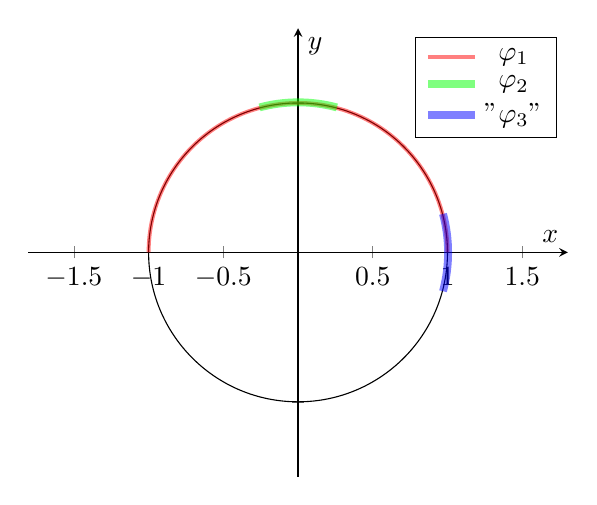
\begin{tikzpicture}
			\begin{axis}[
				axis lines = center,
				xmin=-1.5, xmax=1.5, ymin=-1.5, ymax=1.5,
				axis equal,
				xlabel = $x$,
				ylabel = {$y$},
				yticklabels={,,}
			]
			\draw (axis cs: 0, 0) circle [radius=1];
			\draw[line width=.5mm, red, opacity=.5] (axis cs: 1, 0) arc [radius=1, start angle=0, end angle=180];
			\addlegendimage{line width=.5mm, opacity=.5, color=red}
			\addlegendentry{$\varphi_1$}
			\draw[line width=1mm, green, opacity=.5] (axis cs: .26, .97) arc [radius=1, start angle=75, end angle=105];
			\addlegendimage{line width=1mm, opacity=.5, color=green}
			\addlegendentry{$\varphi_2$}
			\draw[line width=1mm, blue, opacity=.5] (axis cs: .97, -.26) arc [radius=1, start angle=-15, end angle=15];
			\addlegendimage{line width=1mm, opacity=.5, color=blue}
			\addlegendentry{"$\varphi_3$"}
			\end{axis}
		\end{tikzpicture}
		\caption{Esempi di funzioni implicite della $f$}
		\label{fig:ese_funz_impl_cerchio}
	\end{figure}
\end{example}
\begin{example}
	Posti $m = n = l = 1$
	\[\funcdef{f}{\R \times \R}{\R}{(x,y)}{x^2 + y^2}\]
	L'uguaglianza $f(x,y) = 0$ non definisce implicitamente alcuna funzione in quanto $\dom f = \brackets{(0,0)}$ che è composto da un solo punto isolato, dunque non esistono $\mathcal{X} \subseteq X$ e $\mathcal{Y} \subseteq Y$ aperti.
\end{example}
\begin{example}
	\label{ex:inf_funz_impl}
	Posti $m = n = l = 1$
	\[\funcdef{f}{\R \times \R}{\R}{(x,y)}{x^2 - y^2}\]
	L'uguaglianza $f(x,y) = 0$ definisce implicitamente infinite funzioni distinte in un intorno di $(0,0)$.
\end{example}
\begin{exercise}
	Determinare (almeno) 5 funzioni diverse definite implicitamente dalla funzione nell'\fullref{ex:inf_funz_impl} sullo stesso insieme
	% TODO solution
\end{exercise}
\begin{example}[Equazione di Keplero]
	\index{Equazione!di Keplero}
	Nella meccanica orbitale, l'\textbf{Equazione di Keplero} è un importante risultato che mette in relazione varie proprietà dell'orbita di un oggetto soggetto ad una forza centrale fornendo la legge oraria del suo moto. Dati
	\begin{itemize}[noitemsep]
		\item \makebox[2ex]{$M$\hfill} \textit{Anomalia Media}: frazione di periodo orbitale trascorsa dall'ultimo passaggio al pericentro $z$, espressa come angolo.
		\item \makebox[2ex]{$E$\hfill} \textit{Anomalia Eccentrica}: valore angolare utilizzato per correggere lo scostamento tra l'anomalia vera, cioè quella osservata, e quella media (da sopra)
		\item \makebox[2ex]{$e$\hfill} \textit{Eccentricità} dell'orbita del corpo
		\item \makebox[2ex]{$n$\hfill} \textit{Velocità angolare media} del corpo
		\item \makebox[2ex]{$t$\hfill} \textit{Istante} di tempo in cui si vuol calcolare la posizione del corpo
		\item \makebox[2ex]{$\tau$\hfill} \textit{Istante} di tempo di passaggio per il pericentro (perielio nel caso del Sole)
	\end{itemize}
	Si ha la
	\[\underbrace{E - e \sin(E)}_{= M} = n (t - \tau)\]
	Dalla quale è però impossibile esplicitare la $E$, necessaria per il calcolo della posizione, in funzione del tempo $t$. È possibile, al massimo, avvicinarsi alla soluzione con metodi di approssimazione.
\end{example}

\vspace*{\baselineskip}
Per funzioni lineari il Teorema della Funzione Implicita si riduce alla semplice inversione di una matrice.
\begin{theorem}[della Funzione Implicita - Caso Lineare]
	\index{Teorema!della Funzione Implicita - Caso Lineare}
	\label{teo:funz_impl_lin}
	Siano:
	\begin{itemize}[noitemsep]
		\item $A \in \mat(p \times n)$ matrice
		\item $B \in \mat(p \times m)$ matrice
		\item $C \in \mat(p \times 1)$ vettore colonna
		\item $p = m$
		\item $\det(B) \neq 0$
	\end{itemize}
	e la funzione
	\[\funcdef{f}{\R^n \times \R^m}{\R^p}{(x, y)}{Ax + By - C}\]
	Allora esiste un'unica funzione $\varphi: \R^n \to \R^m$ tale che:
	\[Ax + By = C \quad \iff \quad f(x,y) = 0 \quad \iff \quad y = \varphi(x)\]
	\vspace*{-5ex}
	\begin{note}
		Dimensionalmente, avendo $p = m$ ed eseguendo i prodotti righe per colonne, ci si porta ad avere da entrambi i lati dell'uguaglianza matriciale dei vettori colonna $\in \mat(p \times 1)$
	\end{note}
	\begin{proof}
		\begin{align*}
			Ax + By &= C\\
			By &= C - Ax\\
			\shortintertext{Essendo $p = m$ e $\det(B) \neq 0$, la matrice $B$ è invertibile, dunque}
			B^{-1} By &= B^{-1} (C - Ax)\\
			y &= B^{-1} (C - Ax)
		\end{align*}
		Quindi è possibile esprimere la $y$ in funzione della sola $x$, verificando la tesi.
	\end{proof}
\end{theorem}

\begin{observation}[Metodo di Newton, o delle Tangenti]~
	\index{Metodo di Newton}
	\label{obs:metodo_newton}
	\vspace*{-\baselineskip}
	\begin{note}
		Questo metodo, leggermente modificato, sarà utile nella dimostrazione del \fullref{teo:funz_impl}.
	\end{note}
	Sia $f: \intervalclose{a}{b} \to \R$ con $f \in \cntclass{2}(\intervalclose{a}{b}, \R)$. Se l'intervallo $\intervalclose{a}{b}$ contiene una sola radice della $f$, allora si può individuare la radice per mezzo di successive approssimazioni della curva con le sue tangenti.\\
	Procedendo in modo iterativo si dimostra che la relazione di ricorrenza del metodo è:
	\begin{equation}
		\label{eq:metodo_newton}
		x_{n+1} = x_n - \frac{f(x_n)}{f'(x_n)}
	\end{equation}
	Che è una successione convergente alla radice.\\
	Graficamente si vede come utilizzando le tangenti ci si possa spostare rapidamente verso la radice:
	\begin{center}
		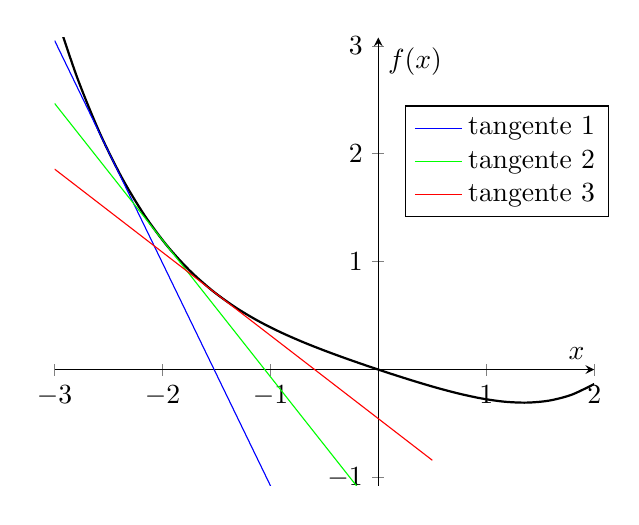
\begin{tikzpicture}[declare function = {
				curve(\x)=(1/40)*\x^4+(1/30)*\x^2-(1/3)*\x;
				derivative(\x)=(1/10)*\x^3+(1/15)*\x-(1/3);
			}]
			\begin{axis}[
				axis lines = center,
				axis equal,
				ymax = 3, ymin = -1,
				xlabel = $x$,
				ylabel = {$f(x)$},
				legend style = {at={(.65,0.6)},anchor=south west}
			]
				\addplot[domain=-3:2, smooth, thick, forget plot] {curve(x)};
				\addplot[domain=-3:.5, color=blue]{(x+2.5)*derivative(-2.5) + curve(-2.5)};
				\addlegendentry{tangente 1}
				\addplot[domain=-3:.5, color=green]{(x+2)*derivative(-2) + curve(-2)};
				\addlegendentry{tangente 2}
				\addplot[domain=-3:.5, color=red]{(x+1.5)*derivative(-1.5) + curve(-1.5)};
				\addlegendentry{tangente 3}
			\end{axis}
		\end{tikzpicture}
	\end{center}
\end{observation}

\begin{theorem}[della Funzione Implicita]~
	\index{Teorema!della Funzione Implicita}
	\label{teo:funz_impl}
	\vspace*{-\baselineskip}
	\begin{note}
		Questo teorema è anche noto come \textit{Teorema di Dini}
	\end{note}
	Siano:
	\begin{enumerate}[noitemsep]
		\item \label{itm:ipot_funz_impl_1} $X \subseteq \R^n$ e $Y \subseteq \R^m$ \textbf{Aperti}
		\item \label{itm:ipot_funz_impl_2} $f: X \times Y \to \R^m$ e $f$ \textbf{Continua} in $X \times Y$
		\item \label{itm:ipot_funz_impl_3} $(x_0, y_0) \in X \times Y$ e $f(x_0, y_0) = 0$
		\item \label{itm:ipot_funz_impl_4} $D_yf$ \textbf{esiste Continua} in $(x_0, y_0)$
		\item \label{itm:ipot_funz_impl_5} $D_yf(x_0, y_0)$ ammette \textbf{inversa}
	\end{enumerate}
	\begin{note}
		\hypertarget{note:teo_funz_impl_note_ipot1}{}
		Nel \fullref{teo:funz_impl_lin} si utilizzava direttamente la matrice dell'applicazione lineare, mentre qui si ha la matrice Derivata Totale. Questo perché il differenziale è la funzione che meglio approssima una funzione in un suo punto, permettendo una pseudo linearità malgrado la $f$ non sia (necessariamente) lineare.
	\end{note}
	\begin{note}
		Nei punti \ref{itm:ipot_funz_impl_4} e \ref{itm:ipot_funz_impl_5} delle ipotesi si ha $D_yf$ perché si sta cercando una funzione implicita che esprima la $y$, se la si stesse cercando per la $x$ si dovrebbe utilizzare la $D_xf$
	\end{note}
	\begin{note}
		Il punto \ref{itm:ipot_funz_impl_5} delle ipotesi richiede che la matrice $D_yf$ sia invertibile, cioè quadrata e con $\det(D_yf) \neq 0$. Il fatto che sia quadrata è garantito per ipotesi, in quanto $Y \subseteq \R^m$ e $f$ è a valori in $\R^m$\\
		Nel caso molto comune di $f: \R^1 \times \R^1 \to \R^1$, bisogna verificare che $\frac{\partial f}{\partial y} \neq 0$, cioè che la derivata parziale rispetto ad $y$ non sia nulla, come si vede in \fullref{coro:diff_primo_funz_impl_n1_m1}.
	\end{note}
	Allora
	\begin{enumerate}
		\item Esistono degli intorni $\mathcal{X}$ di $x_0$ e $\mathcal{Y}$ di $y_0$ ed esiste la \textbf{funzione Continua} $\varphi: \mathcal{X} \to \mathcal{Y}$ tale che, con $x \in \mathcal{X}$ e $y \in \mathcal{Y}$
			\begin{equation}
				\label{eq:teo_funz_impl_f_phi}
				f(x,y) = 0 \quad \iff \quad y = \varphi(x)
			\end{equation}
		\item \label{itm:tesi_funz_impl_1} Se $\varphi_1: \mathcal{X}_1 \to \mathcal{Y}_1$ e $\varphi_2: \mathcal{X}_2 \to \mathcal{Y}_2$ soddisfano alla \cref{eq:teo_funz_impl_f_phi} con $\mathcal{X}_1, \mathcal{X}_2 \subseteq \mathcal{X}$ intorni di $x_0$ e $\mathcal{Y}_1, \mathcal{Y}_2 \subseteq \mathcal{Y}$ intorni di $y_0$, allora
			\[\varphi_1 = \varphi_2 \quad \text{su} \quad \mathcal{X} \cap \mathcal{X}_1 \cap \mathcal{X}_2\]
			\vspace*{-1.5\baselineskip}
			\begin{note}
				Cioè, prendendo due $\varphi$ definite su intervalli diversi, esse assumeranno gli stessi valori nei punti comuni ad entrambi gli intervalli, nel caso in cui ce ne siano.\\
				Questa proprietà viene spesso indicata dalla forma "$\varphi$ è unica \textit{localmente}".
			\end{note}
	\end{enumerate}
	\begin{proof}
		Analogamente alla \cref{eq:metodo_newton}, passando al caso multidimensionale, si definisce la funzione
		\begin{equation}
			\label{eq:funz_impl_T}
			\funcdef{T}{\mathcal{X} \times \mathcal{Y}}{\mathcal{Y}}{(x,y)}{y - [D_yf(x_0, y_0)]^{-1} \cdot f(x, y)}
		\end{equation}
		\begin{note}
			$[D_yf(x_0, y_0)]^{-1}$ è la matrice inversa della $D_yf$
		\end{note}
		Considerando la $x$ della $T$ come un parametro, si può dire che $T$ sia una \fullref{def:contrazione_parametro}. Bisogna però verificare che sia effettivamente una contrazione, cioè che rispetti due condizioni:
		\begin{enumerate}
			\item \textit{La $T$ esegue una contrazione delle distanze}\\
				Questo si può dimostrare grazie al \fullref{teo:accresc_fin}. Infatti se il $\sup\limits_{\xi \in S} \norm{Df(\xi)}$ dell'\cref{eq:accresc_fin} è un numero $\in \intervalclop{0}{1}$, allora (sostituendo la distanza con la norma per \fullref{def:norma}) la \cref{eq:accresc_fin} diventa comparabile alla \cref{eq:contrazione_parametro}, cioè:
				\[
					\begin{gathered}
						d \bigl( T(x, y_1), T(x, y_2) \bigr) \leq K \cdot d(y_1, y_2)\\
						\iff\\
						\norm{ T(x, y_1) - T(x, y_2) } \leq \sup\limits_{\xi \in S} \norm{D_y T(\xi)} \cdot \norm{y_1 - y_2}
					\end{gathered}
				\]
				Per poter applicare il \fullref{teo:accresc_fin} è necessario che il segmento di estremi $y_1$, $y_2$ sia interamente contenuto nella parte interna dell'insieme di definizione di $T$.\\
				Dato che nell'enunciato del teorema è solo indicata l'esistenza di $\mathcal{X}$ e $\mathcal{Y}$, è possibile scegliere questi insiemi a piacimento. Ponendo dei $r_x$ ed $r_y$ sufficientemente piccoli, saranno accettabili:
				\[\mathcal{X} = \overline{B(x_0, r_x)} \qquad\qquad\qquad \mathcal{Y} = \overline{B(y_0, r_y)}\]
				A questo punto il \fullref{teo:accresc_fin} è applicabile, dunque si procede a quantificare il $\sup\limits_{\xi \in S} \norm{Df(\xi)}$ differenziando rispetto ad $y$ la \cref{eq:funz_impl_T}
				\begin{align*}
					D_yT(x,y) &= \id_Y - \bigl[ D_yf (x_0, y_0) \bigr]^{-1} D_yf (x, y)
					\shortintertext{Essendo $\id_Y = \bigl[ D_yf(x, y)\bigr]^{-1} \cdot D_yf(x, y)$ per qualsiasi $(x, y)$, si ha}
					&= \bigl[ D_yf (x_0, y_0) \bigr]^{-1} \cdot D_yf (x_0, y_0) - \bigl[ D_yf (x_0, y_0) \bigr]^{-1} D_yf (x, y)\\
					&= \bigl[ D_yf (x_0, y_0) \bigr]^{-1} \cdot \bigl[ D_yf (x_0, y_0) - D_yf (x, y) \bigr]
				\end{align*}
				Passando alle norme
				\[\norm{D_yT(x,y)} = \norm{\bigl[ D_yf (x_0, y_0) \bigr]^{-1} \cdot \underbrace{\bigl[ D_yf (x_0, y_0) - D_yf (x, y) \bigr]}_{\text{(1)}} }\]
				Essendo, come detto prima, $r_x$ ed $r_y$ piccoli a piacere, si può presupporre che il fattore indicato come (1) tenda a $0$, essendo una differenza tra funzioni continue (per ipotesi). A questo punto, sicuramente, si può minorare con un valore arbitrario: si sceglie $\frac{1}{2}$ in quanto sarà successivamente "comodo" nel corso della dimostrazione.
				\[\norm{D_yT(x,y)} \leq \frac{1}{2}\]
				Dunque, finalmente, applicando il \fullref{teo:accresc_fin}
				\[\norm{ T(x, y_1) - T(x, y_2) } \leq \frac{1}{2} \cdot \norm{y_1 - y_2}\]
				\qed
			\item \textit{La $T$ è a valori nell'insieme di partenza ($T$ "ben definita")}\\
				Preso un generico $y$, si deve verificare che $\forall y \in \mathcal{Y}:\; T(x,y) \in \mathcal{Y}$ cioè, per come è definito $\mathcal{Y}$, che la distanza tra $T(x,y)$ ed $y_0$, centro della $\overline{B(y_0, r_y)}$, sia minore di $r_y$.\\
				Applicando la disuguaglianza triangolare
				\begin{align*}
					\norm{T(x, y) - y_0} &\leq \norm{\underbrace{T(x, y) - T(x, y_0)}_{\text{(1)}} + \underbrace{\norm{T(x, y_0) - y_0}}_{\text{(2)}}}
					\intertext{Applicando nuovamente il \fullref{teo:accresc_fin} ad (1) ed utilizzando la definizione di $T$ per (2)}
					&\leq \underbrace{\sup\limits_{\xi \in S} \norm{D_y T(\xi)}}_{\text{(3)}} \cdot \underbrace{\norm{y - y_0}}_{\text{(4)}} + \norm{y_0 - [D_yf(x_0, y_0)]^{-1} \cdot f(x, y_0) - y_0}
					\shortintertext{Come dimostrato prima (3) è minorato da $\frac{1}{2}$, mentre (4) corrisponde a $r_y$}
					&\leq \frac{1}{2} r_y + \norm{[D_yf(x_0, y_0)]^{-1} \cdot f(x, y_0)}\\
					&= \frac{1}{2} r_y + \norm{[D_yf(x_0, y_0)]^{-1}} \cdot \norm{f(x, y_0)}\\
					&= \frac{1}{2} r_y + \norm{[D_yf(x_0, y_0)]^{-1}} \cdot \norm{f(x, y_0) - 0}
					\shortintertext{Essendo $f(x_0, y_0) = 0$ per ipotesi}
					&= \frac{1}{2} r_y + \underbrace{\norm{[D_yf(x_0, y_0)]^{-1}} \cdot \norm{f(x, y_0) - f(x_0, y_0)}}_{\text{(5)}}
					\shortintertext{Il termine (5) non dipende da $r_y$, ma solo da $r_x$, dunque scegliendo un $r_x$ sufficientemente piccolo, è possibile minorare nuovamente con}
					&\leq \frac{1}{2} r_y + \frac{1}{2} r_y\\
					&\leq r_y
				\end{align*}
				\qed
		\end{enumerate}
		Si è quindi verificato che la $T$ sia effettivamente una \textbf{Contrazione} per ogni $x \in \mathcal{X}$
		\begin{note}
			L'indipendenza dal parametro deriva dall'aver verificato la \fullref{def:contrazione_parametro}
		\end{note}
		Sfruttando il \fullref{teo:contrazioni_con_para} si può essere certi dell'unicità del punto fisso di $T$. Inoltre, il punto fisso di $T$ è anche radice di $f(x,y) = 0$. Questo si dimostra applicando la \fullref{def:punto_fisso} alla $T$:
		\begin{align*}
			T(x,y) = y \quad &\iff \quad y - [D_yf(x_0, y_0)]^{-1} \cdot f(x, y) = y\\
			&\iff \quad [D_yf(x_0, y_0)]^{-1} \cdot f(x, y) = 0
			\shortintertext{Moltiplicando ambo i membri per $D_yf$}
			&\iff \quad D_yf(x_0, y_0) \cdot [D_yf(x_0, y_0)]^{-1} \cdot f(x, y) = D_yf(x_0, y_0) \cdot 0
			\shortintertext{Una matrice moltiplicata per la sua inversa dà la matrice identità, dunque}
			&\iff \quad f(x, y) = 0
		\end{align*}
		Quindi, effettivamente, il punto fisso della $T$ è zero della $f$.\\
		È ora possibile definire una funzione che associa ad un dato parametro $x$ una $T$ in funzione di $y$ (quindi $\varphi$ è funzione di funzioni).
		\[\funcdef{\varphi}{\mathcal{X}}{\mathcal{Y}}{x}{T(x,y)}\]
		La continuità di $\varphi$ è sempre garantita da \fullref{teo:contrazioni_con_para}.
	\end{proof}
\end{theorem}
\begin{exercise}
	Confrontare le ipotesi del \fullref{teo:funz_impl_lin} e del \fullref{teo:funz_impl}.
	\begin{solution}
		Vedere \hyperlink{note:teo_funz_impl_note_ipot1}{seconda nota alle ipotesi del \fullref*{teo:funz_impl}}
	\end{solution}
\end{exercise}
\begin{exercise}
	Come mai il \fullref{teo:funz_impl} è stato ambientato in $\R^n$ e non in un generico spazio metrico?
	% TODO solution
\end{exercise}
\begin{theorem}[Differenziale Primo della Funzione Implicita]
	\index{Differenziale!Funzione Implicita!Primo}
	\label{teo:diff_primo_funz_impl}
	Nelle stesse ipotesi del \fullref{teo:funz_impl} ed aggiungendo $f \in \cntclass{1}$, allora $\varphi \in \cntclass{1}$ e vale
	\begin{equation}
		\label{eq:diff_primo_funz_impl}
		D\varphi(x) = - \Bigl[ D_yf \bigl( x, \varphi(x) \bigr) \Bigr]^{-1} \cdot D_xf \bigl( x, \varphi(x) \bigr)
	\end{equation}
	\begin{proof}
		Omessa a lezione.\\
		\cbstart
		$f$ è di classe $\cntclass{1} \quad \implies \quad f$ è Lipschitziana $\quad \implies \quad$ la funzione $T$ definita in \cref{eq:funz_impl_T} è Lipschitziana anche in $x$ (si veda \fullref{ex:comp_funz_lips}) $\quad \implies \quad$ la funzione implicita $y = \varphi(x)$ è Lipschitziana (per \fullref{teo:contr_con_para_lips_definisce_funz_lips}).

		Se $\varphi$ è derivabile, allora le regole di derivazione garantiscono che (da \fullref{ex:diff_funz_comp}):
		\[0 = D \Bigl( f \bigl( x, \varphi(x) \bigr) \Bigr) = D_xf \bigl( x, \varphi(x) \bigr) + D_yf \bigl( x, \varphi(x) \bigr)\]
		Dunque
		\[\varphi'(x) = -\Bigl( D_yf \bigl( x, \varphi(x) \bigr) \Bigr)^{-1} \cdot D_xf \bigl( x, \varphi(x) \bigr)\]
		Si pone ora per brevità
		\[A(x) = - \Bigl( D_yf \bigl( x, \varphi(x) \bigr) \Bigr)^{-1} \cdot D_xf \bigl( x, \varphi(x) \bigr)\]
		Resta dunque da verificare che
		\begin{equation}
			\label{eq:diff_primo_funz_impl_omega_x}
			\omega_x(h) = \varphi(x + h) - \varphi(x) - A(x) \cdot h \qquad \text{allora} \qquad \omega_x(h) = o(h) \text{ per } h \to 0
		\end{equation}
		Infatti
		\begin{align*}
			0 &= f \bigl( x + h, \varphi(x + h) \bigr)\\
			&= f \bigl( x + h, \varphi(x) + A(x) \cdot h + \omega_x(h) \bigr)\\
			&= D_xf \bigl( x, \varphi(x) \bigr) \cdot h + D_yf \bigl( x, \varphi(x) \bigr) \cdot \bigl( A(x) \cdot h + \omega_x(h) \bigr) + o \left( \sqrt{ \norm{h}^2 + \norm{A(x) \cdot h + \omega_x(h)}^2 } \;\; \right)\\
			&= D_yf \bigl( x, \varphi(x) \bigr) \cdot \omega_x(h) + o \left( \sqrt{ \norm{h}^2 + \norm{A(x) \cdot h + \omega_x(h)}^2 } \;\; \right)
		\end{align*}
		Quindi
		\[\omega_x(h) = \left[ D_yf \bigl( x, \varphi(x) \bigr) \right]^{-1} o \left( \sqrt{ \norm{h}^2 + \norm{A(x) \cdot h + \omega_x(h)}^2 } \;\; \right)\]
		Dalla definizione di $\omega_x$ in \cref{eq:diff_primo_funz_impl_omega_x}, segue che la funzione $h \mapsto \omega_x(h)$ è Lipschitziana (da \fullref{ex:comp_funz_lips}). Ciò implica che non possa andare a $0$ più lentamente di $h \to h$, dunque ne segue che
		\[\omega_x(h) = \left[ D_yf \bigl( x, \varphi(x) \bigr) \right]^{-1} o(\norm{h}) = o(\norm{h})\]
		\cbend
	\end{proof}
\end{theorem}
\begin{corollary}[Differenziale Primo della Funzione Implicita - Caso $n=1$, $m=1$]
	\label{coro:diff_primo_funz_impl_n1_m1}
	\index{Differenziale!Funzione Implicita!Primo - Caso $n=1$, $m=1$}
	Il \fullref{teo:diff_primo_funz_impl} nel caso caso $\boldsymbol{n=1}$, $\boldsymbol{m=1}$, la \cref{eq:diff_primo_funz_impl} diventa
	\[
		D\varphi(x) = -\frac{
			\frac{\partial f}{\partial x} \bigl( x, \varphi(x) \bigr)
		}{
			\frac{\partial f}{\partial y} \bigl( x, \varphi(x) \bigr)
		}
	\]
	\begin{proof}
		Dalla tesi del \fullref{teo:funz_impl}, si ha
		\[f(x,y) = 0 \iff y = \varphi(x)\]
		Derivando si passa alla
		\[
			\begin{gathered}
				D\Bigl( f\bigl(x,\varphi(x) \bigr) \Bigr) = 0\\
				\frac{\partial f}{\partial x}\bigl( x, \varphi(x) \bigr) + \frac{\partial f}{\partial y}\bigl( x, \varphi(x) \bigr) D\varphi(x) = 0
			\end{gathered}
		\]
		Da cui, spostando, la tesi.
	\end{proof}
\end{corollary}
\cbstart
\begin{corollary}[Differenziale Secondo della Funzione Implicita - Caso $n=1$, $m=1$]
	\index{Differenziale!Funzione Implicita!Secondo - Caso $n=1$, $m=1$}
	Nelle stesse ipotesi del \fullref{teo:funz_impl} ed aggiungendo $f \in \cntclass{2}$, allora $\varphi \in \cntclass{2}$ e vale
	\begin{equation}
		\label{eq:diff_sec_funz_impl}
		D^2\varphi(x) = -
		\frac{
			\frac{\partial^2 f}{\partial x \partial x} (\dots)
			\left[ \frac{\partial f}{\partial y} (\dots) \right]^2 -
			2 \frac{\partial f}{\partial x} (\dots)
			\frac{\partial f}{\partial y} (\dots)
			\frac{\partial^2 f}{\partial x \partial y} (\dots) +
			\frac{\partial^2 f}{\partial y \partial y} (\dots)
			\left[ \frac{\partial f}{\partial x} (\dots) \right]^2
		}{
			\left[ \frac{\partial f}{\partial y} (\dots) \right]^3
		}
	\end{equation}
	\begin{note}
		Gli argomenti $(\dots)$ delle funzioni nella \cref{eq:diff_sec_funz_impl} stanno per $\bigl( x, \varphi(x) \bigr)$.
	\end{note}
	\begin{note}
		Si noti che in questa formula compaiono derivate seconde e derivate prime (anche elevate al quadrato). È necessario far attenzione nello svolgimento.
	\end{note}
	\begin{proof}
		Omessa. Il seguente svolgimento è riportato solamente allo scopo di facilitare la memorizzazione del processo per ricavare la formula di cui sopra.
		Si inizia derivando ulteriormente il risultato di \fullref{coro:diff_primo_funz_impl_n1_m1}.
		\begin{gather*}
			D^2 \varphi(x) =
			D \left[ - \frac{
				\frac{\partial f}{\partial x} \bigl( x, \varphi(x) \bigr)
			}{
				\frac{\partial f}{\partial y} \bigl( x, \varphi(x) \bigr)
			} \right] =
			\shortintertext{Usando la nota regola di derivazione del rapporto di funzioni}
			- \frac{
				D \left[ \frac{\partial f}{\partial x} \bigl( x, \varphi(x) \bigr) \right] \;
				\frac{\partial f}{\partial y} \bigl( x, \varphi(x) \bigr) -
				\frac{\partial f}{\partial x} \bigl( x, \varphi(x) \bigr) \;
				D \left[ \frac{\partial f}{\partial y} \bigl( x, \varphi(x) \bigr) \right]
			}{
				\left[ \frac{\partial f}{\partial y} (\dots) \right]^2
			} =
			\shortintertext{Posto ora per brevità $(\dots) = \bigl( x, \varphi(x) \bigr)$}
			- \frac{
				\left[
					\frac{\partial^2 f}{\partial x \partial x} (\dots) +
					D\varphi(x) \;
					\frac{\partial^2 f}{\partial x \partial y} (\dots)
				\right]
				\frac{\partial f}{\partial y} (\dots) -
				\frac{\partial f}{\partial x} (\dots)
				\left[
					\frac{\partial^2 f}{\partial y \partial x} (\dots) +
					D\varphi(x) \;
					\frac{\partial^2 f}{\partial y \partial y} (\dots)
				\right]
			}{
				\left[ \frac{\partial f}{\partial y} (\dots) \right]^2
			} =
			\shortintertext{Sostituendo infine $D\varphi(x)$ con quanto ottenuto in \fullref{coro:diff_primo_funz_impl_n1_m1}}
			- \frac{
				\left[
					\frac{\partial^2 f}{\partial x \partial x} (\dots) -
					\frac{
						\frac{\partial f}{\partial x} (\dots)
					}{
						\frac{\partial f}{\partial y} (\dots)
					} \;
					\frac{\partial^2 f}{\partial x \partial y} (\dots)
				\right]
				\frac{\partial f}{\partial y} (\dots) -
				\frac{\partial f}{\partial x} (\dots)
				\left[
					\frac{\partial^2 f}{\partial y \partial x} (\dots) -
					\frac{
						\frac{\partial f}{\partial x} (\dots)
					}{
						\frac{\partial f}{\partial y} (\dots)
					} \;
					\frac{\partial^2 f}{\partial y \partial y} (\dots)
				\right]
			}{
				\left[ \frac{\partial f}{\partial y} (\dots) \right]^2
			} =\\
			- \frac{
				\frac{\partial^2 f}{\partial x \partial x} (\dots) \; \frac{\partial f}{\partial y} (\dots) -
				%
				\frac{
					\frac{\partial f}{\partial x} (\dots)
				}{
					\cancel{\frac{\partial f}{\partial y} (\dots)}
				} \;
				\frac{\partial^2 f}{\partial x \partial y} (\dots) \;
				\cancel{\frac{\partial f}{\partial y} (\dots)} -
				%
				\frac{\partial f}{\partial x} (\dots) \; \frac{\partial^2 f}{\partial y \partial x} (\dots) +
				%
				\frac{\partial f}{\partial x} (\dots) \;
				\frac{
					\frac{\partial f}{\partial x} (\dots)
				}{
					\frac{\partial f}{\partial y} (\dots)
				} \;
				\frac{\partial^2 f}{\partial y \partial y} (\dots)
			}{
				\left[ \frac{\partial f}{\partial y} (\dots) \right]^2
			} =
			\shortintertext{Sfruttando ora il \fullref{lemma:schwarz}}
			- \frac{
				\frac{\partial^2 f}{\partial x \partial x} (\dots) \; \frac{\partial f}{\partial y} (\dots) -
				%
				2 \frac{\partial f}{\partial x} (\dots) \; \frac{\partial^2 f}{\partial x \partial y} (\dots) +
				%
				\frac{
					\left[ \frac{\partial f}{\partial x} (\dots) \right]^2
				}{
					\frac{\partial f}{\partial y} (\dots)
				} \;
				\frac{\partial^2 f}{\partial y \partial y} (\dots)
			}{
				\left[ \frac{\partial f}{\partial y} (\dots) \right]^2
			} =
			\shortintertext{Forzando ora il raccoglimento di $\frac{\partial f}{\partial y} (\dots)$ si giunge alla tesi}
			- \frac{
				\frac{\partial^2 f}{\partial x \partial x} (\dots) \; \left[ \frac{\partial f}{\partial y} (\dots) \right]^2 -
				%
				2 \frac{\partial f}{\partial x} (\dots) \;
				\frac{\partial^2 f}{\partial x \partial y} (\dots) \;
				\frac{\partial f}{\partial y} (\dots) +
				%
				\left[ \frac{\partial f}{\partial x} (\dots) \right]^2 \;
				\frac{\partial^2 f}{\partial y \partial y} (\dots)
			}{
				\left[ \frac{\partial f}{\partial y} (\dots) \right]^3
			}
		\end{gather*}
	\end{proof}
\end{corollary}
\cbend
\begin{exercise}
	\label{ex:funz_impl_diff_k}
	Tramite la \cref{eq:diff_primo_funz_impl} dimostrare che se $f$ soddisfa le ipotesi del \fullref{teo:funz_impl} ed è di classe $\cntclass{k}$, allora anche la \textbf{Funzione Implicita} è di classe $\cntclass{k}$.
	% TODO solution
\end{exercise}
\begin{example}
	L'uguaglianza $y^3 = x^6$ definisce un'unica funzione implicita $y = y(x)$ in un intorno di $(0,0)$, pur non soddisfacendo alle ipotesi del \fullref{teo:funz_impl}.
\end{example}
\begin{example}
	Data una funzione $f \in \cntclass{1}(\R^2;\R)$, il luogo geometrico descritto da $f(x,y) = 0$ coincide con quello descritto da $\bigl( f(x,y) \bigr)^2 = 0$, ma anche se la prima equazione soddisfa alle ipotesi del \fullref{teo:funz_impl}, la seconda sicuramente non lo fa.
\end{example}
\begin{example}
	Entrambe le funzioni

	\vspace*{\baselineskip}
	\begin{minipage}{0.48\linewidth}
		\[\funcdef{f}{\R^3}{\R^2}{(x,y,z)}{(x,y)}\]
	\end{minipage}
	\begin{minipage}{0.48\linewidth}
		\[\funcdef{f}{\R^3}{\R}{(x,y,z)}{x^2+y^2}\]
	\end{minipage}

	\vspace*{\baselineskip}
	\noindent descrivono l'asse $z$ attraverso le equazioni

	\vspace*{\baselineskip}
	\begin{minipage}{0.48\linewidth}
		\[f(x,y,z) = 0\]
	\end{minipage}
	\begin{minipage}{0.48\linewidth}
		\[g(x,y,z) = 0\]
	\end{minipage}

	\vspace*{\baselineskip}
	\noindent Tuttavia, mentre $f$ soddisfa alle ipotesi del \fullref{teo:funz_impl}, la $g$ le soddisfa.\\
	Grazie al citato teorema, la $f$ (nell'intorno di un qualsiasi punto $(0,0,z)$) definisce sicuramente una funzione implicita $(x,y) = \varphi(z)$ data da $\varphi(z) = 0$.
	\begin{note}
		L'esempio precedente mostra come, ai fini della determinazione del numero di gradi di libertà di un sistema, possa essere fuorviante fare affidamento sul numero di equazioni che identificano il vincolo
	\end{note}
\end{example}
\begin{corollary}
	Siano
	\begin{itemize}[noitemsep]
		\item $A \subseteq \R^n$
		\item $x_0 \in \circdot{A}$
		\item $f \in \cntclass{1}(A;\R^m)$
		\item $f(x_0) = 0$
		\item $n > m$
	\end{itemize}
	Se $Df(x_0)$ ha rango $m$, il vincolo implicito $f(x) = 0$ equivale ad una relazione esplicita in cui $n - m$ variabili dipendono dalle rimanenti $m$.
	\begin{proof}
		Applicare il \fullref{teo:funz_impl} % TODO proper proof
	\end{proof}
\end{corollary}
\begin{exercise}
	Studiare il luogo dei punti in cui le coordinate soddisfano a $y + xe^y = x$ in intorni di $(-1,0)$, $(0,0)$ e $(1,0)$.\\
	Tracciarne il grafico globale.
	% TODO solution
\end{exercise}

\subsection{Il Teorema della Funzione Inversa}
Data una funzione $f$, poterla invertire significa poter risolvere in un unico modo l'equazione (o sistema) $f(x) = y$ determinando l'incognita $x$ in funzione del parametro $y$, cioè ottenere $x = f^{-1}(y)$.
\begin{theorem}[della Funzione Inversa - Caso Lineare]
	\index{Teorema!della Funzione Inversa - Caso Lineare}
	\index{Funzione!Inversa}
	Sia $f: \R^n \to \R^m$ data da $f(x) = Mx$ e $ M \in \mat(m\times n)$
	\[f \text{ è invertibile} \quad \iff \quad n = m \text{ e } \det M \ne 0\]
	\begin{proof}
		Dalle nozioni di Algebra Lineare
		\begin{align*}
			X \cdot A &= Y\\
			A^{-1} \cdot X \cdot A &= A^{-1} \cdot Y\\
			X &= A^{-1} \cdot Y
		\end{align*}
	\end{proof}
\end{theorem}
\begin{theorem}[della Funzione Inversa]
	\index{Teorema!della Funzione Inversa}
	\label{teo:funz_inv}
	Siano
	\begin{itemize}[noitemsep]
		\item $X \subseteq \R^n$ è \textbf{Aperto}
		\item $x_0 \in X$
		\item $f \in \cntclass{k}(X;\R^n)$ con $k \geq 1$
		\item $Df(x_0)$ \textbf{Invertibile}
	\end{itemize}
	\begin{note}
		Perché una matrice sia Invertibile è richiesto che:
		\begin{itemize}[nolistsep]
			\item sia quadrata - vero per ipotesi, essendo $f: \R^{\boldsymbol{n}} \to \R^{\boldsymbol{n}}$
			\item $\det Df(x_0) \neq 0$ - \textbf{da verificare} caso per caso
		\end{itemize}
	\end{note}
	Allora esiste un \textbf{Aperto} $\mathcal{X} \subseteq X$ tale che:
	\begin{itemize}[noitemsep]
		\item $x_0 \in \mathcal{X}$
		\item $f(\mathcal{X})$ è un \textbf{aperto}
		\item $f_{|\mathcal{X}}: \mathcal{X} \to f(\mathcal{X})$ è \textbf{Invertibile} e l'inversa è $\cntclass{k}$
		\item $(Df^{-1})(y) = \Bigl[Df\bigl( f^-1(y) \bigr)\Bigr]^{-1}$
	\end{itemize}
	\begin{note}
		$f_{|\mathcal{X}}$ è la \textbf{Restrizione} di $f$ ai soli elementi di $\mathcal{X}$
	\end{note}
	\begin{proof}
		Sia $\Omega = \brackets{x \in X: \det Df(x) \neq 0}$ l'insieme di tutti i punti in cui la $Df(x)$ è invertibile. Per ipotesi sicuramente $\Omega$ è aperto, essendo $X$ aperto, e $x_0 \in \Omega$.
		Posta ora $F$
		\[\funcdef{F}{\Omega \times \R^n}{\R^n}{x, y}{f(x) - y}\]
		Si va a verificare che la $F$ rispetti le ipotesi del \fullref{teo:funz_impl}, modificando però le ipotesi per far riferimento alla $D_xf$:
		\begin{enumerate}[noitemsep]
			\item[\ref{itm:ipot_funz_impl_1}.] è verificato perché $\Omega$ aperto, come detto, ed $\R^n$ è aperto a sua volta
			\item[\ref{itm:ipot_funz_impl_2}.] è verificato perché $F$ somma di funzioni continue nell'intervallo scelto
			\item[\ref{itm:ipot_funz_impl_3}.] Dalla definizione di $F$, $F(x_0, y_0) = 0 \iff y_0 = f(x_0)$
			\item[\ref{itm:ipot_funz_impl_4}.] è verificato per ipotesi
			\item[\ref{itm:ipot_funz_impl_5}.] è verificato per definizione dell'insieme $\Omega$. $D_xF(x,y) = Df(x)$ perché, derivando parzialmente rispetto ad $x$, la derivata di $y$ è $0$, essendo $y$ assimilabile ad una costante.
		\end{enumerate}
		Esiste dunque una funzione $\varphi: I \to J$, con $I$ intorno di $y_0$ e $J$ intorno di $x_0$, tale che:
		\begin{equation}
			\label{eq:teo_funz_inv_applicaz_funz_impl}
			\underbrace{
				x = \varphi(y)
				\quad \iff \quad
				F(x,y) = 0
			}_{
				\mathclap{
					\text{
							\begin{tabular}{c}
								Per\\[-1ex]
								\fullref{teo:funz_impl}
							\end{tabular}
						}
				}
			}
			\quad
			\overset{
				\mathclap{
					\rule[-\baselineskip]{0pt}{\baselineskip}
					\text{
						\begin{tabular}{c}
							Riportandosi\\[-1ex]
							alla $f$
						\end{tabular}
					}
				}
			}{\iff}
			\quad
			y =f(x)
		\end{equation}

		\begin{note}
			Nella \cref{eq:teo_funz_inv_applicaz_funz_impl} è stato applicato il \fullref{teo:funz_impl} rispetto alla variabile $x$, diversamente da quanto fatto nell'enunciato del teorema stesso, dove la derivata in questione era la $y$.
		\end{note}
		Dunque, con il primo e l'ultimo elemento
		\begin{equation}
			\label{eq:teo_funz_inv_f_phi}
			x = \varphi(y) \iff y =f(x)
		\end{equation}
		È ora necessario individuare l'insieme su cui $f$ è invertibile. Si pone $\mathcal{X} = f^{-1}(I) \cap J$ dove:
		\begin{itemize}[noitemsep]
			\item $f^{-1}(I)$ è l'insieme controimmagine di $f$, cioè "tutti i valori di cui si può calcolare la $f$"
			\item $J$ è l'insieme immagine della $\varphi$, quindi "i valori delle $x$ in funzione delle $y$"
		\end{itemize}
		\begin{note}
			Vedere \fullref{ex:funz_inv_ma_non_iniett} per capire come $f^{-1}(I)$ possa essere diverso da $J$
		\end{note}
		Avendo eseguito l'intersezione, si ha la certezza che nei punti di $\mathcal{X}$, la $f$ sia invertibile e che la $\varphi$ assuma valori validi. Data la relazione tra $f$ e $\varphi$ trovata in \cref{eq:teo_funz_inv_f_phi}, si può concludere che, per i valori in $\mathcal{X}$, la $f$ è sicuramente invertibile e la sua inversa è $\varphi$.

		Inoltre $F$ è funzione di classe $\cntclass{k}$, essendo somma di $f \in \cntclass{k}$ $y \in \cntclass{\infty}$. Son dunque verificate anche le ipotesi del \fullref{teo:diff_primo_funz_impl} (ed \fullref{ex:funz_impl_diff_k}), ciò implica che $\varphi$ sia di classe $\cntclass{k}$.

		Infine si ottiene la regola di derivazione:
		\begin{align*}
			(Df^{-1})(y) &= D\varphi(y)
			\shortintertext{Dal \fullref{teo:diff_primo_funz_impl}}
			&= -\Bigl[ D_xF \bigl( \varphi(y), y \bigr) \Bigr]^{-1} \cdot D_yF \bigl( \varphi(y), y \bigr)
			\shortintertext{Per definizione di $F$, la derivata parziale rispetto a $y$ è una costante, cioè la matrice identità}
			&= -\Bigl[ D_xF \bigl( \varphi(y), y \bigr) \Bigr]^{-1} \cdot (-\id)\\
			&= -\Bigl[ D_xF \bigl( \varphi(y), y \bigr) \Bigr]^{-1}
		\end{align*}
	\end{proof}
\end{theorem}
\begin{example}~
	\label{ex:funz_inv_ma_non_iniett}
	\vspace*{-\baselineskip}
	\begin{note}
		Questo esempio mostra come il \fullref{teo:funz_inv} non possa essere applicato globalmente, ma solo in intorni. Il fatto che il Teorema valga localmente in tutto il dominio della $f$ \textbf{non implica} valga globalmente.
	\end{note}
	Sia
	\[\funcdef{f}{\R^2}{\R^2}{(x,y)}{(e^x \cos y, e^x \sin y)}\]
	La $f$ è di classe $\cntclass{\infty}$ ed inoltre $Df(x,y)$ è invertibile per ogni coppia $(x,y) \in \R^2$, quindi il \fullref{teo:funz_inv} può essere applicato in ogni $(x_0, y_0) \in \R^2$\\
	$f$ però non è globalmente invertibile, infatti non è iniettiva, ma è $2\pi$-periodica nella variabile $y$.
	\begin{note}
		La $f$ può anche essere scritta come $f(z)) = e^z$, come da \fullref{def:exp_complesso}.
	\end{note}
\end{example}
\begin{exercise}~
	\vspace*{-\baselineskip}
	\begin{note}
		Questo esempio mostra come il \fullref{teo:funz_inv} offra una condizione sufficiente a garantire l'invertibilità, ma non necessaria.
	\end{note}
	Sia
	\[\funcdef{f}{\R}{\R}{x}{x^3}\]
	$f$ è invertibile con inversa continua, malgrado sia $f'(0) = 0$.
\end{exercise}
\begin{exercise}
	Date due qualunque funzioni $f \in \cntclass{1}(\R^2;\R)$ e $g \in \cntclass{1}(\R;\R^2)$, verificare che alla funzione $g \circ f$ non può essere applicato il \fullref{teo:funz_inv}.\\
	Esibire un esempio di funzioni $f \in \cntclass{1}(\R^2;\R)$ e $g \in \cntclass{1}(\R;\R^2)$ tali che la funzione $f \circ g$ invece soddisfi le ipotesi del \fullref{teo:funz_inv}.
	% TODO solution
\end{exercise}
\begin{exercise}
	La funzione $f \in \cntclass{1}(\R^n;\R)$ soddisfa alle ipotesi del \fullref{teo:funz_inv} in $x_0$ e la funzione $g \in \cntclass{1}(\R^n; \R^n)$ soddisfa alle ipotesi del \fullref{teo:funz_inv} in $f(x_0)$. Verificare che la funzione $g \circ f$ soddisfa alle ipotesi del \fullref{teo:funz_inv} in $x_0$.
	% TODO solution
\end{exercise}

\newpage
\section{Massimi e Minimi Liberi}
\begin{definition}[Massimi e Minimi]
	\index{Massimo di una Funzione}\index{Minimo di una Funzione}
	\index{Punto!di Massimo}\index{Punto!di Minimo}
	\label{def:max_min}
	Siano $(X,d)$ uno \textbf{Spazio Metrico}, $A \subseteq X$, $x_0 \in A$ e $f: A \to \R$. Con $B \subseteq A$ e $m, M \in \R$, si dicono:
	\begin{itemize}
		\item \makebox[20em][l]{$M$ è il \textbf{Massimo} di $f$ su $B$}
			$\bydef \quad M = \max f(B)$
		\item \makebox[20em][l]{$m$ è il \textbf{Minimo} di $f$ su $B$}
			$\bydef \quad m = \min f(B)$
		\item \makebox[20em][l]{$x_0$ punto di \textbf{Massimo Assoluto} per $f$}
			$\bydef \quad f(x_0) = \max\limits_{A} f$
		\item \makebox[20em][l]{$x_0$ punto di \textbf{Minimo Assoluto} per $f$}
			$\bydef \quad f(x_0) = \min\limits_{A} f$
		\item \makebox[20em][l]{$x_0$ punto di \textbf{Massimo Locale} per $f$}
			$\bydef \quad \begin{cases}
				\exists r > 0:\; \forall x \in B(x_0,r) \cap A\\
				f(x_0) \geq f(x)
			\end{cases}$
		\item \makebox[20em][l]{$x_0$ punto di \textbf{Minimo Locale} per $f$}
			$\bydef \quad \begin{cases}
				\exists r > 0:\; \forall x \in B(x_0,r) \cap A\\
				f(x_0) \leq f(x)
			\end{cases}$
		\item \makebox[20em][l]{$x_0$ punto di \textbf{Massimo Locale Forte} per $f$}
			$\bydef \quad \begin{cases}
				\exists r > 0:\; \forall x \in B(x_0,r) \cap A \text{ con } x \neq x_0\\
				f(x_0) > f(x)
			\end{cases}$
		\item \makebox[20em][l]{$x_0$ punto di \textbf{Minimo Locale Forte} per $f$}
			$\bydef \quad \begin{cases}
				\exists r > 0:\; \forall x \in B(x_0,r) \cap A \text{ con } x \neq x_0\\
				f(x_0) < f(x)
			\end{cases}$
		\item \makebox[20em][l]{$x_0$ di \textbf{Estremo} per $f$}
			$\bydef \quad x_0$ punto di \textbf{Massimo} o di \textbf{Minimo}
	\end{itemize}
	\begin{note}
		I punti di massimo/minimo son anche indicati con $\arg \max f$ e $\arg \min f$
	\end{note}
	\begin{note}
		A volte si parla di estremi (Massimi/Minimi) \textbf{Relativi} come sinonimi di estremi \textbf{Locali}.
	\end{note}
\end{definition}
\begin{observation}
	\label{obs:inf_pti_max_min_abs}
	Una funzione ha \textbf{unico massimo/minimo}, ma può avere \textbf{infiniti punti di massimo/minimo assoluto}.
	\begin{itemize}
		\item Un estremo di $f$ ($\max f$ o $\min f$) è un punto in $\R$, insieme di arrivo della $f$, ed è il valore massimo o minimo assunto dalla $f$ stessa. È unico per definizione di $\max$ e $\min$.
		\item Un punto di estremo assoluto $x_0$ è un punto in $A$, insieme di partenza della $f$, per cui $f$ assume il suo valore massimo o minimo.
	\end{itemize}
	La non unicità dei \textit{punti di estremo} non è in conflitto con l'unicità degli \textit{estremi}, in quanto possono esistere diversi $x_1, x_2,\:\dotsc\: x_n$ per cui,ad esempio, $f(x_i) = \max f$, ma $\max f$ è sempre lo stesso.\\
	Vedere \fullref{ex:f_con_inf_pti_max_min_abs} e \fullref{ex:uniq_max_min_abs}.
\end{observation}
\newpage % WARNING Check this is not generating too much whitespace
\begin{exercise}
	Formulare le definizioni di Massimo/Minimo Assoluto Forte e di Estremo Locale/Assoluto Forte e non.
	\begin{solution}\leavevmode
		\begin{itemize}
			\item \makebox[21em][l]{$x_0$ punto di \textbf{Massimo Assoluto Forte} per $f$}
				$\bydef \quad \forall x \in A \;\; f(x_0) > f(x)$
			\item \makebox[21em][l]{$x_0$ punto di \textbf{Minimo Assoluto Forte} per $f$}
				$\bydef \quad \forall x \in A \;\; f(x_0) < f(x)$
		\end{itemize}
		\begin{note}
			Queste due definizioni son diverse rispetto a quelle dei punti di Massimo/Minimo Assoluto date in \fullref{def:max_min} perché ora si implica unicità di $x_0$.
		\end{note}
		\begin{itemize}
			\item \makebox[21em][l]{$x_0$ punto di \textbf{Estremo Locale} per $f$}
				$\bydef \quad
				\begin{cases}
					\begin{array}{c}
						\text{Unione delle definizioni di}\\[-1ex]
						\text{\textbf{Massimo Locale}}\\[-1ex]
						e\\[-1ex]
						\text{\textbf{Minimo Locale}}
					\end{array}
				\end{cases}$
			\item \makebox[21em][l]{$x_0$ punto di \textbf{Estremo Locale Forte} per $f$}
				$\bydef \quad
				\begin{cases}
					\begin{array}{c}
						\text{Unione delle definizioni di}\\[-1ex]
						\text{\textbf{Massimo Locale Forte}}\\[-1ex]
						e\\[-1ex]
						\text{\textbf{Minimo Locale Forte}}
					\end{array}
				\end{cases}$
			\item \makebox[21em][l]{$x_0$ punto di \textbf{Estremo Assoluto} per $f$}
				$\bydef \quad
				\begin{cases}
					\begin{array}{c}
						\text{Unione delle definizioni di}\\[-1ex]
						\text{\textbf{Massimo Assoluto}}\\[-1ex]
						e\\[-1ex]
						\text{\textbf{Minimo Assoluto}}
					\end{array}
				\end{cases}$
			\item \makebox[21em][l]{$x_0$ punto di \textbf{Estremo Assoluto Forte} per $f$}
				$\bydef \quad
				\begin{cases}
					\begin{array}{c}
						\text{Unione delle definizioni di}\\[-1ex]
						\text{\textbf{Massimo Assoluto Forte}}\\[-1ex]
						e\\[-1ex]
						\text{\textbf{Minimo Assoluto Forte}}
					\end{array}
				\end{cases}$
		\end{itemize}
	\end{solution}
\end{exercise}
\begin{exercise}
	Esibire esempi di funzioni con infiniti punti di massimo/minimo assoluti.
	\begin{solution}
		\begin{align*}
			f(x) &= 1 &f(x) &= \sin(x)
		\end{align*}
	\end{solution}
\end{exercise}
\begin{exercise}
	\label{ex:f_con_inf_pti_max_min_abs}
	Esibire esempi di funzioni con infiniti punti di massimo/minimo assoluti e prive di minimo/massimo assoluti.
	\begin{note}
		Notare che son richiesti infiniti \textbf{punti} di massimo/minimo, come da \fullref{obs:inf_pti_max_min_abs}.
	\end{note}
	\begin{solution}\hfill\\
		\vspace*{\baselineskip}
		\begin{minipage}{0.49\linewidth}
			\begin{center}
				$f(x) = \abs{\tan(x)}$ ha infiniti punti di minimo assoluto,\\
				ma ovviamente unico minimo assoluto $\min f = 0$
			\end{center}
		\end{minipage}
		\begin{minipage}{0.49\linewidth}
			\begin{center}
				$f(x,y) = -\sqrt{x^2+y^2-1}$ ha dominio $U = \brackets{(x, y) \in \R^2:\; x^2 + y^2 > 1}$.\\
				La $f$ ha infiniti punti di massimo assoluto in $\partial U = \brackets{(x, y) \in \R^2:\; x^2 + y^2 = 1}$,\\
				ma ovviamente unico massimo assoluto $\max f = 0$
			\end{center}
		\end{minipage}\\
		\vspace*{\baselineskip}
		\begin{minipage}{0.49\linewidth}
			\begin{center}
				\resizebox{\linewidth}{!}{
					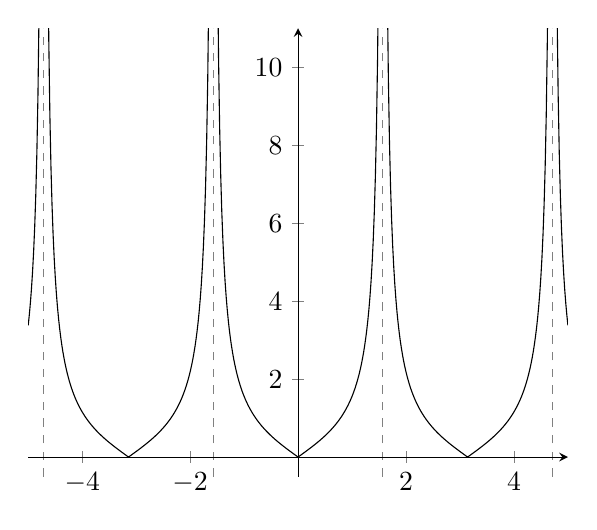
\begin{tikzpicture}
						\begin{axis} [
							axis lines = center,
							axis on top=true,
							ymax = 11, ymin = -.5
						]
							% Restricting y fixes spurious lines being generated by Adobe Acrobat when printing the graph
							% Also, y domain is a bit bigger than the displayed graph since otherwise the functions wouldn't be properly plotted
							\addplot [domain=-5:5, restrict y to domain=0:15, samples=500] {abs(tan(deg(x)))};
							\draw [dashed, color=black!50] (axis cs:pi/2,-.5) -- (axis cs:pi/2,11);
							\draw [dashed, color=black!50] (axis cs:3*pi/2,-.5) -- (axis cs:3*pi/2,11);
							\draw [dashed, color=black!50] (axis cs:-pi/2,-.5) -- (axis cs:-pi/2,11);
							\draw [dashed, color=black!50] (axis cs:-3*pi/2,-.5) -- (axis cs:-3*pi/2,11);
						\end{axis}
					\end{tikzpicture}
				}
			\end{center}
		\end{minipage}
		\begin{minipage}{0.49\linewidth}
			\begin{center}
				\resizebox{\linewidth}{!}{
					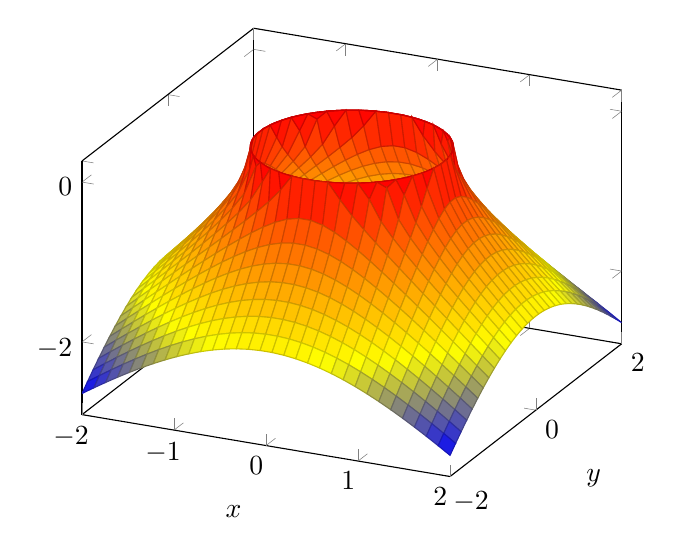
\begin{tikzpicture}
						% Thanks to Symbol 1 from https://tex.stackexchange.com/a/543874/206062
						\pgfmathdeclarefunction{volcano_z}{2}{%
							\pgfmathsetmacro\radsq{#1^2 + #2^2}% \radsq is radius^2 in FPU notation
							\pgfmathfloattofixed{\radsq}\let\radsqsafe=\pgfmathresult % in safe notation
							\ifdim\radsqsafe pt > 1pt\relax
								\pgfmathparse{-sqrt(\radsq-1)}%
							\else\ifdim\radsqsafe pt > 0.25pt\relax
								\pgfmathparse{+0}%
							\else % \radsq pt <= 0.25
								\pgfmathparse{NaN}%
							\fi\fi
						}
						\pgfmathdeclarefunction{volcano_x}{2}{%
							\pgfmathsetmacro\radsq{#1^2 + #2^2}% \radsq is radius^2 in FPU notation
							\pgfmathfloattofixed{\radsq}\let\radsqsafe=\pgfmathresult % in safe notation
							\ifdim\radsqsafe pt > 1pt\relax
								\pgfmathparse{#1}%
							\else\ifdim\radsqsafe pt > 0.25pt\relax
								\pgfmathparse{#1/sqrt(\radsq)}%
							\else % \radsq pt <= 0.25
								\pgfmathparse{NaN}%
							\fi\fi
						}
						\begin{axis}[
							xlabel=$x$, ylabel=$y$,
							]
							\addplot3[surf,domain =-2:2,unbounded coords=jump,samples=32]
								({volcano_x(x,y)}, {volcano_x(y,x)}, {volcano_z(x,y)});
						\end{axis}
					\end{tikzpicture}
				}
			\end{center}
		\end{minipage}
	\end{solution}
\end{exercise}
\begin{exercise}
	\index{Estremo Superiore/Inferiore di un Insieme}
	\index{Unicità!Massimi e Minimi Assoluti}
	\label{ex:uniq_max_min_abs}
	Formulare e dimostrare l'\textbf{unicità} del Massimo/Minimo Assoluto.
	\begin{note}
		Notare che è richiesta l'unicità del \textit{massimo/minimo assoluto}, non dei \textit{punti di massimo/minimo}. Si ricorda l'\fullref{obs:inf_pti_max_min_abs}.
	\end{note}
	\begin{solution}
		Si definisce un punto $x = \max X$, \textit{Massimo} di un insieme, quando $x = \sup X$ e $x \in X$.\\
		Essendo $x = \sup X$, dalla definizione di $\sup$, \textit{Estremo Superiore}, segue che $x$ sia il più piccolo dei maggioranti di $X$. L'unicità del $\sup$ si dimostra per assurdo:
		\begin{proof}
			\renewcommand\qedsymbol{$\square$} % To restore the default empty square for this proof environment
			Dati $A \subseteq \R$ e $B \subseteq A$, si supponga esistano $M_1, M_2 \in A$ con $M_1 \neq M_2$, due $\sup$ diversi dell'insieme $B$. Applicando la definizione di maggiorante:
			\[\forall x \in B,\; x \leq M_1 \qquad \text{e} \qquad \forall x \in B,\; x \leq M_2\]
			Si può ora supporre che sia $M_1 > M_2$ senza perdere generalità, però questo significa che $M_1$ non sia $\sup$, (non è il più piccolo dei maggioranti), negando l'ipotesi - \textit{Assurdo}
		\end{proof}
		Per come è definito dunque, anche il $\max$ sarà unico, da cui la tesi.
	\end{solution}
\end{exercise}
\begin{exercise}
	\label{ex:max_min_lib_funz_in_R}
	In questa sezione compaiono esclusivamente funzioni a valori in $\R$. Perché?
	\begin{solution}
		Perché si stanno considerando i valori assunti dalla $f$ come punti nello spazio (nella retta reale, essendo in $\R$) e non esistono necessariamente relazioni d'ordine in altri insiemi. Non è possibile ad esempio stabilire se un punto punto sia "maggiore o minore" di un altro in $\R^2$ o in $\C$.
	\end{solution}
\end{exercise}

\subsection{Condizioni Necessarie}
Le seguenti condizioni permettono di identificare dei punti \textit{potenzialmente} estremanti, ma sarà poi necessario verificare che effettivamente lo siano studiando la funzione in un loro intorno.
\begin{proposition}
	\label{prop:f_deriv_pto_estr_deriv_direz_nulla}
	Siano $A \subseteq \R^n$, $x_0 \in \circdot{A}$, $f: A \to \R$ e $v \in \R^n \setminus \brackets{0}$, allora
	\[
		\left.
			\begin{array}{c}
				f \text{ \textbf{Derivabile} in } x_0 \text{ lungo } v\\
				x_0 \text{ punto \textbf{di estremo} per } f
			\end{array}
		\right\}
		\quad \implies \quad
		D_vf(x_0) = 0
	\]
	\begin{proof}
		Se $x_0$ è di estremo per $f$, allora, scelto un opportuno $\delta > 0 \in \R$, $x_0$ è di estremo anche per la funzione
		\[\funcdef{\varphi}{\intervalopen{-\delta}{\delta}}{\R}{t}{f(x_0 + tv)}\]
		La $\varphi$ è una funzione reale di variabile reale e derivabile in $0$ perché $f$ è derivabile per ipotesi. Ciò significa che è possibile applicare alla $\varphi$ il \textit{Teorema di Fermat} di Analisi 1, avendo la garanzia che in un punto estremante di questa funzione sia $\varphi'(x_0) = 0$.\\
		Applicando ora la definizione di derivata di Analisi 1 si ottiene:
		\[
			\varphi'(t) = \lim\limits_{h \to 0} \frac{\varphi(t + h) - \varphi(t)}{h}
		\]
		Se si calcola la derivata di $\varphi$ nel punto $0$ ($\varphi(0) = f(x_0)$, con $x_0$ estremante per ipotesi) si ottiene:
		\begin{align*}
			0 &= \varphi'(0)\\
			&= \lim\limits_{h \to 0} \frac{\varphi(h) - \varphi(0)}{h}
			\shortintertext{Ma, essendo $\varphi(h) = f(x_0 + hv)$ e $\varphi(0) = f(x_0)$}
			&= \lim\limits_{h \to 0} \frac{f(x_0 + hv) - f(x_0)}{h} \tageq\label{eq:estr_f_allora_Dvf_0}
		\end{align*}
		La \cref{eq:estr_f_allora_Dvf_0} non è altro che la \fullref{def:deriv_direz} di $f$ in $x_0$ lungo il vettore $v$, dunque si è giunti alla tesi.
	\end{proof}
\end{proposition}
\begin{theorem}[di Fermat]
	\index{Teorema!di Fermat}
	\label{teo:fermat}
	Siano $A \subseteq \R^n$, $x_0 \in \circdot{A}$ e $f: A \to \R$, allora
	\[
		\left.
			\begin{array}{c}
				f \text{ \textbf{Differenziabile} in } x_0\\
				x_0 \text{ punto \textbf{di estremo} per } f
			\end{array}
		\right\}
		\quad \implies \quad
		\nabla f(x_0) = 0
	\]
	\begin{proof}
		Dalla \fullref{prop:se_diff_deriv_dir}, si sa che, se $f$ è differenziabile, allora
		\[\forall v \in \R^n \setminus \brackets{0} \quad D_vf(x_0) = Df(x_0) v\]
		Quindi $\forall v \in \R^n \setminus \brackets{0}$ si può applicare la \fullref{prop:f_deriv_pto_estr_deriv_direz_nulla}. Visto poi che la $f$ è a valori in $\R^1$, da \fullref{obs:matr_deriv_tot} si sa che $Df(x_0) = \nabla f(x_0)$, dunque la tesi:
		\[0 = D_vf(x_0) = Df(x_0) = \nabla f(x_0)\]
	\end{proof}
\end{theorem}
\begin{definition}[Punto Stazionario]
	\index{Punto!Stazionario}
	\label{def:pto_staz}
	Siano $A \subseteq \R^n$, $x_0 \in \circdot{A}$ e $f: A \to \R$
	\[
		x_0 \text{ \textbf{Punto Stazionario} per } f
		\quad \bydef \quad
		\begin{cases}
			\begin{array}{c}
				f \text{ \textbf{Differenziabile} in } x_0\\[-1ex]
				e\\[-1ex]
				\nabla f(x_0) = 0
			\end{array}
		\end{cases}
	\]
	\begin{note}
		Nella definizione è usato $\nabla f$ in luogo di $Df$ perché la $f$ è a valori in $\R^1$, dunque come visto in \fullref{obs:matr_deriv_tot} $Df$ è $\in \mat(1 \times n)$, cioè $Df = \nabla f$ per definizione di gradiente.
	\end{note}
\end{definition}
\begin{observation}
	Grazie al \fullref{coro:se_diff_deriv_parz}, se $f$ \textbf{Differenziabile} in $x_0$, per verificare che $\nabla f(x_0) = 0$, basta verificare che le \textbf{Derivate Parziali} siano tutte pari a $0$.
\end{observation}
\begin{exercise}
	Esibire un esempio di funzione che ammetta un punto stazionario non di estremo, cioè la tesi del \fullref{teo:fermat}, ma che non verifichi le ipotesi.
	\begin{solution}
		$f(x) = x^3$ ha un punto stazionario in $x=0$, ma sicuramente non è minimo o massimo.
	\end{solution}
\end{exercise}
\begin{exercise}
	Esibire una funzione che ammetta un punto di estremo non stazionario
	\begin{solution}
		In $x = 3$ la funzione
		\[\funcdef{f}{\intervalopcl{0}{3}}{\R}{x}{\sqrt{x}}\]
		è differenziabile, ma $\nabla f(3) = \frac{1}{2\sqrt{3}} \neq 0$, dunque non è stazionario.
	\end{solution}
\end{exercise}

\vspace*{\baselineskip}
Nelle seguenti proposizioni verranno usate la \fullref{def:differenz_second} e la notazione introdotta in Appendice nella \fullref{sect:for_quadr}. Si ricorda che $D^2f(x_0) = H_f(x_0)$ da \fullref{def:hessiana}.
\begin{proposition}
	\label{prop:pto_max_D2f_semdef_neg}
	Siano $A \subseteq \R^n$, $x_0 \in \circdot{A}$ e $f: A \to \R$
	\[
		\left.
			\begin{array}{c}
				f \text{ \textbf{Differenziabile 2 volte} in } x_0\\
				x_0 \text{ punto \textbf{di massimo} per } f
			\end{array}
		\right\}
		\quad \implies \quad
		\begin{cases}
			\nabla f(x_0) = 0\\
			D^2f(x_0) = H_f(x_0) \quad \text{\textbf{Semidefinita Negativa}}
		\end{cases}
	\]
	\begin{proof}
		Essendo $x_0$ punto di massimo per ipotesi, è certo che, per un $h \in \R^n$ in intorno di $0$:
		\begin{equation}
			\label{eq:pto_max_hess_semdef_neg_diff}
			f(x_0 + h) - f(x_0) \leq 0
		\end{equation}
		Posto $x = x_0 + h$, si ha che $h = x - x_0$, dunque dalla \fullref{prop:svil_tay_2_peano} si ha:
		\begin{align*}
			f(x) &= f(x_0) + Df(x_0)h + \frac{1}{2} h^T D^2f(x_0) h + o\left( \norm{h}^2 \right)\\
			f(x) - f(x_0) &= \nabla f(x_0)(x - x_0) + \frac{1}{2} (x - x_0)^T D^2f(x_0)(x - x_0) + o\left( \norm{(x - x_0)}^2 \right)
			\shortintertext{Essendo però $\nabla f(x_0) = 0$ per ipotesi}
			f(x) - f(x_0) &= \frac{1}{2} (x - x_0)^T D^2f(x_0)(x - x_0) + o\left( \norm{(x - x_0)}^2 \right)
		\end{align*}
		Il termine di sinistra non è altro che il primo termine della \cref{eq:pto_max_hess_semdef_neg_diff}, dunque
		\begin{align*}
			\frac{1}{2} (x - x_0)^T D^2f(x_0)(x - x_0) + o\left( \norm{(x - x_0)}^2 \right) &\leq 0
			\shortintertext{L'\textit{o piccolo} può essere ignorato in quanto, per definizione, tende a zero più velocemente del resto della funzione}
			\frac{1}{2} (x - x_0)^T D^2f(x_0)(x - x_0) &\leq 0\\
			(x - x_0)^T D^2f(x_0)(x - x_0) &\leq 0
		\end{align*}
		Da cui, per la \fullref{def:def_semdef_pos_neg}, deriva che la $D^2f(z_0)$ è Semidefinita Negativa.
	\end{proof}
\end{proposition}
\begin{proposition}
	Siano $A \subseteq \R^n$, $x_0 \in \circdot{A}$ e $f: A \to \R$
	\[
		\left.
			\begin{array}{c}
				f \text{ \textbf{Differenziabile 2 volte} in } x_0\\
				x_0 \text{ punto \textbf{di minimo} per } f
			\end{array}
		\right\}
		\quad \implies \quad
		\begin{cases}
			\nabla f(x_0) = 0\\
			D^2f(x_0) = H_f(x_0) \quad \text{\textbf{Semidefinita Positiva}}
		\end{cases}
	\]
	\begin{proof}
		Applicare la \fullref{prop:pto_max_D2f_semdef_neg} a $-f$
	\end{proof}
\end{proposition}
\begin{exercise}
	Esibire una funzione soddisfacente alla tesi della \fullref{prop:pto_max_D2f_semdef_neg}, ma non alle ipotesi.
\end{exercise}

\subsection{Condizioni Sufficienti}
\begin{proposition}
	Siano $A \subseteq \R^n$, $x_0 \in \circdot{A}$ e $f: A \to \R$
	\[
		\left.
			\begin{array}{c}
				f \text{ \textbf{Differenziabile 2 volte} in } x_0\\
				\nabla f(x_0) = 0\\
				D^2f(x_0) = H_f(x_0) \text{ \textbf{Definita Negativa}}
			\end{array}
		\right\}
		\quad \implies \quad
		x_0 \text{ \textbf{punto di Massimo Locale} per } f
	\]
	\begin{proof}
		Per un $h \in \R^n$ in intorno di $0$ e posto $x = x_0 + h$, sfruttando la \fullref{prop:svil_tay_2_peano} si ha:
		\begin{align*}
			f(x_0 + h) &= f(x_0) + Df(x_0)h + \frac{1}{2} h^T D^2f(x_0) h + o\left( \norm{h}^2 \right)\\
			f(x_0 + h) - f(x_0) &= \nabla f(x_0)h + \frac{1}{2} h^T D^2f(x_0) h + o\left( \norm{h}^2 \right)
			\shortintertext{Essendo però $\nabla f(x_0) = 0$ per ipotesi}
			&= \frac{1}{2} \underbrace{h^T D^2f(x_0) h}_{\text{(1)}} + o\left( \norm{h}^2 \right)
			\shortintertext{La (1) è una forma quadratica del tipo $q(h)$ con $D^2f(x_0)$ definita negativa per ipotesi. Dunque, applicando il \fullref{coro:form_quadr_def_neg_q_leq_-m} è possibile minorare con}
			&\leq -\frac{1}{2} m \norm{h}^2 + o(\norm{h}^2)\\
			&= \underbrace{\left( -\frac{1}{2} m + o(1) \right)}_{\leq 0} \underbrace{\norm{h}^2}_{\geq 0}\\
			&\leq 0
		\end{align*}
	\end{proof}
\end{proposition}
\begin{corollary}
	Siano $A \subseteq \R^n$, $x_0 \in \circdot{A}$ e $f: A \to \R$
	\[
		\left.
			\begin{array}{c}
				f \text{ \textbf{Differenziabile 2 volte} in } x_0\\
				\nabla f(x_0) = 0\\
				D^2f(x_0) = H_f(x_0) \text{ \textbf{Definita Positiva}}
			\end{array}
		\right\}
		\quad \implies \quad
		x_0 \text{ \textbf{punto di Minimo Locale} per } f
	\]
	\begin{proof}
		Analoga alla precedente applicando \fullref{prop:form_quadr_def_pos_q_geq_m}.
	\end{proof}
\end{corollary}
\begin{exercise}
	Applicare, quando possibile, le proposizioni di questa sezione e della precedente alle seguenti funzioni, tutte definite su $\R^2$\\
	\begin{minipage}{0.49\linewidth}
		\begin{align*}
			f(x,y) &= x^2 + y^2\\
			f(x,y) &= -x^2 + y^2\\
			f(x,y) &= x^4 + y^4\\
			f(x,y) &= -x^4 - y^4\\
			f(x,y) &= \abs{x} + y^2
		\end{align*}
	\end{minipage}
	\begin{minipage}{0.49\linewidth}
		\begin{align*}
			f(x,y) &= x^2 - y^2\\
			f(x,y) &= -x^2 - y^2\\
			f(x,y) &= x^4 + y^3\\
			f(x,y) &= x^2 - y^2\\
			f(x,y) &= -x \abs{x} - y^3
		\end{align*}
	\end{minipage}
	% TODO solution
\end{exercise}

\newpage
\section{Massimi e Minimi Vincolati}
Spesso la ricerca di punti di massimo o minimo di una funzione $f:A \to \R$ con $A \subseteq \R^n$ deve essere ristretta ad un sottoinsieme $B \subset A$ a causa di eventuali vincoli che le variabili indipendenti devono soddisfare. L'insieme $B$ può essere generalmente descritto da una funzione \textbf{Vincolo} $\varphi: A \to \R^p$, nel senso che $B = \brackets{x \in A: \varphi(x) \leq 0}$\\
Questo problema è usualmente abbreviato in:
\[\max\limits_{\varphi \leq 0} f \qquad \text{oppure} \qquad \min\limits_{\varphi \leq 0} f\]
e può essere diviso in due passi:
\begin{enumerate}
	\item ricerca dei punti di estremo di $f$ interni a $B$ (problema già affrontato con gli estremi liberi)
	\item ricerca dei punti di estremo di $f$ sul bordo di $B$ (si andrà a studiare ora)
\end{enumerate}
Sotto opportune condizioni per $\varphi$, infatti:
\[\circdot{B} = \brackets{x\in A: \varphi(x) < 0} \qquad \text{e} \qquad \partial B\brackets{x\in A: \varphi(x) = 0}\]
Dunque si possono individuare gli estremi in due insiemi diversi in due passaggi separati con modalità diverse.
\begin{note}
	Quanto detto è in accordo con la \fullref{def:max_min}, che infatti non esclude il caso di punti di estremo vincolati alla frontiera di un insieme.
\end{note}

\cbstart
\begin{definition}[Funzione Lagrangiana] % Come definita su https://en.wikipedia.org/wiki/Lagrange_multiplier
	\index{Funzione!Lagrangiana}
	\label{def:funz_lagr}
	Sia $A \subseteq \R^n$ un \textbf{Aperto}, $x \in A$, $\lambda \in \R^p$ con $p < n$, allora si definisce la
	\[\mathcal{L}(x, \lambda) = f(x) - \lambda \varphi(x)\]
	cioè, "espandendo" le variabili per chiarezza
	\[\mathcal{L}(x_1,\:\dotsc\:,x_n, \lambda_1,\:\dotsc\:,\lambda_p) = f(x_1,\:\dotsc\:,x_n) - \sum\limits_{i = 1}^{p} \lambda_i \varphi_i (x_1,\:\dotsc\:,x_n)\]
	$\mathcal{L}$ è una funzione ausiliaria, nota come \textbf{Funzione Lagrangiana}, che lega la $f$ ed il vincolo $\varphi$.

	\noindent I punti stazionari \textbf{Vincolati} della $f$ sono i punti stazionari \textbf{Liberi} della Lagrangiana.
\end{definition}
\cbend

\newpage % WARNING Check this is not generating too much whitespace
\begin{theorem}[dei Moltiplicatori di Lagrange]
	\index{Teorema!dei Moltiplicatori di Lagrange}
	\index{Moltiplicatori di Lagrange}
	\label{teo:molt_lagr_gen}
	Sia $A \subseteq \R^n$ un \textbf{Aperto} e siano
	\begin{itemize}[noitemsep]
		\item $f: A \to \R$
		\item $\varphi: A \to \R^p$ con $p < n$ e $\varphi^{-1}(0) \subset A$
	\end{itemize}
	due funzioni $\in \cntclass{1}$.
	\begin{note}
		$\varphi$, vincolo, è una funzione a valori in $\R^p$, dunque è possibile vederla come $p$ funzioni $\varphi_i$ per $i = 1,\:\dotsc\:,p$.
	\end{note}
	Se:
	\begin{itemize}[noitemsep]
		\item $x_0$ è un punto di \textbf{estremo relativo} per $f$ \textbf{vincolata} a $\varphi = 0$
		\item $\rank \bigl( D\varphi(x_0) \bigr) = p$, cioè $D\varphi(x_0)$ ha \textbf{rango} $p$
	\end{itemize}
	\begin{note}
		\hypertarget{note:teo_molt_lagr_gen}{}
		Essendo $\varphi$ funzione a valori vettoriali (vettore di lunghezza $p$), $D\varphi(x_0)$ è una matrice costituita:
		\[
			D\varphi(x_0) =
			\begin{bmatrix}
				\partial_{x_1} \varphi_1 & \partial_{x_2} \varphi_1 & \cdots & \partial_{x_n} \varphi_1\\
				\partial_{x_1} \varphi_2 & \partial_{x_2} \varphi_2 & \cdots & \partial_{x_n} \varphi_2\\
				\vdots & \vdots & \ddots & \vdots\\
				\partial_{x_1} \varphi_p & \partial_{x_2} \varphi_p & \cdots & \partial_{x_n} \varphi_p
			\end{bmatrix}
		\]
		In cui ogni riga è il gradiente della $i$\textit{-esima} funzione, $\nabla \varphi_i$.\\
		Richiedere $\rank \bigl( D\varphi(x_0) \bigr) = p$ significa imporre che i $p$ vincoli siano tutti linearmente indipendenti, cioè che siano tutti "indicativi" (è inutile avere 2 vincoli uguali). Inoltre la condizione garantisce che, per ogni vincolo, almeno una delle derivate parziali sia non nulla. Se infatti tutte le derivate parziali di una $\varphi_i$ fossero nulle, il rango della matrice non sarebbe più $p$.
	\end{note}
	\begin{note}
		La condizione $\rank \bigl( D\varphi(x_0) \bigr) = p$, nel caso $n = 2, m = 1$ si verifica controllando che $\nabla \varphi (x_0, y_0) \neq 0$.
	\end{note}
	Allora esistono $p$ numeri reali $\lambda_1,\; \lambda_2,\:\dotsc\:\lambda_p$ tali che
	\begin{equation}
		\label{eq:eqiv_nabl_molt_lagr}
		\nabla f(x_0) = \sum\limits_{i = 1}^{p} \lambda_i \nabla \varphi_i (x_0)
	\end{equation}
	Gli scalari $\lambda_i$ sono comunemente chiamati \textbf{Moltiplicatori di Lagrange} e i $\nabla \varphi_i (x_0)$ sono i gradienti delle $p$ funzioni vincolo che compongono $\varphi$.\\
	Cioè la combinazione lineare di tutti i $\nabla \varphi_i$ corrisponde a $\nabla f$.
	\begin{note}
		La combinazione lineare di vettori è, per definizione, la somma componente per componente dei diversi vettori, ognuno con un appropriato coefficiente $\lambda_i$
	\end{note}
	\begin{note}
		L'\textbf{utilizzo pratico} di questo teorema è mostrato in \fullref{obs:sist_eqiv_lagr} e \fullref{obs:sist_eqiv_lagr_ese}.
	\end{note}
	\begin{proof}
		Omessa. Verrà svolta in seguito per il caso $n = 2, m = 1$ in \fullref{teo:molt_lagr_n2_m1}.
	\end{proof}
\end{theorem}
\begin{observation}
	Il \fullref{teo:molt_lagr_gen} può essere visto come una generalizzazione del \fullref{teo:fermat} nella ricerca degli estremi di funzioni vincolate.
\end{observation}

\newpage % WARNING Check this is not generating too much whitespace
\begin{observation}[Spiegazione Concetto]~
	\label{obs:concetto_teo_molt_lagr_gen}
	\begin{figure}
		% Thanks to https://it.wikipedia.org/wiki/Metodo_dei_moltiplicatori_di_Lagrange
		\includegraphics[width=.49\linewidth]{3d-lagrange-multipliers}
		\includegraphics[width=.49\linewidth]{2d-lagrange-multipliers}
		\caption{A sinistra in blu vediamo $f$, in rosso i punti di $f$ che soddisfano un certo vincolo $\varphi(x,y) = c$. A destra in blu le curve di livello di $f$, in rosso la curva $\varphi(x,y) = c$.}
	\end{figure}
	Si consideri una generica funzione $f: A \mapsto \R$ sulla quale si desidera trovare i punti estremi che soddisfano un vincolo $\varphi: B \mapsto \R$ (nel caso generale possono essere $n$ vincoli e quindi $\varphi: B \mapsto \R^n$) con $B \subset A$.
	Ciò significa che si desidera trovare i punti estremanti di $f$ su quei punti del dominio di $f$ che soddisfano $\varphi(x) = c, c \in R$. Nel caso in cui $c \neq 0$ basta considerare come vincolo $\varphi(x) - c = 0$.
	
	Ora, il vincolo $\varphi(x) - c = 0$ esprime certamente una \fullref{def:curv_liv}.
	Poiché una curva di livello ha valore costante, si può verificare che il gradiente in ogni punto è sempre perpendicolare alla tangente nel punto stesso (\fullref{prop:curv_liv_perp_grad}), ovvero graficamente "punta" verso altre curve di livello "concentriche".

	Partendo da quanto appena detto, il teorema può essere interpretato in due modi che di fatto sono equivalenti ma sfruttano due punti di vista differenti:
	\begin{enumerate}
		\item Ricordando che il gradiente di $f$ indica la "direzione di miglioramento" di $f$, si noti che tale direzione non può essere perseguita in alcun modo rispettando il vincolo $\varphi$ quando $\nabla f(x) \parallel \nabla \varphi(x)$. In altre parole, tali punti sono \textbf{candidati} ad essere punti estremanti;
		\item I punti di $f$ che rispettano $\varphi$ e sono tangenti ad una curva di livello di $f$, ovvero non la secano (a meno di flessi e punti sella), sono quei punti tali per cui la tangente della curva di livello di $f$ e di $\varphi$ si equivalgono (appunto in quanto tangenti). Come detto prima i gradienti delle curve di livello sono ortogonali alle tangenti (ma non necessariamente con stesso verso e magnitudine) e quindi saranno anche i gradienti paralleli fra loro, ossia $\nabla f(x) \parallel \nabla \varphi(x)$.
	\end{enumerate}
	Si noti che $\nabla f(x) \parallel \nabla \varphi(x)$ significa che sono combinazione lineare uno dell'altro, ovvero $\nabla f(x) = \lambda \nabla \varphi(x)$, ovvero la tesi.
	Si noti anche che quanto detto fa costante uso della continuità delle funzioni $f, \varphi$ e delle loro derivate parziali ($\implies \in C^1$).
	Ma perché essi sono solo candidati? Per il semplice fatto che esistono punti quali i flessi a tangente orizzontale e punti sella. Più formalmente, le condizioni al primo ordine (derivate prime) non permettono di trovare punti estremi, per questo servirebbero le condizioni al secondo ordine (derivate seconde) come per i punti estremanti non vincolati, ed infatti esse sono condizioni necessarie.
\end{observation}
\begin{observation}
	Si noti che anche nel caso $n = 2$, $p = 1$ nella \cref{eq:eqiv_nabl_molt_lagr} non sarebbe corretto spostare $\lambda$ all'altro termine:
	\[\lambda \nabla f(x_0, y_0) = \nabla \varphi (x_0, y_0) \tag{\textbf{Errato!}}\]
	Per quanto questa possa sembrare una semplice divisione per uno scalare, in realtà sarebbe una possibile svista. Il valore di $\nabla f(x_0,y_0)$ infatti non è noto a prescindere e, se fosse nullo, questa scrittura sarebbe in contrasto con l'ipotesi $\nabla \varphi(x_0,y_0) \neq 0$.
\end{observation}
\begin{example}
	\label{ex:max_min_vinc_n2_p1}
	Nel caso in cui $A \subseteq \R^2$, cioè il caso più comune, si hanno
	\begin{itemize}[noitemsep]
		\item $f: A \to \R$
		\item $\varphi: A \to \R^p = \R^1$
	\end{itemize}
	Perché $p < 2$, dunque sicuramente $p = 1$.
\end{example}

\begin{samepage}
	\begin{observation}
		\label{obs:sist_eqiv_lagr}
		Mediante il \fullref{teo:molt_lagr_gen}, la ricerca di punti di estremo per $f$ vincolati a $\varphi = 0$ viene dunque ricondotta alla risoluzione del sistema:
		\begin{equation}
			\label{eq:teo_molt_lagr_gen_sist_varphi}
			\begin{cases}
				\nabla f(x_0) = \sum\limits_{i = 1}^{p} \lambda_i \nabla \varphi_i (x_0)\\
				\varphi(x_0) = 0
			\end{cases}
		\end{equation}
		\vspace*{-.5\baselineskip}
		\begin{note}
			Vedere \fullref{ex:molt_lagr_sist_equiv} per la versione di \cref{eq:teo_molt_lagr_gen_sist_varphi} adattata al caso $n=2,\,m=1$.
		\end{note}
	\end{observation}
\end{samepage}

\cbstart
\begin{observation}
	La presente osservazione può essere vista come un collegamento al corso di Ricerca Operativa.
	Infatti, dal punto di vista della matematica applicata, la ricerca dei punti estremanti non è altro che un problema di ottimizzazione.
	I problemi reali hanno tipicamente dei vincoli da soddisfare, ad esempio i vincoli di capacità di un impianto, esattamente ciò che viene trattato in questa sezione.
	Infatti, se si vuole trovare un punto di minimo, il problema può essere riscritto come
	\[
		\begin{array}{ll}
			\min &f(x)\\
			\text{vincolato a } &\varphi(x) = 0\\
			& x \in \R^n
		\end{array}
		\qquad oppure \qquad
		\begin{array}{c}
			\displaystyle\min_{x \in \R^n} \brackets{f(x) | \varphi(x) = 0}
		\end{array}
	\]
	notazioni di largo uso nella Ricerca Operativa.
	Per identificare un punto estremante, definito $\lambda = [ \lambda_1,\; \lambda_2,\:\dotsc\:\lambda_p ]^T$, allora \ref{eq:teo_molt_lagr_gen_sist_varphi} si può riscrivere come
	\[
		\begin{cases}
			\nabla f(x) - \nabla \varphi (x)^T \lambda &= 0\\
			-\varphi (x) &= 0.
		\end{cases}
	\]
	Sia $f$ convessa, $\varphi$ una funzione affine, allora ogni estremante locale è anche globale e un metodo quale \fullref{obs:metodo_newton} ne permette la risoluzione efficientemente.
	Nel caso in cui fra i vincoli siano presenti disuguaglianze di funzioni convesse (ivi incluse eventuali altre funzioni affini), allora possono essere utilizzati metodi più avanzati, sempre ispirati al metodo di Newton, detti Interior Point Methods.

	Visto quanto detto, possiamo dire in prima approssimazione che la Ricerca Operativa non si occupa d'altro che di trovare metodi di calcolo automatizzabili (algoritmi) per la ricerca di punti estremanti.
\end{observation}
\cbend

\begin{observation}
	\label{obs:sist_eqiv_lagr_ese}
	Il sistema di \cref{eq:teo_molt_lagr_gen_sist_varphi} è spesso riportato nella seguente forma, facilmente utilizzabile nello svolgimento degli esercizi
	\[
		\begin{cases}
			\partial_{x_1} \mathcal{L}(x, \lambda) = 0\\
			\vdots\\
			\partial_{x_n} \mathcal{L}(x, \lambda) = 0\\
			\partial_{\lambda_1} \mathcal{L}(x, \lambda) = 0\\
			\vdots\\
			\partial_{\lambda_p} \mathcal{L}(x, \lambda) = 0
		\end{cases}
	\]
	Per individuare punti (possibilmente) estremanti è dunque necessario costruire la \fullref{def:funz_lagr} del problema e calcolarne le derivate parziali. Queste son tutte uguagliate a $0$ e messe a sistema tra loro. Le soluzioni del sistema saranno punti di $\R^{n + p}$ del tipo
	\[\left[ x_1 \quad \dots \quad x_n \quad \lambda_1 \quad \dots \quad \lambda_p \right]\]
	Infine si verifica se i punti individuati siano di massimo o minimo per $f$, inserendo in $f(x_1,\:\dotsc\:,x_n)$ le $n$ componenti relative alle $x$, cioè scartando i coefficienti lagrangiani.
\end{observation}
\begin{exercise}
	Verificare che, con la notazione del \fullref{teo:molt_lagr_gen}, il sistema di \cref{eq:teo_molt_lagr_gen_sist_varphi} è un sistema di $n + p$ equazioni in $n + p$ incognite.
	\begin{solution}
		Da \fullref{def:funz_lagr}, calcolando $\nabla \mathcal{L}(x, \lambda) = 0$ si ottiene
		\[
			\nabla \mathcal{L}(x_1,\:\dotsc\:, x_n, \lambda_1,\:\dotsc\:,\lambda_p) = 0
			\iff
			\begin{cases}
				\nabla f(x) - \sum\limits_{i=1}^{p} {\lambda_i \: \nabla \varphi_i (x)} = 0\\
				\varphi_1(x) = \cdots = \varphi_p(x) = 0
			\end{cases}
		\]
		Con la seconda condizione dovuta all'ipotesi del \fullref{teo:molt_lagr_gen} per cui il vincolo è $\varphi = 0$.\\
		Essendo la \cref{eq:teo_molt_lagr_gen_sist_varphi} un'equazione in $n + p$ variabili, anche il sistema in oggetto non può che essere a $n + p$ equazioni in $n + p$ incognite.
	\end{solution}
\end{exercise}
\begin{example}
	\label{ex:molt_lagr_sist_equiv}
	In $A \subseteq \R^2$, dato un problema del tipo $\max\limits_{\varphi(x,y)=0} f$, cioè la ricerca del massimo di $f$ sul vincolo $\varphi(x,y)=0$, come detto in \fullref{obs:sist_eqiv_lagr}, ci si può ricondurre ad un sistema del tipo
	\[
		\begin{cases}
			\nabla f(x_0,y_0) = \lambda \nabla \varphi(x_0,y_0)\\
			\varphi(x_0,y_0)=0
		\end{cases}
		= \quad
		\begin{cases}
			\partial_xf(x_0,y_0) = \lambda \partial_x \varphi(x_0,y_0)\\
			\partial_yf(x_0,y_0) = \lambda \partial_y\varphi(x_0,y_0)\\
			\varphi(x_0,y_0)=0
		\end{cases}
	\]
	a 3 equazioni in 3 incognite: $(x, y, \lambda)$.
	\begin{solution}~
		\begin{note}
			Questa soluzione è molto simile alla dimostrazione del \fullref{teo:molt_lagr_n2_m1}.
		\end{note}
		Per ipotesi del \fullref{teo:molt_lagr_gen}, $\rank \bigl( D\varphi(x_0, y_0) \bigr) = p = 1$, dunque come da \hyperlink{note:teo_molt_lagr_gen}{\notestyle{} alle ipotesi del \fullref*{teo:molt_lagr_gen}}:
		\[
			\begin{bmatrix}
				\partial_x\varphi(x_0,y_0) & \partial_y\varphi(x_0,y_0)
			\end{bmatrix}
			\neq
			\begin{bmatrix}
				0 & 0
			\end{bmatrix}
		\]
		Ciò vuol dire che, sicuramente, $\partial_x \varphi(x_0,y_0) \neq 0$ oppure $\partial_y \varphi(x_0,y_0) \neq 0$.

		\vspace*{\baselineskip}
		Supponendo $\partial_y \varphi(x_0,y_0) \neq 0$ e sapendo che per ipotesi $\varphi(x,y) = 0$, si applica il \fullref{teo:funz_impl}
		\begin{note}
			Verifica ipotesi:
			\begin{enumerate}
				\item $A \subseteq \R \times \R$ aperto per ipotesi \fullref{teo:molt_lagr_gen}
				\item $\varphi \in \cntclass{1}$ per ipotesi \fullref{teo:molt_lagr_gen}, quindi sicuramente continua
				\item $(x_0, y_0) \in A$ e $\varphi(x_0, y_0) = 0$ per ipotesi \fullref{teo:molt_lagr_gen}
				\item $\varphi \in \cntclass{1}$ per ipotesi \fullref{teo:molt_lagr_gen}, quindi $D_y \varphi$ esiste continua in $(x_0, y_0)$
				\item $D_y \varphi(x_0, y_0)$ ammette inversa perché è stato ipotizzato $\partial_y \varphi(x_0,y_0) \neq 0$ poco sopra
			\end{enumerate}
		\end{note}
		Grazie al \fullref{teo:funz_impl} si ha che esistono degli intorni $\mathcal{X}$ di $x_0$ e $\mathcal{Y}$ di $y_0$ e, per $x \in \mathcal{X}$ e $y \in \mathcal{Y}$, esiste la
		\[g: \mathcal{X} \to \mathcal{Y} \quad \text{tale che} \quad \varphi(x,y) = 0 \iff y = g(x)\]
		Avendo la certezza dell'esistenza della $g$, è possibile concludere che:
		\[
			(x_0,y_0) \text{ di Estremo per } f(x,y) \text{ ristretta a } \mathcal{X} \times \mathcal{Y}
			\quad \iff \quad
			x_0 \text{ di Estremo per } f\bigl( x, g(x) \bigr)
		\]
		Dunque, per il \fullref{teo:fermat}, è garantito che $\nabla f\bigl( x_0, g(x_0) \bigr) = 0$. Calcolando ora $\nabla f\bigl( x_0, g(x_0) \bigr)$ grazie alla \fullref{prop:diff_funz_comp}
		\begin{align*}
			0
			&=	\partial_x f\bigl( x_0, g(x_0) \bigr) +
				\partial_y f\bigl( x_0, g(x_0) \bigr) \cdot
				g'(x_0)\\
			&=	\partial_x f\bigl( x_0, g(x_0) \bigr) +
				\partial_y f\bigl( x_0, g(x_0) \bigr) \cdot
				\left(
					-
					\frac{
						\partial_x g(x_0,g(x_0))
					}{
						\partial_y g(x_0,g(x_0))
					}
				\right)\\
			&=	\partial_x f\bigl( x_0, g(x_0) \bigr) \cdot \partial_y g(x_0,g(x_0)) -
				\partial_y f\bigl( x_0, g(x_0) \bigr) \cdot \partial_x g(x_0,g(x_0))
			\shortintertext{Che può essere rappresentato in forma compatta come il $\det$ di una matrice $\mat (2 \times 2)$}
			&=	\det \left(
				\begin{matrix}
					\partial_xf(x_0,y_0) & \partial_yf(x_0,y_0)\\
					\partial_xg(x_0,y_0) & \partial_yg(x_0,y_0)
				\end{matrix}
				\right)
		\end{align*}
		Prendendo il primo e l'ultimo elemento del treno di uguaglianze si ha che $\det = 0$, dunque, dalle nozioni di Algebra, si sa che questo implica il parallelismo tra i vettori della matrice. Essendo la $g$ e la $\varphi$ legate implicitamente, è possibile concludere che:
		\[\exists \lambda \in \R: \nabla f(x_0,y_0) = \lambda \nabla \varphi(x_0,y_0)\]
	\end{solution}
\end{example}

\newpage
\markright{IL CASO $n=2,\,m=1$} % To mark current page, in case it's a right page
\section{Il Caso \texorpdfstring{$n=2,\,m=1$}{n=2, m=1}}
\markright{IL CASO $n=2,\,m=1$} % To mark all the following pages, overriding \section's default mark
% In this scenario, differently to the "Funzioni a Valori in R^n" section, \MakeLowercase could have been used,
% as it did not generate any error in the TOC. Anyhow, the same approach was chosen for the sake of consistency.

Quanto esposto in questa sezione può essere esteso al caso $n > 2$ a patto di notevoli cambiamenti nella terminologia geometrica.
\begin{definition}[Grafico]
	\index{Grafico}
	Siano $A \subseteq \R^2$ e $f: A \to \R$. La superficie di equazione
	\[z = f(x,y)\]
	è il \textbf{Grafico} di $f$
\end{definition}
\begin{definition}[Curva di Livello]
	\index{Curva!di Livello}
	\label{def:curv_liv}
	Siano $A \subseteq \R^2$, $f: A \to \R$ e $c \in \R$. L'insieme
	\[f^{-1}(c) = \brackets{(x,y) \in A:\; f(x,y) = c}\]
	è la \textbf{Curva di Livello} $\boldsymbol{c}$ di $f$
\end{definition}

\begin{definition}[Piano Tangente ad una Curva]
	\index{Piano!Tangente ad una Curva}
	Siano $A \subseteq \R^2$, $f: A \to \R$, $f$ \textbf{Differenziabile} in $(x_0, y_0) \in \circdot{A}$. Allora l'\textbf{Equazione del Piano Tangente} alla superficie $x = f(x,y)$ in $(x_0, y_0)$ è:
	\begin{align*}
		z &= f(x_0, y_0) +
		\nabla f(x_0, y_0) \cdot
		\begin{bmatrix}
			x - x_0\\
			y - y_0
		\end{bmatrix}\\
		&= f(x_0, y_0) +
		\begin{bmatrix}
			\partial_xf(x_0,y_0) & \partial_yf(x_0,y_0)
		\end{bmatrix}
		\cdot
		\begin{bmatrix}
			x - x_0\\
			y - y_0
		\end{bmatrix}\\
		&= f(x_0, y_0) + \partial_xf(x_0,y_0) \; (x - x_0) + \partial_yf(x_0,y_0) \; (y - y_0)
	\end{align*}
	\vspace*{-\baselineskip}
	\begin{note}
		Le tre equazioni sopra sono ovviamente equivalenti.
	\end{note}
	Passando alla matrice associata si ottiene la forma del vettore \textbf{Perpendicolare} alla curva in $(x_0, y_0)$, cioè:
	\[
		\begin{bmatrix}
			\partial_x f(x_0, y_0)\\
			\partial_y f(x_0, y_0)\\
			-1
		\end{bmatrix}
	\]
\end{definition}

\begin{observation}
	Il \textbf{Grafico} di $f$ è un \textbf{sottoinsieme} di $\R^3$.\\
	Il \textbf{Gradiente} e le \textbf{Curve di Livello} "vivono" nell'insieme partenza $A \subseteq \R^2$, come si può vedere dal seguente grafico: il gradiente non esce dall'insieme di definizione.
	\begin{center}
		\includegraphics[width=.7\linewidth]{3d-gradient-cos-vector} % Thanks to https://en.wikipedia.org/wiki/Gradient
	\end{center}
	Spesso è comodo identificare $A$ con l'insieme
	\[\brackets{(x,y,z) \in \R^3:\; (x,y) \in A \text{ e } z = 0}\]
	In questo caso il gradiente può essere convenzionalmente esteso con una terza coordinata costante $0$.
\end{observation}

\subsection{Il Significato Geometrico del Gradiente}
In questo paragrafo si vedrà la relazione "geometrica" tra il gradiente e la funzione stessa. Il \textbf{Gradiente} di una funzione in un punto indica infatti la direzione in cui si ha la \textbf{massima variazione} del valore di $f$ con \textbf{verso} dell'\textbf{incremento positivo} di $f$.
\begin{proposition}[Significato del Gradiente]
	\index{Gradiente!Significato Geometrico}
	Siano $A \subseteq \R^2$, $(x_0, y_0) \in \circdot{A}$, $f: A \to \R$ con $f$ \textbf{Differenziabile} in $(x_0, y_0)$.\\
	L'incremento $f(x_0 + h, y_0 + k) - f(x_0, y_0)$ è
	\begin{itemize}[noitemsep]
		\item \textbf{massimo} quando $\begin{bmatrix}h & k\end{bmatrix} = \lambda \nabla f(x_0, y_0)$ con $\lambda > 0$
		\item \textbf{minimo} quando $\begin{bmatrix}h & k\end{bmatrix} = \lambda \nabla f(x_0, y_0)$ con $\lambda < 0$
	\end{itemize}
	Cioè $\nabla f(x_0)$ è un vettore diretto verso la direzione di \textbf{massima pendenza}, "verso l'alto."
	\begin{proof}
		Utilizzando la \fullref{def:differenz}, declinata nel caso $n = 2$ si ottiene
		\begin{equation}
			\label{eq:dim_dir_grad}
			f(x_0 + h, y_0 + k) -
			f(x_0, y_0) =
			\nabla f(x_0, y_0) \cdot
			\begin{bmatrix}
				h\\k
			\end{bmatrix} +
			o(\sqrt{h^2 + k^2})
			\qquad \text{ per } (h,k) \to (0,0)
		\end{equation}
		Il $\;\cdot\;$ della precedente formula è un prodotto righe per colonne, però, essendo alla ricerca di un massimo, conviene considerarlo come un prodotto scalare tra due vettori. Il risultato del prodotto scalare è infatti un valore in $\R$, campo ordinabile. Dunque, posto $\theta$ angolo tra i due vettori:
		\[\norm{\nabla f(x_0, y_0)} \norm{\begin{bmatrix}h\\k\end{bmatrix}} \cos(\theta)\]
		Il $\theta$ che massimizza questo prodotto è sicuramente $0$, in quanto $\cos(0) = 1$.\\
		$\nabla f$ dipende direttamente dalla $f$, dunque la sua direzione è data ed inalterabile. D'altro canto $\begin{bmatrix}h\\k\end{bmatrix}$ è un vettore a scelta, dunque la sua direzione è variabile. È possibile allora ottenere una variazione di $\theta$ modificando la direzione di quest'ultimo vettore, finché esso non sarà parallelo al gradiente, portando $\theta$ a $0$.

		Si è così dimostrato che l'incremento $f(x_0 + h, y_0 + k) - f(x_0, y_0)$ da \cref{eq:dim_dir_grad} è massimo quando $h$ ha la direzione del gradiente; dunque il gradiente deve avere direzione e verso del massimo incremento.

		Nel caso in cui si abbia verso opposto $\theta = -180^\circ \quad \implies \quad \cos(\theta) = -1$. Quindi con $\lambda < 0$ si ha minimo incremento.
		\vspace*{\baselineskip}
		\begin{center}
			\begin{tikzpicture}[> = stealth]
				\coordinate (O) at (1,1);
				\coordinate (nabl) at (1.5,5);
				\coordinate (h1) at (4.5,1.5);
				\coordinate (h2) at (3.5,3);

				\draw[thick, ->] (O) -- node[above left] {$\nabla f(x_0)$} (nabl);
				\draw[->] (O) -- node[below] {$h'$} (h1);
				\draw[->] (O) -- node[below] {$h''$} (h2);

				\draw pic["$\theta'$", draw=black!50, -, angle eccentricity=1.2, angle radius=55] {angle=h1--O--nabl};
				\draw pic["$\theta''$", draw=black!50, -, angle eccentricity=1.3, angle radius=25] {angle=h2--O--nabl};

				\node (text_nabl) [align=center] at (4,4.2) {$\nabla f$ ha direzione\\fissa, è unico};
				\draw[thin, ->, shorten >=4pt] (text_nabl.west) to[out=180, in=-20] (nabl);

				\node (text_h) [align=center] at (6.5,2.5) {la direzione di $h$\\varia, se ne possono\\scegliere diversi};
				\draw[thin, ->, shorten >=4pt] (text_h.west) to[out=210, in=80] (h1);
				\draw[thin, ->, shorten >=4pt] (text_h.west) to[out=180, in=-30] (h2);
			\end{tikzpicture}
		\end{center}
	\end{proof}
\end{proposition}
\begin{proposition}[Il Gradiente è Perpendicolare alle Curve di Livello]
	\index{Gradiente!Perpendicolare alle Curve di Livello}
	\label{prop:curv_liv_perp_grad}
	Siano $A \subseteq \R^2$, $(x_0, y_0) \in \circdot{A}$ e $f: A \to \R$, se:
	\begin{itemize}[noitemsep]
		\item $f$ \textbf{Differenziabile} in $(x_0, y_0)$
		\item $(x_0, y_0)$ \textbf{non Stazionario}
	\end{itemize}
	Allora
	\[\nabla f(x_0, y_0) \text{ è \textbf{Perpendicolare} alla \textbf{Curva di Livello} } \brackets{(x,y) \in A:\; f(x,y) = c}\]
	\begin{proof}
		Essendo, per ipotesi, $(x_0, y_0)$ non Stazionario, da \fullref{def:pto_staz} si sa per certo che $\nabla f(x_0, y_0) \neq 0$, cioè
		\begin{gather*}
			\nabla f(x_0, y_0) \neq 0\\
			\iff\\
			\begin{bmatrix}
				\partial_x f(x_0, y_0) & \partial_y f(x_0, y_0)
			\end{bmatrix}
			\neq 0\\
			\iff\\
			\partial_x f(x_0, y_0) \neq 0 \quad \text{oppure} \quad \partial_y f(x_0, y_0) \neq 0
		\end{gather*}
		Si supponga dunque $\partial_y f(x_0,y_0) \neq 0$ ed applicando il \fullref{teo:funz_impl} si ha che esistono degli intorni $\mathcal{X}$ di $x_0$ e $\mathcal{Y}$ di $y_0$ e, per $x \in \mathcal{X}$ e $y \in \mathcal{Y}$, esiste la
		\[\varphi: \mathcal{X} \to \mathcal{Y} \quad \text{tale che} \quad f(x,y) = 0 \iff y = \varphi(x)\]
		\vspace*{-2\baselineskip}
		\begin{note}
			Verifica ipotesi:
			\begin{enumerate}
				\item $A \subseteq \R \times \R$ e, per ipotesi, $(x_0, y_0) \in \circdot{A}$. Essendo un punto della parte interna la condizione è verificata perché nel \fullref{teo:funz_impl} l'apertura di $X$ e $Y$ è richiesta solo per scegliere un punto, appunto, sicuramente nella parte interna degli insiemi
				\item $f \in \cntclass{1}$ per ipotesi, quindi sicuramente continua
				\item $(x_0, y_0) \in A$ per ipotesi e la funzione da invertire vale $0$ perché, anche se fosse $f(x_0, y_0) = c \neq 0$, è sempre possibile utilizzare una funzione $g(x_0, y_0) = f(x_0, y_0) - c = 0$ che verifica questa ipotesi e per cui valgono ancora tutte le altre osservazioni fatte qui
				\item $f$ differenziabile in $(x_0, y_0)$ per ipotesi, dunque sicuramente esiste $\partial_y f$
				\item $D_yf(x_0, y_0)$ ammette inversa perché è stato ipotizzato $\partial_y f(x_0,y_0) \neq 0$ poco sopra
			\end{enumerate}
		\end{note}
		La $y = \varphi(x)$ quindi esprime implicitamente il vincolo della curva di livello $f(x, y) = c$. È dunque possibile scrivere, separando le coordinate e passando alla matrice associata:
		\[
			f(x, y) = c \quad \iff \quad y = \varphi(x) \quad \iff \quad
			\begin{bmatrix}
				x\\
				\varphi(x)
			\end{bmatrix}
		\]
		Visto che il differenziale di una funzione in un punto rappresenta il versore tangente alla funzione in quel punto, si passa alle derivate $\begin{bmatrix}1\\\varphi'(x)\end{bmatrix}$, visto che valgono anche le ipotesi del \fullref{teo:diff_primo_funz_impl}. Eseguendo ora il prodotto tra $\nabla f(x_0, y_0)$ e la derivate nel punto $(x_0, y_0)$, si ottiene
		\begin{align*}
			\nabla f(x_0, y_0) \cdot \begin{bmatrix}1\\\varphi'(x_0)\end{bmatrix}
			&= \begin{bmatrix}
				\partial_x f(x_0, y_0) & \partial_y f(x_0, y_0)
			\end{bmatrix}
			\cdot
			\begin{bmatrix}
				1\\
				-\frac{\partial_x f(x_0, y_0)}{\partial_y f(x_0, y_0)}
			\end{bmatrix}\\
			&= \partial_x f(x_0, y_0) - \partial_x f(x_0, y_0)\\
			&= 0
		\end{align*}
		Dunque, considerando questo come un prodotto scalare, se il risultato è $0$ allora l'angolo tra i due vettori non può che essere $90^\circ$, da cui la tesi.
	\end{proof}
\end{proposition}

\subsection{I Moltiplicatori di Lagrange}
Il seguente teorema è una versione più specifica del \fullref{teo:molt_lagr_gen}, dunque molte note sono omesse in questo enunciato.
\begin{theorem}[dei Moltiplicatori di Lagrange - $n=2$, $m=1$]
	\index{Teorema!dei Moltiplicatori di Lagrange - $n=2$, $m=1$}
	\label{teo:molt_lagr_n2_m1}
	Sia $A \subseteq \R^2$ un \textbf{Aperto} e siano
	\begin{itemize}[noitemsep]
		\item $f: A \to \R$
		\item $\varphi: A \to \R$ con $\varphi^{-1}(0) \subset A$
	\end{itemize}
	due funzioni $\in \cntclass{1}$.
	Se:
	\begin{itemize}[noitemsep]
		\item $(x_0, y_0)$ è un punto di \textbf{estremo relativo} per $f$ \textbf{vincolata} a $\varphi = 0$
		\item $\nabla \varphi(x_0, y_0) \neq 0$
	\end{itemize}
	Allora esiste un $\lambda$ tale che
	\[\nabla f(x_0, y_0) = \lambda \nabla \varphi(x_0, y_0)\]
	Lo scalare $\lambda$ è chiamato \textbf{Moltiplicatore di Lagrange}.
	\begin{proof}~
		\begin{note}
			Questa dimostrazione è molto simile alla soluzione dell'\fullref{ex:molt_lagr_sist_equiv}.
		\end{note}
		Essendo per ipotesi $\nabla \varphi(x_0, y_0) \neq 0$, allora
		\[
			\begin{gathered}
				\nabla \varphi(x_0, y_0) \neq 0\\
				\iff\\
				\begin{bmatrix}
					\partial_x \varphi(x_0, y_0) & \partial_y \varphi(x_0, y_0)
				\end{bmatrix}
				\neq 0\\
				\iff\\
				\partial_x \varphi(x_0, y_0) \neq 0 \quad \text{oppure} \quad \partial_y \varphi(x_0, y_0) \neq 0
			\end{gathered}
		\]
		Si supponga dunque $\partial_y \varphi(x_0,y_0) \neq 0$ ed applicando il \fullref{teo:funz_impl} si ha che esistono degli intorni $\mathcal{X}$ di $x_0$ e $\mathcal{Y}$ di $y_0$ e, per $x \in \mathcal{X}$ e $y \in \mathcal{Y}$, esiste la
		\[g: \mathcal{X} \to \mathcal{Y} \quad \text{tale che} \quad \varphi(x,y) = 0 \iff y = g(x)\]
		\vspace*{-\baselineskip}
		\begin{note}
			Verifica ipotesi:
			\begin{enumerate}
				\item $A \subseteq \R \times \R$ aperto per ipotesi
				\item $f \in \cntclass{1}$ per ipotesi, quindi sicuramente continua
				\item $(x_0, y_0) \in A$ per ipotesi e la funzione da invertire vale $0$ perché, anche se fosse $f(x_0, y_0) = c \neq 0$, è sempre possibile utilizzare una funzione $g(x_0, y_0) = f(x_0, y_0) - c = 0$ che verifica questa ipotesi e per cui valgono ancora tutte le altre osservazioni fatte qui
				\item $f$ differenziabile in $(x_0, y_0)$ per ipotesi, dunque sicuramente esiste $\partial_y f$
				\item $D_yf(x_0, y_0)$ ammette inversa perché è stato ipotizzato $\partial_y f(x_0,y_0) \neq 0$ poco sopra
			\end{enumerate}
		\end{note}
		Definendo la $F(x) = f \bigl( x, g(x) \bigr)$, i punti di estremo della $f$ vincolata a $\varphi$ saranno di estremo anche per $F$ a patto di rimanere in un intorno di $(x_0, y_0)$ in cui vale il \fullref{teo:funz_impl}.\\
		$F$ è differenziabile ovunque definita, visto che $f \in \cntclass{1}$ per ipotesi, quindi per il \fullref{teo:fermat}, se $(x_0, y_0)$ è di estremo, allora $F'(x_0, y_0) = 0$.
		\begin{note}
			Essendo $F: \R \to \R$ si può usare la notazione $F'$ della derivata di Analisi 1.
		\end{note}
		Calcolando ora $F'(x_0)$ grazie alla \fullref{prop:diff_funz_comp}
		\begin{align*}
			0
			&= F'(x_0)\\
			&=	\partial_x f\bigl( x_0, g(x_0) \bigr) +
				\partial_y f\bigl( x_0, g(x_0) \bigr) \cdot
				g'(x_0)\\
			&=	\partial_x f\bigl( x_0, g(x_0) \bigr) +
				\partial_y f\bigl( x_0, g(x_0) \bigr) \cdot
				\left(
					-
					\frac{
						\partial_x g(x_0,g(x_0))
					}{
						\partial_y g(x_0,g(x_0))
					}
				\right)\\
			&=	\partial_x f\bigl( x_0, g(x_0) \bigr) \cdot \partial_y g(x_0,g(x_0)) -
				\partial_y f\bigl( x_0, g(x_0) \bigr) \cdot \partial_x g(x_0,g(x_0))
			\shortintertext{Che può essere rappresentato in forma compatta come il $\det$ di una matrice $\mat (2 \times 2)$}
			&=	\det \left(
				\begin{matrix}
					\partial_xf(x_0,y_0) & \partial_yf(x_0,y_0)\\
					\partial_xg(x_0,y_0) & \partial_yg(x_0,y_0)
				\end{matrix}
				\right)
		\end{align*}
		Prendendo il primo e l'ultimo elemento del treno di uguaglianze si ha che $\det = 0$, dunque, dalle nozioni di Algebra, si sa che questo implica il parallelismo tra i vettori della matrice. Essendo la $g$ e la $\varphi$ legate implicitamente, è possibile concludere che:
		\[\exists \lambda \in \R: \nabla f(x_0,y_0) = \lambda \nabla \varphi(x_0,y_0)\]
	\end{proof}
\end{theorem}
\begin{exercise}
	Dimostrare il \fullref{teo:molt_lagr_n2_m1} nel caso in cui $\partial_x \varphi(x_0, y_0) \neq 0$ e $\partial_y \varphi(x_0, y_0) = 0$
	\begin{solution}
		È sufficiente applicare il \fullref{teo:funz_impl} alla $\partial_x$, gli altri passaggi non variano.
	\end{solution}
\end{exercise}
\begin{exercise}
	Dare un'interpretazione geometrica del \fullref{teo:molt_lagr_n2_m1} in luce della \fullref{prop:curv_liv_perp_grad}.
	\begin{solution}
		Fornita in \fullref{obs:concetto_teo_molt_lagr_gen}.
	\end{solution}
\end{exercise}
\begin{exercise}
	Nel piano, determinare il punto della retta passante per $(-1, 2)$ $(1, 4)$ più vicino alla circonferenza centrata in $(0, 0)$ di raggio $2$. Utilizzare la \fullref{sect:geom_piano}.
\end{exercise}
\begin{exercise}
	Nel piano, determinare il punto della circonferenza centrata in $(0, 0)$ di raggio $3$ più lontano dalla retta passante per $(1, 2)$ $(1, -1)$. Utilizzare la \fullref{sect:geom_piano}.
\end{exercise}

\newpage
\cbstart
\section{Derivate e Integrali}
\begin{theorem}[Fondamentale del Calcolo Integrale]
	\index{Teorema!Fondamentale del Calcolo Integrale}
	\label{teo:fondament_calcolo_integ}
	Sia $I\subseteq \R$ un \textbf{Intervallo} e sia $x_0\in I$. Data $f\in \cntclass{0}(I;R)$ la funzione:
	\[\funcdef{F}{I}{\R}{x}{\displaystyle\int_{x_0}^{x}f(t)\integrald{t}}\]
	Si ha $F\in \cntclass{1}(I;\R)$ e $F'(x)=f(x) \quad \forall x \in I$
	\begin{proof}
		Omessa. Vedasi corso di Analisi 1.
	\end{proof}
\end{theorem}
\begin{proposition}
	\label{prop:f_C0_allora_F_C0}
	\index{Funzione!definita tramite un integrale}
	Siano $A \subseteq \R^n$ un \textbf{Aperto} e $f \in \cntclass{0}(A \times \R;\R)$, allora la funzione
	\[\funcdef{F}{\R \times \R \times A}{\R}{\alpha, \beta, x}{\displaystyle\int_{\alpha}^{\beta} f(x,t)\integrald{t}}\]
	è di classe $\cntclass{0}(\R \times \R \times A;\R)$
	\begin{proof}
		La continuità di $F$ rispetto ad $\alpha$ e $\beta$ segue dal \fullref{teo:fondament_calcolo_integ}.\\
		Per verificare la continuità di $F$ in $x_0 \in A$, si scelga un $r > 0$ tale per cui $\overline{B(x_0, r)} \subset A$. La $f$ sarà continua in $\overline{B(x_0, r)} \times \intervalclose{\alpha}{\beta}$, in quanto, per ipotesi:
		\[f \in \cntclass{0}(\underbrace{A}_{\overline{B(x_0, r)} \subset A} \times \underbrace{\R}_{\intervalclose{\alpha}{\beta} \subset \R};\R)\]
		Inoltre, da \fullref{prop:compat_chius_lim_Rn} si ottiene che $\overline{B(x_0, r)} \times \intervalclose{\alpha}{\beta}$ è compatto. Per questo è possibile applicare il \fullref{teo:cantor} ed avere certezza che la $f$ è \reffull{def:funz_unif_cont} in quell'intervallo. Dalla definizione e passando alla metrica Euclidea in $\R^2$ si può desumere che:
		\[\forall \varepsilon > 0 \quad \exists \delta > 0 \text{ tale che } \forall x,x_0 \in \brackets{\overline{B(x_0, r)} \times \intervalclose{\alpha}{\beta}} \text{ con } \abs{x - x_0} < \delta \quad \text{vale } \abs{f(x, t) - f(x_0, t)} < \varepsilon\]
		Dunque, sicuramente, passando al $\sup$ resta valido che
		\begin{equation}
			\label{eq:deriv_integ_F_alfa_beta_C0}
			\sup\limits_{\overline{B(x_0, r)} \times \intervalclose{\alpha}{\beta}} \underbrace{\abs{f(x, t) - f(x_0, t)} < \varepsilon}_{\text{(1)}}
		\end{equation}
		A questo punto, utilizzando la definizione di $F$ ci si riconduce ad una forma simile alla (1):
		\begin{align*}
			\abs{F(\alpha, \beta, x) - F(\alpha, \beta, x_0)} &= \abs{\int_{\alpha}^{\beta} f(x,t)-f(x_0, t) \integrald{t}}
			\shortintertext{Grazie all'osservazione di \fullref{ex:cau_loc_abs_of_norm} è possibile minorare}
			&\leq  \abs{\int_{\alpha}^{\beta} \abs{f(x,t)-f(x_0, t)} \integrald{t}}
			\shortintertext{Applicando la \cref{eq:deriv_integ_F_alfa_beta_C0}}
			&< \abs{\int_{\alpha}^{\beta} \varepsilon \integrald{t}}
			\shortintertext{Per integrale di funzione costante, infine}
			&= (\beta - \alpha) \varepsilon
		\end{align*}
		Quindi, riprendendo il primo e l'ultimo termine:
		\[\abs{F(\alpha, \beta, x) - F(\alpha, \beta, x_0)} < (\beta - \alpha) \varepsilon\] % WARNING Sul libro c'è un <= ma prima si è dimostrata una minorazione stretta e questa è necessaria per la dimostrazione stessa, dunque usare <= è sbagliato
		che dà la tesi, in quanto si ha la distanza tra le $F$ minorata strettamente da un qualsiasi $\varepsilon > 0$, per cui la distanza deve necessariamente essere nulla.
	\end{proof}
\end{proposition}
\begin{proposition}
	\label{prop:f_C1_allora_F_C1}
	\index{Continuità!funzioni definite tramite un integrale}
	\index{Derivata!di funzioni definite tramite un integrale}
	Siano $A \subseteq \R^n$ un \textbf{Aperto} e $f \in \cntclass{1}(A \times \R;\R)$, allora la funzione
	\[\funcdef{F}{\R \times \R \times A}{\R}{\alpha, \beta, x}{\displaystyle\int_{\alpha}^{\beta} f(x,t)\integrald{t}}\]
	è di classe $\cntclass{1}(\R \times \R \times A;\R)$ ed inoltre, per ogni $(\alpha, \beta, x) \in \R \times \R \times A$ e per ogni $i = 1,\:\dotsc\:,n$ si ha
	\begin{align*}
		\partial_\alpha F(\alpha, \beta, x) \quad &= \quad -f(x, \alpha)\\
		\partial_\beta F(\alpha, \beta, x) \quad &= \quad f(x, \beta)\\
		\partial_{x_i} F(\alpha, \beta, x) \quad &= \quad \int_{\alpha}^{\beta} \partial_{x_i} f(x,t) \integrald{t}\\
		\nabla F(\alpha, \beta, x) \quad &= \quad \int_{\alpha}^{\beta} \nabla f(x,t) \integrald{t}
	\end{align*}
	\begin{proof}
		Le prime due uguaglianza seguono direttamente dal \fullref{teo:fondament_calcolo_integ}.\\
		Per dimostrare la terza si segue un procedimento analogo a quello di \fullref{prop:f_C0_allora_F_C0}: si scelga un $r > 0$ tale per cui $\overline{B(x_0, r)} \subset A$. Essendo $f \in \cntclass{1}$, allora sicuramente $\partial_{x_i} f \in \cntclass{0}$, dunque come dall'altra dimostrazione, $\partial_{x_i} f$ sarà Uniformemente Continua in $\overline{B(x_0, r)} \times \intervalclose{\alpha}{\beta}$. Grazie a questo si sa che:
		\[
			\begin{gathered}
				\forall \varepsilon > 0 \quad \exists \delta > 0 \text{ tale che } \forall x,x_0 \in \brackets{\overline{B(x_0, r)} \times \intervalclose{\alpha}{\beta}} \text{ con } \abs{x - x_0} < \delta\\
				\text{vale }\\
				\abs{\partial_{x_i} f(x, t) - \partial_{x_i} f(x_0, t)} < \varepsilon
			\end{gathered}
		\]
		Dunque, sicuramente, passando al $\sup$ resta valido che
		\begin{equation}
			\label{eq:deriv_integ_F_alfa_beta_C1}
			\sup\limits_{\overline{B(x_0, r)} \times \intervalclose{\alpha}{\beta}} \underbrace{\abs{\partial_{x_i} f(x, t) - \partial_{x_i} f(x_0, t)} < \varepsilon}_{\text{(1)}}
		\end{equation}
		A questo punto, utilizzando si riconduce la terza uguaglianza ad una forma simile alla (1) spostando il termine di destra al primo membro e calcolandone il valore assoluto:
		\begin{align*}
			&\abs{
				\partial_{x_i} F(\alpha, \beta, x) -
				\int_{\alpha}^{\beta} \partial_{x_i} f(x,t) \integrald{t}
			} =
			\shortintertext{Applicando la \fullref{def:deriv_parz} ad una qualsiasi $x_i$, dunque con $v = h e_i$ per uno qualsiasi dei vettori della base canonica}
			= &\abs{
				\frac{F(\alpha, \beta, x + h e_i) - F(\alpha, \beta, x)}{h} -
				\int_{\alpha}^{\beta} \partial_{x_i} f(x,t) \integrald{t}
			}
			\shortintertext{Applicando ora la definizione di $F$ e portando il denominatore dentro il segno d'integrale}
			= &\abs{
				\int_{\alpha}^{\beta} \frac{f(x + h e_i, t) - f(x, t)}{h} \integrald{t} -
				\int_{\alpha}^{\beta} \partial_{x_i} f(x,t) \integrald{t}
			}\\
			= &\abs{
				\int_{\alpha}^{\beta} \left(
					\underbrace{\frac{f(x + h e_i, t) - f(x, t)}{h}}_{\text{(1)}} - \partial_{x_i} f(x,t)
				\right) \integrald{t}
			}
			\shortintertext{Considerando ora la (1) come una funzione in $x$, le si può applicare il \fullref{teo:lagrange} e per un certo $\theta \in \intervalopen{0}{1}$ si ha che}
			= &\abs{
				\int_{\alpha}^{\beta} \Bigl(
					\partial_{x_i} f(x + \theta h e_i, t) - \partial_{x_i} f(x,t)
				\Bigr) \integrald{t}
			}
			\shortintertext{Grazie all'osservazione di \fullref{ex:cau_loc_abs_of_norm} è possibile minorare}
			\leq &\abs{
				\int_{\alpha}^{\beta} \Bigl| % Not using \abs notation since the | were too short and could have been missed out reading quickly
					\partial_{x_i} f(x + \theta h e_i, t) - \partial_{x_i} f(x,t)
				\Bigr| \integrald{t}
			}
			\intertext{Applicando la \cref{eq:deriv_integ_F_alfa_beta_C1} e ricordando che $h = x - x_0$, si sa che se $\abs{h} < \delta$, sicuramente anche $\abs{\theta h} < \delta$ in quanto $\theta \in \intervalopen{0}{1}$, dunque}
			&< \abs{\int_{\alpha}^{\beta} \varepsilon \integrald{t}}
			\shortintertext{Per integrale di funzione costante, infine}
			&= (\beta - \alpha) \varepsilon
		\end{align*}
		Quindi, riprendendo il primo e l'ultimo termine:
		\[\abs{\partial_{x_i} F(\alpha, \beta, x) - \int_{\alpha}^{\beta} \partial_{x_i} f(x,t) \integrald{t}} < (\beta - \alpha) \varepsilon\] % WARNING Sul libro c'è un <= ma prima si è dimostrata una minorazione stretta e questa è necessaria per la dimostrazione stessa, dunque usare <= è sbagliato
		da cui la tesi, in quanto si ha la distanza tra le due funzioni minorata strettamente da un qualsiasi $\varepsilon > 0$, per cui la distanza deve necessariamente essere nulla.\\
		La quarta uguaglianza è diretta conseguenza della terza appena dimostrata.

		La continuità delle derivate parziali segue dalla \fullref{prop:f_C0_allora_F_C0}, dunque grazie al \fullref{teo:diff_tot} $F \in \cntclass{1}$.
	\end{proof}
\end{proposition}
\begin{corollary}
	Siano $A \subseteq \R^n$ un \textbf{Aperto}. Date le funzioni
	\begin{itemize}[noitemsep]
		\item $\alpha:\; A \to \R$
		\item $\beta:\; A \to \R$
		\item $f:\; A \times \R \to \R$
	\end{itemize}
	\textbf{tutte} di classe $\cntclass{1}$, allora la funzione
	\[\funcdef{F}{A}{\R}{x}{\displaystyle\int_{\alpha(x)}^{\beta(x)} f(x,t)\integrald{t}}\]
	è di classe $\cntclass{1}$ ed inoltre, per ogni $x_0 \in A$ si ha
	\[
		\nabla F(x_0) =
		f \bigl( x_0, \beta(x_0) \bigr) \nabla \beta(x_0) -
		f \bigl( x_0, \alpha(x_0) \bigr) \nabla \alpha(x_0) +
		\int_{\alpha(x_0)}^{\beta(x_0)} \nabla f(x_0, t) \integrald{t}
	\]
	\begin{proof}
		Immediata applicando la \fullref{prop:f_C1_allora_F_C1} e la \fullref{prop:diff_funz_comp}.
	\end{proof}
\end{corollary}
\cbend

\newpage
\section{Funzioni a Valori in \texorpdfstring{$\protect\C$}{C}}\label{sect:fun_in_C}
\index{Piano!Complesso}
\index{Piano!di Gauss}
Sia $A \subseteq \R^n$ non vuoto. Ogni funzione $A \to \C$ può essere identificata in modo naturale con una funzione $A \to \R^2$ e viceversa.
\begin{note}
	Quindi è possibile rappresentare una funzione $A \to \C$ in un piano, detto \textbf{piano complesso} o \textbf{piano di Gauss}
\end{note}
\begin{exercise}
	\label{ex:ext_def_in_C}
	Utilizzando questa identificazione, estendere al caso di funzioni $A \to \C$ le definizioni di \textbf{continuità, derivabilità, differenziabilità} e degli spazi $\cntclass{k}$ date per funzioni $A \to \R$
	% TODO solution
\end{exercise}
\begin{proposition}
	\label{prop:fg_in_C}
	Sia $A \subseteq \R$ e sia $t_0 \in \circdot{A}$. Allora
	\begin{itemize}
		\item Se due funzioni $f,g: A \to \C$ sono \textbf{differenziabili} in $t_0$, anche le funzioni $f+g$ e $f \cdot g$ sono differenziabili in $t_0$. Inoltre
			\[(f+g)'(t_0) = f'(t_0) + g'(t_0) \qquad\text{e}\qquad (f \cdot g)'(t_0) = f'(t_0)g(t_0)+f(t_0)g'(t_0)\]
		\item Per ogni $\lambda \in \C$, anche $\lambda f$ è \textbf{differenziabile} e
			\[(\lambda f)'(t_0) = \lambda f'(t_0)\]
		\item Se $g(t_0) \neq 0$, anche $1/g$ e $f/g$ sono \textbf{differenziabili} in $t_0$ e
			\[(1/g)'(t_0) = - \frac{g'(t_0)}{g^2(t_0)} \qquad\text{e}\qquad (f/g)'(t_0) = \frac{f'(t_0)g(t_0)-f(t_0)g'(t_0)}{g^2(t_0)}\]
	\end{itemize}
	\begin{proof}
		Omessa
	\end{proof}
\end{proposition}
\begin{exercise}
	Dimostrare la \fullref{prop:fg_in_C}
	% TODO solution
\end{exercise}
\begin{definition}[Funzione Esponenziale con Esponente Complesso]
	\index{Funzione!Esponenziale con Esponente Complesso}
	\label{def:exp_complesso}
	La \textbf{Funzione Esponenziale con Esponente Complesso} è così definita:
	\[e^{x+iy} = e^x \cdot (\cos y + i \sin y)\]
\end{definition}
\begin{proposition}
	\label{prop:deriv_exp_in_C}
	Qualunque sia $\lambda \in \C$,
	\[\frac{d}{dt}e^{\lambda t} = \lambda e^{\lambda t}\]
	\begin{proof}
		Omessa
	\end{proof}
\end{proposition}
\begin{exercise}
	Dimostrare la \fullref{prop:deriv_exp_in_C}, direttamente o attraverso l'\fullref{ex:deriv_func_with_taylor}
\end{exercise}
\begin{exercise}
	In questa sezione sulle funzioni a valori complessi non son stati considerati i problemi di massimo/minimo, perché?
	\begin{solution}
		Perché $\C$ non è ordinato, dunque non è possibile trovare massimi o minimi.
	\end{solution}
\end{exercise}
\chapter{Integrali Doppi}\label{chap:int_doppi}\index{Integrali Doppi}
Il presente capitolo non è trattato in maniera approfondita poiché:
\begin{itemize}
	\item Sarebbero necessari molti lunghi teoremi per poter introdurre rigorosamente la teoria di Riemann, inoltre sarebbero fuori contesto nel corso.
	\item La teoria di Riemann è "superata" da tempo.\\
		Il primo è più grosso problema di tale teoria è che non permette il passaggio del limite sotto il segno di integrale, cioè per poter scrivere 
		\[ \int\lim\limits_{n\to\infty}f_n(x) = \lim\limits_{n\to\infty}\int f_n(x)\]
		sono necessarie molte ipotesi restrittive.
\end{itemize}
Per queste ragioni nell'Analisi è passati alla teoria dell'integrale secondo Lebesgue, molto diversa e piuttosto complicata.
\begin{figure}[H]
	\centering
	% Thanks to https://it.wikipedia.org/wiki/File:RandLintegrals.svg
	\includegraphics[width=.4\linewidth]{2d-riemann-lebesgue-integral}
	\caption{\\Sopra: integrale di Riemann\\Sotto: integrale di Lebesgue}
\end{figure}

Il concetto di Integrale è quindi molto legato ad area e volume. La teoria di Lebesgue riparte da assiomi come questi definendoli e caratterizzandoli per in maniera sistematica e rigorosa cosa si possa e cosa non si possa integrare e dove abbia senso parlare di superfici, volumi, ipervolumi\dots

\newpage
\section{Regole di Calcolo}
Le seguenti formule permettono di ricondurre il calcolo di integrali doppi a quello di integrali semplici.

\begin{figure}[H]
	\centering
	% The two graphs are placed in the same tikz env to avoid issues with axis alignment
	\begin{tikzpicture}
		% First graph
		\draw[->] (0,0) -- (5.5,0) node[anchor=north west] {$x$};
		\draw[->] (0,0) -- (0,4) node[anchor=south east] {$y$};
		\draw[dotted] (.5,0) node[below] {$a$} -- (.5,4) ;
		\draw[dotted] (4,0) node[below] {$b$} -- (4,4);
		\draw[domain=.5:4, smooth, variable=\x] plot ({\x},{(1/10)*(\x*\x*\x) - (\x/2+2)*(\x/2+2) + 1.5*\x + 7}) node[left, xshift=-25, yshift=-32] {$y=\beta(x)$};
		\draw[domain=.5:4, smooth, variable=\x] plot ({\x},{(1/15)*\x*\x + (1/10)*cos(2*\x r) + 0.5}) node[left, yshift=-25] {$y=\alpha(x)$};
		\node at (1.5, 1.3) {$A$};
		% Second graph
		\draw[->] (8,0) -- (13.5,0) node[anchor=north west] {$x$};
		\draw[->] (8,0) -- (8,4) node[anchor=south east] {$y$};
		\draw[dotted] (8,.5) node[left] {$c$} -- (12,.5);
		\draw[dotted] (8,3.5) node[left] {$d$} -- (12,3.5);
		\draw[domain=.5:3.5, smooth, variable=\y] plot ({8 + sin(\y r) + 3}, {\y}) node[right, xshift=17, yshift=-10] {$x=\delta(y)$};
		\draw[domain=.5:3.5, smooth, variable=\y] plot ({8 + (1/15)*\y*\y + (1/10)*cos(2*\y r) + 0.5},{\y}) node[yshift=-75] {$x=\gamma(y)$};
		\node at (10.2, 2) {$A$};
	\end{tikzpicture}
	\caption{Integrali doppi}
	\label{fig:int_dopp}
\end{figure}
\noindent Se si è nel caso di \autoref{fig:int_dopp} a sinistra, cioè:
\begin{align*}
	a, b \quad &\in \quad \R, \quad a < b\\
	\alpha, \beta \quad &\in \quad \cntclass{0}\bigl( \intervalclose{a}{b}, \R \bigr), \quad \forall x \in \intervalclose{a}{b}\; \alpha(x) \leq \beta(x)\\
	A \quad &= \quad \brackets{(x,y) \in \R^2: \quad x \in \intervalclose{a}{b} \;\; \text{e} \;\; y \in \intervalclose{\alpha(x)}{\beta(x)}}\\
	f \quad &\in \quad \cntclass{0}(A, \R)
\end{align*}
allora
\[\iint_A f(x,y) \integrald{x} \integrald{y} = \int_a^b \left( \int_{\alpha(x)}^{\beta(x)} f(x,y) \integrald{y} \right) \integrald{x}\]

\vspace*{\baselineskip}
\noindent Se invece si è nel caso di \autoref{fig:int_dopp} a destra, cioè:
\begin{align*}
	c, d &\in \R, \quad c < d\\
	\gamma, \delta &\in \cntclass{0}\bigl( \intervalclose{c}{d}, \R \bigr), \quad \forall y \in \intervalclose{c}{d}\; \gamma(y) \leq \delta(y)\\
	A &= \brackets{(x,y) \in \R^2: \quad y \in \intervalclose{c}{d} \;\; \text{e} \;\; x \in \intervalclose{\gamma(y)}{\delta(y)}}\\
	f &\in \cntclass{0}(A, \R)\\
\end{align*}
allora
\[\iint_A f(x,y) \integrald{x} \integrald{y} = \int_c^d \left( \int_{\gamma(y)}^{\delta(y)} f(x,y) \integrald{x} \right) \integrald{y}\]
Quando entrambe le formule possono essere applicate, esse danno lo stesso risultato.
\begin{note}
	Integrali su regioni più complicate possono essere calcolati suddividendo opportunamente il dominio di integrazione ed usando l'additività rispetto all'insieme su cui si integra.	
\end{note}

\newpage
\section{Cambiamento di Variabili}
Spesso può essere comodo eseguire un cambiamento delle variabili per calcolare integrali
\begin{proposition}
	\index{Determinante Jacobiano}
	\index{Matrice!Jacobiana}
	Se:
	\begin{align*}
		A \quad &\subseteq \quad \R^2\\
		\Phi \quad &\in \quad \cntclass{1}(A; \R^2)\\
		\Phi  \quad &\;\,\text{è} \quad \;\,\text{\textbf{Invertibile}}\\
		\Phi^{-1}  \quad &\in \quad \cntclass{1}\left( \Phi(A);\R^2 \right)\\
		\det D\Phi \quad &\neq \quad 0 \text{ su } A\\
		f \quad &\in \quad \cntclass{0}\left( \Phi(A);\R^2 \right)
	\end{align*}
	Allora:
	\[ \iint_{\Phi(A)} f(x,y) \integrald{x} \integrald{y} = \iint_A \bigl( (f \circ \Phi)(u,v) \bigr) \abs{\det D\Phi(u,v)} \integrald{u}\integrald{v}\]
	La quantità $\det D\Phi$ è spesso chiamato \textbf{Determinante Jacobiano} (o semplicemente \textbf{Jacobiano}) della trasformazione $\Phi$. Infatti, come già detto in \fullref{obs:matr_deriv_tot}, la $D\Phi$ è nota come Matrice Jacobiana.
\end{proposition}
\begin{observation}[Passaggio in Coordinate Polari]
	Nel \textbf{cambiamento di coordinate} da \textbf{rettangolari} a \textbf{polari}:
	\[
		\funcdef{
			\Phi
		}{
			\intervalopen{0}{+ \infty} \times \intervalclose{0}{2 \pi}
		}{
			\R^2 \setminus \brackets{(0,0)}
		}{
			(\rho, \theta)
		}{
			\begin{cases}
				x = \rho \cos(\theta)\\
				y = \rho \sin(\theta)
			\end{cases}
		}
	\]
	e $\det D\Phi(\rho, \theta) = \rho$
\end{observation}
\begin{exercise}
	Siano $a,b > 0$. Calcolare il Determinante Jacobiano della trasformazione:
	\[
		\funcdef{
			\Phi
		}{
			\intervalopen{0}{+ \infty} \times \intervalclose{0}{2 \pi}
		}{
			\R^2 \setminus \brackets{(0,0)}
		}{
			(\rho, \theta)
		}{
			\begin{cases}
				x = a \:\rho \cos(\theta)\\
				y = b \:\rho \sin(\theta)
			\end{cases}
		}
	\]
	\begin{solution}
		Poste $\phi = a \:\rho \cos(\theta)$ e $\psi = b \:\rho \sin(\theta)$ si ha
		\begin{align*}
			\det D\Phi(\rho, \theta)
			&= \left|
				\begin{matrix}
					\partial_\rho \phi & \partial_\theta \phi\\
					\partial_\rho \psi & \partial_\theta \psi
				\end{matrix}
			\right|\\
			&= \left|
				\begin{matrix}
					a \cos(\theta) & - a \:\rho \sin(\theta)\\
					b \sin(\theta) & b \:\rho \cos(\theta)
				\end{matrix}
			\right|\\
			&= ab \:\rho \cos^2(\theta) + ab \:\rho \sin^2(\theta)\\
			&= ab \:\rho (\cos^2(\theta) + \sin^2(\theta))\\
			&= ab \:\rho
		\end{align*}
	\end{solution}
\end{exercise}

\chapter{Successioni e Serie di Funzioni}
In questo capitolo verranno trattate Successioni e Serie di Funzioni di una sola variabile (in $\R$ o $\C$) a valori in $\R$ o $\C$. Molti dei risultati esposti (in particolare quelli di \fullref{sect:conv_punt}, \fullref{sect:conv_unif} e \fullref{sect:conv_quadr}) valgono anche in ambiti più generali.

La \fullref{sect:ser_funz_particol} invece non può essere facilmente estesa al caso di funzioni di più variabili, si veda \fullref{ex:conv_ser_piu_var}.

\vspace*{\baselineskip}
Questo capitolo si allontana dal corrispettivo nella dispensa ufficiale del corso al fine di fornire una spiegazione più discorsiva dell'argomento. Non è stato tralasciata alcuna delle definizioni, proposizioni o esercizi presenti nella dispensa, ma è stato aggiunto materiale.

Grazie alla dispensa di Sergio Rolando per la spiegazione chiara e dettagliata a cui si ispira la presente trattazione
\begin{center}
	\url{http://calvino.polito.it/~rolando/An2s_04_Successioni.Funzioni.pdf}
\end{center}

\section{Preliminari}\label{sect:prelim_serie_succ_funz}
Innanzitutto si ricorda la \fullref{def:succ}, cioè, dato un insieme $X \neq \emptyset$, una \textbf{Successione} è una funzione $x: \N \to X$ che associa ad ogni valore di $\N$ un elemento di $X$.

Si consideri ora la successione $x_n = x^n$, i cui termini sono
\[1 \qquad x^1 \qquad x^2  \qquad \dots \qquad x^n\]
Si tratta della \textbf{Successione Geometrica} di \textit{termine iniziale} $1$ e \textit{ragione} (la base) $x$. Questa successione può essere studiata con le conoscenze ottenute in \fullref{sect:succ_compl} fissando $x$ e facendo tendere $n$ ad $+\infty$.
\begin{example}
	\label{ex:conv_succ_xn}
	Studiare la convergenza della successione $x^n$, cioè il $\lim\limits_{n \to +\infty} x^n$
	\begin{solution}
		Fissando $x \in \R$ a diversi valori, studiando la successione numerica $x^n$ per $n \to \infty$ si ottiene
		\[
			\lim\limits_{n \to +\infty} x^n =
			\begin{cases}
				\begin{array}{ll}
					\nexists & \text{se } x \leq -1\\
					0 & \text{se } x \in \intervalopen{-1}{1}\\
					1 & \text{se } x = 1\\
					+\infty & \text{se } x > 1
				\end{array}
			\end{cases}
		\]
	\end{solution}
\end{example}

Cambiando però, dal punto di vista concettuale, i ruoli di $x$ ed $n$, cioè fissando $n$ e considerando $x$ come una variabile reale, si vede che ogni termine della successione è una \textbf{funzione} e che quindi la successione è \textbf{Successione di Funzioni}
\[f_0(x) = 1 \qquad f_1(x) = x^1 \qquad f_2(x) = x^2  \qquad \dots \qquad f_n(x) = x^n\]
\vspace*{-\baselineskip}
\begin{note}
	Le funzioni della successione, a rigore, si chiamano $f_0, f_1, f_2 ,\:\dotsc\:, f_n$ mentre i vari $f_\alpha(x) = x^\alpha$ sono i valori assunti da esse nel punto $x$
\end{note}
Si giunge dunque alla seguente definizione, tutt'altro che formale
\begin{definition}[Successione di Funzioni]
	\index{Successione!di Funzioni}
	\label{def:succ_funz}
	Si definisce \textbf{Successione di Funzioni} l'insieme
	\[\brackets{f_n:\; n \in \N} \text{ di funzioni } f_n:\; A \to \R\]
	dipendenti da un indice naturale $n$ (oltre che da una variabile reale $x$) e definite su un \textbf{dominio comune} $A$.
\end{definition}

\begin{definition}[Successione delle Somme Parziali]
	\index{Successione!delle Somme Parziali}
	\label{def:succ_somm_parz}
	Sia $X$ uno \textbf{Spazio Vettoriale} su $\R$ o su $\C$. Data una \textbf{Successione} $\brackets{x_n:\; n \in \N}$ di elementi di $X$, per ogni indice $k$ della successione si definisce una \textbf{Successione delle Somme Parziali}. Cioè il $k$\textit{-esimo} termine di $s$ è la somma dei termini da $0$ a $k$ della successione $x_n$:
	\[s_k = \sum\limits_{n = 0}^{k} x_n\]
	Quindi
	\begin{align*}
		s_0 &= x_0\\
		s_1 &= x_0 + x_1\\
		&\;\;\vdots\\
		s_k &= x_0 + x_1 + \dots + x_k
	\end{align*}
\end{definition}

\begin{definition}[Serie]
	\index{Serie}
	\label{def:serie}
	Sia $X$ uno \textbf{Spazio Vettoriale} su $\R$ o su $\C$. Data una \textbf{Successione} $\brackets{x_n:\; n \in \N}$ di elementi di $X$, si definisce \textbf{Serie associata alla Successione} $x_n$ la somma di tutti i termini della successione:
	\[s = \sum\limits_{n = 0}^{+\infty} x_n = x_0 + x_1 + \dots\]
	Quindi si può definire la Serie usando la \fullref{def:succ_somm_parz} con $k \to +\infty$
	\[s = \lim\limits_{k \to +\infty} \sum\limits_{n = 0}^{k} x_n = \sum\limits_{n = 0}^{+\infty} x_n\]
\end{definition}
\begin{observation}
	Le \fullref{def:succ_somm_parz} e \fullref{def:serie} non fanno esplicitamente riferimento a successioni del tipo di \fullref{def:succ_funz}, ma ovviamente valgono anche quando $x_n$ è Successione di Funzioni.
\end{observation}
\begin{observation}
	La \fullref{def:serie} è intimamente legata alla \fullref{def:succ_somm_parz}, infatti per studiare il comportamento della Serie basta studiare la Successione delle Somme Parziali per $k \to +\infty$. Di conseguenza:
	\begin{align*}
		\text{La Serie è \textbf{Limitata}} \quad &\bydef \quad \text{La Successione delle Somme Parziali è \textbf{Limitata}}\\
		\text{La Serie è \textbf{Illimitata}} \quad &\bydef \quad \text{La Successione delle Somme Parziali è \textbf{Illimitata}}\\
		\text{La Serie è \textbf{Convergente}} \quad &\bydef \quad \text{La Successione delle Somme Parziali è \textbf{Convergente}}
	\end{align*}
\end{observation}
\begin{observation}
	Data una qualsiasi \textbf{Successione} $s_n$, questa può essere vista come una \textbf{Successione delle Somme Parziali} di una Serie $x_n$ i cui termini sono così definiti induttivamente:
	\begin{align*}
		x_0 &= s_0 = x_0\\
		x_1 &= s_1 - s_0 = (x_0 + x_1) - x_0 = x_1\\
		x_2 &= s_2 - s_1 = (x_0 + x_1 + x_2) - (x_0 + x_1) = x_2\\
		&\;\;\vdots\\
		x_n &= s_n - s_{n - 1}
	\end{align*}
	Quindi ogni definizione o proposizione enunciata in relazione alle successioni ha un \textit{alter ego} relativa alle serie e viceversa. Non sempre per entrambe le versioni di una definizione o proposizione sono equivalentemente interessanti. Vedasi \fullref{def:serie_totalm_conv}.
\end{observation}
\begin{observation}
	Successioni e Serie di Funzioni possono essere viste come:
	\begin{enumerate}
		\item Successioni e Serie numeriche dipendenti da un parametro
		\item un mezzo per approssimare funzioni
		\item un primo passo verso lo studio di funzioni che a funzioni associano numeri o altre funzioni (questo tipo di funzioni è detto \textit{operatori} o \textit{funzionali})
	\end{enumerate}
\end{observation}

\newpage
\section{Tipi Di Convergenza}
\subsection{Convergenza Puntuale}\label{sect:conv_punt}\index{Convergenza!Puntuale}
Tornando a \fullref{ex:conv_succ_xn}, lo stesso procedimento logico può essere applicato a qualsiasi successione di funzioni $f_n$: si può immaginare di stabilire un valore $\in \R$ per la $x$ e studiare il comportamento della successione numerica dei valori $f_n(x)$ assunti dalle varie $f_n$ in quel punto.\\
Se la successione numerica della $f_n$ converge, allora si dirà che \textbf{la successione di funzioni $f_n$ converge nel punto $x$}.

Ancora dai risultati di \fullref{ex:conv_succ_xn}, si vede che $f_n$ converge solo per valori $x \in \intervalopcl{-1}{1}$, dunque risulta:
\[
	\lim\limits_{n \to +\infty} x^n =
	\begin{cases}
		\begin{array}{ll}
			0 & \text{se } x \in \intervalopen{-1}{1}\\
			1 & \text{se } x = 1
		\end{array}
	\end{cases}
\]
Da questa formula si vede che, nei punti in cui $\lim\limits_{n \to +\infty} x^n$ esiste finito, il limite di $x^n$ è \textbf{rappresentato} da una \textbf{funzione limite puntuale} $f$ del tipo
\[
	f(x) =
	\begin{cases}
		\begin{array}{ll}
			0 & \text{se } x \in \intervalopen{-1}{1}\\
			1 & \text{se } x = 1
		\end{array}
	\end{cases}
\]

\begin{definition}[Successione Puntualmente Convergente]
	\index{Successione!Convergente Puntualmente}
	\label{def:succ_punt_conv}
	Siano $B \subseteq A \subseteq \R$, $\brackets{f_n:\; n \in \N}$ una \textbf{Successione di Funzioni} e $f_n:\; A \to \R$.\\
	La Successione $f_n$ è \textbf{Puntualmente Convergente} su $B$ se:
	\[\forall x \in B \qquad \lim\limits_{n \to +\infty} f_n(x) \;\; \exists \text{ finito}\]
	Se $f_n$ è Puntualmente Convergente, allora esiste una \textbf{Funzione Limite Puntuale} definita come
	\[\funcdef{f}{B}{\R}{x}{\lim\limits_{n \to +\infty} f_n(x)}\]
	Cioè la funzione $f$ associa ad ogni punto di $B$ il valore a cui converge la $f_n$ in quel punto.

	\vspace*{\baselineskip}
	La convergenza puntuale su $B$ della successione $f_n$ verso $f$ è indicata con
	\[f_n \pconvarrow f \text{ su } B\]
\end{definition}
\begin{definition}[Serie Puntualmente Convergente]
	\index{Serie!Puntualmente Convergente}
	Siano $B \subseteq A \subseteq \R$, $\brackets{f_n:\; n \in \N}$ una \textbf{Successione di Funzioni} e $f_n:\; A \to \R$.\\
	La \textbf{Serie} $s = \sum\limits_{n = 0}^{+\infty} f_n(x)$ associata alla Successione $f_n$ è \textbf{Puntualmente Convergente} su $B$ se:
	\[\forall x \in B \qquad \sum\limits_{n = 0}^{+\infty} f_n(x) \;\; \exists \text{ finita}\]
	Se $f_n$ è Puntualmente Convergente, allora esiste una \textbf{Funzione Limite Puntuale} definita come
	\[\funcdef{F}{B}{\R}{x}{\sum\limits_{n = 0}^{+\infty}}\]
	Cioè la funzione $F$ associa ad ogni punto di $B$ il valore della serie $s$ in quel punto (che poi è la somma di tutti gli $f_n$ della successione, per \fullref{def:serie}).
\end{definition}
\begin{observation}
	Graficamente, si può vedere che $f_n \pconvarrow f$ se, fissato un $x_0 \in A$, per $n \to +\infty$ si ha $f_n(x_0) \to f(x_0)$
	\begin{figure}[H]
		\begin{subfigure}{.33\textwidth}
			\centering
			\resizebox{\linewidth}{!}{
				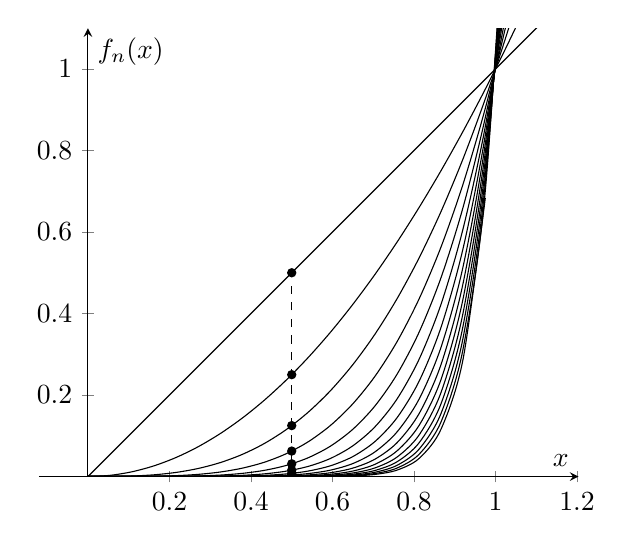
\begin{tikzpicture}
					\pgfmathsetmacro{\xzero}{.5}
					\begin{axis} [
						xlabel={$x$},ylabel={$f_n(x)$},
						axis lines=middle,
						axis equal,
						ymax = 1.1,
						legend pos = outer north east
					]
						\pgfplotsinvokeforeach{1,2,...,15} {
							% Restricting y fixes spurious lines being generated by Adobe Acrobat when printing the graph
							% Also, y domain is a bit bigger than the displayed graph since otherwise the functions wouldn't be properly plotted
							\addplot [smooth, domain=0:1.3, restrict y to domain=0:1.5] {pow(x, #1)};
							% This time around nodes are used instead of \addplot with the * mark
							% in order to control dots size, since bigger dots clutter the image
							\node[circle, fill=black, inner sep=1.2pt] at (\xzero, {pow(\xzero, #1)}) {};
						}

						\draw[dashed] (\xzero, 0) -- (\xzero, \xzero);
					\end{axis}
				\end{tikzpicture}
			}
			\caption{$x_0 = \frac{1}{2}$}
			\label{fig:conv_punt_grap_05}
		\end{subfigure}
		\begin{subfigure}{.33\textwidth}
			\centering
			\resizebox{\linewidth}{!}{
				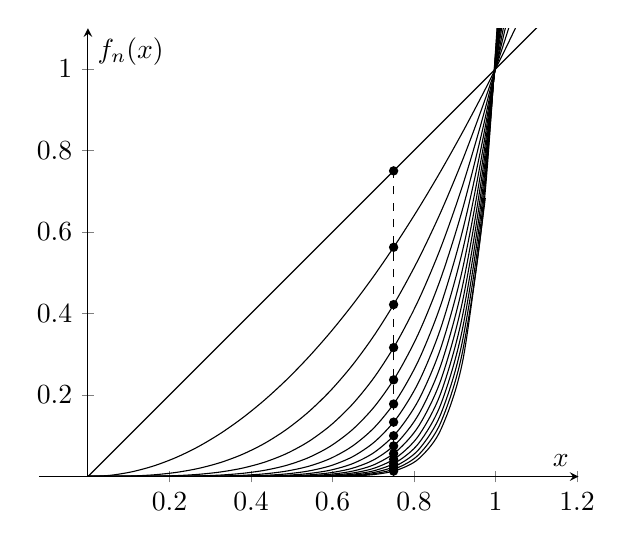
\begin{tikzpicture}
					\pgfmathsetmacro{\xzero}{.75}
					\begin{axis} [
						xlabel={$x$},ylabel={$f_n(x)$},
						axis lines=middle,
						axis equal,
						ymax = 1.1,
						legend pos = outer north east
					]
						\pgfplotsinvokeforeach{1,2,...,15} {
							% Restricting y fixes spurious lines being generated by Adobe Acrobat when printing the graph
							% Also, y domain is a bit bigger than the displayed graph since otherwise the functions wouldn't be properly plotted
							\addplot [smooth, domain=0:1.3, restrict y to domain=0:1.5] {pow(x, #1)};
							% This time around nodes are used instead of \addplot with the * mark
							% in order to control dots size, since bigger dots clutter the image
							\node[circle, fill=black, inner sep=1.2pt] at (\xzero, {pow(\xzero, #1)}) {};
						}

						\draw[dashed] (\xzero, 0) -- (\xzero, \xzero);
					\end{axis}
				\end{tikzpicture}
			}
			\caption{$x_0 = \frac{3}{4}$}
			\label{fig:conv_punt_grap_075}
		\end{subfigure}
		\begin{subfigure}{.33\textwidth}
			\centering
			\resizebox{\linewidth}{!}{
				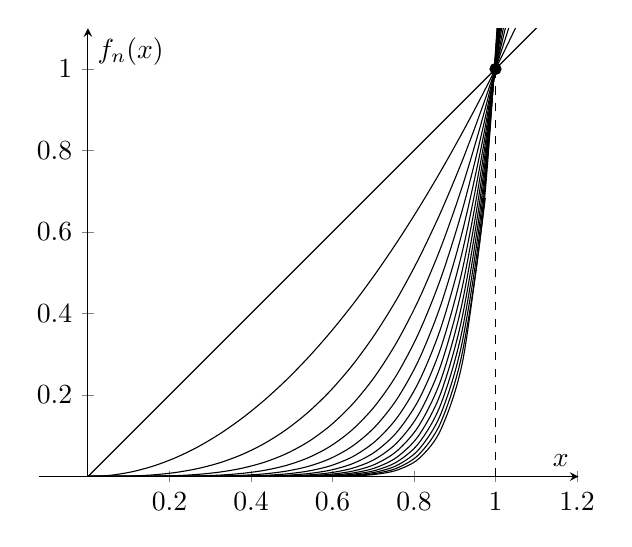
\begin{tikzpicture}
					\pgfmathsetmacro{\xzero}{1}
					\begin{axis} [
						xlabel={$x$},ylabel={$f_n(x)$},
						axis lines=middle,
						axis equal,
						ymax = 1.1,
						legend pos = outer north east
					]
						\pgfplotsinvokeforeach{1,2,...,15} {
							% Restricting y fixes spurious lines being generated by Adobe Acrobat when printing the graph
							% Also, y domain is a bit bigger than the displayed graph since otherwise the functions wouldn't be properly plotted
							\addplot [smooth, domain=0:1.3, restrict y to domain=0:1.5] {pow(x, #1)};
						}

						\addplot [color=black, only marks, mark=*] coordinates {(\xzero, \xzero)};
						\draw[dashed] (\xzero, 0) -- (\xzero, \xzero);
					\end{axis}
				\end{tikzpicture}
			}
			\caption{$x_0 = 1$}
			\label{fig:conv_punt_grap_1}
		\end{subfigure}
		\caption{Si vede che, al crescere di $n$, le $f(x_0)$ convergono a $0$ (in \ref{fig:conv_punt_grap_05} e \ref{fig:conv_punt_grap_075}) o $1$ (in \ref{fig:conv_punt_grap_1})}
	\end{figure}
\end{observation}

\begin{example}
	\label{ex:1_over_n_sin_x_punt_conv}
	La successione di Funzioni con $x \in A \equiv \R$
	\[f_n(x)=\frac{1}{n} \sin(x)\]
	è puntualmente convergente a $0$ su tutto il dominio delle $f_n$, cioè $f_n \pconvarrow 0$ su $B = A = \R$, infatti:
	\[
		\lim\limits_{n \to \infty} f_n(x) = \lim\limits_{n \to \infty} \frac{1}{n} \sin(x) = 0 \quad \forall x \in A
	\]
\end{example}
\begin{example}
	La successione
	\[f_n(x)=e^{nx}\]
	\begin{center}
		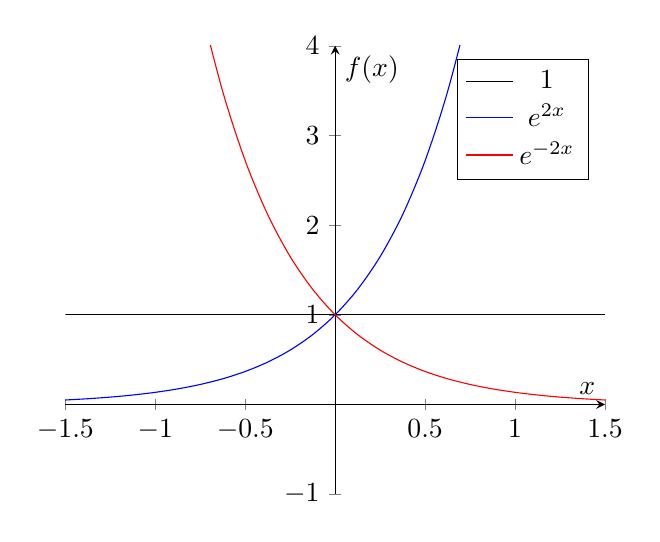
\begin{tikzpicture}
			\begin{axis}[
					xlabel={$x$},ylabel={$f(x)$},
					axis lines=middle,
					domain=-1.5:1.5,
					ymin=-1,ymax=4,
					legend pos = north east
				]
				\addplot[smooth] {1};
				\addlegendentry{$1$}
				\addplot[blue, smooth] {e^(2*x)};
				\addlegendentry{$e^{2x}$}
				\addplot[red, smooth] {e^(-2*x)};
				\addlegendentry{$e^{-2x}$}
			\end{axis}
		\end{tikzpicture}
	\end{center}
	Ha questo comportamento
	\[
		\lim\limits_{n \to \infty} e^{nx} =
		\begin{cases}
			\begin{array}{ll}
				0 & x<0\\
				1 & x=0\\
				\infty & x>0
			\end{array}
		\end{cases}
	\]
	Dunque
	\[f_n \pconvarrow f\quad \text{ su } B = \intervalopcl{-\infty}{0}\]
\end{example}

\begin{proposition}
	\label{prop:conv_punt_lim_succ}
	Siano $B \subseteq A \subseteq \R$, $\brackets{f_n:\; n \in \N}$ una \textbf{Successione di Funzioni} con $f_n:\; A \to \R$ e $f:\; B \to \R$. Allora
	\[
		f_n \pconvarrow f \text{ su } B \text{ per } n \to +\infty
		\quad \iff \quad
		\begin{cases}
			\forall \varepsilon > 0 \quad \forall x \in B\\
			\exists \nu \in \N:\; \forall n > \nu \quad \abs{f_n(x) - f(x)} \leq \varepsilon
		\end{cases}
	\]
	\begin{proof}
		Da \fullref{def:succ_punt_conv} si sa che
		\[f(x) = \lim\limits_{n \to +\infty} f_n(x) \qquad \forall x \in B\]
		Dunque, applicando la \fullref{def:lim_succ}
		\[
			\forall \varepsilon > 0 \quad \exists\nu\in\N:\; \forall n > \nu \quad d \bigl( f_n(x), f(x) \bigr) < \varepsilon  \qquad \forall x \in B
		\]
		Essendo in $f_n$ e $f$ a valori in $\R$, la $d$ è Metrica Euclidea, dunque
		\[
			\forall \varepsilon > 0 \quad \forall x \in B \quad \exists\nu\in\N:\; \forall n > \nu \quad \abs{f_n(x) - f(x)} < \varepsilon
		\]
		\vspace*{-\baselineskip}
		\begin{note}
			È possibile spostare $\forall x \in B$ "a sinistra dei $:$", in quanto, per definizione di $f$ dalla \fullref{def:succ_punt_conv}, $\forall x \in B \quad f(x) = \lim$, quindi la relazione è sempre valida, a prescindere dalla scelta di $x$.
		\end{note}
	\end{proof}
\end{proposition}
\begin{proposition}
	Siano $B \subseteq A \subseteq \R$, $\brackets{f_n:\; n \in \N}$ una \textbf{Successione di Funzioni} con $f_n:\; A \to \R$ e $F:\; B \to \R$. Allora
	\[
		\sum\limits_{n = 0}^{+\infty} f_n \pconvarrow F \text{ su } B
		\quad \iff \quad
		\begin{cases}
			\forall \varepsilon > 0 \quad \forall x \in B\\
			\exists \nu \in \N:\; \forall n > \nu \quad \abs{\sum\limits_{n = 0}^{k} f_n(x) - F(x)} \leq \varepsilon
		\end{cases}
	\]
	\begin{proof}
		Analoga alla \fullref{prop:conv_punt_lim_succ} ricordando la definizione di $F$ in \fullref{def:serie}.
	\end{proof}
\end{proposition}

\begin{proposition}[Metaproposizione sulle Proprietà delle Successioni]
	Sia $f_n:\; A \to \R$, $B \subseteq A \subseteq \R$, $f:\; B \to \R$\\
	Se $f_n \pconvarrow f$ su $B$ e se $f_n$ ha la proprietà $P$, allora la funzione limite puntuale $f$ ha a sua volta la proprietà $P$.
	\begin{note}
		La continuità (e quindi anche la derivabilità) non è una proprietà che passa alla funzione limite, come visto in \fullref{ex:conv_succ_xn}, dove la $f$ ha un punto di discontinuità in $x = 1$.
	\end{note}
	\begin{proof}
		Verrà svolta per le singole proprietà.
	\end{proof}
\end{proposition}
\begin{exercise}
	\label{ex:dim_prop_lim_conv_punt}
	Enunciare rigorosamente e dimostrare:
	\begin{enumerate}
		\item Il limite puntuale della somma (prodotto, combinazione lineare) di due successioni di funzioni è la somma (prodotto, combinazione lineare) delle funzioni limiti puntuali
		\item \label{itm:prop_lim_punt_non_neg} Il limite puntuale di una successione di funzioni non negative è una funzione non negativa
		\item \label{itm:prop_lim_punt_monotonia} Il limite puntuale di una successione di funzioni debolmente/strettamente crescenti/decrescenti è una funzione debolmente crescente/decrescente
		\item Il Criterio di Cauchy (da \fullref{def:succ_cau}) per la convergenza puntuale di serie e successioni
		\item Se la serie $\sum\limits_{n = 0}^{+\infty} f_n(x)$ converge puntualmente in un insieme $B$, allora $f_n \pconvarrow 0$ su $B$
	\end{enumerate}
	\begin{solution}~
		\renewcommand\qedsymbol{$\square$} % To restore the default empty square for the proof environments below
		\begin{enumerate}
			\item[\ref{itm:prop_lim_punt_non_neg}.]
				Sia $f_n:\; A \to \R$, $B \subseteq A \subseteq \R$ e $f:\; B \to A$\\
				Se $f_n \pconvarrow f$ su $B$ e se $f_n$ è non negativa su $B$, cioè $f_n \geq 0$, allora il limite puntuale $f$ è non negativo, $f \geq 0$, su $B$.
				\begin{proof}
					Da \fullref{def:succ_punt_conv}, si sa che
					\[f(x) = \lim\limits_{n \to \infty} f_n(x) \quad \forall x \in B\]
					Ma $f_n$ è, per ipotesi, una successione di valori non negativi, quindi il limite esiste ed è non negativo.

					La dimostrazione è analoga per funzioni non positive.
				\end{proof}
			\item[\ref{itm:prop_lim_punt_monotonia}.]
				Sia $f_n:\; A \to \R$, $B \subseteq A \subseteq \R$ e $f:\; B \to A$\\
				Se $f_n \pconvarrow f$ su $B$ e se $f_n$ è debolmente crescente su $B$, allora il limite puntuale $f$ è debolmente crescente su $B$.
				\begin{proof}
					Il fatto che $f_n$ sia debolmente crescente su $B$ implica che
					\[\forall x_1, x_2 \in B \quad x_1 \leq x_2 \implies f_n(x_1) \leq f_n(x_2)\]
					Con $n \to \infty$, essendo nell'insieme $B$, si ha che $f(x_1) \leq f(x_2)$ per definizione di $f$ da \fullref{def:succ_punt_conv}.

					La dimostrazione è analoga per funzioni debolmente decrescenti e strettamente/debolmente crescenti.
					\let\qed\relax % In order to avoid having two squares, hide the innermost one
				\end{proof}
			% TODO remaining points
			\vspace*{-2\baselineskip} % To remove the whitespace due to enumerate environment
		\end{enumerate}
	\end{solution}
\end{exercise}
\begin{observation}
	In riferimento al punto \ref{itm:prop_lim_punt_non_neg} dell'\fullref{ex:dim_prop_lim_conv_punt}, è necessario sottolineare come non sia invece possibile avere certezze sulla \textbf{stretta} positività/negatività del limite puntuale di una successione di funzioni strettamente positive/negative.\\
	Ad esempio, $-\frac{e^x}{n}$ con $x \in \intervalclop{0}{1}$ è strettamente negativa, ma il limite puntuale è costante $0$.
\end{observation}
\begin{observation}
	In riferimento al punto \ref{itm:prop_lim_punt_monotonia} dell'\fullref{ex:dim_prop_lim_conv_punt}, è necessario sottolineare come non sia invece possibile avere certezze sulla \textbf{stretta} crescenza/decrescenza del limite puntuale.\\
	Come esempio, vedasi \fullref{ex:conv_succ_xn} in cui si studia la successione strettamente crescente $x^n$, il cui limite puntuale è però costante (dunque non \textbf{strettamente} crescente) in $B = \intervalclop{0}{1}$.
\end{observation}
\begin{exercise}
	Verificare che il limite puntuale di funzioni \textbf{Continue} e \textbf{Derivabili}, quando esiste, può essere una funzione \textbf{Continua} e \textbf{non Derivabile}.\\
	Considerare ad esempio $f_n:\; \R \to \R$ data da $f_n(x) = \sqrt{x^2 + \frac{1}{n}}$ visibile in \cref{fig:fn_sqrt_x2_1_over_n}.
	% TODO solution
\end{exercise}
\begin{exercise}
	Verificare che il limite puntuale di funzioni \textbf{Continue} e \textbf{Derivabili}, quando esiste, può essere una funzione \textbf{non Continua}.\\
	Considerare ad esempio $f_n:\; \R \to \R$ data da $f_n(x) = \arctan(nx)$ visibile in \cref{fig:fn_sqrt_x2_1_over_n}.
	% TODO solution
\end{exercise}
\begin{exercise}
	Determinare, se possibile, sotto quali ipotesi sulla funzione $f:\; \R \to \R$ le seguenti successioni di funzioni risultano Puntualmente Convergenti:
	\begin{align*}
		f_n(x) &= f(x) + n & f_n(x) &= f(x + n)\\
		f_n(x) &= f(x) + \frac{1}{n} & f_n(x) &= f(x + \frac{1}{n})\\
		f_n(x) &= nf(x) & f_n(x) &= \frac{f(x)}{n}\\
		f_n(x) &= f(nx) & f_n(x) &= f(\frac{x}{n})
	\end{align*}
\end{exercise}

\cbstart
\begingroup
% This group is used to alter equation numbering, since there are equations outside environments
\renewcommand\theequation{\arabic{section}.\arabic{equation}}
\setcounter{equation}{0} % Reset counter to fix numbering for equation outside theorem envs
\subsection{L'Insufficienza della Convergenza Puntuale}\label{sect:insuff_conv_punt}
La Convergenza Puntuale si può rivelare insufficiente per diverse ragioni, tra cui:
\begin{itemize}
	\item
		Può spesso esser comodo utilizzare una successione $f_n$ convergente puntualmente a $f$ nel caso in cui $f$ non sia ottenibile in modo esplicito (ad esempio nella soluzione di un'equazione differenziale). Però, come visto in \fullref{ex:conv_succ_xn}, la convergenza puntuale non trasferisce necessariamente proprietà come Continuità, Limitatezza o Derivabilità alla funzione limite puntuale.
		La successione $f_n = x^n$ di \fullref{ex:conv_succ_xn}, ad esempio, è formata da funzioni $\in \cntclass{\infty}(\intervalclose{0}{1}; \R)$, però la funzione limite puntuale
		\[
			f =
			\begin{cases}
				\begin{array}{ll}
					0 & \text{se } x \in \intervalopen{-1}{1}\\
					1 & \text{se } x = 1
				\end{array}
			\end{cases}
		\]
		non è né continua né, dunque, derivabile nello stesso intervallo.
		\begin{figure}[H]
			\begin{subfigure}{.49\textwidth}
				\centering
				\resizebox{\linewidth}{!}{
					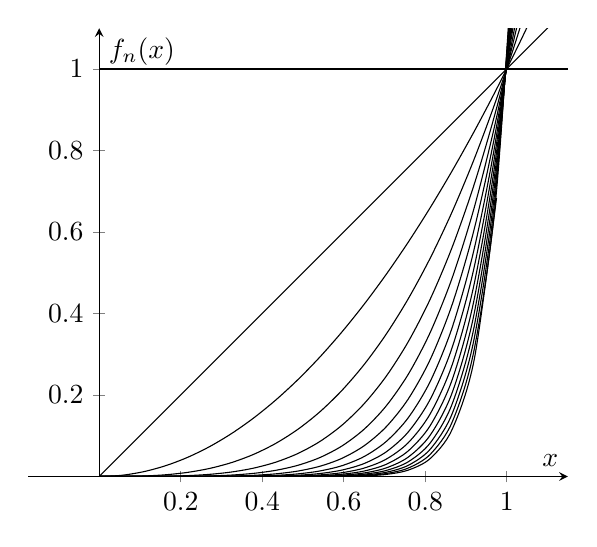
\begin{tikzpicture}
						\begin{axis} [
							xlabel={$x$},ylabel={$f_n(x)$},
							axis lines=middle,
							axis equal,
							% xmax is used only to force same width to both graphs, thus having same height when resized
							ymax = 1.1, xmax = 1.15,
							legend pos = outer north east
						]
							\pgfplotsinvokeforeach{0,1,...,15} {
								% Restricting y fixes spurious lines being generated by Adobe Acrobat when printing the graph
								% Also, y domain is a bit bigger than the displayed graph since otherwise the functions wouldn't be properly plotted
								\addplot [smooth, domain=0:1.3, restrict y to domain=0:1.5] {pow(x, #1)};
							}
						\end{axis}
					\end{tikzpicture}
				}
				\caption{$f_n(x) = x^n \quad 0 \leq n \leq 15$}
			\end{subfigure}
			\begin{subfigure}{.49\textwidth}
				\centering
				\resizebox{\linewidth}{!}{
					\begin{tikzpicture}
						\begin{axis} [
							xlabel={$x$},ylabel={$f(x)$},
							axis lines=middle,
							axis equal,
							% xmax is used only to force same width to both graphs, thus having same height when resized
							ymax = 1.1, xmax = 1.15,
							legend pos = outer north east
						]
							\addplot [smooth, line width=2pt, domain=0:1] {0};
							\addplot [color=black, fill=white, only marks, mark=*] coordinates {(1,0)};
							\addplot [color=black, only marks, mark=*] coordinates {(1,1)};
						\end{axis}
					\end{tikzpicture}
				}
				\caption{$f(x) \quad x \in \intervalclose{0}{1}$}
			\end{subfigure}
			\caption{$f_n(x) \in \cntclass{\infty}(\intervalclose{0}{1}; \R)$, mentre la funzione limite puntuale $f$ è discontinua.}
			\label{fig:cont_fn_non_passa_a_f}
		\end{figure}
	\item
		Supponendo di voler calcolare l'integrale
		\begin{equation}
			\label{eq:insuf_conv_punt_int_f}
			\int_a^b f(x) \integrald{x}
		\end{equation}
		Ma con $f$ non integrabile (o magari anche solo $f$ non integrabile in modo elementare). Si cercherebbe dunque di approssimarlo con una successione di integrali tipo
		\begin{equation}
			\label{eq:insuf_conv_punt_int_fn}
			\int_a^b f_n(x) \integrald{x}
		\end{equation}
		Potrebbe venire naturale di prendere una successione $f_n$ Puntualmente Convergente a $f$ e quindi considerare gli integrali delle $f_n$ della \cref{eq:insuf_conv_punt_int_fn} come approssimazioni dell'integrale \cref{eq:insuf_conv_punt_int_f}. Questo ragionamento è però valido solo nel caso in cui valga
		\begin{equation}
			\label{eq:conv_punt_pass_lim_integrale}
			\lim\limits_{n \to +\infty} \int_a^b f_n(x) \integrald{x} = \int_a^b \lim\limits_{n \to +\infty} f_n(x) \integrald{x} = \int_a^b f(x) \integrald{x}
		\end{equation}
		Cioè eseguendo il \textit{passaggio al limite sotto il segno di integrale}, operazione di cui si è già parlato nell'introduzione al \fullref{chap:int_doppi} specificando che, con gli integrali di Riemann, non è affatto scontato sia possibile.\\
		Nel caso della convergenza puntuale non son garantite le ipotesi necessarie, dunque non è possibile passare al limite sotto l'integrale, come si vede nel successivo \fullref{ex:conv_punt_no_pass_lim_integrale}.
\end{itemize}
La Convergenza Puntuale presenta le problematiche evidenziate in quanto non si basa su alcun tipo di concetto di \textbf{distanza tra funzioni}. Infatti, ricordando \fullref{def:succ_punt_conv}, avere convergenza puntuale $f_n \pconvarrow f$ su un certo insieme $A$ significa che, fissato un qualsiasi $x_0 \in A$, si ha
\[\lim\limits_{n \to +\infty} d \bigl( f_n(x_0), f(x_0) \bigr) = 0\]
Con $d$ Metrica Euclidea, distanza tra i valori di $f_n$ ed $f$ nel punto $x_0$ precedentemente fissato. In pratica, i valori di $f_n$ e $f$ vengono considerati \textbf{punto per punto} separatamente e la convergenza puntuale non è influenzata da tutti gli altri valori che le funzioni possono assumere in un intorno di $x_0$.
\begin{example}
	\label{ex:conv_punt_no_pass_lim_integrale}
	La successione
	\[
		\funcdef{f_n}{\intervalclose{0}{1}}{\R}{x}{
			\begin{cases}
				\begin{array}{ll}
					0 & \text{se } x \in \brackets{0} \cup \intervalopcl{\frac{1}{n}}{1}\\
					-n^2x + n & \text{se } x \in \intervalopcl{0}{\frac{1}{n}}
				\end{array}
			\end{cases}
		}
	\]
	converge puntualmente alla funzione $f(x) = 0$ su $\intervalclose{0}{1}$. Infatti, essendo $\frac{1}{n} \to 0$ per $n \to +\infty$, un qualsiasi $x \in \intervalclose{0}{1}$ cadrà nell'intervallo $\intervalopcl{\frac{1}{n}}{1}$ in cui $f_n$ è definita essere $0$. Quindi $\lim\limits_{n \to +\infty} f_n(x) = 0$.
	\begin{center}
		\begin{tikzpicture}
			\begin{axis} [
				clip mode = individual,
				xlabel={$x$},ylabel={$f_n(x)$},
				axis lines=middle,
				xmax=1.2, ymax=5.5,
				xtick = {1/2, 1},
				xticklabels = {$\frac{1}{n}$, $1$},
				ytick = {2},
				yticklabels = {$n$}
			]
				\addplot [color=black, only marks, mark=*] coordinates {(0,0)};
				\pgfplotsinvokeforeach{2, 3, 5} {
					\addplot [thick, domain=0:(1/#1)] {-pow(#1, 2)*x + #1};
					\addplot [color=black, fill=white, only marks, mark=*] coordinates {(0,#1)};
				}
				\addplot [line width=2pt, domain=(1/5):1] {0}; % We need only a single line on x axis, the one starting at the smallest 1/n
			\end{axis}
		\end{tikzpicture}
	\end{center}
	Gli integrali delle $f_n$ sono:
	\begin{align*}
		&\int_0^1 f_n(x) \integrald{x} =\\
		&= \int_0^{\frac{1}{n}} \left( -n^2x + n \right)\integrald{x} + \int_{\frac{1}{n}}^1 0 \integrald{x}\\
		&= \left[ -\frac{n^2}{2}x^2 + nx \right]_0^{\frac{1}{n}}\\
		&= -\frac{n^2}{2}\frac{1}{n^2} + n \frac{1}{n}\\
		&= \frac{1}{2}
	\end{align*}
	L'integrale della funzione limite puntuale $f$ sarebbe, ovviamente, $0$, essendo stato dimostrato prima che $f_n \pconvarrow 0$, dunque l'uguaglianza di \cref{eq:conv_punt_pass_lim_integrale} non vale.
\end{example}

\subsection{Distanze tra Funzioni}\label{sect:dist_funz}
La nozione di distanza si basa, generalmente, su una preesistente nozione di "grandezza": stabilito il modo per valutare la grandezza di un ente, è ragionevole ritenere che due oggetti siano tanto più vicini quanto più è "piccola" la differenza tra essi. Cioè la distanza può essere vista come la "grandezza" della differenza (ovviamente, quando è ammessa la differenza tra gli oggetti). Si è vista l'applicazione di questo criterio in molti esempi di \fullref{ex:metriche}.

Dovendo valutare la distanza tra funzioni, è dunque necessario prima stabilire come valutare la "grandezza" delle funzioni stesse.

Quale delle seguenti funzioni ha senso definire "più grande"?
\begin{figure}[H]
	\begin{subfigure}{.49\textwidth}
		\centering
		\resizebox{\linewidth}{!}{
			\begin{tikzpicture}
				\begin{axis} [
					xlabel={$x$},ylabel={$f(x)$},
					axis lines=center,
					axis on top = true,
					axis equal,
					xmin = -4, xmax = 4,
					ymin = -.5, ymax = 6,
					xtick = {-3, 3},
					xticklabels = {$a$, $b$}
				]
					\addplot [name path=f, smooth, domain=-5:5, samples=50] {exp(-10*x^2)*5};
					\path[name path=axis] (\pgfkeysvalueof{/pgfplots/xmin},0) -- (\pgfkeysvalueof{/pgfplots/xmax},0);
					\addplot[black!30] fill between[of=f and axis, soft clip={domain=-3:3}];
				\end{axis}
			\end{tikzpicture}
		}
		\caption{Curva gaussiana}
		\label{pic:grand_funz_gauss}
	\end{subfigure}
	\begin{subfigure}{.49\textwidth}
		\centering
		\resizebox{\linewidth}{!}{
			\begin{tikzpicture}
				\begin{axis} [
					xlabel = $x$, ylabel = {$f(x)$},
					axis lines = center,
					axis on top = true,
					axis equal,
					xmin = -4, xmax = 4,
					ymin = -.5, ymax = 6,
					xtick = {-3, 3},
					xticklabels = {$a$, $b$}
				]
					\addplot [name path=f, smooth, domain=-5:5, samples=50] {-(4/7*x)^2+3};
					\path[name path=axis] (\pgfkeysvalueof{/pgfplots/xmin},0) -- (\pgfkeysvalueof{/pgfplots/xmax},0);
					\addplot[black!30] fill between[of=f and axis, soft clip={domain=-3:3}];
				\end{axis}
			\end{tikzpicture}
		}
		\caption{Parabola rovesciata}
		\label{pic:grand_funz_parab}
	\end{subfigure}
	\caption{Diversi parametri per valutare la "grandezza" di una funzione}
\end{figure}

Ovviamente dipende dall'aspetto che si intende considerare. La \ref{pic:grand_funz_gauss} potrebbe essere "più grande" perché ha massimo maggiore rispetto a \ref{pic:grand_funz_parab}, che però d'altro canto ha una maggiore area sottesa.

Questi erano solo due esempi di "grandezza" di una funzione, definiti con le seguenti metriche
\[
	\norm{f}_{\cntclass{0}} = \sup\limits_{x \in \intervalclose{a}{b}} \abs{f(x)}
	\qquad\qquad\qquad\qquad\qquad
	\norm{f}_1 = \int_a^b \abs{f(x)} \integrald{x}
\]
Quella di sinistra è la \textbf{Norma Infinito} o \textbf{Norma del} $\boldsymbol{\sup}$, mentre a destra \textbf{Norma Indice} $\boldsymbol{1}$. In aggiunta, si definisce anche la \textbf{Norma Indice} $\boldsymbol{2}$, che sarà usata in \fullref{sect:conv_quadr}:
\index{Norma!Infinito}
\index{Norma!Indice 1}
\index{Norma!Indice 2}
\[\norm{f}_2 = \sqrt{ \int_a^b \left[f(x)\right]^2 \integrald{x} }\]

Le distanze indotte dalle seguenti norme saranno dunque
\index{Distanza!Infinito}\index{Metrica!Infinito}
\index{Distanza!Indice 1}\index{Metrica!Indice 1}
\index{Distanza!Indice 2}\index{Metrica!Indice 2}
\[
	d_{\cntclass{0}} (f, g) = \norm{f - g}_{\cntclass{0}}
	\qquad\qquad\qquad
	d_1 = \norm{f - g}_1
	\qquad\qquad\qquad
	d_2 = \norm{f - g}_2
\]
E si parla di \textbf{Distanza Infinito} (o \textbf{Distanza del} $\boldsymbol{\sup}$), \textbf{Distanza Indice} $\boldsymbol{1}$ e \textbf{Distanza Indice} $\boldsymbol{2}$.

\begin{figure}[H]
	\begin{subfigure}{.49\textwidth}
		\centering
		\resizebox{\linewidth}{!}{
			\begin{tikzpicture}[
				declare function = {
					f(\x) = sqrt(\x)*(sin(deg(\x))+1);
					g(\x) = sqrt(\x);
				},
				> = stealth
			]
			\begin{axis} [
				xlabel={$x$},ylabel={$y$},
				axis lines=middle,
				ymax=9,
				legend style = {at={(.1,.95)}, anchor = north west}
			]
				\addplot [thick, name path=f, smooth, domain=0:10, samples=50] {f(x)};
				\addlegendentry{$f$};
				\addplot [color=blue!60, thick, name path=g, smooth, domain=0:10, samples=100] {g(x)};
				\addlegendentry{$g$};
				\pgfplotsinvokeforeach{.25,.5,...,10} {
					\draw[thin, black!60] (#1, {f(#1)}) -- (#1, {g(#1)});
				}
				% Mark thicker the sup
				\draw[thick] (8, {g(8)}) -- (8,{f(8)});
				\node (text_sup_dist) [align=center] at (6.5,8) {$\sup \abs{f(x) - g(x)}$};
				\draw[thin, ->, shorten >=4pt] (text_sup_dist.south) to [out=-90, in=90](8,{f(8)});

				\addplot[brown!30] fill between[of=f and g];
				\addlegendentry{$d_1$};
			\end{axis}
		\end{tikzpicture}
		}
		\caption{Significato grafico di\\Distanza Infinito e Distanza Indice $1$}
	\end{subfigure}
	\begin{subfigure}{.49\textwidth}
		\centering
		\resizebox{\linewidth}{!}{
			\begin{tikzpicture}[
				declare function = {
					f(\x) = sqrt(\x)*(sin(deg(\x))+1);
					g(\x) = sqrt(\x);
				},
				> = stealth
			]
				\begin{axis} [
					xlabel={$x$},ylabel={$y$},
					axis lines=middle,
					axis on top = true,
					ymax=9,
					legend style = {at={(.1,.95)}, anchor = north west}
				]
					\addplot [thick, name path=f, smooth, domain=0:10, samples=100] {(f(x)-g(x))^2};
					\addlegendentry{$\bigl[ f(x) - g(x) \bigr]^2$};
					\path[name path=axis] (\pgfkeysvalueof{/pgfplots/xmin},0) -- (\pgfkeysvalueof{/pgfplots/xmax},0);
					\addplot[brown!30] fill between[of=f and axis];
					\addlegendentry{$d_2$};
				\end{axis}
			\end{tikzpicture}
		}
		\caption{Significato grafico (a meno della radice) di\\Distanza Indice $2$}
	\end{subfigure}
\end{figure}
\cbend
\endgroup

\subsection{Convergenza Uniforme}\label{sect:conv_unif}\index{Convergenza!Uniforme}
Si chiama Convergenza Uniforme la convergenza di una Successione di Funzioni rispetto alla distanza $d_{\cntclass{0}}$.

\begin{definition}[Successione Uniformemente Convergente]
	\index{Successione!Convergente Uniformemente}
	\label{def:succ_unif_conv}
	Siano $B \subseteq A \subseteq \R$, $\brackets{f_n:\; n \in \N}$ una \textbf{Successione di Funzioni} e $f_n:\; A \to \R$.\\
	La Successione $f_n$ è \textbf{Uniformemente Convergente} su $B$ se esiste la \textbf{Funzione Limite Uniforme} $f:\; B \to \R$ tale che:
	\[\lim\limits_{n \to +\infty} \sup\limits_{B} \abs{f_n(x) - f(x)} = 0\]
	\begin{note}
		Nella \fullref{def:succ_punt_conv} la $f$ associava ogni punto al valore a cui convergeva la successione in quel punto.\\
		In questo caso invece la $f$ è una funzione \textit{tale per cui} la distanza massima (per via del $\sup$ di $d_{\cntclass{0}}$) tra $f_n$ e $f$ è $0$. Questo vuol dire che la funzione "coincide con la $f_n$ su tutto $B$", in quel senso \textit{Uniformemente}. Vedasi \fullref{obs:diff_conv_unif_e_conv_punt}.
	\end{note}
	La convergenza uniforme su $B$ della successione $f_n$ verso $f$ è indicata con
	\[f_n \uconvarrow f \text{ su } B\]
\end{definition}
\begin{definition}[Serie Uniformemente Convergente]
	\index{Serie!Uniformemente Convergente}
	Siano $B \subseteq A \subseteq \R$, $\brackets{f_n:\; n \in \N}$ una \textbf{Successione di Funzioni} e $f_n:\; A \to \R$.\\
	La \textbf{Serie} $s = \sum\limits_{n = 0}^{+\infty} f_n(x)$ associata alla Successione $f_n$ è \textbf{Uniformemente Convergente} su $B$ se esiste la \textbf{Funzione Limite Uniforme} $F:\; B \to \R$ tale che:
	\[\lim\limits_{n \to +\infty} \sup\limits_{B} \abs{\sum\limits_{n = 0}^{+\infty} f_n(x) - F(x)} = 0\]
\end{definition}

\newpage % WARNING Check this is not generating too much whitespace
\begin{example}~
	\begin{figure}[H]
		\centering
		\begin{tikzpicture}[
			declare function = {
				f_n(\x) = sqrt(\x)*(1/4*(sin(deg(\x))+4));
				f(\x) = sqrt(\x);
			},
			> = stealth
		]
			\begin{axis} [
				xlabel={$x$},ylabel={$y$},
				axis lines=middle,
				axis on top = true,
				ymax=9,
				legend style = {at={(.1,.95)}, anchor = north west}
			]
				\addplot [thick, name path=f_n, smooth, domain=0:10, samples=50] {f_n(x)};
				\addlegendentry{$f_n$};
				\addplot [color=blue!60, thick, smooth, domain=0:10, samples=100] {f(x)};
				\addlegendentry{$f$};
				\addplot [color=red, name path=f_plus, smooth, domain=0:10, samples=100] {f(x) + 1.2};
				\addlegendentry{$f + \varepsilon$};
				\addplot [color=green, name path=f_minus, smooth, domain=0:10, samples=100] {f(x) - 1.2};
				\addlegendentry{$f - \varepsilon$};
				\pgfplotsinvokeforeach{.25,.5,...,10} {
					\draw[thin, black!60] (#1, {f_n(#1)}) -- (#1, {f(#1)});
				}
				% Mark thicker the sup
				\draw[thick] (8, {f(8)}) -- (8,{f_n(8)});
				\node (text_sup_dist) [align=center] at (7,6.5) {$\sup \abs{f_n(x) - f(x)} < \varepsilon$};
				\draw[thin, ->, shorten >=2pt] (text_sup_dist.south) to [out=-90, in=90](8,{f_n(8)});

				\addplot[brown!30, forget plot] fill between[of=f_plus and f_minus];
			\end{axis}
		\end{tikzpicture}
		\caption{Significato grafico della Convergenza Uniforme\\Come si vedrà in {\protect\fullref{prop:conv_unif_lim_succ}}}
	\end{figure}
\end{example}

\begin{observation}
	\label{obs:dist_conv_unif}
	La convergenza uniforme equivale alla convergenza rispetto alla distanza $d_{\cntclass{0}}(f,g)=\sup\limits_{x\in A}\abs{g(x)-f(x)}$ ogniqualvolta questa distanza sia definita. La definizione di $d_{\cntclass{0}}(f,g)$ come \textit{distanza} è dimostrata in \hyperref[ex:dim_dist_conv_unif]{\fullref*{ex:metriche}}\\
	% NOTE The \fullref command was not used on purpose to point this link straight to the right part of the aforementioned exercise
	La $d_{\cntclass{0}}(f,g)$ può anche essere definita attraverso la \textbf{norma} $\norm{k}_{\cntclass{0}}=\sup\limits_{x\in A}\abs{k}$ con $k = f-g$ in quanto, in $\R$ norma e valore assoluto coincidono.
\end{observation}
\begin{example}
	Come già visto in \fullref{ex:1_over_n_sin_x_punt_conv}, la Successione di Funzioni con $x \in A \equiv \R$
	\[f_n(x) = \frac{1}{n} \sin(x)\]
	è $f_n \pconvarrow 0$ su $A$. Questa stessa Successione è anche Uniformemente Convergente su $A$, infatti:
	\[
		\lim\limits_{n \to +\infty} \sup\limits_{A} \abs{f_n(x) - 0} =
		\lim\limits_{n \to +\infty} \sup\limits_{A} \abs{\frac{1}{n} \sin(x)}
	\]
	Osservando che $\abs{a \cdot \sin(x)} \leq \abs{a}$, si può concludere
	\[
		\lim\limits_{n \to +\infty} \sup\limits_{\R} \abs{\frac{1}{n} \sin(x)} \leq
		\lim\limits_{n \to +\infty} \frac{1}{n}=0
	\]
	Allora $f_n \uconvarrow f$ su $A$
\end{example}

\begin{exercise}
	\label{ex:dim_dist_inf}
	Sia $K \in \R$ un \textbf{Compatto}. Verificare che:
	\begin{enumerate}
		\item $\norm{\;\cdot\;}_{\cntclass{0}}$ è una norma su $\cntclass{0}(K; \R)$
		\item \label{itm:dim_dist_inf_dist} $d_{\cntclass{0}}$ è una distanza su $\cntclass{0}(K; \R)$
		\item La convergenza rispetto alla distanza $d_{\cntclass{0}}$ equivale alla convergenza uniforme su $K$
	\end{enumerate}
	\begin{solution}~
		\begin{enumerate}
			\item[\ref{itm:dim_dist_inf_dist}.] Dimostrata in \hyperref[ex:dim_dist_conv_unif]{\fullref*{ex:metriche}}
			% NOTE The \fullref command was not used on purpose to point this link straight to the right part of the aforementioned exercise
		\end{enumerate}
		% TODO remaining points proof
	\end{solution}
\end{exercise}
\begin{proposition}
	\label{prop:conv_unif_lim_succ}
	Siano $B \subseteq A \subseteq \R$, $\brackets{f_n:\; n \in \N}$ una \textbf{Successione di Funzioni} e $f_n:\; A \to \R$. Sia $f:\; B \to \R$ una funzione:
	\[
		f_n \uconvarrow f \text{ su } B \text{ per } n \to +\infty
		\quad \iff \quad
		\begin{cases}
			\forall \varepsilon > 0 \quad \exists \nu \in \N:\\
			\forall n > \nu \quad \forall x \in B \quad \abs{f_n(x) - f(x)} \leq \varepsilon
		\end{cases}
	\]
	\begin{solution}
		Da \fullref{def:succ_unif_conv} si sa che
		\[\lim\limits_{n \to +\infty} \sup\limits_{B} \abs{f_n(x) - f(x)} = 0\]
		Dunque, applicando la \fullref{def:lim_succ}
		\[
			\forall \varepsilon > 0 \quad \exists\nu\in\N:\; \forall n > \nu \quad d \bigl( \abs{f_n(x) - f(x)}, 0 \bigr) < \varepsilon  \qquad \forall x \in B
		\]
		Essendo in $f_n$ e $f$ a valori in $\R$, la $d$ è Metrica Euclidea, dunque
		\[
			\forall \varepsilon > 0 \quad \exists\nu\in\N:\; \forall n > \nu \quad \forall x \in B \quad \bigl| \abs{f_n(x) - f(x)} - 0 \bigr| < \varepsilon
		\]
		\begin{note}
			A differenza di quanto fatto in \fullref{prop:conv_punt_lim_succ}, non è possibile spostare $\forall x \in B$ "a sinistra dei $:$". La scelta di $x$ non è \textit{"a prescindere"}, ma subordinata alla scelta di $\varepsilon$ e $\nu$. Dato dunque un certo $\nu$, allora, per ogni $n$ e $x$, vale il limite. Vedasi \fullref{obs:diff_conv_unif_e_conv_punt}.
		\end{note}
	\end{solution}
\end{proposition}
\begin{proposition}
	Siano $B \subseteq A \subseteq \R$, $\brackets{f_n:\; n \in \N}$ una \textbf{Successione di Funzioni} con $f_n:\; A \to \R$ e $F:\; B \to \R$. Allora
	\[
		\sum\limits_{n = 0}^{+\infty} f_n \uconvarrow F \text{ su } B
		\quad \iff \quad
		\begin{cases}
			\forall \varepsilon > 0 \quad \exists \nu \in \N:\\
			\forall n > \nu \quad \forall x \in B \quad \abs{\sum\limits_{n = 0}^{k} f_n(x) - F(x)} \leq \varepsilon
		\end{cases}
	\]
	\begin{proof}
		Analoga alla \fullref{prop:conv_unif_lim_succ} ricordando la definizione di $F$ in \fullref{def:serie}.
	\end{proof}
\end{proposition}
\begin{observation}
	\label{obs:diff_conv_unif_e_conv_punt}
	La differenza tra \fullref{prop:conv_unif_lim_succ} e \fullref{prop:conv_punt_lim_succ} (e rispettive proposizioni sulle Serie) giustifica il fatto che la continuità non passi alla Funzione Limite Puntuale, come spiegato in \fullref{sect:insuff_conv_punt}.

	Infatti qui $\nu$ dipende solo dalla scelta di $\varepsilon$ e le $x$ "si guardano tutte insieme", nella Convergenza Puntuale invece $\nu$ dipendeva, oltre che dalla $\varepsilon$, anche dalla $x$. Questo portava ad osservare le $x$ una alla volta.
\end{observation}
\begin{corollary}[Relazione tra Convergenza Uniforme e Puntuale]
	\label{coro:if_unif_conv_then_punt_conv}
	Siano $B \subseteq A \subseteq \R$ e $\brackets{f_n:\; n \in \N}$ una \textbf{Successione di Funzioni} e $f_n:\; A \to \R$. Sia $f:\; B \to \R$ una funzione
	\[f_n \uconvarrow f \text{ su } B \quad \implies \quad  f_n \pconvarrow f \text{ su } B\]
	\vspace*{-\baselineskip}
	\begin{note}
		Questo significa che la Convergenza Uniforme ha tutte le proprietà della Convergenza Puntuale.
	\end{note}
	\begin{note}
		L'implicazione inversa non è possibile, come si vede in \fullref{ex:conv_punt_nimplies_conv_unif}.
	\end{note}
	\begin{proof}
		Da \fullref{prop:conv_unif_lim_succ}  si sa che valgono condizioni analoghe, ma più restrittive, rispetto a quelle di \fullref{prop:conv_punt_lim_succ} (vedere note alle due Proposizioni), dunque sicuramente è valida l'implicazione $\impliedby$ di \fullref{prop:conv_punt_lim_succ}.
	\end{proof}
\end{corollary}
\begin{example}[La Convergenza Puntuale non implica Convergenza Uniforme]
	\label{ex:conv_punt_nimplies_conv_unif}
	Sia $f_n:\; \R \to \R$ data da $f_n(x) = x^n$, allora:
	\[
		f_n \pconvarrow f \text{ su } \intervalopcl{-1}{1}
		\qquad \text{dove} \qquad
		f(x) = \begin{cases}
			\begin{array}{ll}
				0 & \text{per } x \in \intervalopen{-1}{1}\\
				1 & \text{per } x = 1
			\end{array}
		\end{cases}
	\]
	Ma su $\intervalopcl{-1}{1}$ non c'è convergenza uniforme e nemmeno su $\intervalopen{-1}{1}$.
\end{example}
\begin{exercise}
	È possibile costruire una successione di funzioni $f_n$ uniformemente convergenti ad una successione $f$ non limitata?
	\begin{solution}
		No, perché, come visto in \fullref{coro:if_unif_conv_then_punt_conv} $f_n \uconvarrow f \implies f_n \pconvarrow f$, ma per \fullref{def:succ_punt_conv} $\nexists$ successione puntualmente convergente a $f$ non limitata.
		% TODO controllare soluzione
	\end{solution}
\end{exercise}
\begin{exercise}
	Determinare, se possibile, sotto quali ipotesi sulla funzione $f:\; \R \to \R$ le seguenti successioni di funzioni sono Uniformemente Convergenti:
	\begin{align*}
		f_n(x) &= f(x) + n & f_n(x) &= f(x + n)\\
		f_n(x) &= f(x) + \frac{1}{n} & f_n(x) &= f(x + \frac{1}{n})\\
		f_n(x) &= nf(x) & f_n(x) &= \frac{f(x)}{n}\\
		f_n(x) &= f(nx) & f_n(x) &= f(\frac{x}{n})
	\end{align*}
\end{exercise}
\begin{definition}[Successione di Funzioni di Cauchy per la Convergenza Uniforme]
	\index{Successione!di Funzioni!di Cauchy per la Convergenza Uniforme}
	\index{Condizione!di Cauchy per Successioni di Funzioni}
	\label{def:succ_funz_cau}
	Siano $B \subseteq A \subseteq \R$, $\brackets{f_n:\; n \in \N}$ una \textbf{Successione di Funzioni} e $f_n:\; A \to \R$
	\begin{center}
		La Successione $\brackets{f_n:\; n \in \N}$ soddisfa alla \textbf{Condizione di Cauchy}\\
		per la \textbf{Convergenza Uniforme} su $B$\\
		$\bydef$\\
		$
			\forall \varepsilon > 0 \quad \exists \nu \in \N: \quad \forall n, m > \nu \quad \forall x \in B %
			\qquad \text{vale} \qquad \abs{f_n(x) - f(x)} < \varepsilon
		$
	\end{center}
\end{definition}
\begin{proposition}
	\label{prop:in_compat_succ_funz_cau_corrisp_a_succ_cau}
	Nel caso in cui $B$ sia \textbf{Compatto}, la \fullref{def:succ_funz_cau} coincide alla \fullref{def:succ_cau}.
	\begin{proof}
		Dalla \fullref{def:compatto}, si sa che ogni successione ammette una sottosuccessione avente limite in $B$, dunque si arriva ad avere la distanza $d \left( \lim\limits_{n \to +\infty}f_n(x), f(x) \right)$ tra due elementi di $K$.
	\end{proof}
\end{proposition}
\begin{definition}[Serie di Funzioni di Cauchy per la Convergenza Uniforme]
	\index{Serie!di Funzioni di Cauchy per la Convergenza Uniforme}
	Siano $B \subseteq A \subseteq \R$, $\brackets{f_n:\; n \in \N}$ una \textbf{Successione di Funzioni} e $f_n:\; A \to \R$
	\begin{center}
		La Serie $\sum\limits_{n = 0}^{+\infty}$ associata alla Successione $f_n$ soddisfa alla \textbf{Condizione di Cauchy}\\
		per la \textbf{Convergenza Uniforme} di serie su $B$\\
		$\bydef$\\
		$
			\forall \varepsilon > 0 \quad \exists \nu \in \N:\; \forall n, m > \nu \quad \forall x \in B %
			\qquad \text{vale} \qquad \abs{ \sum\limits_{k = n}^{m} f_k(x) } < \varepsilon
		$
	\end{center}
\end{definition}

\begin{proposition}
	\label{prop:succ_funz_cau_allora_esiste_f_conv_unif}
	Siano $B \subseteq A \subseteq \R$, $\brackets{f_n:\; n \in \N}$ una \textbf{Successione di Funzioni} e $f_n:\; A \to \R$
	\[
		\left.
			\begin{array}{c}
				\text{La Successione } f_n \text{ soddisfa}\\
				\text{alla \textbf{Condizione di Cauchy}}\\
				\text{per la \textbf{Convergenza Uniforme} su } B
			\end{array}
		\right\}
		\implies
		\begin{cases}
			\begin{array}{c}
				\text{Esiste una funzione}\\
				f:\; B \to \R\\
				\text{tale che } f_n \uconvarrow f \text{ su } B
			\end{array}
		\end{cases}
	\]
	\begin{proof}
		Se la successione $\brackets{f_n:\; n \in \N}$ soddisfa la \fullref{def:succ_funz_cau} su $B$\\
		$\implies$ ogni successione $\brackets{f_n(x):\; n \in \N},\; \forall x \in B$, è di Cauchy in $\R$\\
		$\implies$ essendo $\R$ Completo, per \fullref{def:completo} ogni successione
		\[\brackets{f_n(x):\; n \in \N},\; \forall x \in B\]
		avrà limite in $\R$. Sia posta ora $f(x)$ la funzione che associa ad ogni $x$ il limite della $f_n(x)$.

		Si verifica che $f$ è la Funzione Limite Uniforme della successione $\brackets{f_n(x):\; n \in \N}$ su $B$. Infatti, posto $\varepsilon > 0$, sia $\nu \in \N$ tale che $\sup\limits_{B} \abs{f_h - f_k} < \varepsilon$ per ogni $h, k \in B$. Allora si ha:
		\begin{align*}
			&\sup\limits_{B} \abs{f_h - f_k} < \varepsilon \quad \forall h, k > \nu
			\shortintertext{Essendo $\sup\limits_{B} < \varepsilon$, sicuramente si può concludere che $\forall x \in B$}
			\implies &\forall x \in B \quad \abs{f_h(x) - f_k(x)} < \varepsilon \quad \forall h, k > \nu
			\shortintertext{Essendo questa forma valida $\forall h, k > \nu$, è possibile andare al $\lim$ per $k \to +\infty$}
			\implies &\forall x \in B \quad \lim\limits_{k \to +\infty} \abs{f_h(x) - f_k(x)} < \varepsilon \quad \forall h > \nu
			\shortintertext{Per come è stata definita prima $f$, $\lim\limits_{k \to +\infty} f_k(x) = f(x)$}
			\implies &\forall x \in B \quad \abs{f_h(x) - f(x)} < \varepsilon \quad \forall h > \nu
			\shortintertext{Tornando ora al $\sup$}
			\implies &\sup\limits_{B} \abs{f_h(x) - f(x)} < \varepsilon \quad \forall h > \nu
			\shortintertext{Che poi è la \fullref{def:succ_unif_conv}, dunque}
			\implies &f_n \uconvarrow f \text{ su } B
		\end{align*}
	\end{proof}
\end{proposition}
\begin{proposition}[Mantenimento della Continuità per la Funzione Limite Uniforme]
	\label{prop:cont_f_di_succ_unif_conv}
	Siano $A \subseteq \R$, $\brackets{f_n:\; n \in \N}$ una \textbf{Successione di Funzioni}, $f_n:\; A \to \R$ e $f:\; A \to \R$
	\[
		\left.
			\begin{array}{c}
				f_n \in \cntclass{0}(A; \R) \quad \forall n \in \N\\
				f_n \uconvarrow f \text{ su } A
			\end{array}
		\right\}
		\implies
		f \in \cntclass{0}(A; \R)
	\]
	\begin{proof}
		Partendo dalla \fullref{def:succ_unif_conv}, fissato $x_0 \in A$ ed $\varepsilon > 0$, sia $\nu \in \N$ tale che
		\[\sup\limits_{A} \abs{f_n - f} < \varepsilon \quad \forall n > \nu\]
		Essendo, per ipotesi, $f_n \in \cntclass{0} \quad \forall n \in \N$, dato un $k > \nu$, anche la funzione $f_k$ sarà continua. A questo punto, fissato un $k$, in $x_0$ la $f_k$ avrà un certo $\delta$ come suo Modulo di Continuità (definito in \fullref{def:funz_cont}). Allora per $d(x, x_0) < \delta$
		\begin{align*}
			&\abs{f(x) - f(x_0)}
			\shortintertext{Sommando e sottraendo}
			= &\abs{f(x) - f_k(x) + f_k(x) - f_k(x_0) + f_k(x_0) - f(x_0)}
			\shortintertext{Applicando ora la Disuguaglianza Triangolare}
			\leq &
				\underbrace{\abs{f(x) - f_k(x)}}_{\text{(1)}} +
				\underbrace{\abs{f_k(x) - f_k(x_0)}}_{\text{(2)}} +
				\underbrace{\abs{f_k(x_0) - f(x_0)}}_{\text{(3)}}
			\shortintertext{Si ha ora che (1) e (2) sono $< \varepsilon$ per \fullref{def:succ_unif_conv}, mentre (2) è $< \varepsilon$, direttamente da \fullref{def:funz_cont}, essendo stato posto $d(x, x_0) < \delta$}
			\leq & 3 \varepsilon
		\end{align*}
		Dunque la $f$ è continua da \fullref{def:funz_cont}.
	\end{proof}
\end{proposition}
\begin{observation}
	La \fullref{prop:cont_f_di_succ_unif_conv} è il motivo per cui in \fullref{sect:insuff_conv_punt} si è sottolineata l'insufficienza della Convergenza Puntuale. Grazie a questa proprietà della Funzione Limite Uniforme si possono ottenere risultati molto più interessanti.
\end{observation}
\begin{corollary}
	Siano $A \subseteq \R$, $\brackets{f_n:\; n \in \N}$ una \textbf{Successione di Funzioni}, $f_n:\; A \to \R$ e $F:\; A \to \R$
	\[
		\left.
			\begin{array}{c}
				f_n \in \cntclass{0}(A; \R) \quad \forall n \in \N\\
				\sum\limits_{n = 0}^{+\infty} f_n \uconvarrow f \text{ su } A
			\end{array}
		\right\}
		\implies
		F \in \cntclass{0}(A; \R)
	\]
	\begin{proof}
		$F$ è somma di funzioni che son continue per \fullref{prop:cont_f_di_succ_unif_conv}, dunque è continua.
	\end{proof}
\end{corollary}
\begin{proposition}
	\label{prop:compat_allora_C0_dC0_sp_metr_compl}
	Sia $K \subseteq \R$ un \textbf{Compatto}. Si prenda ora l'insieme di funzioni $\cntclass{0}(K; \R)$ e la distanza $d_{\cntclass{0}} = \sup\limits_{K} \abs{g(x) - f(x)}$.\\
	Allora $\bigl( \cntclass{0}(K; \R), d_{\cntclass{0}} \bigr)$ è uno Spazio Metrico \textbf{Completo}.
	\begin{note}
		Da \fullref{ex:compat_chius_lim_Rn}, $K$ deve essere Chiuso e Limitato essendo $K \subseteq \R$
	\end{note}
	\begin{note}
		$d_{\cntclass{0}}$ è la la Distanza della Convergenza Uniforme introdotta in \fullref{sect:dist_funz}.
	\end{note}
	\begin{proof}~
		\begin{note}
			La dimostrazione è analoga a quella di \fullref{prop:X_compat_allora_X_compl}.
		\end{note}
		È già stato dimostrato che $d_{\cntclass{0}}$ è una distanza in \hyperref[ex:dim_dist_conv_unif]{\fullref*{ex:metriche}}.
		% NOTE The \fullref command was not used on purpose to point this link straight to the right part of the aforementioned exercise

		Presa una successione $f_n$ di Cauchy in $\cntclass{0}(K; \R)$, allora questa successione soddisfa anche la \fullref{def:succ_funz_cau}, come osservato in \fullref{prop:in_compat_succ_funz_cau_corrisp_a_succ_cau}.
		A questo punto, grazie a \fullref{prop:succ_funz_cau_allora_esiste_f_conv_unif}, deve esistere una funzione $f:\; K \to \R$ tale che $f_n \uconvarrow f$ su $K$.

		Infine, avendo scelto per ipotesi $f_n$ nell'insieme $\cntclass{0}$, per \fullref{prop:cont_f_di_succ_unif_conv}, $f$ è a sua volta Continua.
	\end{proof}
\end{proposition}
\begin{exercise}
	Nella \fullref{prop:compat_allora_C0_dC0_sp_metr_compl}, dove è stata usata l'ipotesi di compattezza di $K$?
	\begin{solution}
		L'ipotesi è richiesta per poter applicare \fullref{prop:in_compat_succ_funz_cau_corrisp_a_succ_cau}. Vedasi la dimostrazione di questa proposizione per una spiegazione più dettagliata.
	\end{solution}
\end{exercise}
\begin{observation}
	Nella \fullref{prop:compat_allora_C0_dC0_sp_metr_compl}, la \textbf{Compattezza} di $K$ assicura anche che tutte le funzioni in $\cntclass{0}(K; \R)$ siano \fullref{def:funz_unif_cont}, come da \fullref{teo:cantor}.
\end{observation}
\begin{corollary}
	La \textbf{Funzione Limite Uniforme} $f$ di una \textbf{Successione} di funzioni \textbf{continue} definite su un \textbf{Compatto} è una funzione \textbf{Uniformemente Continua}.
	\begin{proof}
		Grazie alla \fullref{prop:cont_f_di_succ_unif_conv} si sa che $f$ è continua. Essendo funzione continua in un compatto, allora per \fullref{teo:cantor} è uniformemente continua.
	\end{proof}
\end{corollary}
\begin{corollary}
	\label{prop:compl_dist_spm_compl}
	Siano $K \subseteq \R^n$ un \textbf{Compatto} e $C \subseteq \R$ un \textbf{Chiuso}.\\
	Allora l'insieme delle funzioni di classe $\cntclass{0}(K; C)$ che assumono valori in $C$ è uno spazio metrico \textbf{Completo} con la distanza $d_{\cntclass{0}} = \sup\limits_{K} \abs{g(x) - f(x)}$.
	\begin{proof}
		$\bigl( \cntclass{0}(K; \R), d_{\cntclass{0}} \bigr)$ è uno Spazio Metrico perché, come dimostrato in \hyperref[ex:dim_dist_conv_unif]{\fullref*{ex:metriche}}, $d_{\cntclass{0}}$ è una distanza su $\cntclass{0}(K; \R)$.
		% NOTE The \fullref command was not used on purpose to point this link straight to the right part of the aforementioned exercise

		Grazie alla chiusura di $C$, si può applicare la \fullref{prop:compat_allora_C0_dC0_sp_metr_compl} ed ottenere la completezza di $\bigl( \cntclass{0}(K; \R), d_{\cntclass{0}} \bigr)$. La chiusura è necessaria per utilizzare \fullref{prop:subset_compl_e_compl}.
	\end{proof}
\end{corollary}

\begin{definition}[Operatore]
	\index{Operatore}
	Una funzione che agisce su funzioni è chiamata \textbf{Operatore} o \textbf{Funzionale}.
\end{definition}

\begin{proposition}
	\label{prop:operat_I_linear_lips}
	Fissati $a, b \in \R$ con $a < b$, si consideri $\cntclass{0}\bigl( \intervalclose{a}{b}; \R \bigr)$ con la distanza $d_{\cntclass{0}} = \sup\limits_{\intervalclose{a}{b}} \abs{g(x) - f(x)}$. Definito l'Operatore
	\[
		\funcdef{I}{
			\cntclass{0}\bigl( \intervalclose{a}{b}; \R \bigr)
		}{\R}{f}{
			\int_{a}^{b} f(x) \integrald{x}
		}
	\]
	Si verifichi che $I$ è \textbf{Lineare} e \textbf{Lipschitziana} con costante $L = b - a$.
	\begin{proof}
		La linearità di $I$ segue dalle regole d'integrazione studiate nel corso di Analisi 1 che garantiscono la linearità dell'integrale.

		Scelte due funzioni $f, g \in \cntclass{0}\bigl( \intervalclose{a}{b}; \R \bigr)$, allora:
		\begin{align*}
			\abs{I(f) - I(g)} &= \abs{\int_{a}^{b} f(x) \integrald{x} - \int_{a}^{b} g(x) \integrald{x}}\\
			&= \abs{\int_{a}^{b} f(x) - g(x) \integrald{x}}
			\shortintertext{Come si vede in \fullref{ex:cau_loc_abs_of_norm}, è ora possibile minorare}
			&\leq \int_{a}^{b} \abs{f(x) - g(x)} \integrald{x}
			\shortintertext{Passando alla $d_{\cntclass{0}}$, cioè il  $\sup$ di $\abs{f(x) - g(x)}$, si ha la certezza di poter minorare nuovamente}
			&\leq \int_{a}^{b} d_{\cntclass{0}}(f, g) \integrald{x}
			\shortintertext{Non avendo più dipendenza diretta da $x$, è possibile estrarre la distanza}
			&= d_{\cntclass{0}}(f, g) \; \int_{a}^{b} \integrald{x}\\
			&= d_{\cntclass{0}}(f, g) \; (b - a)
		\end{align*}
		Dunque $L = b - a$
	\end{proof}
\end{proposition}
\begin{corollary}
	\label{coro:succ_integ_conv_ad_integ}
	Fissati $a, b \in \R$ con $a < b$, se la successione
	\[f_n \text{ \textbf{Converge Uniformemente} a } f \text{ in } \cntclass{0}\bigl( \intervalclose{a}{b}; \R \bigr)\]
	allora la successione
	\[\int_{a}^{b} f_n(x) \integrald{x} \text{ \textbf{Converge} a } \int_{a}^{b} f(x) \integrald{x}\]
	Cioè se una successione di funzioni $f_n$ converge a $f$, allora la successione delle funzioni integrali $\int_{a}^{b} f_n$ convergerà a $\int_{a}^{b} f$.
	\begin{note}
		Esprimendo in altro modo lo stesso concetto
		\[
			\int_{a}^{b} \left( \lim\limits_{n \to +\infty} f_n \right) (x) \integrald{x} =
			\lim\limits_{n \to +\infty} \int_{a}^{b} f_n(x) \integrald{x}
		\]
		Intendendo il membro di sinistra come Convergenza Uniforme
	\end{note}
	\begin{proof}
		Essendo le $f_n \in \cntclass{0}$ per ipotesi, è possibile applicare la \fullref{prop:cont_e_cont_per_succ} e passare il limite fuori dal segno di integrale. Cio è consentito solo perché l'operatore $I$ è stato dimostrato Lineare in \fullref{prop:operat_I_linear_lips}.
	\end{proof}
\end{corollary}
\begin{corollary}
	Fissati $a, b \in \R$ con $a < b$, se la serie
	\[\sum\limits_{n = 0}^{+\infty} f_n \text{ \textbf{Converge Uniformemente} a } F \text{ su } \intervalclose{a}{b} \text{ ed inoltre } f_n \in \cntclass{0}\bigl( \intervalclose{a}{b}; \R \bigr)\]
	allora
	\[\lim\limits_{N \to +\infty} \int_{a}^{b} \sum\limits_{n = 0}^{N} f_n(x) \integrald{x} = \int_{a}^{b} F(x) \integrald{x}\]
	\begin{note}
		Esprimendo in altro modo lo stesso concetto
		\[
			\int_{a}^{b} \sum\limits_{n = 0}^{+\infty} f_n(x) \integrald{x} =
			\sum\limits_{n = 0}^{+\infty} \int_{a}^{b} f_n(x) \integrald{x}
		\]
		(sotto opportune ipotesi)
	\end{note}
	\begin{proof}
		Immediata da \fullref{coro:succ_integ_conv_ad_integ} per \fullref{def:serie}.
	\end{proof}
\end{corollary}
\begin{exercise}
	\label{ex:verif_imporanz_limit_dom_integr}
	Verificare che la limitatezza del dominio delle funzione $f_n$ è essenziale nel \fullref{coro:succ_integ_conv_ad_integ} e dunque anche nella \fullref{prop:operat_I_linear_lips}.\\
	Considerare ad esempio la successione di funzioni $f_n:\; \intervalclop{0}{+\infty} \to \R$ date da $\displaystyle f_n = \frac{1}{n}\chi_{\intervalclose{0}{n^2}}$.
	\begin{solution}
		La necessità di limitatezza del dominio è intimamente legata all'uso degli integrali. La convergenza su intervalli illimitati presenta sostanziali differenze.
		% TODO improve this solution
	\end{solution}
\end{exercise}
\begin{exercise}
	Esibire un esempio di una successione di funzioni $f_n \in \cntclass{0} \bigl( \intervalclop{0}{+\infty}; \R \bigr)$ tali che per $n \to +\infty$ valgano
	\[f_n \uconvarrow 0 \qquad \text{e} \qquad \int_{0}^{+\infty} f_n \to +\infty\]
	\begin{solution}
		Suggerimento: Modificare \fullref{ex:verif_imporanz_limit_dom_integr}.
		% TODO actual solution
	\end{solution}
\end{exercise}
\begin{exercise}
	Data per $n \geq 3$ la successione di funzioni
	\[
		\funcdef{f_n}{
			\intervalclose{0}{1}
		}{\R}{x}{
			\begin{cases}
				\begin{array}{ll}
					n^3 x & \text{se } x \in \intervalclose{0}{\frac{1}{n}}\\
					2n^2 - n^3 x & \text{se } x \in \intervalopen{\frac{1}{n}}{\frac{2}{n}}\\
					0 & \text{se } x \in \intervalclose{\frac{2}{n}}{1}
				\end{array}
			\end{cases}
		}
	\]
	Determinare se $f_n$ ammette limite puntuale o uniforme su $\intervalclose{0}{1}$ e calcolare $\lim\limits_{n \to +\infty} \int_{0}^{1} f_n$.\\
	Com'è legato questo esercizio al \fullref{coro:succ_integ_conv_ad_integ}?
	% TODO solution
\end{exercise}

\begin{proposition}
	Fissati $a, b \in \R$ con $a < b$, si consideri $\cntclass{0}\bigl( \intervalclose{a}{b}; \R \bigr)$ con la distanza $d_{\cntclass{0}} = \sup\limits_{\intervalclose{a}{b}} \abs{g(x) - f(x)}$. Definito l'Operatore
	\[
		\funcdef{P}{
			\cntclass{0}\bigl( \intervalclose{a}{b}; \R \bigr)
		}{
			\cntclass{0}\bigl( \intervalclose{a}{b}; \R \bigr)
		}{f}{F}
	\]
	dove
	\[F(x) = \int_{a}^{x} f(t) \integrald{t}\]
	Si verifichi che $P$ è \textbf{Lineare} e \textbf{Lipschitziana} con costante $L = b - a$.
	\begin{proof}~
		\begin{note}
			La dimostrazione è analoga a quella di \fullref{prop:operat_I_linear_lips}.
		\end{note}
		La linearità di $P$ segue dalle regole d'integrazione studiate nel corso di Analisi 1 che garantiscono la linearità dell'integrale.

		Scelte due funzioni $f, g \in \cntclass{0}\bigl( \intervalclose{a}{b}; \R \bigr)$, allora:
		\begin{align*}
			d\bigl( P(f), P(g) \bigr) &= \sup\limits_{\intervalclose{a}{b}} \bigl| P(g) - P(f) \bigr|\\
			&= \sup\limits_{\intervalclose{a}{b}} \abs{ \int_{a}^{x} g(t) \integrald{t} - \int_{a}^{x} f(t) \integrald{t} }\\
			&= \sup\limits_{\intervalclose{a}{b}} \abs{ \int_{a}^{x} g(t) - f(t) \integrald{t} }
			\shortintertext{Come si vede in \fullref{ex:cau_loc_abs_of_norm}, è ora possibile minorare}
			&\leq \sup\limits_{\intervalclose{a}{b}} \int_{a}^{x} \abs{g(t) - f(t)} \integrald{t}
			\shortintertext{Ingrandendo l'intervallo d'integrazione, essendo l'argomento dell'integrale dentro il valore assoluto, è possibile minorare ulteriormente}
			&\leq \int_{a}^{b} \abs{g(t) - f(t)} \integrald{t}
			\shortintertext{Passando alla $d_{\cntclass{0}}$, cioè il  $\sup$ di $\abs{f(x) - g(x)}$, si ha la certezza di poter minorare nuovamente}
			&\leq \int_{a}^{b} d_{\cntclass{0}}(f, g) \integrald{t}
			\shortintertext{Non avendo più dipendenza diretta da $t$, è possibile estrarre la distanza}
			&= d_{\cntclass{0}}(f, g) \; \int_{a}^{b} \integrald{t}\\
			&= d_{\cntclass{0}}(f, g) \; (b - a)
		\end{align*}
		Dunque $L = b - a$
	\end{proof}
\end{proposition}
\begin{proposition}
	\label{prop:operat_D_non_cont}
	Nello \textbf{Spazio Metrico} $\Bigl( \cntclass{0}\bigl( \intervalclose{0}{1}; \R \bigr), d_{\cntclass{0}} \Bigr)$ con $d_{\cntclass{0}} = \sup\limits_{\intervalclose{0}{1}} \abs{g(x) - f(x)}$, si definisce l'Operatore
	\[
		\funcdef{D}{
			\cntclass{1}\bigl( \intervalclose{0}{1}; \R \bigr)
		}{
			\cntclass{0}\bigl( \intervalclose{0}{1}; \R \bigr)
		}{f}{f'}
	\]
	Si verifichi che $D$ è \textbf{Lineare}, ma non è \textbf{Continua}.
	\begin{note}
		Essendo $f$ una funzione a valori in $\R^1$, si utilizza la  notazione di derivata $f'$ di Analisi 1.
	\end{note}
	\begin{proof}
		La linearità di $D$ segue dalle regole di derivazione studiate nel corso di Analisi 1 che garantiscono la linearità della derivata.

		Per verificare la non continuità, sia $f_n(x) = \frac{1}{n} \sin(n^2 x)$. Allora, utilizzando la metrica $d_{\cntclass{0}}$ della Convergenza Uniforme nel $\lim$, sicuramente $\lim\limits_{n \to +\infty} f_n = 0$, ma
		\[\lim\limits_{n \to +\infty} Df_n = \lim\limits_{n \to +\infty} f'_n \quad \nexists\]
		Essendo un Operatore, $D$ associa $f$ a $f'$. Se in un punto $x$ con $n \to +\infty$ la $f$ esiste ed $f'$ no, allora sicuramente $D$ non sarà continua, perché è ovviamente richiesta l'esistenza prima di poter valutare la continuità.
	\end{proof}
\end{proposition}
\begin{exercise}
	Confrontare l'\fullref{ex:se_f_in_R_lin_then_lips} con \fullref{prop:operat_D_non_cont}.
	% TODO solution - Vedere nota a ex:se_f_in_R_lin_then_lips sul fatto che lo spazio di prop:operat_D_non_cont sia infinito
\end{exercise}
\begin{example}[Insieme Chiuso e Limitato, ma non Compatto]
	\label{ex:ins_chius_lim_non_compl}
	In $\cntclass{0} \bigl( \intervalclose{0}{1}; \R \bigr)$ con la distanza $d_{\cntclass{0}}$ della Convergenza Uniforme, si definisce $C$ attraverso il punto \ref{itm:chiusura_sfera} di \fullref{ex:ins_aperti_chiusi}:
	\[C = \overline{B(0, 1)} = \brackets{f \in \cntclass{0}\bigl( \intervalclose{0}{1}; \R \bigr):\; \sup\limits_{\intervalclose{0}{1}} \abs{f} \leq 1}\]
	$C$ è Chiuso per definizione, infatti $C = \overline{B(0, 1)} = \overline{C}$, verificando \fullref{def:chiuso}.\\
	$C$ è Limitato da \fullref{ex:sfere_e_limitatezza}\\
	$C$ non è Compatto, infatti la successione $f_n(x) = x^n$ è contenuta in $C$, ma non ha sottosuccessioni uniformemente convergenti. Se esistesse na sottosuccessione uniformemente convergente, questa convergerebbe al limite puntuale $f$ dell'intera successione, ma $f$ è discontinua in $1$, quindi la sottosuccessione non può essere uniformemente convergente.
\end{example}
\begin{exercise}
	Confrontare la \fullref{prop:compat_chius_lim} con \fullref{ex:ins_chius_lim_non_compl}.
	% TODO solution
\end{exercise}
\begin{exercise}
	Verificare che il limite uniforme di funzioni derivabili può non essere derivabile. Considerare la successione di funzioni $f_n:\; \R \to \R$ date da $f_n(x) = \sqrt{x^2 + \frac{1}{n}}$ e visibili in \cref{fig:fn_sqrt_x2_1_over_n}

	\begin{figure}[H]
		\begin{subfigure}{.24\textwidth}
			\centering
			\resizebox{\linewidth}{!}{
				\begin{tikzpicture}
					\begin{axis} [
						axis lines = center,
						axis on top=true,
						xticklabels={,,},
						xmin= -1.5, xmax = 1.5,
						ymin= 0, ymax = 2
					]
						\addplot [smooth, forget plot, samples=50] {sqrt(x^2 + 1)};
					\end{axis}
				\end{tikzpicture}
			}
			\caption{$n = 1$}
		\end{subfigure}
		\begin{subfigure}{.24\textwidth}
			\centering
			\resizebox{\linewidth}{!}{
				\begin{tikzpicture}
					\begin{axis} [
						axis lines = center,
						axis on top=true,
						xticklabels={,,},
						xmin= -1.5, xmax = 1.5,
						ymin= 0, ymax = 2
					]
						\addplot [smooth, forget plot, samples=50] {sqrt(x^2 + 1/3)};
					\end{axis}
				\end{tikzpicture}
			}
			\caption{$n = 3$}
		\end{subfigure}
		\begin{subfigure}{.24\textwidth}
			\centering
			\resizebox{\linewidth}{!}{
				\begin{tikzpicture}
					\begin{axis} [
						axis lines = center,
						axis on top=true,
						xticklabels={,,},
						xmin= -1.5, xmax = 1.5,
						ymin= 0, ymax = 2
					]
						\addplot [smooth, forget plot, samples=50] {sqrt(x^2 + 1/10)};
					\end{axis}
				\end{tikzpicture}
			}
			\caption{$n = 10$}
		\end{subfigure}
		\begin{subfigure}{.24\textwidth}
			\centering
			\resizebox{\linewidth}{!}{
				\begin{tikzpicture}
					\begin{axis} [
						axis lines = center,
						axis on top=true,
						xticklabels={,,},
						xmin= -1.5, xmax = 1.5,
						ymin= 0, ymax = 2
					]
						\addplot [forget plot, domain=-2:0, samples=50] {sqrt(x^2 + 1/1000)};
						\addplot [forget plot, domain=0:2, samples=50] {sqrt(x^2 + 1/1000)};
					\end{axis}
				\end{tikzpicture}
			}
			\caption{$n = 1000$}
		\end{subfigure}
		\caption{La funzione $f_n = \sqrt{x^2 + \frac{1}{n}}$ con diversi $n$}
		\label{fig:fn_sqrt_x2_1_over_n}
	\end{figure}
\end{exercise}
\begin{exercise}
	Verificare che una successione di derivate $f'_n$ può convergere uniformemente senza che le funzioni $f_n$ convergano neppure puntualmente.\\
	Considerare, ad esempio $f_n(x) = n$.
\end{exercise}

\begin{proposition}
	\label{prop:conv_unif_succ_integ_su_integ}
	Fissati $a, b \in \R$ con $a < b$, si consideri una \textbf{Successione di Funzioni} $\brackets{f_n:\; n \in \N}$ con $f_n:\; \intervalclose{a}{b} \to \R$. Allora
	\[
		\left.
			\begin{array}{c}
				\forall n \in \N \quad f_n \in \cntclass{1} \bigl( \intervalclose{a}{b}; \R \bigr)\\
				\exists x_0 \in \intervalclose{a}{b}: \quad \lim\limits_{n \to +\infty} f_n(x_0) \in \R\\
				\exists g \in \cntclass{0} \bigl( \intervalclose{a}{b}; \R \bigr): \quad f'_n \uconvarrow g \text{ su } \intervalclose{a}{b}
			\end{array}
		\right\}
		\implies
		\begin{cases}
			\begin{array}{c}
				\exists f \in \cntclass{1} \bigl( \intervalclose{a}{b}; \R \bigr): \quad f_n \uconvarrow f \text{ su } \intervalclose{a}{b}\\
				e\\
				f' = g
			\end{array}
		\end{cases}
	\]
	Cioè, se le funzioni $f_n$ sono in $\cntclass{1} \bigl( \intervalclose{a}{b}; \R \bigr)$ ed esiste una $g$ in $\cntclass{0} \bigl( \intervalclose{a}{b}; \R \bigr)$ a cui converge uniformemente la successione delle derivate $f'_n$, allora esiste anche una $f$ in $\cntclass{1} \bigl( \intervalclose{a}{b}; \R \bigr)$ a cui la successione $f_n$ converge e $f' = g$. Quindi la derivata di una successione è la successione delle derivate
	\begin{proof}
		Per il \fullref{teo:fondament_calcolo_integ}
		\begin{align*}
			f_n(x) &= f_n(x_0) + \int_{x_0}^{x} f'_n(\xi) \integrald{\xi}
			\shortintertext{Grazie al \fullref{coro:succ_integ_conv_ad_integ} ora si passa il limite al segno d'integrale ed essendo, per ipotesi $f'_n \uconvarrow g$}
			\lim\limits_{n \to +\infty} f_n(x) &=
			\underbrace{
				\left( \lim\limits_{n \to +\infty} f_n(x_0) \right)
			}_{
				\mathclap{
					\text{
						\footnotesize
						\begin{tabular}{c}
							$= l \in \R$ per ipotesi\\[-1ex]
							valore dipendente solo da $x$,\\[-1ex]
							essendo un $\lim$ per $n \to +\infty$
						\end{tabular}
					}
				}
			} + \int_{x_0}^{x} g(\xi) \integrald{\xi}
		\end{align*}
		Quindi le $f_n$ convergono puntualmente ad una funzione $f$ definita come 
		\[f(x) = f(x_0) + \int_{x_0}^{x} g(\xi) \integrald{\xi}\]
		Sempre dalla definizione di $f$, segue che $f \in \cntclass{1} \bigl( \intervalclose{a}{b}; \R \bigr)$ e che $f' = g$. Infine, sottraendo membro a membro le definizioni di $f_n$ e $f$:
		\begin{align*}
			f_n(x) - f(x) &= f_n(x_0) - f(x_0) + \int_{x_0}^{x} f'_n(\xi) \integrald{\xi} - \int_{x_0}^{x} g(\xi) \integrald{\xi}\\
			f_n(x) - f(x) &= f_n(x_0) - f(x_0) + \int_{x_0}^{x} \Bigl( f'_n(\xi) - g(\xi) \Bigr) \integrald{\xi}
			\shortintertext{Passando al valore assoluto ed applicando la disuguaglianza triangolare}
			\abs{f_n(x) - f(x)} &\leq \abs{f_n(x_0) - f(x_0)} + \abs{\int_{x_0}^{x} \Bigl( f'_n(\xi) - g(\xi) \Bigr) \integrald{\xi}}
			\shortintertext{Grazie a \fullref{prop:operat_I_linear_lips} è ora sicuramente possibile minorare con}
			&\leq \abs{f_n(x_0) - f(x_0)} + (b - a) \cdot \sup\limits_{\intervalclose{a}{b}} \abs{f'_n(\xi) - g(\xi)}
		\end{align*}
		Passando ora al limite
		\[\lim\limits_{n \to +\infty} \abs{f_n(x) - f(x)} \leq \lim\limits_{n \to +\infty} \abs{f_n(x_0) - f(x_0)} + (b - a) \cdot \sup\limits_{\intervalclose{a}{b}} \abs{f'_n(\xi) - g(\xi)}\]
		Visto che $f_n \pconvarrow f$, come dimostrato prima, e $f'_n \uconvarrow g$ per ipotesi, i due addendi $\to 0$, verificando \fullref{def:succ_unif_conv}.
	\end{proof}
\end{proposition}
\begin{corollary}
	\label{coro:deriv_serie_e_serie_derivate}
	Fissati $a, b \in \R$ con $a < b$, si consideri una \textbf{Successione di Funzioni} $\brackets{f_n:\; n \in \N}$ con $f_n:\; \intervalclose{a}{b} \to \R$. Allora
	\[
		\left.
			\begin{array}{c}
				\forall n \in \N \quad f_n \in \cntclass{1} \bigl( \intervalclose{a}{b}; \R \bigr)\\
				\exists x_0 \in \intervalclose{a}{b}: \quad \sum\limits_{n = 0}^{+\infty} f_n(x_0) \in \R\\
				\exists g \in \cntclass{0} \bigl( \intervalclose{a}{b}; \R \bigr): \quad \sum\limits_{n = 0}^{+\infty} f'_n \uconvarrow g \text{ su } \intervalclose{a}{b}
			\end{array}
		\right\}
		\implies
		\begin{cases}
			\begin{array}{c}
				\exists f \in \cntclass{1} \bigl( \intervalclose{a}{b}; \R \bigr): \quad \sum\limits_{n = 0}^{+\infty} f_n \uconvarrow f \text{ su } \intervalclose{a}{b}\\
				e\\
				f' = g
			\end{array}
		\end{cases}
	\]
	Cioè la derivata di una serie è la serie delle derivate.
	\begin{note}
		Esprimendo in altro modo lo stesso concetto
		\[
			\left( \sum\limits_{n = 0}^{+\infty} f_n \right)' =
			\sum\limits_{n = 0}^{+\infty} f'_n
		\]
		(sotto opportune ipotesi)
	\end{note}
	\begin{proof}
		Immediata da \fullref{prop:conv_unif_succ_integ_su_integ} per \fullref{def:serie}.
	\end{proof}
\end{corollary}
\begin{definition}[Serie Totalmente Convergente]
	\index{Convergenza!Totale}
	\index{Serie!Totalmente Convergente}
	\label{def:serie_totalm_conv}
	Siano $A \subseteq \R$ e $\brackets{f_n:\; n \in \N}$ con $f_n:\; A \to \R$ una \textbf{Successione di Funzioni}. Allora:
	\[
		\sum\limits_{n = 0}^{+\infty} f_n \text{ \textbf{Converge Totalmente} su } A
		\bydef
		\sum\limits_{n = 0}^{+\infty} \sup\limits_{A} \abs{f_n} \text{ è \textbf{Convergente}}
	\]
	\begin{note}
		$\sum\limits_{n = 0}^{+\infty} \sup\limits_{A} \abs{f_n}$ è una serie numerica.
	\end{note}
	\begin{note}
		Il fatto $\sum\limits_{n = 0}^{+\infty} \sup\limits_{A} \abs{f_n}$ sia Convergente, può anche essere reso con $\sum\limits_{n = 0}^{+\infty} \sup\limits_{A} \abs{f_n} \;\; \exists \in \R$, cioè "$\neq +\infty$".
	\end{note}
	\begin{note}
		Raramente si trova un uso nel caso delle Successioni del corrispettivo di questa definizione. Vedere \fullref{ex:succ_totalm_conv} per l'enunciato.
	\end{note}
\end{definition}
\begin{proposition}~
	\begin{note}
		La \fullref{def:serie_totalm_conv} è una proprietà di una serie, a priori slegata dalla convergenza ad un limite. Questa proposizione dimostra tuttavia che la convergenza totale garantisce l'esistenza di un limite unico.
	\end{note}
	Siano $A \subseteq \R$ e $\brackets{f_n:\; n \in \N}$ con $f_n:\; A \to \R$ una \textbf{Successione di Funzioni}. Allora:
	\[
		\sum\limits_{n = 0}^{+\infty} f_n \text{ \textbf{Converge Totalmente} su } A
		\implies
		\sum\limits_{n = 0}^{+\infty} f_n \text{ \textbf{Converge Uniformemente} su } A
	\]
	\begin{proof}
		\begin{align*}
			&\sum\limits_{n = 0}^{+\infty} f_n \text{ Converge Totalmente su } A\\
			\implies &\forall \varepsilon > 0,\; \exists \nu \in \N: \;\; \forall n, m \in \N \text{ con } m > n > \nu,
			\text{ vale } \sum\limits_{k = n}^{m} \sup\limits_{A} \abs{f_n} < \varepsilon\\
			\implies &\forall \varepsilon > 0,\; \exists \nu \in \N: \;\; \forall n, m \in \N \text{ con } m > n > \nu,
			\text{ vale } \sup\limits_{A} \sum\limits_{k = n}^{m} \abs{f_n} < \varepsilon\\
			\implies &\forall \varepsilon > 0,\; \exists \nu \in \N: \;\; \forall n, m \in \N \text{ con } m > n > \nu,
			\text{ vale } \sup\limits_{A} \abs{\sum\limits_{k = n}^{m} f_n} < \varepsilon\\
			\implies &\sum\limits_{n = 0}^{+\infty} f_n \text{ per \fullref{prop:succ_funz_cau_allora_esiste_f_conv_unif} Converge Uniformemente su } A
		\end{align*}
	\end{proof}
\end{proposition}
\begin{observation}
	Per le serie:
	\begin{center}
		\textbf{Convergenza Totale} $\implies$ \textbf{Convergenza Uniforme} $\implies$ \textbf{Convergenza Puntuale}
	\end{center}
\end{observation}
\begin{exercise}
	Molti dei risultati di questo paragrafo valgono anche per funzioni $f:\; A \to \R^m$, oppure per funzioni $f:\; A \to \C$ con $A \subseteq \R^n$.\\
	Determinarli, enunciarli e dimostrarli.
	% TODO solution (maybe)
\end{exercise}
\begin{exercise}
	Che relazione c'è tra convergenza totale e convergenza assoluta?
	% TODO solution
\end{exercise}
\begin{exercise}
	\label{ex:succ_totalm_conv}
	Enunciare un analogo della \fullref{def:serie_totalm_conv} per le Successioni di Funzioni sfruttando quanto descritto in \fullref{sect:prelim_serie_succ_funz}.
	% TODO solution
\end{exercise}

\subsection{Convergenza Quadratica}\label{sect:conv_quadr}\index{Convergenza!Quadratica}
Si chiama Convergenza Quadratica la convergenza di una Successione di Funzioni rispetto alla distanza $d_2$.
\begin{definition}[Norma Indice 2]
	\index{Norma!Indice 2}
	Sia $K$ un \textbf{Intervallo Compatto} in $\R$ di estremi $a, b$. Allora, data $f \in \cntclass{0}(K; \R)$, si definisce
	\[\norm{f}_2 = \sqrt{\int_{K} \abs{f(x)}^2 \integrald{x}} = \sqrt{\int_{a}^{b} \abs{f(x)}^2 \integrald{x}}\]
	\begin{note}
		Da \fullref{ex:compat_chius_lim_Rn}, $K$ deve essere Chiuso e Limitato essendo $K \subseteq \R$
	\end{note}
\end{definition}
\begin{proposition}[Distanza Quadratica]
	\index{Metrica!Quadratica}
	\index{Distanza!Quadratica}
	\label{def:dist_quadratica}
	Sia $K$ un \textbf{Intervallo Compatto} in $\R$. In $\cntclass{0}(K; \R)$ la funzione $f \mapsto \norm{f}_2$ è una norma che introduce la distanza
	\[d_2(f, g) = \sqrt{\int_{K} \abs{g(x) - f(x)}^2 \integrald{x}} = \sqrt{\int_{a}^{b} \abs{g(x) - f(x)}^2 \integrald{x}}\]
	che, a sua volta, rende $\bigl( \cntclass{0}(K; \R), d_2 \bigr)$ uno \textbf{Spazio Metrico}. Inoltre $d_2$ è invariante per traslazioni ed omogenea.

	\begin{proof}
		Essendo $d_2(f,g)$ una distanza, come dimostrato in \hyperref[ex:dim_dist_quadratica]{\fullref*{ex:metriche}},
		% NOTE The \fullref command was not used on purpose to point this link straight to the right part of the aforementioned exercise
		per \fullref{prop:dist_sp_norm} $\bigl( \cntclass{0}(K; \R), d_2 \bigr)$ è uno Spazio Metrico. Sempre dalla stessa proposizione discendono le proprietà di invarianza ed omogeneità.
	\end{proof}
\end{proposition}
\begin{example}
	\label{ex:d2_deve_essere_di_f_C0}
	Nella \fullref{def:dist_quadratica} l'ipotesi di continuità è essenziale, altrimenti $d_2$ non sarebbe una distanza.\\
	Infatti, se due funzioni $f$ e $g$ fossero differenti in un numero finito di punti, allora $d_2(f,g) = 0$, però $f \neq g$.
\end{example}
\begin{observation}
	Nonostante quanto sostenuto in \fullref{ex:d2_deve_essere_di_f_C0}, la Distanza Quadratica può essere estesa all'insieme delle funzioni $f:\; A \to \R$ con $A \subseteq \R$, tali che
	\[f^2 \text{ sia "integrabile" (in senso opportuno) su } A \text{ e } \int_{A} f^2(x) \integrald{x} < +\infty\]
\end{observation}
\begin{proposition}
	\label{prop:dist_quad_sp_metr_non_compl}
	Lo spazio metrico $\bigl( \cntclass{0}(K; \R), d_2 \bigr)$ definito in \fullref{def:dist_quadratica} non è \textbf{Completo}.
	\begin{proof}
		La successione
		\[
			f_n(x) =
			\begin{cases}
				\begin{array}{ll}
					\sqrt{1-n^2x^2} & \text{se } n^2x^2 \leq 1\\
					0 & \text{se } n^2x^2 > 1
				\end{array}
			\end{cases}
		\]
		è di Cauchy, ma non ha limite in $\cntclass{0}$.

		\begin{figure}[H]
			\begin{subfigure}{.24\textwidth}
				\centering
				\resizebox{\linewidth}{!}{
					\begin{tikzpicture}
						\begin{axis} [
							axis lines = center,
							axis on top=true,
							axis equal = true,
							ytick={1},
							xmin= -1.1, xmax = 1.1,
							ymin = 0
						]
							\addplot [smooth, forget plot, domain=-1:-.8] {sqrt(1 - x^2)};
							\addplot [smooth, forget plot, domain=-.8:.8] {sqrt(1 - x^2)};
							\addplot [smooth, forget plot, domain=.8:1] {sqrt(1 - x^2)};
					\end{axis}
					\end{tikzpicture}
				}
				\caption{$n = 1$}
			\end{subfigure}
			\begin{subfigure}{.24\textwidth}
				\centering
				\resizebox{\linewidth}{!}{
					\begin{tikzpicture}
						\begin{axis} [
							axis lines = center,
							axis on top=true,
							axis equal = true,
							ytick={1},
							xtick={-.4, -.2, .2, .4},
							xmin= -.5, xmax = .5,
							ymax = 1.1
						]
						\addplot [smooth, forget plot, domain=-.1999:-.18, samples=100] {sqrt(1 - 5^2*x^2)};
						\addplot [smooth, forget plot, domain=-.18:.18] {sqrt(1 - 5^2*x^2)};
						\addplot [smooth, forget plot, domain=.18:.1999, samples=100] {sqrt(1 - 5^2*x^2)};
					\end{axis}
					\end{tikzpicture}
				}
				\caption{$n = 5$}
			\end{subfigure}
			\begin{subfigure}{.24\textwidth}
				\centering
				\resizebox{\linewidth}{!}{
					\begin{tikzpicture}
						\begin{axis} [
							axis lines = center,
							axis on top=true,
							ytick={1},
							xmin= -.5, xmax = .5,
							ymax = 1.1
						]
						\addplot [smooth, forget plot, domain=-.0999:.0999] {sqrt(1 - 10^2*x^2)};
						\end{axis}
					\end{tikzpicture}
				}
				\caption{$n = 10$}
			\end{subfigure}
			\begin{subfigure}{.24\textwidth}
				\centering
				\resizebox{\linewidth}{!}{
					\begin{tikzpicture}
						\begin{axis} [
							axis lines = center,
							axis on top=true,
							ytick={1},
							xtick={-.05,  .05},
							xticklabels={{$-0,05$}, {$0,05$}},
							xmin= -.1, xmax = .1,
							ymax = 1.1
						]
						\addplot [smooth, forget plot, domain=-.01:.01] {sqrt(1 - 100^2*x^2)};
						\end{axis}
					\end{tikzpicture}
				}
				\caption{$n = 1000$}
			\end{subfigure}
			\caption{La funzione $f_n = \sqrt{1 - n^2x^2}$ con diversi $n$}
		\end{figure}

	\end{proof}
\end{proposition}
\begin{exercise}
	Completare la dimostrazione della \fullref{prop:dist_quad_sp_metr_non_compl}.
	% TODO solution
\end{exercise}
\begin{observation}
	\label{obs:prod_scal_dist_quadr}
	È noto che la Norma Euclidea e la Metrica Euclidea in $\R^n$ sono legate al prodotto scalare in $\R^n$. Analogamente, la Norma Indice 2 e la Distanza Indice 2 (Quadratiche) definite nella \fullref{def:dist_quadratica} sono legate al seguente "prodotto scalare"
	\[f \cdot g = \int_{K} f(x) \; g(x) \integrald{x}\]
\end{observation}
\begin{exercise}
	Verificare che il prodotto scalare definito nell'\fullref{obs:prod_scal_dist_quadr} soddisfa le solite proprietà:
	\[f \cdot (g + h) = f \cdot g + f \cdot h\]
	\[(\lambda f) \cdot g = \lambda (f \cdot g) = f \cdot (\lambda g)\]
	ed è inoltre legato alla Norma Indice 2 dalla relazione
	\[\norm{f}_2 = \sqrt{f \cdot f}\]
	% TODO solution
\end{exercise}

\newpage
\section{Serie di Funzioni Particolari}\label{sect:ser_funz_particol}
Questa sezione è dedicata ad alcune tecniche di approssimazione  basate su serie di funzioni particolari\\
In generale, un'approssimazione si riconduce ad una formula del tipo
\[\left[\text{quantità da calcolare}\right]=\left[\text{quantità approssimante}\right]+ errore\]
La qualità dell'approssimazione è descritta dal senso in cui l'errore è piccolo.
\subsection{Serie di Potenze}
\begin{exercise} % TODO Esercizio 20.11 dal libro
	\label{ex:conv_ser_piu_var}
\end{exercise}
\definition
Siano $\brackets{a_n:n\in\N}$ una successione con $a_n:\N\to\C$ e $z_0\in\C$.\\
Si dice serie di potenze centrata in $z_0 \bydef \sum\limits_{n=0}^{+\infty}a_n\left(z-z_0\right)^n$
\observation
è ovvio che in $z=z_0$ si ha convergenza....???? (dire a zero)
\observation
Per semplicità verrà considerato il caso $z_0=0$
ESEMPIO::$\sum\limits_{n=0}^{+\infty}\frac{x^n}{n!}=1+x+\frac{1}{2} x^2+\ldots+\frac{1}{n!}x^n=e^x$
ESEMPIO::$\sum\limits_{n=0}^{+\infty}x^n=1+x+x^2+\ldots+x^n=\frac{1}{1-x}$
\proposition
Siano $\brackets{a_n:n\in\N}$ una successione in $\C$ e $w\in\C$.\\
La serie di potenze $\sum\limits_{n=0}^{+\infty}a_nz^n$ converge in $w$ (cioè $\sum\limits_{n=0}^{+\infty}a_nw^n$ converge) quindi abbiamo la convergenza nella sfera aperta di centro l'origine e raggio $\abs{w}$\\
Allora $\forall r$ con $0<r<\abs{w}$, la serie di potenze $\sum\limits_{n=0}^{+\infty}a_nz^n$ converge totalmente in $B(0,r)$
\begin{proof}
	TIKZPICTURE:::::\\
	devo dimostrare che $\sum\limits_{n=0}^{+\infty}\sup\limits_{B(0,r)}\abs{a_nz^n}<+\infty$.\\
	È facile vedere che $a_nz^n=a_nw^n\left(\frac{z}{w}\right)^n$.\\
	Quindi passando al modulo e poi al sup si ottiene.
	\[\sup\limits_{B(0,r)}\abs{a_nz^n}=\sup\limits_{B(0,r)}\abs{a_nw^n}\abs{\frac{z}{w}}^n \leq \]
	Siccome $\sum\limits_{n=0}^{+\infty}a_nw^n$ converge  quindi il suo termine generale tende a $0$.
	\[ \leq \sup\limits_{B(0,r)}\abs{\frac{z}{w}}^n \leq \left(\frac{r}{\abs{w}}\right)^n \]
	per ipotesi $r<\abs{w}$ e questo è il termine generale di una serie geometrica convergente.\\
	Ne segue che $\sum\limits_{n=0}^{+\infty}\sup\limits_{B(0,r)}\abs{a_nz^n}$ è maggiorato da $\left( \frac{r}{\abs{w}}\right)^n$ e quindi la serie converge totalmente.
\end{proof}
\observation
Una volta che abbiamo la convergenza totale abbiamo anche quella uniforme.
\proposition la non convergenza in un punto implica la non convergenza fuori dal cerchio\\
Sia ${a_n:n\in\N}$ una successione a valori in $\C$\\
La serie $\sum\limits_{n=0}^{+\infty}a_nz^n$ non  converge in $w$\\
Allora $\forall z\in\C$ con $\abs{z}>\abs{w}$ la serie di potenze $\sum\limits_{n=0}^{+\infty}$ non converge in $z$
\begin{proof}
	\begin{center}
		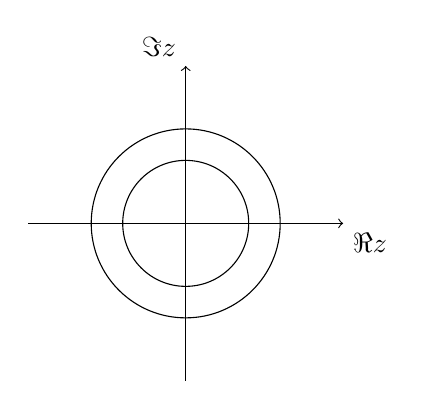
\begin{tikzpicture}[scale=1]
		\draw[->] (-2,0) -- (2,0) node[anchor=north west] {$\Re{z}$};
		\draw[->] (0,-2) -- (0,2) node[anchor=south east] {$\Im{z}$};
		\clip (-2,-2) rectangle (2,2);
		\draw (0,0) circle (1.2cm);
		\draw (0,0) circle (0.8cm);
		\end{tikzpicture}
	\end{center}
	Se per assurdo la serie converge in $z \implies$ per il teorema precedente  avremmo convergenza in ogni sfera con raggio minore di $\abs{\frac{1}{z}}$. e quindi anche in $w$ questo nega l'ipotesi.ASSURDO.
\end{proof}
\observation
Come è fatto l'insieme su cui si ha convergenza??\\
segue da queste due ultime proposizioni che se $\brackets{a_n:n\in\N}$ è una successione in $\C$ allora l'insieme $\brackets{z\in\C:\sum\limits_{n=0}^{+\infty}a_nz^n converge}$ è un cerchio.\\Sulla circonferenza non ci soffermiamo a capire cosa accade poiché tutto può accadere.
\definition
Raggio di convergenza della serie $\sum\limits_{n=0}^{+\infty}a_nz^n\bydef \rho=\sup\brackets{r \geq 0 :\sum\limits_{n=0}^{+\infty}a_nz^n converge su B(0,r)}$
\observation
Il raggio di convergenza di una serie di potenze può essere $0$, un numero reale positivo o $+\infty$.
\observation
una definizione come $\rho=\inf\brackets{r \geq 0 :\sum\limits_{n=0}^{+\infty}a_nz^n non converge su B(0,r)}$ non sta in piedi poiché questo insieme potrebbe essere vuoto, mentre quello sopra non è mai vuoto, perché $r=0$ c'è sempre poiché in $0$ si ha sempre convergenza. Il secondo potrebbe essere vuoto perché ci sono serie che convergono su tutto il piano complesso e quindi non si avrebbe nessun $r$ fuori da quale non sia ha convergenza.\\
\proposition CRITERIO DELLA RADICE.\\
Data la serie di potenze $\sum\limits_{n=0}^{+\infty}a_nz^n$, sia $l=\lim\limits_{n\to+\infty}\sqrt[n]{\abs{a_n}}$.\\
Se questo limite esiste, allora il raggio di convergenza è
$\rho =
	\begin{cases}
		0				&	\text{se }l=+\infty\\
		\frac{1}{l} 	&	\text{se }l\in\left]0,+\infty\right[\\
		+\infty 		& 	\text{se }l=0
	\end{cases}
$
\proposition CRITERIO DEL RAPPORTO.\\
Data la serie di potenze $\sum\limits_{n=0}^{+\infty}a_nz^n$, sia $l=\lim\limits_{n\to+\infty}\frac{a_{n+1}}{a_n}$.\\
Se questo limite esiste, allora il raggio di convergenza è
$\rho =
\begin{cases}
0				&	\text{se }l=+\infty\\
\frac{1}{l} 	&	\text{se }l\in\left]0,+\infty\right[\\
+\infty 		& 	\text{se }l=0
\end{cases}
$
ESEMPIO::$e^z=\sum\limits_{n=0}^{+\infty}\frac{1}{n!}z^n$\\
$a_n=\frac{1}{n!} ...  \abs{\frac{a_{n+1}}{a_n}}=\frac{\frac{1}{(n+1)!}}{\frac{1}{n!}}=\frac{n!}{(n+1)!}=\frac{1}{n+1}\overset{n\to+\infty}{\to}0 \implies \rho=+\infty$\\
ESEMPIO::$sin(z)=\sum\limits_{n=0}^{+\infty}\frac{(-1)^nz^{2n+1}}{(2n+1)!}$ quindi
$a_n =
\begin{cases}
0		&	\text{se }n\text{ è pari}\\
...		&	\text{se }n\text{ è dispari}\\
\end{cases}
$\\
...\\
...\\
...\\
ESEMPIO::$sin(z)=\sum\limits_{n=0}^{+\infty}\frac{(-1)^nz^{2n}}{(2n)!}$ quindi
$a_n =
\begin{cases}
...		&	\text{se }n\text{ è pari}\\
0		&	\text{se }n\text{ è dispari}\\
\end{cases}
$\\
...\\
...\\
...\\
ESEMPIO:: $e^{iy}$ con $y\in \R$
\[e^{iy} = \sum\limits_{n=0}^{+\infty}\frac{1}{n!}(iy)^n = \sum\limits_{n=0}^{+\infty}\frac{1}{(2n)!}(iy)^{2n} + \sum\limits_{n=0}^{+\infty}\frac{1}{(2n+1)!}(iy)^{2n+1} = \]
\[ = \sum\limits_{n=0}^{+\infty}\frac{(-1)^n}{(2n)!}(y)^{2n} + i\sum\limits_{n=0}^{+\infty}\frac{(-1)^n}{(2n+1)!}(y)^{2n+1} = cos(y)+i sin(y)\]
\begin{enumerate}
	\item $i^{2n}=\left(i^2\right)^n=(-1)^n$
	\item $i^{2n+1}=i\left(i^2\right)^n=i(-1)^n$
\end{enumerate}
ESEMPIO:: $e^{i\pi}+1=cos(\pi)+i\cdot sin(\pi)=0$\\
ESEMPIO:: $\sum\limits_{n=0}^{+\infty}z^n=\frac{1}{1-z}$ con $\rho=1$
ESEMPIO:: Sia $f(x)=\frac{1}{1+x^2}=\frac{1}{1-(-x^2)} = \sum\limits_{n=0}^{+\infty}(-x^2)^n=\sum\limits_{n=0}^{+\infty}(-1)^nx^{2n}$\\
QUI GRAFICO ..............\\
..........................\\
Questa serie converge esclusivamente per $\abs{x}<1$, mentre la funzione $f$ è definita su tutto $ \R$, $f\in \cntclass{\infty}( \R; \R)$\\
In $\C$, la funzione $f(z)=\frac{1}{1+z^2}$ è la somma della serie $\sum\limits_{n=0}^{+\infty}(-1)^nz^{2n}$ che ha raggio di convergenza  $\rho=1$. Infatti, $f(z)$ è singolare sia in $z=i$ sia in $z=-i$.\\
ALTRO GRAFICO::::::::::::::::\\
................................\\

\subsection{Serie di Taylor}
ESEMPIO:: $ln(1+z)$. Calcolare la Serie di Taylor.
\[D\left[ln(1+z)\right] = \frac{1}{1+z} = \sum\limits_{n=0}^{+\infty}(-1)^nz^n\]
\[\int \sum\limits_{n=0}^{+\infty}(-1)^nz^n dz = \sum\limits_{n=0}^{+\infty}\frac{(-1)^n}{n+1}z^{n+1}=\sum\limits_{n=1}^{+\infty}\frac{(-1)^{n-1}}{n}z^n\]
\begin{lemma}
	\label{lemma:taylor_rad_convergency}
	Sia $\brackets{a_n:n \in \N}$ una successione a valori in $\C$. Le serie:
	\[\sum_{n=0}^{+\infty} a_n z^n ,\qquad \sum_{n=1}^{+\infty} n a_n z^{n-1} \qquad\text{e}\qquad \sum_{n=0}^{+\infty} \frac{a_n}{n+1}z^{n+1}\]
	hanno lo stesso raggio di convergenza
	\begin{proof}
		Omessa
	\end{proof}
\end{lemma}

\definition
Sia $r\in \R$ con $r>0$. La funzione $f$ si dice analitica su $\left]-r,r\right[ \bydef f(x)=\sum\limits_{n=0}^{+\infty}a_nx^n \quad \forall x\in\left]-r,r\right[$ per opportuni $a_n\in \R$
\observation
In altre parole chiamiamo analitica una funzione che può essere scritta come somma di una serie di potenze convergente su $\left]-r,r\right[$ \\
ESEMPIO:: $x\to e^x$ è analitica su $ \R$\\
ESEMPIO:: $x\to\frac{1}{1+x^2}$ è analitica su $\left]-1,1\right[$\\
\proposition
Se $f$ è analitica su $\left]-r;r\right[$ per $r\in \R$ e $r>0 \implies f\in \cntclass{0}(\left]-r,r\right[; \R)$
\begin{proof}
	$f$ è analitica  allora posso scriverla come $f=\sum\limits_{n=0}^{+\infty}a_nx^n$ cioè la funzione è limite di una serie, se la serie converge totalmente allora converge uniformemente. Il limite uniforme di funzioni continue(in questo caso polinomi) è una funzione continua. cioè la $f$ è continua.
\end{proof}
\proposition PROP+PROOF\\
Sia $f:\left]-r,r\right[\to \R$ e $f$ analitica su $\left]-r,r\right[ \bydef f(x)=\sum\limits_{n=0}^{+\infty}a_nx^n \implies$ ho convergenza totale $\implies$ ho convergenza uniforme di funzioni continue
\[\implies f\in \cntclass{0}(\left]-r,r\right[; \R),\quad a_0=f(0)\]
La serie delle derivate $\sum\limits_{n=0}^{+\infty}na_nx^{n-1}$ converge totalmente su $\left]-r,r\right[$ cioè
\[\sum\limits_{n=0}^{+\infty}f'(x)=\sum\limits_{n=0}^{+\infty}na_nx^{n-1} \uconvarrow g\]
\[\sum\limits_{n=0}^{+\infty}fn(0)\to f(0), f_n\in ????????????\]
Allora la serie delle derivate converge alla derivata della serie
\[\implies \in \cntclass{1}(\left]-r,r\right[; \R),\quad a_1=f'(0)\]
Questo ragionamento può essere ripetuto:
\[\implies \forall k\in\N,\quad f\in \cntclass{k}(\left]-r,+r\right[),\quad a_k=k!f^{(k)}(0)\]
e analogamente
\[f\in \cntclass{\infty}(\left]-r,r\right[; \R),\quad f(x)=\sum\limits_{n=0}^{+\infty}\frac{1}{n!}f^{(n)}(0)x^n\]
\observation Qui abbiamo detto se $f$ è analitica $\implies \ldots$, vorrei fare un qualche tipo di viceversa per poter capire se $f$ è analitica o no.
\proposition
Sia $f:\left]-r,r\right[\to \R$
\begin{center}
	$\left.\begin{matrix}
	f\in \cntclass{\infty}(\left]-r,r\right[; \R)\\
	\sum\limits_{n=0}^{+\infty}\frac{1}{n!}f^{(n)}(0)x^n\text{ converge totalmente su } \left]-r,r\right[\\
	\end{matrix}\right\}\implies f$ è analitica  .....
\end{center}
Per avere $f$ analitica  necessariamente come ipotesi deve esserci $f\in \cntclass{\infty}$ e $f$ che si può scrivere come sviluppo in serie di Taylor,dalla proposizione precedente. Questo basta? NO\\
ESEMPIO:: $f(x)=\left\{\begin{matrix}0&& x=0\\e^{-\frac{1}{x^2}}&&x\ne 0\end{matrix}\right.$
\begin{center}
	\begin{tikzpicture}[scale=1]
	%\draw[->] (0,-4) -- (0,4) node[anchor=north west] {$x$};
	%\draw[->] (-0.1,0) -- (1.2,0) node[anchor=south east] {$y$};
	%\clip (-4,0) rectangle (4,1);
	%\draw[domain=-4:4,smooth,variable=\x] plot ({\x},{{-1/(\x*\x)}});
	\end{tikzpicture}
\end{center}
\begin{enumerate}
	\item $f\in \cntclass{\infty}( \R; \R)$
	\item $\sum\limits_{n=0}^{+\infty}\frac{1}{n!}f^{(n)}(0)x^n$ converge totalmente su $ \R$
	\item $f(x)\ne\sum\limits_{n=0}^{+\infty}\frac{1}{n!}f^{(n)}(0)x^n$
\end{enumerate}
\begin{enumerate}
	\item Vediamo se è $\cntclass{0}$, quindi calcolo $\lim\limits_{x\to 0^{+}}f(x)=\lim\limits_{x\to 0^{-}}f(x)=0=f(0)\implies f\in \cntclass{0}( \R; \R)$.\\
	Ora calcoliamo la derivata fuori dallo zero, ne facciamo il limite per $x\to 0$ da destra e da sinistra e vediamo cosa succede.\\
	Se $x\ne 0$, $f'(x)=\frac{2}{x^3}e^{-\frac{1}{x^3}}$ e $\lim\limits_{x\to 0^{+}}f'(x)=\lim\limits_{x\to 0^{-}} = 0 \implies f\in \cntclass{1}( \R; \R)$\\
	..........\\
	ancora una derivata.......\\
	..........\\
	Continuando a derivare  avremmo sempre un rapporto di polinomi che moltiplica un esponenziale, e l'esponenziale vince sempre. quindi fa $0$.
	itero il ragionamento......\\
	.......\\
	\item In (1) abbiamo visto  che tutte le derivate nello zero si annullavano, cioè
	\[\forall n\in\N, f^{(n)}(0)=0 \implies \sum\limits_{n=0}^{+\infty}\frac{1}{n!}f^{(n)}(0)x^n\]
	è la serie identicamente nulla  che banalmente converge totalmente su tutto $ \R$
	\item Anche osservandoli grafico è chiaro che la $f$ non è la funzione identicamente nulla cioè è diversa dal suo sviluppo in serie
	\[f(x)\ne\sum\limits_{n=0}^{+\infty}\frac{1}{n!}f^{(n)}(0)x^n\]
\end{enumerate}
Il Problema nasce dall'$o(x^n)$ che scriviamo alla fine dello sviluppo n-esimo di questa funzione, perché l'intorno in cui si ha $o(x^n)$ diventa sempre più piccolo.
GRAFICO...\\
GRAFICO...\\
Mandando l'ordine $n$ all'infinito, l'intervallo su cui si ha l'o piccolo tende a diventare un punto (lo zero). Quindi abbiamo l'uguaglianza tra la funzione e il suo sviluppo solo nell'origine.????????NON COMPRESA????\\
????????NON COMPRESA????\\
????????NON COMPRESA????\\
????????NON COMPRESA????\\
Completiamo le ipotesi con la prossima proposizione:
\proposition
Sia $f:\left]-r,r\right[\to \R$
\begin{center}
	$\left.\begin{matrix}
	f\in \cntclass{\infty}(\left]-r,r\right[; \R)\\
	\exists H,K >0 :\forall n\in\N \sup\limits_{\left]-r,r\right[}\abs{f^{(n)}(x)} \leq HK^n\\
	\end{matrix}\right\}
	\implies f(x)=\sum\limits_{n=0}^{+\infty}\frac{1}{n!}f^{(n)}(0)x^n$
\end{center}
\observation
L'ipotesi centrale ............. qui non c'è
\observation
Sia $\sum\limits_{n=0}^{+\infty}(z,w)^n$ una serie di potenze in due variabili.\\
Quando abbiamo due variabili, non si può parlare di raggio di convergenza. Questa serie è una serie geometrica che converge sse $\abs{zw}<1$. è  difficile parlare di raggio di convergenza  perché essendo $z,w\in\C$, se per una variabile servono due dimensioni per due variabili servono quattro dimensioni , e anche se non riusciamo a fare il disegno è evidente che l'insieme su cui la serie converge non è un cerchio(sfera).
\begin{example}[Esempi di Sviluppi in serie di Taylor]
	\label{ex:tay_series_examples}
	\begin{description}
		\item $e^x=\sum\limits_{n=0}^{+\infty}\frac{1}{n!}x^n$
		\item $sin(x)=\sum\limits_{n=0}^{+\infty}\frac{(-1)^n}{(2n+1)!}x^{(2n+1)}$
		\item $sinh(x)=\sum\limits_{n=0}^{+\infty}\frac{1}{(2n+1)!}x^{(2n+1)}$
		\item $cos(x)=\sum\limits_{n=0}^{+\infty}\frac{(-1)^n}{(2n)!}x^{(2n)}$
		\item $cosh(x)=\sum\limits_{n=0}^{+\infty}\frac{1}{(2n)!}x^{(2n)}$
		\item $\frac{1}{1-x}=\sum\limits_{n=0}^{+\infty}x^n$
		\item $ln(1+x)=\sum\limits_{n=1}^{+\infty}\frac{(-1)^{n+1}}{n}x^n$
		\item $arctan(1+x)=\sum\limits_{n=0}^{+\infty}\frac{(-1)^{n}}{2n+1}x^{(2n+1)}$
		\item $\frac{1}{1+x^2}=\sum\limits_{n=0}^{+\infty}(-1)^nx^2n$
		\item $\sum\limits_{n=0}^{+\infty}\frac{1}{n^\lambda}=\left\{\begin{matrix}\text{converge sse } \lambda >1\\ \text{diverge sse } \lambda  \leq 1 \end{matrix}\right.$
		\item $\sum\limits_{n=0}^{+\infty}q^n=\left\{\begin{matrix}\text{converge sse } \abs{q}<1, S=\frac{1}{1-x}\\ \text{diverge sse } \abs{q}>1\text{ o }q=1\\\nexists \text{ sse } x=-1 \end{matrix}\right.$
	\end{description}
\end{example}
\begin{exercise}
	\label{ex:deriv_func_with_taylor}
	Determinare le derivate delle funzioni
	\begin{itemize}[noitemsep]
		\item $x \to \sin x$
		\item $x \to \cos x$
		\item $x \to e^x$
	\end{itemize}
	utilizzando \fullref{ex:tay_series_examples}, il \fullref{lemma:taylor_rad_convergency} ed il \fullref{coro:deriv_serie_e_serie_derivate}.
\end{exercise}

\subsection{Serie di Fourier}
\definition
Siano $A\subseteq \R$, $f:A\to \R$ e $T>0$, $f$ è $T$-periodica $\bydef \forall x\in A
\left\{\begin{matrix}
x+T\in A\\f(x+T)=f(x)
\end{matrix}\right. $\\


ESEMPIO:: $\lfloor x \rfloor = \text{ parte intera } = \max\brackets{k\in\mathbb{Z}:k \leq x}$
\[\lfloor \pi \rfloor=3, \quad \lfloor \sqrt{2} \rfloor = 1 \quad \lfloor -e \rfloor = -3 \]
\begin{center}
	\begin{tikzpicture}
		\draw[->] (-4,0) -- (4,0) node[anchor=north west] {$x$};
		\draw[->] (0,-4) -- (0,4) node[anchor=south east] {$y$};

		\foreach \num in {-3,...,3} {
			\draw[line width=0.25mm] (\num , \num) -- (\num+1 , \num);
			\draw[fill=black] (\num , \num) circle (0.1cm);
			\draw (\num+1, \num) circle (0.1cm);
		}
	\end{tikzpicture}
\end{center}
è $1$-periodica.
ESEMPIO:: $mant(x)=\text{ mantissa di x } = x- \lfloor x \rfloor$
\begin{center}
	\begin{tikzpicture}
	\draw[->] (-4,0) -- (4,0) node[anchor=north west] {$x$};
	\draw[->] (0,-4) -- (0,4) node[anchor=south east] {$y$};

	\foreach \num in {-3,...,3} {
		\draw[line width=0.25mm] (\num , 0) -- (\num+1 , 1);
		\draw[fill=black] (\num , 0) circle (0.1cm);
		\draw (\num+1, 1) circle (0.1cm);
	}
	\end{tikzpicture}
\end{center}
è $1$-periodica.
\observation
La funzione costante è $T$-periodica $\forall T>0$, ma non ha un periodo minimo, per questo motivo non la consideriamo.
\observation
Sia $f:A\to \R$ $T$-periodica. Allora possiamo definire $\overline{f}:\overline{A}\to \R$ che sia $2\pi$-periodica data da:
\[x\to f\left(\frac{T}{2\pi}x\right),\quad \overline{A}=\frac{2\pi}{T}A\]
\proposition
Siano $A\subseteq \R$, $f:A\to \R$ e $T>0$\\
$f$ è $T$-periodica $\implies \forall n\in\N$, $f$ è $nT$-periodica.
\proposition
Sia $f:\left[0,2\pi\right[\to \R \implies \exists ! \hat{f}: \R\to \R$ t.c.: $\left\{\begin{matrix} \hat{f} 2\pi-periodica\\\hat{f}_{\left|\left[0,2\pi\right]\right.}=f\end{matrix}\right.$
\begin{proof}
	$\forall x\in \R. \exists ! \hat{x}\in\left[0,2\pi\right[$ t.c.: $x=2\pi\cdot k+\hat{x}$ con $k\in\mathbb{Z}$ e $k=\left[??????\right]$
	\[\hat{f}(x)=f(\hat{x})\]
\end{proof}
cioè se noi estendiamo una funzione definita su $\left[0,2\pi\right[$ a tutto $ \R$ otteniamo una funzione unica e periodica.
\observation
Con i polinomi di Taylor ........\\
........\\
........\\
........\\
........\\
........\\
\definition
Dati $2n+1$ numeri reali $a_0,a_1,\dotsc,a_n,b_1,\dotsc,b_n$ si dice polinomio trigonometrico di coefficienti $a_0,a_1,\dotsc,a_n,b_1,\dotsc,b_n$ la funzione:
\[\begin{array}{rcl} p: \left[-\pi,\pi\right] & \to &  \R \\ x & \to & \frac{a_0}{2}+\sum\limits_{k=1}^{N}\left(a_n cos(nx)+b_n sin(nx)\right) \end{array}\]
\observation
Essendo un'approssimazione, si deve aggiungere l'errore. Come è fatto?. Per far uscire conti giusti e comodi andrebbe usata la distanza quadratica , ma questo prevede una lunga parte introduttiva, noi allora lo stimiamo con la distanza infinita.
\definition
Date due successioni di numeri reali $\brackets{a_n:n\in\N}$,$\brackets{b_n:n\in\N\setminus\brackets{0}}$, si definisce serie trigonometrica di coefficienti  $\brackets{a_n:n\in\N}$,$\brackets{b_n:n\in\N\setminus\brackets{0}}$ la serie
\[\begin{array}{rcl} \mathfrak{F}: \left[-\pi,\pi\right] & \to &  \R \\ x & \to & \frac{a_0}{2}+\sum\limits_{k=1}^{+\infty}\left(a_n cos(nx)+b_n sin(nx)\right) \end{array}\]
LEMMA::\\
Se $h,k\in\N$ valgono le seguenti uguaglianze:
\begin{description}
	\item[$\ast$]
	$\int_{-\pi}^{\pi} cos(hx)cos(kx)=
	\left\{\begin{matrix}
	0 &&h\ne k\\\pi&&0\ne h=k\\2\pi&&0=h=k
	\end{matrix}\right.$
	\item[$\ast$] $\int_{-\pi}^{\pi}cos(hx)sin(kx)= 0 $
	\item[$\ast$]
	$\int_{-\pi}^{\pi}sin(hx)sin(kx)=
	\left\{\begin{matrix}
	0 &&h\ne k\text{ oppure }h=k=0\\ \pi&&0\ne h=k
	\end{matrix}\right.$
\end{description}
ESERCIZIO:: IL POLINOMIO DI FOURIER FORNISCE LA MIGLIORE APPROSSIMAZIONE NEL SENSO DELLA DISTANZA QUADRATICA.\\
Sia $f: \intervalclose{-\pi}{\pi} \to \R$, quale è la funzione a lei più vicina nel senso della distanza quadratica?\\
Fisso $N\in\N$ e prendo il polinomio trigonometrico di grado $N$
\[p_N(x)=\trigonpol{n}{1}{N}\]
con $a_0,a_1,\dotsc,a_n,b_1,\dotsc,b_n\in \R$, il problema è quello di minimizzare $d_2(f,p_n)$ quindi un problema di minimo. Stiamo cercando i coefficienti del polinomio trigonometrico quindi studiamo una funzione $\varphi(a_0,a_1,\dotsc,a_N,b_1,\dotsc,b_N) = \sqrt{\int_{-\pi}^{\pi}\left[f(x)-p_n(x)\right]^2}\integrald{x}$.\\
Essendo la funzione radice quadrata monotona crescente ne studiamo solo il radicando:
\[\varphi(a_0,a_1,\dotsc,a_N,b_1,\dotsc,b_N)=\int_{-\pi}^{\pi}\left[\trigonpol{n}{1}{N}-f(x)\right]^2dx\]
\observation
con $f\in \cntclass{1}$:
\[F(\alpha,\beta,x)=\int_{\alpha}^{\beta}f(x,t)\integrald{t}\]
\[\partial_\alpha F(\alpha,\beta,x)=-f(x,\alpha)\integrald{t}\]
\[\partial_\beta F(\alpha,\beta,x)=f(x,\beta)\integrald{t}\]
\[\nabla_x F(\alpha,\beta,x)=\int_{\alpha}^{\beta}\nabla_xf(x,t)\integrald{t}\]
Quindi applicando al nostro caso otteniamo
\[\partial_{a_0}\varphi = \int_{-\pi}^{\pi}\partial_{a_0}\left(\left[\trigonpol{n}{1}{N}-f(x)\right]^2\right)\integrald{x}=\]
\[ = \int_{-\pi}^{\pi} \frac{1}{2}2\left(\trigonpol{n}{1}{N}-f(x)\right)\integrald{x}=\]
\[ =  \int_{-\pi}^{\pi} \frac{a_0}{2}\integrald{x} + \]
\[\int_{-\pi}^{\pi} a_1cos(x)\integrald{x} +
\ldots +
\int_{-\pi}^{\pi} a_N cos(Nx)\integrald{x} + \]
\[\int_{-\pi}^{\pi} b_1sin(x)\integrald{x} +
\ldots +
\int_{-\pi}^{\pi} b_N sin(Nx)\integrald{x} - \]
\[ \int_{-\pi}^{\pi} f(x)\integrald{x} = \]
L'integrale di una sinusoide su un multiplo intero del periodo è $0$ quindi
\[=\pi a_0-\int_{-\pi}^{\pi}f(x)\integrald{x}\]
Calcolando direttamente anche le derivate seconde si ottiene che
\[\partial^2_{a_0a_0}=\pi\quad\partial^2_{a_0a_n}=0\quad\partial^2_{a_0b_n}=0\quad\forall n=1,\dotsc,N\]

\[\partial_{a_k}\varphi = \int_{-\pi}^{\pi}\partial_{a_k}\left(\left[\trigonpol{n}{1}{N}-f(x)\right]^2\right)\integrald{x}=\]
\[ = \int_{-\pi}^{\pi} 2cos(kx) \left[\trigonpol{n}{1}{N}-f(x)\right]\integrald{x}=\]
\[ =  \cancel{\int_{-\pi}^{\pi} a_0cos(kx)\integrald{x}} + \]
\[\cancel{\int_{-\pi}^{\pi} 2a_1cos(x)cos(kx)\integrald{x}} +
\ldots +
\int_{-\pi}^{\pi} 2a_k cos(kx)cos(kx)\integrald{x}
\ldots +
\cancel{\int_{-\pi}^{\pi} 2a_N cos(Nx)cos(kx)\integrald{x}} + \]
\[\cancel{\int_{-\pi}^{\pi} 2b_1sin(x)cos(kx)\integrald{x}} +
\ldots +
\cancel{\int_{-\pi}^{\pi} 2b_k sin(kx)cos(kx)}\integrald{x}
\ldots +
\cancel{\int_{-\pi}^{\pi} 2b_N sin(Nx)cos(kx)\integrald{x}} - \]
\[\int_{-\pi}^{\pi} 2f(x)cos(kx)\integrald{x} = \]
E anche applicando il lemma
\[=2\pi\left[a_k-\int_{-\pi}^{\pi}f(x)cos(kx)\integrald{x}\right]\]
Calcolando direttamente anche le derivate seconde si ottiene che
\[\partial^2_{a_ka_0}=\pi\quad\partial^2_{a_ka_n}=
\left\{\begin{matrix}
0&&n\ne k\\2\pi&&n=k
\end{matrix}\right.
\quad\partial^2_{a_kb_n}=0\quad\forall n=1,\dotsc,N\]

\[\partial_{b_k}\varphi = \int_{-\pi}^{\pi}\partial_{b_k}\left(\left[\trigonpol{n}{1}{N}-f(x)\right]^2\right)\integrald{x}=\]
\[ = \int_{-\pi}^{\pi} 2sin(kx) \left[\trigonpol{n}{1}{N}-f(x)\right]\integrald{x}=\]
\[ =  \cancel{\int_{-\pi}^{\pi} a_0sin(kx)\integrald{x}} + \]
\[\cancel{\int_{-\pi}^{\pi} 2a_1cos(x)sin(kx)\integrald{x}} +
\ldots +
\cancel{\int_{-\pi}^{\pi} 2a_k cos(kx)sin(kx)}\integrald{x}
\ldots +
\cancel{\int_{-\pi}^{\pi} 2a_N cos(Nx)sin(kx)\integrald{x}} + \]
\[\cancel{\int_{-\pi}^{\pi} 2b_1sin(x)sin(kx)\integrald{x}} +
\ldots +
\int_{-\pi}^{\pi} 2b_k sin(kx)sin(kx)\integrald{x}
\ldots +
\cancel{\int_{-\pi}^{\pi} 2b_N sin(Nx)sin(kx)\integrald{x}} - \]
\[\int_{-\pi}^{\pi} 2f(x)sin(kx)\integrald{x} = \]
E anche applicando il lemma
\[=2\pi\left[b_k-\int_{-\pi}^{\pi}f(x)cos(kx)\integrald{x}\right]\]
Calcolando direttamente anche le derivate seconde si ottiene che
\[\partial^2_{b_ka_0}=\pi\quad\partial^2_{b_ka_n}=
\left\{\begin{matrix}
0&&n\ne k\\2\pi&&n=k
\end{matrix}\right.
\quad\partial^2_{b_kb_n}=0\quad\forall n=1,\dotsc,N\]
Si verifica la condizione $\nabla\varphi = 0$ con
\begin{description}
	\item[$\ast$] $a_0=\frac{1}{\pi}\int_{-\pi}^{\pi}f(x)\integrald{x}$
	\item[$\ast$] $a_k=\frac{1}{\pi}\int_{-\pi}^{\pi}f(x)cos(kx)\integrald{x}$
	\item[$\ast$] $b_k=\frac{1}{\pi}\int_{-\pi}^{\pi}f(x)sin(kx)\integrald{x}$
\end{description}
La matrice Hessiana di $\varphi$ risulta \[H_{\varphi}=\left[\begin{matrix}
\pi&&0&&0&&\ldots&&0\\
0&&2\pi&&0&&\ldots&&0\\
0&&0&&2\pi&&\ldots&&0\\
\vdots&&\vdots&&\vdots&&\ddots&&\vdots\\
0&&0&&0&&0\ldots&&2\pi
\end{matrix}\right]\]
è una matrice diagonale quindi si leggono direttamente tutti gli autovalori che sono strettamente positivi quindi la forma quadratica è definita positiva ed il punto in questione è un punto di minimo assoluto.
\definition
Sia $f: \intervalclose{-\pi}{\pi} \to \R$, i coefficienti di Fourier di $f$ sono (ovviamente $f$ deve essere tale da ammetterli finiti):
\[a_0=\frac{1}{\pi}\int_{-\pi}^{\pi}f(x)\integrald{x}\]
\[a_k=\frac{1}{\pi}\int_{-\pi}^{\pi}f(x)cos(kx)\integrald{x}\quad k\in\N\setminus{\brackets{0}}\]
\[b_k=\frac{1}{\pi}\int_{-\pi}^{\pi}f(x)sin(kx)\integrald{x}\quad k\in\N\setminus{\brackets{0}}\]
La serie di Fourier di $f$ è
\[\trigonpol{k}{1}{+\infty}\]
\proposition
Sia $F: \intervalclose{-\pi}{\pi} \to \R$ la somma della serie trigono metrica definita dai coefficienti $\brackets{a_n:n\in\N}$ e $\brackets{a_n:n\in\N\setminus\brackets{0}}$ e la serie trigonometrica converge uniformemente allora $F$ è una funzione continua e
\[a_k=\frac{1}{\pi}\int_{-\pi}^{\pi}F(x)cos(kx)\integrald{x}\quad k\in\N\]
\[b_k=\frac{1}{\pi}\int_{-\pi}^{\pi}F(x)sin(kx)\integrald{x}\quad k\in\N\setminus{\brackets{0}}\]
ESEMPIO+DIMOSTRAZIONE:::\\
sia $f(x)=\trigonpol{n}{1}{+\infty}$. Allora:\\
\[a_0=\frac{1}{\pi}\int_{-\pi}^{\pi}f(x)\integrald{x}=\frac{1}{\pi}\int_{-\pi}^{\pi}\trigonpol{n}{1}{+\infty}\integrald{x}=\]
\[
= \frac{1}{\pi}\int_{-\pi}^{\pi}\frac{a_0}{2} +
\frac{1}{\pi}\int_{-\pi}^{\pi}\left(\sum\limits_{n=1}^{+\infty} a_n cos(nx)\right)\integrald{x} +
\frac{1}{\pi}\int_{-\pi}^{\pi}\left(\sum\limits_{n=1}^{+\infty} b_n cos(nx)\right)\integrald{x}
\]
Poiché si ha convergenza uniforme si può portare l'integrale dentro la sommatoria.
\[
= \frac{1}{\pi}\int_{-\pi}^{\pi}\frac{a_0}{2} +
\cancel{\frac{1}{\pi}\sum\limits_{n=1}^{+\infty}\int_{-\pi}^{\pi} a_n cos(nx)\integrald{x}} +
\cancel{\frac{1}{\pi}\sum\limits_{n=1}^{+\infty}\int_{-\pi}^{\pi} b_n cos(nx)\integrald{x}}=
\]
\[=\frac{1}{\pi}\frac{a_0}{2}\left(\pi-(-\pi)\right)=a_0\]


\[a_k=\frac{1}{\pi}\int_{-\pi}^{\pi}f(x)cos(kx)\integrald{x}=\]
\[\frac{1}{\pi}\left[
\cancel{\int_{-\pi}^{\pi}\frac{a_0}{2}cos(kx)\integrald{x}}+
\int_{-\pi}^{\pi}\left(\sum\limits_{n=1}^{+\infty}a_ncos(nx)cos(kx)\right)\integrald{x}+
\cancel{\int_{-\pi}^{\pi}\left(\sum\limits_{n=1}^{+\infty}b_nsin(nx)cos(kx)\right)\integrald{x}}
\right]=\]
\[\frac{1}{\pi}\left[
\cancel{\int_{-\pi}^{\pi}\left(\sum\limits_{n=1}^{k-1} a_ncos(nx)cos(kx)\right)\integrald{x}}+
\int_{-\pi}^{\pi}a_kcos(kx)cos(kx)\integrald{x}+
\cancel{\int_{-\pi}^{\pi}\left(\sum\limits_{n=k+1}^{+\infty}a_ncos(nx)cos(kx)\right)}\integrald{x}
\right]=\]
\[=\frac{1}{\pi}\pi a_k=a_k\]

\[b_k=\frac{1}{\pi}\int_{-\pi}^{\pi}f(x)sin(kx)\integrald{x}=\]
\[\frac{1}{\pi}\left[
\cancel{\int_{-\pi}^{\pi}\frac{a_0}{2}sin(kx)\integrald{x}}+
\int_{-\pi}^{\pi}\left(\sum\limits_{n=1}^{+\infty}a_ncos(nx)sin(kx)\right)\integrald{x}+
\cancel{\int_{-\pi}^{\pi}\left(\sum\limits_{n=1}^{+\infty}b_nsin(nx)sin(kx)\right)\integrald{x}}
\right]=\]
\[\frac{1}{\pi}\left[
\cancel{\int_{-\pi}^{\pi}\left(\sum\limits_{n=1}^{k-1} a_ncos(nx)sin(kx)\right)\integrald{x}}+
\int_{-\pi}^{\pi}a_kcos(kx)sin(kx)\integrald{x}+
\cancel{\int_{-\pi}^{\pi}\left(\sum\limits_{n=k+1}^{+\infty}a_ncos(nx)sin(kx)\right)}\integrald{x}
\right]=\]
\[=\frac{1}{\pi}\pi b_k=b_k\]
\observation
Se $d_2(f,\text{polinomio di Fourier})$ \`{e} minima $\implies$ il polinomio di Fourier \`{e} costruito con i coefficienti di Fourier di $f$.
\observation
Se $f$ \`{e} somma di una serie di funzioni $\implies$ i coefficienti della serie sono i coefficienti di Fourier.
\observation
Funzioni diverse possono avere gli stessi coefficienti di Fourier, cio\`{e} $\exists f,g$ con $f\ne g$ ma $f$ e $g$  hanno gli stessi coefficienti di Fourier.
ESEMPIO::
\begin{center}
	\begin{tikzpicture}
		\draw[->] (-2,0) -- (2,0) node [anchor=north west]{$x$};
		\draw[->] (0,0) -- (0,2);
		\clip (-2,0) rectangle (2,2);
		\draw[domain=-2:2,smooth,red,variable=\x] plot ({\x},{1}) node{$f$};
		\draw[domain=-2:2,smooth,blue,variable=\x] plot ({\x},{1}) node{$g$};
	\end{tikzpicture}
	SISTEMARE,
\end{center}
\observation
I coefficienti di Fourier non possono identificare univocamente puntualmente una funzione.
\subsubsection{Punto Di Vista Geometrico}
In $\R^2$ Ci sono $2$ vettori $\hat{i},\hat{j}$ della base, se $\underline{v}\in \R^2 \implies \underline{v}=v_1\cdot \hat{i}+v_2\cdot \hat{j}$ con $v_1,v_2$ componenti di $\underline{v}$\\
Calcolo delle componenti:
\[\underline{v}\cdot \hat{i} = v_1\cdot \hat{i\cdot }\hat{i}+v_2\cdot \hat{j}\cdot \hat{i}=v_1\]
\[\underline{v}\cdot \hat{j} = v_1\cdot \hat{i}\cdot \hat{j}+v_2\cdot \hat{j}\cdot \hat{j}=v_2\]
Questo vale perché $\hat{i},\hat{j}$ è una base ortonormale.
In $\R^3$ Ci sono $3$ vettori $\hat{i},\hat{j},\hat{k}$ della base, se $\underline{v}\in \R^3 \implies \underline{v}=v_1\hat{i}+v_2\hat{j}+v_3\hat{k}$ con $v_1,v_2,v_3$ componenti di $\underline{v}$\\
Calcolo delle componenti:
\[ v_1=\underline{v}\cdot \hat{i}\quad v_2=\underline{v}\cdot \hat{j}\quad v_3=\underline{v}\cdot \hat{k}  \]
In $\R^n$ Ci sono $n$ vettori $e_1,e_2,\dotsc,e_n$ della base, se $\underline{v}\in \R^n \implies \underline{v}=v_1\cdot e_1+v_2\cdot e_2+\ldots+v_n\cdot e_n=\sum\limits_{k=1}^{n}v_k\cdot e_k$ con $v_1,v_2,\dotsc,v_n$ componenti di $\underline{v}$\\
Calcolo delle componenti:
\[v_k=\underline{v}\cdot e_k\]
\\
Con le Serie di Fourier su esegue la stessa operazione sullo spazi $\cntclass{0}(\intervalclose{-\pi}{\pi}; \R)$. Come elementi di base si ha un insieme di funzioni:
\begin{enumerate}
	\item $c_0:x\to 1$
	\item $c_1:x\to cos(x)$
	\item $c_2:x\to cos(2x)$
	\item $\ldots$
	\item $c_n:x\to cos(nx)$
	\item $s_1:x\to sin(x)$
	\item $s_2:x\to sin(2x)$
	\item $\ldots$
	\item $s_n:x\to sin(nx)$
\end{enumerate}
Si possono osservare due cose:
\begin{enumerate}
	\item Sono tutte funzioni linearmente indipendenti, poiché l'unica combinazione lineare di questi elementi che da l'elemento nullo è quella a coefficienti tutti nulli.
\end{enumerate}
\definition
Il prodotto scalare in $\cntclass{0} \bydef \left<f,g\right>=\int_{-\pi}^{\pi}f(x)g(x)\integrald{x}$
Altre simbologie usate sono: $ f\bullet g $, $(f|g)$
\observation linearità
\[\left<(\alpha\cdot f+\beta\cdot g), h \right>= \int_{-\pi}^{pi} (\alpha\cdot f(x)+\beta\cdot g(x))\cdot h(x) \integrald{x}=\]
\[=\int_{-\pi}^{pi} \left[\alpha\cdot f(x)\cdot h(x)+\beta\cdot g(x)\cdot h(x) \right]\integrald{x}= \]
\[=\alpha\int_{-\pi}^{pi} \cdot f(x)\cdot h(x) \integrald{x}+\beta\int_{-\pi}^{pi} \cdot g(x)\cdot h(x) \integrald{x} =\]
\[\alpha\left<f,h\right>+\beta\left<g,h\right>\]

Ripetiamolo stesso ragionamento applicato in $ \R^2, \R^3,$ e $ \R^n$ per ricavare le componenti, possiamo fare questo perché abbiamo una base e abbiamo definito un prodotto scalare.\\
Se $f(x)=\trigonpol{n}{1}{+\infty} \implies $
\[a_0=\frac{1}{\pi}\int_{-\pi}^{\pi}f(x)dxs=\frac{1}{\pi}\left<f,c_0\right> \]
\[a_k=\frac{1}{\pi}\int_{-\pi}^{\pi}f(x)cos(kx)\integrald{x}=\frac{1}{\pi}\left<f,c_k\right> \]
\[b_k\frac{1}{\pi}\int_{-\pi}^{\pi}f(x)sin(kx)\integrald{x}=\frac{1}{\pi}\left<f,s_k\right>\]
Quindi come prima le componenti di un vettore si ottengono moltiplicando(prodotto scalare) il vettore per gli elementi della base.\\
PER IL LEMMA:\\
\[
\left<c_h,c_k\right>=
\left\{\begin{matrix}
0&&h\ne k\\
2\pi&&0=h=k\\
\pi&&0\ne h=k\\
\end{matrix}\right.
\]
\[ \left<c_h,s_k\right>=0\]
\[
\left<s_h,s_k\right>=
\left\{\begin{matrix}
0&&h\ne k\\
\pi&&0\ne h=k\\
\end{matrix}\right.
\]
Il prodotto scalare di elementi diversi è nullo quindi la base è ortogonale, ma non è ortonormale in quanto il prodotto scalare tra due elementi diversi della base non è unitario.(ecco perché gli $\frac{1}{\pi})$ e $\frac{a_0}{2}$)\\
In generale in geometria non è difficile normalizzare una base, è sufficiente dividere tutti gli elementi per la loro norma. In questo caso decidiamo di non applicare questo ragionamento poiché la norma vale $\sqrt{\pi}$ e se normalizziamo dobbiamo aggiungere questo termini ......\\
Il prodotto scalare in $\cntclass{0}$ è molto legato alla $d_2$ infatti:
\[\norm{f}_2=\sqrt{\left<f,f\right>}=\sqrt{\int_{-\pi}^{\pi}f(x)\cdot f(x)\integrald{x}}\sqrt{\int_{-\pi}^{\pi}\left[f(x)\right]^2dx}\]
Continuano le analogie:\\
In $ \R^2$ ........\\
In $ \R^3$ .........\\
.....\\
......\\
......\\
.....\\
Passando in dimensione infinita, abbiamo una funzione $f$ (come vettore $\underline{v}$) nello spazio, e fare il polinomio di Fourier  vuole dire proiettare la funzione $f$ in uno spazio fatto dai primi $2n+1$ elementi della base che è uno spazio di dimensione finita.\\
\\
Esempio:::: Non ogni funzione ammette coefficienti di Fourier finiti. La funzione
\[\begin{array}{rcl} f: \left[-\pi,\pi\right] & \to &  \R \\
x & \to & \left\{\begin{matrix} 0 && x=0\\\frac{1}{x^2}&&x\ne 0 \end{matrix}\right. \end{array}\]
non ammette coefficienti di Fourier finiti.\\
Esempio::: Una funzione può ammettere tutti i coefficienti di Fourier finiti ed una serie di Fourier convergente, ma ad un limite diverso da $f$.La funzione.
\[\begin{array}{rcl} f: \left[-\pi,\pi\right] & \to &  \R \\
x & \to & \left\{\begin{matrix} -1 && x<0\\1&&x>0 \end{matrix}\right. \end{array}\]
ha coefficienti di Fourier
\[a_k=0\quad\forall k,\qquad \left\{\begin{matrix}0 && k\text{ dispari }\\ \frac{4}{k\pi}&& k \text{ pari } \end{matrix}\right.\]
e serie di Fourier
\[ F_f(x)= \frac{4}{\pi}\sum\limits_{k=0}^{+\infty}\frac{sin(2h+1)x}{2h+1} \]
questa serie converge puntualmente in $0$ ma $F_f(0)\ne f(0)$\\

ESEMPIO:: Due funzioni diverse possono avere gli stessi coefficienti di Fourier:
\[\begin{array}{rcl} f: \left[-\pi,\pi\right] & \to &  \R \\
x & \to & \left\{\begin{matrix} -1 && x<0\\0&&x= 0\\1&&x>0 \end{matrix}\right.\end{array}\]
\[\begin{array}{rcl} g: \left[-\pi,\pi\right] & \to &  \R \\
x & \to & \left\{\begin{matrix} -1 && x<0\\\pi&&x= 0\\1&&x>0 \end{matrix}\right.\end{array}\]
\observation
Sia $f$ una funzione pari $\implies bn=0 \forall n=1,2,\dotsc,+\infty$
\observation
Sia $f$ una funzione dispari $\implies an=0 \forall n=0,1,,\dotsc,+\infty$
\observation
Siano
\[f(x)=\frac{a_0}{2}+\sum\limits_{n=}^{+\infty}\left(a_n cos(nx)+b_n sin(nx)\right)\]
\[\varphi(x)=\frac{\alpha_0}{2}+\sum\limits_{n=}^{+\infty}\left(\alpha_ncos(nx)+\beta_nsin(nx)\right)\]
Allora
\[ F(x)=(f+\varphi)(x)=\frac{A_0}{2}+\sum\limits_{n=}^{+\infty}\left(A_n cos(nx)+B_n sin(nx)\right)\]
con $A_n=a_n+\alpha_n$. $B_n=b_n+\beta_n$.
cioè i coefficienti di Fourier dipendono linearmente dalla funzione.\\
Esempio::: $B_3=\frac{1}{\pi}\int_{-\pi}^{\pi}F(x)sin(3x)\integrald{x}=\frac{1}{\pi}\int_{-\pi}^{\pi}(f(x)+\varphi(x))sin(3x)\integrald{x}=$\\
$\frac{1}{\pi}\left[\int_{-\pi}^{\pi}f(x)sin(3x)\integrald{x}+\int_{-\pi}^{\pi}\varphi(x)sin(3x)\integrald{x}\right]=b_3+\beta_3$\\
Sia $f(x)=\frac{a_0}{2}+\sum\liminf_{n=1}^{+\infty}\left(a_ncos(nx)+b_ncos(nx)\right)$ allora $F=4f=\frac{A_0}{2}+\sum\limits_{n=1}^{+\infty}\left(A_ncos(nx)+B_ncos(nx)\right)$ con $A_n=4a_n$, $B_n=4b_n$\\
ESEMPIO
Esempio:::$B_3=\frac{1}{\pi}\int_{-\pi}^{\pi}F(x)sin(3x)\integrald{x}=\frac{1}{\pi}\int_{-\pi}^{\pi}4f(x)sin(3x)\integrald{x}=4b_3$\\
\begin{definition}[Funzione Continua a Tratti]
	\index{Funzione!Continua a Tratti}
	Siano $a,b\in \R$ con $a<b$, una funzione $f:\intervalclose{a}{b} \to \R$. Allora $f$ è \textbf{continua a tratti} se esiste un numero finito di punti $x_1,x_2,\dotsc,x_n$ tali che:
	\begin{enumerate}
		\item In ogni punto di $\intervalclose{a}{b}\setminus\brackets{x_1,x_2,\dotsc,x_n}$ f è continua
		\item $i=1,2,\dotsc,n$ esistono finiti entrambi i limiti:
		\[\lim\limits_{x\to x_i^{-}}f(x)\quad \lim\limits_{x\to x_i^{+}}f(x)\]
	\end{enumerate}
\end{definition}

\observation
Dato $A\subseteq \R$ e data una funzione $f:A \to \R$, se $x_0$ è punto interno ad $A$, è comoda la notazione
\[f(x-)=\lim\limits_{\xi\to x^{-}}f(\xi)\quad f(x+)=\lim\limits_{\xi\to x^{+}}f(\xi)\]
Ovviamente se $f$ è continua in $x$ allora $f(x-)=f(x)=f(x+)$
ESEMPIII:::\\
GRAFICO::::\\
GRAFICO::::\\
.......\\
.......\\
.......\\
.......\\
\proposition
Sia $f: \intervalclose{-\pi}{\pi} \to \R$, $f$ è continua a tratti $\implies$ esistono finiti tutti i coefficienti di Fourier di $f$
\proposition
Sia $f: \intervalclose{-\pi}{\pi} \to \R$,\\
-$f$ è continua a tratti\\
-$\forall \overline{x} \in\intervalclose{-\pi}{\pi}$, esistono finiti:\\
\[ \lim\limits_{x\to\overline{x}^{-}}=\frac{f(x)-f(\overline{x}-)}{x-\overline{x}} \]
\[ \lim\limits_{x\to\overline{x}^{+}}=\frac{f(x)-f(\overline{x}+)}{x-\overline{x}} \]
Allora:\\
La serie di Fourier di $f$ converge puntualmente in $\overline{x}$ e $F_f(\overline{x})=\frac{f(\overline{x}-)-\overline{x}+}{2}$ (che è il punto medio del salto.)
\observation NIENTE CUSPIDI E NIENTE TANGENZE VERTICALI.

\corollary
Sia $f: \intervalclose{-\pi}{\pi} \to \R$,\\
$f$ è continua a tratti.\\
Sia $\overline{x}\in\intervalclose{-\pi}{\pi}$ un punto in cui $f$ è derivabile. Allora la serie di Fourier $F_f$ di $f$ converge in $\overline{x}$ e $F_f(\overline{x})=f(\overline{x})$
\proposition
Sia $f: \intervalclose{-\pi}{\pi} \to \R$.Se:\\
\begin{description}
	\item[$\ast$] $f\in \cntclass{0}(\intervalclose{-\pi}{\pi}; \R)$
	\item[$\ast$] $\exists x_1,x_2,\dotsc,x_n\in\intervalclose{-\pi}{\pi}$ t.c.:
	\begin{description}
		\item[-] $f$ è derivabile in $x$
		\item[-] $f'$ continua in $x$
	\end{description}
	\item[$\ast$] $\forall i=1,2,\dotsc,n$ e $\forall x\in\intervalclose{-\pi}{\pi}$ esistono finiti
	\[\lim\limits_{x\to x_i^{-}}\frac{f(x)-f(x_i-)}{x-x_i}\qquad \lim\limits_{x\to x_i^{+}}\frac{f(x)-f(x_i+)}{x-x_i}\]

\end{description}
Allora\\
La serie di Fourier $F_f$ di $f$ converge a $f$ uniformemente su $\intervalclose{-\pi}{\pi}$
\corollary
Sia $f: \intervalclose{-\pi}{\pi} \to \R$, e $f\in \cntclass{1}(\intervalclose{-\pi}{\pi}; \R)$.\\
Allora la serie di Fourier di $F_f$ di $f$ converge uniformemente a $f$ su $\intervalclose{-\pi}{\pi}$.
\chapter{Equazioni Differenziali}
\section{Preliminari}
Equazione è un uguaglianza in cui c'è almeno una incognita.\\
Equazione \textbf{Funzionale} è un’equazione le cui incognite sono funzioni.
\begin{note}
	In un equazione funzionale si cerca l'uguaglianza di: insieme di arrivo, insieme di partenza, corrispondenza.
\end{note}
Equazione \textbf{Differenziale} è un particolare tipo di equazione (funzionale) che stabilisce una relazione tra la funzione incognita e le sue derivate.

\begin{definition}[Equazione Differenziale Ordinaria]
	\index{Equazione!Differenziale Ordinaria}
	\label{def:equaz_diff}
	Si dice \textbf{Equazione Differenziale Ordinaria} (\textit{Ordinary Differential Equation, ODE}) \textbf{di ordine $n$} nella funzione incognita $x\in \R^k$ un espressione del tipo:
	\begin{equation}
		\label{eq:equaz_diff}
		f(t,x, x',\ldots,x^{(n)})=0
	\end{equation}
	\vspace*{-\baselineskip}
	\begin{note}
		La dipendenza delle $x$ dalla $t$ non è indicata esplicitamente, ma si potrebbe scrivere $x(t)$, rigorosamente nella stessa variabile $t$ per tutte le $x^{(i)}$.
	\end{note}
	La \cref{eq:equaz_diff} è $f: A \to \R^m$ con:
	\begin{itemize}[noitemsep]
		\item $A\subseteq \R^{1+(1+n)k}$
		\item $t\in I$ con $I$ intervallo $I \subseteq \R$
	\end{itemize}
	Dimensionalmente, si può osservare che $m$ e $k$ caratterizzano il problema e son dunque libere. La dimensione di partenza $1+(1+n)k$ del problema è obbligata e dovuta alla somma di:
	\begin{itemize}[noitemsep]
		\item $1 = \dim(t)$
		\item $(1+n)k$
		\begin{itemize}[noitemsep]
			\item $(1+n)$ il numero totale delle funzioni: $n$ derivate ed $x$ stessa
			\item $k$ la dimensione dell'insieme \textbf{di arrivo} di ogni funzione incognita $x^{(i)}$
		\end{itemize}
	\end{itemize}
	\begin{note}
		Alternativamente si può indicare $f$ come $f: \boldsymbol{I \times} A \to \R^m$ a patto di considerare $A\subseteq \R^{(1+n)k}$
	\end{note}
	\textbf{Soluzione} di questa equazione differenziale è una qualunque funzione $x:I\to \R^k$ (in quanto la $x$ è funzione di $t \in I$) definita sull'intervallo $I$, derivabile $n$ volte in $I$ (e dunque continua in $I$) e tale che $\forall t\in I$
	\[(t,x, x',\:\dotsc\:,x^{(n)}) \in A\]
	\[f(t,x, x',\:\dotsc\:,x^{(n)})=0\]
	\textbf{Soluzione massimale} di un equazione differenziale ordinaria è una soluzione $x_m:I_m\to \R^k$ tale che nessuna soluzione possa essere definita in un intervallo $I$ con $I_m\subseteq I$. Cioè è la soluzione definita sull'intervallo maggiore possibile.

	\begin{note} \hypertarget{def:equaz_diff_sol}{}
		Dalla definizione segue che $x(t) \in \circdot{A}$, in quanto se non fosse in $\circdot{A}$ sarebbe di frontiera, ma un punto di frontiera non può essere derivabile.
	\end{note}
	\begin{note}
		Un'equazione differenziale ammette, in generale, infinite soluzioni, come verificato in \fullref{ex:eq_diff_inf_sol}
	\end{note}
	\begin{note} \hypertarget{note:diff_eq_sol_definit_set}{}
		La soluzione di un'equazione differenziale può, analiticamente, essere definita su un intervallo $J\supset I$ ($I$ intervallo di definizione della funz. differenziale $f$). Non ha però senso considerare il suo comportamento al di fuori di $I$, in quanto non ha valore dal punto di vista del sistema. Per questo motivo $J$ sarà sempre considerato $J\subseteq I$
	\end{note}
	\begin{note}
		dalla \fullref{def:equaz_diff} segue che l'insieme di definizione della soluzione di un'equazione differenziale può essere solo un intervallo
	\end{note}
\end{definition}

\begin{example}
	\label{ex:eq_diff_inf_sol}
	Un'equazione differenziale ammette in generale infinite soluzioni. Ad esempio, $x' = 1$ è risolta da $x(t) = t + \alpha$ per qualunque $\alpha \in \R$
\end{example}
\begin{exercise}
	La soluzione di un'equazione differenziale ordinaria non può avere 3 asintoti.
	\begin{solution}
		La soluzione $x$ è funzione continua. In quanto continua non può avere più di 2 asintoti verticali e in quanto funzione non può avere più di 2 asintoti orizzontali.
	\end{solution}
\end{exercise}
\begin{definition}[Equazione Differenziale Ordinaria in Forma Normale]
	\index{Equazione!Differenziale Ordinaria!in Forma Normale}
	Un'equazione differenziale è in \textbf{Forma Normale} se e solo se si presenta nella forma 
	\[x^{(n)} = g(t,x, x',\:\dotsc\:,x^{(n-1)})\]
	Cioè se la derivata di ordine più alto è isolata al primo membro.
\end{definition}
\begin{observation}
	Lo studio di un'equazione differenziale ordinaria in forma non normale inizia generalmente con l'utilizzo del \fullref{teo:funz_impl} insieme ai teoremi sulle equazioni differenziali ordinarie in forma normale
\end{observation}
\begin{note}
	Nel seguito saranno considerate \textbf{solo} Equazioni Differenziali Ordinarie in Forma Normale.
\end{note}
\begin{proposition}
	\label{prop:equaz_n_equival_1}
	Ogni equazione differenziale ordinaria in forma normale di ordine $n$ è equivalente a una equazione differenziale ordinaria in forma normale di ordine $1$, cioè in cui compaiono solamente derivate prime.
	\begin{proof}
		Data l'equazione
		\[x^{(n)} = g(t,x, x', x'',\:\dotsc\:,x^{(n-1)})\]
		sia $y$ il vettore $y = \rvect{x &  x' &  x'' & \cdots & x^{(n-1)}}$. Abbiamo ora che le componenti del vettore sono
		\[y_1=x\qquad y_2= x'\qquad y_3= x''\qquad \dots\qquad y_n=x^{(n-1)}\]
		ed al contempo
		\[y_1'= x'=y_2\qquad y_2'= x''=y_3\qquad y_3'= x'''=y_4\qquad\cdots\qquad y_{n-1}'=x^{(n-1)}=y_n\]
		Cioè, differenziando l'$i$\textit{-esimo} elemento (che è una funzione) del vettore $y$, mi "sposto" all'elemento $i+1$ di $y$. A questo punto tutti gli elementi di $y$ sono equazioni differenziali del primo ordine.\\
		Quindi l'equazione può essere scritta come il seguente sistema del primo ordine
		\[\begin{cases}
			y_1'\quad=\quad y_2\\
			y_2'\quad=\quad y_3\\
			\vdots\\
			y_n' \quad = \quad g(t, y_1, y_2,\dots,y_n)
		\end{cases}\]
	\end{proof}
\end{proposition}
\begin{example}
	Posto $n=2$, si ha $x''=f(t, x, x')$.
	Come nella dimostrazione della \fullref{prop:equaz_n_equival_1}, si pongano
	\[X'= \begin{bmatrix} x'\\ x'' \end{bmatrix} \qquad \text{e} \qquad X=\begin{bmatrix}x\\ x'\end{bmatrix}\]
	Da cui $X'=f(t,X)$
\end{example}

\begin{definition}[Problema di Cauchy del Primo Ordine]
	\index{Problema di Cauchy!del Primo Ordine}
	\label{def:prob_cauchy_ord_1}
	Si dice Problema di Cauchy del Primo Ordine il problema di determinare una soluzione di un'equazione differenziale ordinaria del primo ordine, soddisfacente ad una condizione iniziale.
	\[\begin{cases}x'=f(t,x)\\x(t_0)=x_0\end{cases}\]
	Dove $f:I\times A\to \R^n$, $I\subseteq \R$ è un intervallo, $t_0\in\circdot{I}$, $A\subseteq \R^n$, $x_0\in\circdot{A}$.\\
	Soluzione di un problema di Cauchy è una funzione $x:J\to \R^n$, definita in un intervallo $J$ contenente $t_0$ nella sua parte interna, quindi $t_0\in J\subseteq I$.\\
	La funzione $x$ è soluzione dell'equazione differenziale $x'=f(t,x)$ ed è tale che:
	\begin{enumerate}
		\item $x(t_0)=x_0$
		\item $x(J)\subseteq A$
		\item $x$ derivabile (in quanto soluzione equazione differenziale)
	\end{enumerate}
	Quindi il problema di Cauchy aggiunge un vincolo ad un'equazione differenziale, così da isolare una singola soluzione.
\end{definition}
\begin{note}
	Si considera un intervallo perché l'idea è di studiare l'andamento nel tempo e sarebbe difficile far previsioni con "buchi" di tempo
\end{note}
\begin{note}
	La condizione $x(t_0) = x_0$ viene spesso definita condizione iniziale, malgrado la \fullref{def:prob_cauchy_ord_1} indichi che $t_0 \in \circdot{I}$, dunque a rigore non dovrebbe essere sulla frontiera di $I$. Questo è dovuto al fatto che, spesso, $t_0$ è proprio all'inizio dell'intervallo in cui si cerca la soluzione dell'equazione.\\
	Comunque i risultati esposti continuano a valere con piccole modifiche alle dimostrazioni.
\end{note}

\begin{definition}[Problema di Cauchy di Ordine $n$]
	\index{Problema di Cauchy!di Ordine $n$}
	Si dice problema di Cauchy di ordine $n$ il seguente problema:\\
	Determinare una soluzione di un'equazione differenziale ordinaria di ordine $n$ soddisfacente a $n$ condizioni iniziali:
	\[\begin{cases}
		x^{(n)}=f(t,x,x',\dotsc,x^{(n-1)})\\
		x(t_0)=\alpha_0\\
		x'(t_0)=\alpha_1\\
		\vdots\\
		x^{(n-1)}(t_0)=\alpha_{n-1}
	\end{cases}\]
\end{definition}
\begin{note}
	Le condizioni iniziali \textbf{devono} essere assegnate tutte nello \textbf{stesso istante}, altrimenti il problema fornito non sarebbe un Problema di Cauchy, stando alla definizione fornita sopra.
\end{note}
\begin{example}
	il problema di Cauchy \[\begin{cases}x'=x\\x(0)=1\end{cases}\]
	ammette, tra le altre, anche le seguenti soluzioni, tecnicamente distinte tra loro
	\[\funcdef{f_1}{ \intervalclose{-1}{1} }{\R}{t}{e^t} \qquad \funcdef{f_2}{ \intervalclose{-2}{10} }{\R}{t}{e^t}\]
	La soluzione massimale è
	\[\funcdef{f_M}{\R}{\R}{t}{e^t}\]
	con intervallo di partenza $\R$, avente evidentemente diametro maggiore possibile.
\end{example}
\begin{proposition}
	Ogni problema di Cauchy di ordine $n$ è equivalente ad un problema di Cauchy del primo ordine
	\begin{proof}
		Dalla \fullref{prop:equaz_n_equival_1}
	\end{proof}
\end{proposition}

\begin{proposition}
	Ogni problema di Cauchy del primo ordine con secondo membro continuo
	\[\begin{cases}x'=f(t,x)\\x(t_0)=x_0\end{cases}\]
	è equivalente ad un'equazione integrale del tipo
	\begin{equation}
		\label{eq:volterra}
		x(t)=x_0+\int_{t_0}^{t}\Bigl(f\bigl(\tau,x(\tau)\bigr)\Bigr)\integrald{\tau}
	\end{equation}
	\begin{proof}
		Integrando ambo i membri della prima equazione del problema di ottiene:
		\[\int_{t_0}^{t}( x')\integrald{\tau}=\int_{t_0}^{t}(f(\tau,x(\tau)))\integrald{\tau}\]
		\[x(t)-x(t_0)=\int_{t_0}^{t}(f(\tau,x(\tau)))\integrald{\tau}\]
		\[x(t)=x_0+\int_{t_0}^{t}(f(\tau,x(\tau)))\integrald{\tau}\]
	\end{proof}
\end{proposition}
\begin{definition}[Equazione di Volterra]
	\index{Equazione!di Volterra}
	\label{def:equaz_volterra}
	La \cref{eq:volterra} viene denominata \textbf{equazione integrale di Volterra}.
\end{definition}
\begin{note}
	\hypertarget{note:volterra_non_cont}
	Questa equazione ha senso anche per alcune funzioni $f$ non non continue, ma solo misurabili nel primo argomento. Ne consegue che nei Teoremi di esistenza ed unicità (locali/globali) l'ipotesi ``$f$ continua'' può essere sostituita da ``$f$ continua a tratti in $t, \forall x$, continua in $x$ e limitata''.
\end{note}

\begin{example}[Un Problema di Cauchy senza soluzione]
	Sia
	\[\funcdef	{f}
				{\R}
				{\R}
				{x}
				{	\begin{cases}
						\begin{array}{ll}
							+1 & \text{se } x < 0\\
							-1 & \text{se } x \geq 0
						\end{array}
					\end{cases}}\]
	Allora il Problema di Cauchy
	\[\begin{cases}
		x'=f(x)\\
		x(0) = 0
	\end{cases}\]
	Non ammette soluzioni. %  perché la condizione $x(0) = 0$ non è mai verificata.

	\begin{solution}
		~
		\begin{center}
			\begin{tikzpicture}
				\begin{axis} [
					axis lines = center,
					ymin = -2, ymax = 2
				]
					\addplot[domain=-2:0, thick] {1};
					\addplot[domain=0:2, thick] {-1};
					\addplot[color=black, only marks, mark=*] coordinates {(0, -1)};
					\addplot[color=black, fill=white, only marks, mark=*] coordinates {(0, 1)};
				\end{axis}
			\end{tikzpicture}
		\end{center}
		La $f$ è definita su tutto $\R$, ma non è possibile trovare una funzione di primo grado, derivabile su tutto $\R$, la cui derivata prima assuma quei valori. Infatti la
		\[\begin{cases}
			\begin{array}{ll}
				x & \text{se } t < 0\\
				-x & \text{se } t \geq 0
			\end{array}
		\end{cases}\]
		non è derivabile in $t = 0$, perché le derivate destra e sinistra assumono valori diversi.
	\end{solution}
\end{example}
\begin{example}[Un Problema di Cauchy con infinite soluzioni]
	Sia
	\[\funcdef{f}{\R}{\R}{x}{\sqrt{\abs{x}}}\]
	Allora il Problema di Cauchy
	\begin{equation*}
		\begin{cases}
			x' = \sqrt{\abs{x}}\\
			x(0) = 0
		\end{cases}
	\end{equation*}
	ammette le infinite soluzioni
	\begin{equation*}
		x_{a,b}(t) =
		\begin{cases}
			\begin{array}{ll}
				-\frac{1}{4}(t-a^2) & \text{se } t \in \intervalopcl{-\infty}{a}\\
				0 & \text{se } t \in \intervalclose{a}{b}\\
				\frac{1}{4}(t-b^2) & \text{se } t \in \intervalclop{b}{+\infty}
			\end{array}
		\end{cases}
	\end{equation*}
	dove $-\infty \leq a \leq 0 \leq b \leq +\infty$
	\begin{solution}
		Vedere \fullref{ex:pennello_peano} con $x_0 = 0$ e $t_0 = 0$
	\end{solution}
\end{example}
\begin{observation}
	Negli esempi precedenti è stata sfruttata la mancanza di regolarità nella dipendenza di $f$ da $x$.

	Viceversa, nella \hyperlink{note:volterra_non_cont}{\notestyle{} alla \fullref*{def:equaz_volterra}}, si era notato come la dipendenza di $f$ da $t$ sia molto meno critica.
\end{observation}
\begin{exercise}
	Sia $s:\R \to \R$ data da
	\[s(t) =
	\begin{cases}
		1 \qquad \text{se } t \geq 0\\
		0 \qquad \text{se } t < 0
	\end{cases}\]
	Risolvere i seguenti Problemi di Cauchy, al variare di $t_0$ (si supponga $t_0 \neq 0,1$):

	\begin{minipage}{0.48\linewidth}
		\begin{align*}
			&\begin{cases}
				x' = s(t)\\
				x(t_0) = 1\\
			\end{cases}\\
			&\begin{cases}
				x' = s(t) \cdot s(1-t)\\
				x(t_0) = 1\\
			\end{cases}
		\end{align*}
	\end{minipage}
	\begin{minipage}{0.48\linewidth}
		\begin{align*}
			&\begin{cases}
				x' + x = s(t)\\
				x(t_0) = 1\\
			\end{cases}\\
			&\begin{cases}
				x' - x = s(t) \cdot s(1-t)\\
				x(t_0) = 1\\
			\end{cases}
		\end{align*}
	\end{minipage}
	% TODO solution
\end{exercise}
\begin{example}[Un Problema non di Cauchy]
	Il seguente è un \textbf{Problema ai Valori al Contorno} e non un Problema di Cauchy, in quanto:
	\begin{itemize}[noitemsep]
		\item le condizioni iniziali non sono valutate nello stesso istante.
		\item le condizioni iniziali sono ai margini dell'insieme di definizione della funzione soluzione (che si vedrà sotto)
	\end{itemize}
	\begin{equation}
		\label{eq:probl_val_contorno}
		\begin{cases}
			x'' + x = 0\\
			x(0) = 0\\
			x(\pi) = 0
		\end{cases}
	\end{equation}
	Questo problema ammette le infinite soluzioni $x(t) = \alpha \cdot \sin t$, al variare di $\alpha \in \R$.

	Se venissero sostituite le condizioni di \cref{eq:probl_val_contorno} con $x(0) = x(\frac{\pi}{2}) = 1$ si otterrebbe l'unica soluzione $x(t) = \sin t + \cos t$. Con le $x(0) = x(\pi) = 1$ assegnate, invece, non ci sono soluzioni.
\end{example}

\begin{samepage}
\begin{observation}[Problema ben posto nel senso di Hadamard]
	\label{obs:hadamard}
	\index{Problema Ben Posto}
	in generale un problema si dice \textbf{ben posto} o \textbf{ben posto nel senso di Hadamard} ogniqualvolta la soluzione:
	\begin{enumerate}
		\item esiste
		\item è unica
		\item dipende con continuità dai dati
	\end{enumerate}
\end{observation}
\end{samepage}

\newpage
\section{Teoria Locale}
\begin{definition}[Funzione Localmente Lipschitziana]
	\index{Funzione!Localmente Lipschitziana}
	\label{def:loc_lips}
	Una funzione $f:I\times A\to \R^n$, con $I$ intervallo in $\R$ e $A$ aperto in $\R^n$, si dice \textbf{Localmente lipschitziana} in $x\in A$ \textbf{uniformemente} rispetto a $t \in I$ se
	\[\forall x_0 \in A,\; \exists r > 0 \text{ e } \exists L > 0:\quad \forall x_1,x_2 \in (B(x_0,r)\cap A),\; \forall t\in I\]
	\hfil vale che
	\[
		\norm{f(t,x_2)-f(t,x_1)}\leq L\cdot\norm{x_2-x_1}
		\qquad\text{o, ugualmente}\qquad
		\frac{\norm{f(t,x_2)-f(t,x_1)}}{\norm{x_2-x_1}}\leq L
	\]
	Una funzione è uniformemente lipschitziana (\textbf{unif. lips.}) in un'intervallo $I$ se, in parole povere, è possibile individuare per ogni punto di $I$ una sfera $B$ di raggio $r$ in cui la funzione è lipschitziana.
\end{definition}
\begin{note}
	I termini \textit{localmente} e \textit{uniformemente} son giustificati dal fatto che:
	\begin{itemize}[noitemsep]
		\item La località è data dalla limitazione di $x_1,x_2$ all'interno di $(B(x_0,r)\cap A)$
		\item L'uniformità è data da $\forall t\in I$
	\end{itemize}
	Quindi la $f$ rimane lips. indipendentemente dalla variazione di $t$ (quindi $\forall t\in I$), ma solo per $x_1,x_2 \in (B(x_0,r)\cap A)$, \textbf{non} $\forall x\in A$.
\end{note}
\begin{note}
	\hypertarget{note:if_lips_then_loclips}
	Se $f$ \textbf{lips} su $A\implies f$ \textbf{loc. lips.} su A.\\
	Concettualmente ci si porta nel caso della sfera $B$ con $r$ pari al raggio di $I\times A$ su cui è definita $f$
\end{note}
\begin{example}
	\label{ex:loc_lips_graphs}

	~
	\begin{figure}[H]
		\begin{subfigure}{.24\textwidth}
			\centering
			\resizebox{\linewidth}{!}{
				\begin{tikzpicture}
					\begin{axis} [
						axis lines = center,
						axis on top=true,
						legend style={empty legend}
					]
						\addplot [domain=-3:-.2,samples=50] {exp(ln(abs(x))/3)};
						\addplot [domain=-.2:.2,samples=100,smooth] {exp(ln(abs(x))/3)};
						\addplot [domain=.2:3,samples=50] {exp(ln(abs(x))/3)};
						\addlegendentry{\raisebox{.5ex}{$\sqrt[3]{\abs{x}}$}}
					\end{axis}
				\end{tikzpicture}
			}
			\caption{No Loc. lips.\\ No lips.}
		\end{subfigure}
		\begin{subfigure}{.24\textwidth}
			\centering
			\resizebox{\linewidth}{!}{
				\begin{tikzpicture}
					\begin{axis} [
						axis lines = center,
						axis on top=true,
						legend style={empty legend}
					]
						\addplot [domain=-3:3,samples=100] {abs(x)};
						\addlegendentry{\raisebox{.5ex}{$\abs{x}$}}
					\end{axis}
				\end{tikzpicture}
			}
			\caption{Sì loc. lips.\\ Sì lips.}
		\end{subfigure}
		\begin{subfigure}{.24\textwidth}
			\centering
			\resizebox{\linewidth}{!}{
				\begin{tikzpicture}
					\begin{axis} [
						axis lines = center,
						axis on top=true,
						legend style={empty legend}
					]
						\addplot [domain=-2:2,samples=100] {x^2};
						\addlegendentry{\raisebox{.5ex}{$x^2$}}
					\end{axis}
				\end{tikzpicture}
			}
			\caption{Sì loc. lips.\\ No lips.}
		\end{subfigure}
		\begin{subfigure}{.24\textwidth}
			\centering
			\resizebox{\linewidth}{!}{
				\begin{tikzpicture}
					\begin{axis} [
						axis lines = center,
						axis on top=true,
						ymin = -1.2, ymax = 1.2,
						legend style={empty legend}
					]
						\addplot[domain=-1:-.2,samples=50,smooth]{sin(deg(1/x))};
						\addplot[domain=-.2:-.0001,samples=1000]{sin(deg(1/x))};
						\addplot[domain=.0001: 0.2,samples=1000]{sin(deg(1/x))};
						\addplot[domain=.2: 1,samples=50,smooth]{sin(deg(1/x))};
						\addlegendentry{\raisebox{.5ex}{$\sin \frac{1}{x}$}}
					\end{axis}
				\end{tikzpicture}
			}
			\caption{Sì loc. lips.\\ No lips.}
		\end{subfigure}
	\end{figure}
\end{example}
\begin{example}
	La funzione $f:\R\to \R$ data da $f(x)=x^2$ è \textbf{loc. lips.} su $\R$ ma non è \textbf{globalmente lips.} su $\R$. Vedasi \fullref{def:lips} e grafico della $f$ in \fullref{ex:loc_lips_graphs}
\end{example}

\begin{proposition}
	\label{prop:fc1_loc_lips}
	Siano $I\subseteq \R$ un intervallo aperto e $A\subseteq \R^n$ un aperto. Ogni funzione $f\in\cntclass{1}(I\times A;\R^n)$ è loc. lips. in $x\in A$ uniformemente rispetto a $t\in I$
	\begin{proof}
		Il prodotto cartesiano $I\times A$, essendo prodotto cartesiano di aperti in $\R^n$ con metrica euclidea (si suppone sia in uso questa metrica), è a sua volta un aperto. Questo risultato è dovuto alla definizione stessa del prodotto cartesiano di $\R$ con metrica euclidea.\\
		% TODO Magari scrivere proposizione prodotto cartesiano di aperti = aperto.
		Chiamiamo ora $S=I\times A$ l'insieme di partenza della $f$. Grazie alla \fullref{prop:polig_in_aperto_connesso} sappiamo che esiste una poligonale interamente contenuta in $S$ congiungente due qualunque punti dell'aperto $S$.\\
		È ora possibile applicare il \fullref{teo:accresc_fin} ad uno qualunque dei segmenti formanti la poligonale appena individuata. Vale quindi la
		\[\norm{f(x_1)-f(x_0)} \leq \sup\limits_{x\in S}\norm{Df(x)}\norm{x_1-x_0}\]
		che è direttamente comparabile alla \fullref{def:loc_lips} della funzione in ciascuno dei segmenti della poligonale, da cui la tesi.
	\end{proof}
\end{proposition}

\subsection{Esistenza e Unicità}
\begin{theorem}[di Peano]
	\index{Teorema!di Peano}
	\label{teo:peano}
	Si consideri il seguente problema di Cauchy:
	\[\left\{\begin{matrix} x'=f(t,x)\\x(t_0)=x_0\end{matrix}\right.\]
	con $f:I\times A \to \R^n$ soddisfacente alle ipotesi:
	\begin{enumerate}
		\item $I$ intervallo, $I \subseteq \R$ e $A\subseteq \R^n$ per \fullref{def:prob_cauchy_ord_1}
		\item $t_0\in \circdot{I},\: x_0\in \circdot{A}$
		\item $f\in \cntclass{0}(I\times A;\R^n)$
	\end{enumerate}
	Allora $\exists \delta > 0$ per cui esista la soluzione $x: J \to A$ del Problema di Cauchy con $J = \intervalclose{t_0-\delta}{t_0+\delta}$.
	\begin{note}
		$\delta$ è un valore arbitrario che serve solo ad identificare l'intervallo $J$ a cui appartiene $t_0$, non è dato modo per identificare quel $\delta$
	\end{note}
	\begin{proof}
		Non richiesta
	\end{proof}
\end{theorem}
\begin{example}[Il Baffo/Pennello di Peano]
	\label{ex:pennello_peano}
	\index{Baffo di Peano}
	\index{Pennello di Peano}
	Trovare le soluzioni del Problema di Cauchy
	\begin{equation*}
		\begin{cases}
			x' = \sqrt{\abs{x}}\\
			x(t_0) = x_0
		\end{cases}
	\end{equation*}

	\begin{solution}
		~
		\begin{figure}[H]
			\begin{subfigure}{.49\textwidth}
				\centering
				\resizebox{\linewidth}{!}{
					\begin{tikzpicture}
						\begin{axis} [
							axis lines = center,
							axis on top=true,
							axis equal,
							xlabel = $x$,
							ylabel = {$x'$},
						]
						\addplot [domain=-5:-.5, samples=50, smooth] {(abs(x))^(1/2)};
						\addplot [domain=-.5:.5, samples=200, smooth] {(abs(x))^(1/2)};
						\addplot [domain=.5:5, samples=50, smooth] {(abs(x))^(1/2)};
						\end{axis}
					\end{tikzpicture}
				}
			\end{subfigure}
			\begin{subfigure}{.49\textwidth}
				\centering
				\resizebox{\linewidth}{!}{
					\begin{tikzpicture}
						\begin{axis} [
							axis lines = center,
							axis on top=true,
							axis equal,
							xlabel = $t$,
							ylabel = {$x(t)$},
							legend style={at={(0.2,0.7)},anchor=south},
						]
						\addplot [domain=-5:0, samples=50, smooth, forget plot] {-1/4*x^2};
						\addplot [domain=0:5, samples=50, smooth] {1/4*x^2};
						\addlegendentry{$t_0 = 0$}
						\addplot [domain=-5:0, samples=50, smooth, color=blue, forget plot] {1 + -1/4*x^2};
						\addplot [domain=0:5, samples=50, smooth, color=blue] {1 + 1/4*x^2};
						\addlegendentry{$t_0 = 1$}
						\addplot [domain=-5:0, samples=50, smooth, color=red, forget plot] {-1 + -1/4*x^2};
						\addplot [domain=0:5, samples=50, smooth, color=red] {-1 + 1/4*x^2};
						\addlegendentry{$t_0 = -1$}
						\end{axis}
					\end{tikzpicture}
				}
				\caption{Posto $x_0 = 0$}
			\end{subfigure}
		\end{figure}
		\begin{note}
			L'equazione differenziale non dipende da $t$, quindi il sistema è \textbf{Autonomo}. Vedere le note a \fullref{def:equaz_diff_auton} per le implicazioni concettuali.
		\end{note}
		\begin{note}
			Con $x_0 = 0$ si ha $x(t)=0$, che è soluzione $\forall t$, si procede però nel cercare altre soluzioni.
		\end{note}
		$f$ è continua $\forall x \in \R$, dunque per \fullref{teo:peano} esiste una soluzione del Problema. Essendo $x' = \sqrt{\abs{x}}$ un'equazione a variabili separabili, si ottiene (considerando $x \geq 0$, quindi $\abs{x} = x$):
		\begin{equation*}
			\begin{gathered}
				\frac{x'}{\sqrt{x}} = 1\\
				\int_{t_0}^{t}{\frac{x'(\tau)}{\sqrt{x(\tau)}}\integrald{\tau}} = \int_{t_0}^{t} 1 \integrald{\tau}\\
				2\bigl(\sqrt{x(t)} - \sqrt{x(t_0)}\bigr) + c_1 = t - t_0 + c_2\\
			\end{gathered}
		\end{equation*}
		Riunendo $c_1$ e $c_2$ in un'unica costante $b$
		\begin{gather*}
			2\bigl(\sqrt{x(t)} - \sqrt{x(t_0)}\bigr) + b = t - t_0\\
			2\bigl(\sqrt{x(t)} - \sqrt{x(t_0)}\bigr) = t - t_0 - b\\
			x_a(t) = \left( \sqrt{x_0} + \frac{1}{2}(t-t_0-b) \right)^2\\
			x_a(t) = x_0 + \sqrt{x_0} \cdot (t-t_0-b) + \frac{1}{4}(t-t_0-b)^2
		\end{gather*}
		Aggiungendo anche la soluzione per $x < 0$ (con la costante $a$, stavolta), si ottiene
		\begin{equation*}
			x_{a,b}(t) =
			\begin{cases}
				\begin{array}{ll}
					% TODO controllare i segni dell'equazione per t < a. Il primo - serve?
					x_0 - \sqrt{x_0} \cdot (t-t_0-a) - \frac{1}{4}(t-t_0-a)^2 & \text{se } t \in \intervalopcl{-\infty}{a}\\
					x_0 & \text{se } t \in \intervalclose{a}{b}\\
					x_0 + \sqrt{x_0} \cdot (t-t_0-b) + \frac{1}{4}(t-t_0-b)^2 & \text{se } t \in \intervalclop{b}{+\infty}
				\end{array}
			\end{cases}
		\end{equation*}
		Abbiamo quindi trovato infinite soluzioni, ciò evidenzia come il teorema di Peano non garantisca affatto unicità.
		\begin{figure}[H]
			\begin{subfigure}{.49\textwidth}
				\centering
				\resizebox{\linewidth}{!}{
					\begin{tikzpicture}
						\begin{axis} [
							axis lines = center,
							axis equal,
							ymin = -6,
							ymax = 6,
							xlabel = $t$,
							ylabel = {$x(t)$},
							legend style={at={(0.2,0.7)},anchor=south},
						]
						\addplot [domain=-8:-3, samples=50, smooth, forget plot, color = red] {-1/4*(x + 3)^2};
						\addplot [domain=-3:4, samples=50, smooth, forget plot, color = red] {0};
						\addplot [domain=4:8, samples=50, smooth, color = red] {1/4*(x - 4)^2};
						\addlegendentry{$a = -3, b = 4$}
						\addplot [domain=-8:-1, samples=50, smooth, forget plot, color = blue] {-1/4*(x + 1)^2};
						\addplot [domain=-1:1, samples=50, smooth, forget plot, color = blue] {0};
						\addplot [domain=1:8, samples=50, smooth, color = blue] {1/4*(x - 1)^2};
						\addlegendentry{$a = -1, b = 1$}
						\addplot [domain=-8:0, samples=50, smooth, forget plot] {-1/4*(x)^2};
						\addplot [domain=0:8, samples=50, smooth] {1/4*(x)^2};
						\addlegendentry{$a = 0, b = 0$}
						\end{axis}
					\end{tikzpicture}
				}
				\caption{Differenti valori di $a$ e $b$}
			\end{subfigure}
			\begin{subfigure}{.49\textwidth}
				\centering
				\resizebox{\linewidth}{!}{
					\begin{tikzpicture}
						\begin{axis} [
							axis lines = center,
							axis equal,
							ymin = -6,
							ymax = 6,
							xlabel = $t$,
							ylabel = {$x(t)$},
							legend style={at={(0.2,0.7)},anchor=south},
						]
						\pgfplotsinvokeforeach{-4,-3.5,...,0} {
							\addplot [domain=-8:#1, samples=50, smooth, forget plot] {-1/4*(x - #1)^2};
						}
						\pgfplotsinvokeforeach{0,.5,...,4} {
							\addplot [domain=#1:8, samples=50, smooth, forget plot] {1/4*(x - #1)^2};
						}
						\end{axis}
					\end{tikzpicture}
				}
				\caption{Il comportamento "a pennello" con molteplici $a$ e $b$}
			\end{subfigure}
			\caption{Grafici tracciati con $x_0 = 0$ e $t_0 = 0$}
		\end{figure}
	\end{solution}
\end{example}

\begin{theorem}[di Cauchy Locale - Prima Parte]
	\index{Teorema!di Cauchy Locale - Prima Parte}
	\label{teo:cau_locale_part_1}
	Si consideri il problema di Cauchy:
	\[\begin{cases}x'=f(t,x)\\x(t_0)=x_0\end{cases}\]
	con $f:I\times A \to \R^n$ e soddisfacente le ipotesi:
	\begin{enumerate}
		\item $I$ intervallo, $I \subseteq \R$ e $A\subseteq \R^n$ per \fullref{def:prob_cauchy_ord_1}
		\item $t_0\in \circdot{I},\:x_0\in \circdot{A}$
		\item $f\in \cntclass{0}(I\times A; \R^n)$
		\item $f$ è \textbf{localmente Lipschitziana} in $x\in A$ \textbf{uniformemente} rispetto a $t\in I$
	\end{enumerate}
	\begin{note}
		Le prime tre ipotesi garantiscono l'esistenza, grazie al \fullref{teo:peano}. La terza ipotesi rende il teorema più restrittivo, ma permette anche di giungere ad una conclusione più forte (ed utile).
	\end{note}
		\begin{note}
		Per verificare l'ultima ipotesi si ricordi, alternativamente, che:
		\begin{itemize}[nolistsep]
			\item \hyperlink{note:if_lips_then_loclips}{se $f$ \textbf{lips.} $\implies f$ \textbf{loc. lips.}}
			\item \fullref{prop:fc1_loc_lips}, che garantisce la Lipschitzianità dalla continuità delle derivate parziali.
		\end{itemize}
	\end{note}
	Allora si hanno i seguenti risultati:
	\begin{enumerate}
		\item \textbf{Esistenza}:\\
		Dal \fullref{teo:peano} $\exists \delta>0$, con cui si identifica un $J=\intervalclose{t_0-\delta}{t_0+\delta}$ tale per cui $\varphi : J \to \R^n$ è soluzione del Problema di Cauchy.
		\item \textbf{Unicità}\\
		Se $\exists\,J_1,J_2$ intervalli con $J_1\subseteq I,J_2\subseteq I$ e $\exists\,\varphi_1:J_1\to \R^n, \varphi_2:J_2\to \R^n$ soluzioni con le seguenti proprietà:
		\begin{itemize}
			\item $J_1\subseteq I$, $J_2\subseteq I$ da \hyperlink{note:diff_eq_sol_definit_set}{\notestyle{} 5 \fullref*{def:equaz_diff}}, dunque $\varphi_1(J_1)\subseteq A$ e $\varphi_2(J_2)\subseteq A$
				\begin{note}
					Si può osservare che, sicuramente, $J_1\cap J_2\neq\emptyset$, poiché entrambi gli insiemi contengono almeno $t_0$ nella loro parte interna.
				\end{note}
			\item $\varphi_1(t_0)=x_0,\,\varphi_2(t_0)=x_0$
			\item $\varphi_1,\varphi_2$ derivabili e
				$\left\langle\begin{array}{c}
						\varphi_1'(t)=f(t,\varphi_1(t))\,\forall t \in J_1\\
						\varphi_2'(t)=f(t,\varphi_2(t))\,\forall t \in J_2
					\end{array}\right.$
		\end{itemize}
		Allora $\varphi_1(t)=\varphi_2(t)$\quad$\forall t \in(J_1\cap J_2)$\\
		Cioè, se esistono due soluzioni, allora esse coincidono ovunque siano entrambe definite.
		\item \textbf{Dipendenza continua dai dati}\\
		Questa tesi verrà esposta successivamente in \fullref{teo:cau_locale_part_2}
	\end{enumerate}
	\begin{proof}(\textbf{Tesi 2})
		\begin{note}
			L'idea alla base della dimostrazione è che vogliamo riuscire a trasformare il problema di Cauchy in un problema di punto fisso mediante una funzione avente come parametro $x$ stesso.
		\end{note}
		Da \fullref{def:equaz_volterra} sappiamo che la prima equazione del problema in ipotesi corrisponde all'integrale
		\[x(t)=x_0+\int_{t_0}^{t}\Bigl(f\bigl(\tau,x(\tau)\bigr)\Bigr)\integrald{\tau}\]
		Definiamo quindi $T$, funzione del tipo
		\begin{equation}
			\label{eq:cauch_proof_T}
			\funcdef{T}{X}{X}{ \bigl(T(x)\bigr)(t) }{ x_0+\int_{t_0}^tf\bigl(\tau,x(\tau)\bigr)\integrald{\tau} }
		\end{equation}
		Abbiamo così ottenuto un problema di punto fisso ($x=T(x)$). Ora bisogna determinare l'insieme di partenza e l'insieme di arrivo in maniera utile per la dimostrazione. Per poter applicare il \fullref{teo:contrazioni} serve che lo spazio di partenza e di arrivo corrispondano.\\
		Prendiamo:
		\begin{itemize}
			\item $\delta_1>0$ tale che $\intervalclose{t_0-\delta_1}{t_0+\delta_1}\subseteq I$
			\item $\rho>0$ tale che $\overline{B(x_0,\rho)}\subseteq A$
			\item $L$ costante di Lipschitz di $f$ in $\intervalclose{t_0-\delta_1}{t_0+\delta_1}\times\overline{B(x_0,\rho)}$. È possibile individuare $L$ in quanto $f$ loc. lips. per ipotesi in $I\times A$, e dunque \textbf{loc. lips. in sottointervalli/insiemi}
		\end{itemize}
		Sia ora
		\[V = \sup\brackets{\norm{f(t,x)}\,:\,t\in\intervalclose{t_0-\delta_1}{t_0+\delta_1},x\in\overline{B(x_0,\rho)}}\]
		\vspace*{-\baselineskip}
		\begin{note}
			V è il maggiore tra i valori assunti dalla derivata prima $\bigl(x'=f(t,x)\bigr)$ di una qualsiasi delle soluzioni $x$ contenute nella sfera $\overline{B(x_0,\rho)}$. È massimo di funzione continua (per ipotesi 2) in un compatto (per ipotesi 1, essendo in $\R^n\times\R^n$ e per \fullref{prop:compat_chius_lim}).
		\end{note}
		Definiamo dunque un generico $\delta>0$
		\begin{equation}
			\label{eq:cau_delta}
			\delta<\min\brackets{\delta_1,\frac{\rho}{V},\frac{1}{L}}
		\end{equation}
		\vspace*{-\baselineskip}
		\begin{note}
			$\delta$ è strettamente minore del $\min$ perché poi servirà a trovare una contrazione, dunque sarà necessario avere $\delta L < 1$ strettamente.
		\end{note}
		\begin{itemize}
			\item $\delta_1$ è raggio di un generico intervallo incluso in $I$ di partenza. $\delta$ deve essere minore di $\delta_1$ in quanto non è possibile uscire dall'intervallo $I$
			\item $\frac{\rho}{V}$ è rapporto tra il raggio di $\overline{B(x_0,\rho)}$, sfera interamente contenuta in $A$, e $V$, valore massimo di $f$ ridotta all'intervallo di cui sopra e alla sfera $\overline{B}$.\\
			Considerando il reciproco $\frac{V}{\rho}$, possiamo vederlo come una sorta di nuova costante di lips., riportata ad un intervallo più piccolo, non dipendente però da $\Delta f(x)$, ma dal valore di $f(x)$ stessa.
			\item $1/L = \frac{\norm{x_2-x_1}}{\norm{f(t,x_2)-f(t,x_1)}}$ dalla \fullref{def:loc_lips}, perché $f$ loc. lips. per ipotesi. Dà un'idea di quanto vari la $x$ rispetto alla variazione della $f(x)$
		\end{itemize}
		Questo $\delta$, dunque, rappresenta, dal punto di vista concettuale, quale sia la più restrittiva ($\min$) tra tutte le possibili variazioni della $f(x)$ rispetto alla $x$.\\
		A questo punto, usando $\delta$, definiamo lo spazio $X$, generato da tutte le funzioni continue sul nuovo intervallo a valori entro una sfera centrata in $x_0$ con lo stesso raggio di $\overline{B}$
		\[X = \brackets{g\in \cntclass{0} \bigl( \intervalclose{t_0-\delta}{t_0+\delta};\R^n \bigr):\; \norm{g(t)-x_0}\leq \rho \quad \forall t}\]
		\vspace*{-\baselineskip}
		\begin{note}
			Si scelgono le funzioni continue ($\in \cntclass{0}$) perché è necessaria la continuità di $x$ per rendere valida l'equivalenza della funzione di Volterra con il problema di Cauchy. Stando alla \hyperlink{note:volterra_non_cont}{\notestyle{} alla \fullref*{def:equaz_volterra}} sarebbe possibile sceglierla non continua, ma non si considera il caso.
		\end{note}
		Possiamo passare al punto chiave della dimostrazione, verifichiamo le ipotesi del \fullref{teo:contrazioni}:
		\begin{itemize}
			\item $(X,d)$ è \textbf{spazio metrico completo}\\
			$(X,d_X)$ è spazio metrico completo se considerato con la distanza della convergenza uniforme $d_X = d_{\cntclass{0}}$ per il \fullref{prop:compl_dist_spm_compl}.\qed
			\item $T$ è \textbf{definita} (è possibile calcolarla)\\
			L'abbiamo definita all'inizio dall'equazione di Volterra\qed
			\item $T$ è $\boldsymbol{X \to X}$\\
			L'insieme di partenza è valido, in quanto $X$ è sottoinsieme dell'insieme su cui $f(t,x)$ era definita.\\
			L'insieme di arrivo deve essere nuovamente $X$. Posto $y=T(x)$, per come è definito $X$, accertarsi che sia $y \in X$ equivale a verificare che:
			\[
				y \in \cntclass{0}(\intervalclose{t_0-\delta}{t_0+\delta};\R^n)
				\qquad \text{e che} \qquad
				y(t)\in \overline{B(x_0,\rho)} \quad \forall t \in \intervalclose{t_0-\delta}{t_0+\delta}
			\]
			\begin{proof}
				$y\in \cntclass{0}$ nell'intervallo specificato per il Teorema Fondamentale del Calcolo Integrale.\\
				La seconda condizione si verifica prendendo la \cref{eq:cauch_proof_T} e calcolando la norma di entrambi i termini
				\begin{align*}
					\norm{y(t)-x_0} &= \norm{\int_{t_0}^t f(\tau,x(\tau))\integrald{\tau} }
					\intertext{posso ora minorare con il valore assoluto della norma dell'argomento (spiegazione in \fullref{ex:cau_loc_abs_of_norm})}
					&\leq \abs{\int_{t_0}^t \norm{f(\tau,x(\tau))}\integrald{\tau} } \tageq\label{eq:cau_loc_abs_of_norm}
					\intertext{$\norm{f(\tau,x(\tau))}$ è sicuramente minorato da $V$ per definizione di quest'ultimo, dunque si ha integrale di costante}
					&\leq V \cdot \abs{t-t_0}
					\intertext{$\abs{t - t_0} \leq \delta$ perché $t \in \intervalclose{t_0 - \delta}{t_0 + \delta}$}
					&\leq V \cdot \delta\\
					\intertext{nel caso in cui $\min\brackets{\delta_1,\frac{\rho}{V},\frac{1}{L}} = \frac{\rho}{V}$, allora quest'ultima forma è minorata strettamente da $\rho$, altrimenti sarà sicuramente "ancora più piccola" per via del $\min$, ma sicuramente rimane sempre valido che}
					&< \rho
				\end{align*}
			\end{proof}
			\item $T$ è \textbf{contrazione}\\
			Occorre verificare la \cref{eq:def_contrazione}
			\begin{proof}
			Per definizione della $T$ e per la proprietà additiva degli integrali
			\begin{align*}
				\bigl(T(x_2)\bigr)(t) - \bigl(T(x_1)\bigr)(t) =
				\int_{t_0}^t \Bigl(
					f\bigl(\tau,x_2(\tau)\bigr) - f\bigl(\tau,x_1(\tau)\bigr)
				\Bigr)\integrald{\tau}
			\end{align*}
			Dunque, passando alla norma di quanto calcolato sopra ed applicando la minorazione spiegata in \fullref{ex:cau_loc_abs_of_norm}
			\begin{align*}
				\norm{\bigl(T(x_2)\bigr)(t) - \bigl(T(x_1)\bigr)(t)} \tageq\label{eq:cau_loc_verif_contraz_norm} &\leq \abs{\int_{t_0}^t
				\norm{f\bigl(\tau,x_2(\tau)\bigr) - f\bigl(\tau,x_1(\tau)\bigr)}
				\integrald{\tau}}\\
				\intertext{Per \fullref{def:loc_lips} è possibile passare alle funzioni incognite $x_i$ di $f$ (che son le soluzioni dell'equazione differenziale), minorando}
				&\leq \abs{\int_{t_0}^t
					L\cdot\norm{x_2(\tau)-x_1(\tau)}
					\integrald{\tau}}\\
				\intertext{Dalla \fullref{obs:dist_conv_unif}, $\norm{f-g}_{\cntclass{0}} = \sup_A \abs{f-g} = d_{\cntclass{0}}(f,g)$}
				&= \abs{\int_{t_0}^t % WARNING qui nella dimostrazione sul libro c'è un <=, anche se non pare aver senso
					L\cdot d_X(x_2,x_1)
					\integrald{\tau}}\\
				&= L \cdot \abs{t-t_0} \cdot d_X(x_2,x_1) \tageq\label{eq:cau_loc_verif_contraz_fine} % WARNING qui nella dimostrazione sul libro c'è un <=, anche se non pare aver senso
			\end{align*}
			Quindi, concludendo, possiamo passare dal primo membro della \cref{eq:cau_loc_verif_contraz_norm} alla distanza $d_X$, semplicemente per definizione della distanza, cioè
			\[\norm{\bigl(T(x_2)\bigr)(t) - \bigl(T(x_2)\bigr)(t)} = d_X\bigl(T(x_2),T(x_1)\bigr)\]
			Minoriamo questa distanza con la forma appena trovata in \cref{eq:cau_loc_verif_contraz_fine}. Per quanto riguarda $\abs{t-t_0}$, passiamo al $\sup$ di $t$ nell'intervallo $\intervalclose{t_0-\delta}{t_0+\delta}$, cioè $\delta$ stesso
			\[d_X\bigl(T(x_2),T(x_1)\bigr) \leq (\delta \cdot L) \cdot d_X(x_2,x_1)\]
			Essendo, per definizione, $\delta$ al più pari ad $\frac{1}{L} \implies \delta\cdot L<1 \implies T$ è contrazione per \fullref{def:contrazione}.
			\end{proof}
		\end{itemize}
		È ora possibile applicare il \fullref{teo:contrazioni} che garantisce l'\textbf{unicità} del punto fisso $x_* \in X$ per la $x = T(x)$, questo implica ovviamente che $T(x)$ abbia un'unica soluzione. Si ha dunque l'unicità della soluzione $x$ del problema di Cauchy in ipotesi sull'intervallo $\intervalclose{t_0-\delta}{t_0+\delta}$, al quale $T$ è equivalente per definizione in quanto $T$ è \fullref{def:equaz_volterra}.

		Tornando ai $J_1, J_2$ della Tesi 2:
		\begin{itemize}
			\item Se $(J_1 \cap J_2) \subseteq \intervalclose{t_0-\delta}{t_0+\delta}$, allora $x_1 = x_2$ in quanto esiste unico punto fisso, come dimostrato sopra.
			\item Se $(J_1 \cap J_2) \supset \intervalclose{t_0-\delta}{t_0+\delta}$, allora poniamo
				\[
					t_M = \sup \brackets{t \in (J_1 \cap J_2):\; \forall \tau \in \intervalclose{t_0}{t},\; x_1(\tau)=x_2(\tau)}\label{eq:cau_loc_tM_J1J2_supset}
				\]
				\[x_M = x_1(t_M) = x_2(t_M)\]
				Quindi $t_M$ è l'\textit{ultimo istante} in cui $x_1$ e $x_2$ coincidono.

				\begin{samepage}
					Essendo
					\begin{itemize}
						\item $t_M \in \circdot{J_1},\,t_M \in \circdot{J_2} \implies t_M \in \circdot{I}$ da \hyperlink{note:diff_eq_sol_definit_set}{\notestyle{} 5 \fullref*{def:equaz_diff}}
						\item $x_M \in \circdot{A}$ per \hyperlink{def:equaz_diff_sol}{\notestyle{} 3 \fullref*{def:equaz_diff}}
					\end{itemize}
				\end{samepage}
				ci si trova nuovamente ipotesi di quanto appena dimostrato, semplicemente con dei diversi $t$ ed $x$. È possibile dunque giungere alla conclusione che il problema di Cauchy
				\[
					\begin{cases}
						x'=f(t,x)\\
						x(t_M)=x_M
					\end{cases}
				\]
				ammetta unica soluzione definita in un intorno di $t_M$ del tipo $\intervalclose{t_M-\delta}{\boldsymbol{t_M+\delta}}$, cioè $x_1$ e $x_2$ coincidono in un intorno di $t_M$. Il fatto che esista un'unica soluzione oltre $t_M$ (vedere parte in grassetto dell'intorno sopra) contraddice la \cref{eq:cau_loc_tM_J1J2_supset}, perché non dovrebbe essere possibile trovare una soluzione in comune \textit{oltre} $t_M$ per come è definito. Ripetendo iterativamente questo procedimento si può semplificare la definizione di $t_M$ a
				\[t_M = \min \brackets{\sup J_1, \sup J_2}\]
				Ripetendo quanto fatto con il \textit{primo istante} $t_m$ in cui $x_1$ e $x_2$ coincidono, si ottiene
				\[t_m = \max \brackets{\inf J_1, \inf J_2}\]
				Quindi, prendendo l'intervallo $\intervalclose{t_m}{t_M}$ questo corrisponde con $J_1 \cap J_2$.
		\end{itemize}
		Dunque $x_1$ e $x_2$ coincidono in $J_1 \cap J_2$, indipendente dalle dimensioni di intersezione e intervallo.
	\end{proof}
	\begin{note}
		La scelta di $\delta$ in \cref{eq:cau_delta} potrebbe essere migliorata utilizzando il \fullref{teo:iterata_contraz} e scegliendo $\delta<\min\brackets{\delta_1,\frac{\rho}{V}}$, indipendentemente dalla costante di lips. della $f$
		% TODO proof
	\end{note}
\end{theorem}

\begin{exercise}
	\label{ex:cau_loc_abs_of_norm}
	È necessario il modulo in \cref{eq:cau_loc_abs_of_norm}?
	\begin{solution}
		Si considerino, ad esempio, le seguenti due funzioni
		\begin{figure}[H]
			\begin{subfigure}{.49\textwidth}
				\centering
				\resizebox{\linewidth}{!}{
					\begin{tikzpicture}
						\begin{axis} [
							axis lines = center,
							axis on top=true,
							axis equal,
							ymin = -2, ymax = 5,
							xlabel = $x$,
							ylabel = {$f(x)$}
						]
							\addplot [name path=f, domain=0:7, samples=100] {10*sin(deg(x))/(1+x)};
							\addlegendentry{\raisebox{.5ex}{$10\cdot\frac{\sin{x}}{1+x}$}}

							\path[name path=axis] (\pgfkeysvalueof{/pgfplots/xmin},0) -- (\pgfkeysvalueof{/pgfplots/xmax},0);
							\addplot[black!30] fill between[of=f and axis, soft clip={domain=0:6}];
						\end{axis}
					\end{tikzpicture}
				}
				\caption{$\norm{\int_0^6 10\cdot\frac{\sin{x}}{1+x} \integrald{x}} = 4,9413$}
			\end{subfigure}
			\begin{subfigure}{.49\textwidth}
				\centering
				\resizebox{\linewidth}{!}{
					\begin{tikzpicture}
						\begin{axis} [
							axis lines = center,
							axis on top=true,
							axis equal,
							ymin = -2, ymax = 5,
							xlabel = $x$,
							ylabel = {$g(x)$}
						]
							\addplot [name path=g, domain=0:7, samples=200] {abs(10*sin(deg(x))/(1+x))};
							\addlegendentry{\raisebox{1ex}{$\norm{10\cdot\frac{\sin{x}}{1+x}}$}}

							\path[name path=axis] (\pgfkeysvalueof{/pgfplots/xmin},0) -- (\pgfkeysvalueof{/pgfplots/xmax},0);
							\addplot[black!30] fill between[of=g and axis, soft clip={domain=0:6}];
						\end{axis}
					\end{tikzpicture}
				}
				\caption{$\abs{\int_0^6 \norm{10\cdot\frac{\sin{x}}{1+x}} \integrald{x}} = 11,935$}
			\end{subfigure}
			\caption{Aree sottese alle due diverse funzioni}
		\end{figure}
		\begin{itemize}
			\item A sinistra è calcolata la norma del risultato dell'integrazione definita.
			\item A destra si ha invece la norma della funzione, cioè la parte "sotto l'asse $x$" della funzione viene ribaltata sopra l'asse dall'operatore norma, come si può vedere dal grafico. Questo implica che, sicuramente, $g \geq f$, in quanto $\int g$ è somma di soli infinitesimi positivi.
		\end{itemize}
		Infine, il valore assoluto nella \cref{eq:cau_loc_abs_of_norm} è necessario per evitare che, scambiando gli estremi d'integrazione, si ottenga un valore negativo, che non potrebbe mai essere risultato del primo integrale
	\end{solution}
\end{exercise}

\begin{exercise}
	Perché il \fullref{teo:cau_locale_part_1} è chiamato Teorema di Cauchy \textit{locale}?
	\begin{solution}
		È dovuto al fatto che il teorema fornisce informazioni sull'esistenza/unicità di una soluzione solo in un intorno della condizione iniziale $t_0$. Non son fornite indicazioni sull'ampiezza di questo intervallo e se possa essere esteso a tutto $I$, intervallo di definizione della variabile indipendente $t$.
	\end{solution}
\end{exercise}

\begin{exercise}
	Confrontare l'\textbf{unicità} della soluzione di un'equazione differenziale (\fullref{teo:cau_locale_part_1}) con l'\textbf{unicità} della funzione implicita (\fullref{teo:funz_impl})
	% TODO solution
\end{exercise}

\subsection{Dipendenza Continua}
Nelle applicazioni fisiche, il ruolo della condizione iniziale di un problema di Cauchy è quello del valore assunto da una determinata grandezza fisica, diciamo $u_0$, misurata al tempo $t=t_0$. Poiché la misura di una grandezza fisica comporta inevitabilmente un errore di rilevazione (per quanto piccolo), è importante caratterizzare quei problemi di Cauchy tali che a fronte di piccole discrepanze $u_0 \neq v_0$ producano soluzioni $(I,u)\,(J,v)$ che differiscano ”poco” in $I\cap J$.
\begin{lemma}[Lemma di Gronwall]
	\index{Lemma!di Gronwall}
	\label{lemma:gronwall}
	Dati $a,b\in \R$ con $a < b$, siano:
	\begin{itemize}[noitemsep]
		\item $\delta_0\in \intervalclop{0}{+\infty}$
		\item $\hspace{-0.5em}\left.\begin{array}{ll}
				k,\,\delta:\intervalclose{a}{b}\to \R \\
				k(t)\geq 0,\,\delta(t) \geq 0 \text{ funzioni continue } \forall t \in \intervalclose{a}{b}
		\end{array} \quad\right\}$\quad cioè \quad$k,\,\delta\in\cntclass{0}(\intervalclose{a}{b},\R^{+})$
	\end{itemize}
	con:
	\[\qquad \delta(t) \leq \delta_0+\int_{a}^{t}k(\tau)\delta(\tau)\integrald{\tau}\]
	Allora
	\[\delta(t) \leq \delta_0e^{\int_{a}^{t}k(\tau)\integrald{\tau}} \quad \forall t \in \intervalclose{a}{b}\]
	Questo lemma permette di limitare una funzione che soddisfa una disuguaglianza integrale con la soluzione della corrispondente equazione. Ci si porta da una stima implicita di $\delta$ (sotto il segno di integrale) ad una stima esplicita.
	\begin{proof}
		Dividiamo in due casi
		\begin{itemize}
			\item Se $\delta_0>0$\\
				Sia $\Delta(t) = \delta_0+\int_{a}^{t}k(\tau)\delta(\tau)\integrald{\tau}$. Prendiamo ora il logaritmo di $\Delta(t)$, cioè $\ln{\bigl(\Delta(t)\bigr)}$, e deriviamolo con le regole classiche
				\begin{align*}
					\frac{d}{dt}\ln{\bigl(\Delta(t)\bigr)} &= \frac{\Delta'(t)}{\Delta(t)}\\
					&= \frac{\frac{d}{dt}\delta_0 + \frac{d}{dt}\int_{a}^{t}k(\tau)\delta(\tau)\integrald{\tau}}{\Delta(t)}
					\intertext{Il primo addendo è derivata di costante, il secondo corrisponde all'argomento dell'integrale per \fullref{teo:fondament_calcolo_integ}}
					&= \frac{0+k(t)\delta(t)}{\Delta(t)} = k(t)\frac{\delta(t)}{\Delta(t)}
					\intertext{Essendo poi, per ipotesi, $\delta(t)\leq\Delta(t)\implies\frac{\delta(t)}{\Delta(t)}\leq 1$}
					&\leq k(t)
				\end{align*}
				Integrando il primo e l'ultimo termine
				\begin{align*}
					\int_{a}^{t}\left( \frac{d}{d\tau} \ln \bigl(\Delta(\tau)\bigr) \right)\integrald{\tau} &\leq \int_{a}^{t}k(\tau)\integrald{\tau}\\
					\ln \bigl(\Delta(t)\bigr) - \ln \bigl(\Delta(a)\bigr) &\leq \int_a^t k(\tau)\integrald{\tau}
					\intertext{da definizione di $\Delta(t)$, $\Delta(a) = \delta_0$}
					\ln \bigl(\Delta(t)\bigr) &\leq \ln(\delta_0) + \int_a^t k(\tau)\integrald{\tau}
					\intertext{Passando all'esponenziale}
					e^{\ln \bigl(\Delta(t)\bigr)} &\leq e^{\bigl( \ln(\delta_0) + \int_a^t k(\tau)\integrald{\tau} \bigr)}\\
					\Delta(t) &\leq e^{\ln(\delta_0)} \cdot e^{\int_a^t k(\tau)\integrald{\tau}}\\
					\Delta(t) &\leq \delta_0e^{\int_{a}^{t}k(\tau)\integrald{\tau}}
				\end{align*}
				Da cui la tesi
			\item Se $\delta_0 = 0$\\
				Minoriamo, poiché $\delta_0 = 0$, con un $\epsilon > 0$
				\[\delta(t) \leq 0 + \int_{a}^{t}k(\tau)\delta(\tau)\integrald{\tau} \leq \epsilon + \int_{a}^{t}k(\tau)\delta(\tau)\integrald{\tau} \qquad \forall \epsilon > 0\]
				Essendo $\epsilon > 0$, mi trovo con una forma analoga al caso precedente, dunque
				\[\delta(t) \leq \epsilon \cdot e^{\int_{a}^{t}k(\tau)\integrald{\tau}} \qquad \forall \epsilon > 0\]
				Dovendo essere $\delta(t) \leq \epsilon \quad \forall \epsilon > 0$, posso concludere che
				\[\delta(t) \leq 0\]
				Ma, per ipotesi, $\delta(t) \geq 0 \implies \delta(t) = 0$
		\end{itemize}
	\end{proof}
\end{lemma}
\begin{exercise}
	Verificare che la funzione $\Delta$ nella dimostrazione del \fullref{lemma:gronwall} è derivabile
	\begin{solution}
		È possibile derivare la $\Delta$ perché, da \fullref{ex:funz_derivabili}, la somma di funzioni derivabili resta derivabile ed il secondo addendo è derivabile per \fullref{teo:fondament_calcolo_integ}
	\end{solution}
\end{exercise}

\begin{theorem}[di Cauchy Locale - Seconda Parte]
	\index{Teorema!di Cauchy Locale - Seconda Parte}
	\label{teo:cau_locale_part_2}
	Si considerino i seguenti problemi di Cauchy con condizione iniziale individuata nello stesso istante:
	\begin{equation}
		\label{eq:ipot_cau_part_2}
		(1)\begin{cases}x'=f(t,x)\\x(t_0)=x_0\end{cases}
		\qquad\qquad
		(2)\begin{cases}y'=g(t,y)\\y(t_0)=y_0\end{cases}
	\end{equation}
	con $f,g:I\times A \to \R^n$ e soddisfacenti le ipotesi di \fullref{teo:cau_locale_part_1}, cioè:
	\begin{enumerate}
		\item $I$ intervallo, $I \subseteq \R$ e $A\subseteq \R^n$ per \fullref{def:prob_cauchy_ord_1}
		\item $t_0\in \circdot{I},\:x_0, y_0\in \circdot{A}$
		\item $f,g\in \cntclass{0}(I\times A; \R^n)$
		\item $f,g$ sono \textbf{localmente Lipschitziane} in $x\in A$ \textbf{uniformemente} rispetto a $t\in I$
	\end{enumerate}
	Allora esiste un $\delta >0$ tale che sull'intervallo $\intervalclose{t_0-\delta}{t_0+\delta}$ sono definite una soluzione $\varphi$ di (1) ed una soluzione $\psi$ di (2). Inoltre esiste $L>0$ tale che $\forall t\in \intervalclose{t_0-\delta}{t_0+\delta}$ vale:
	\[\norm{\varphi(t)-\psi(t)}  \leq (\norm{x_0-y_0}+\delta\norm{f-g}_{\cntclass{0}})e^{L\abs{t-t_0}}\]
	dove $\norm{f-g}_{\cntclass{0}}=\sup\limits_{I\times A}\norm{f(t,x)-g(t,x)}$ Distanza Infinito, definita in \fullref{sect:dist_funz}.
	\begin{note}
		Questo significa che, con problemi diversi tra loro, se ($x_0$ e $y_0$), ($f$ e $g$) sono vicine tra loro ("a coppie"), allora sono vicine anche le soluzioni, ma per $t$ vicine.
		Pensando $t$ come tempo, cioè una delle applicazioni più classiche, questo implica che non si possano fare previsioni a lungo termine con sistemi diversi.
	\end{note}
	\begin{proof}
		Sia $f$ che $g$ soddisfano le ipotesi del \fullref{teo:cau_locale_part_1}, quindi esistono due soluzioni:
		\begin{itemize}
			\item $\varphi:\intervalclose{t_0-\delta_f}{t_0+\delta_f}\to \R$ del problema (1)
			\item $\psi:\intervalclose{t_0-\delta_g}{t_0+\delta_g}\to \R$ del problema (2)
		\end{itemize}
		Sia dunque $\delta = \min\brackets{\delta_f,\delta_g}$, da cui $J=\intervalclose{t_0-\delta}{t_0+\delta}$ e, d'ora in poi, $t \in J$.\\
		Gli insiemi $\varphi(J)$ e $\psi(J)$ sono compatti perché per \fullref{teo:weier_generale}, essendo $J$ compatto. La loro unione è dunque un compatto, come da \fullref{ex:unione_compatti}.\\
		Utilizzando \fullref{def:equaz_volterra}, si passa alle equazioni integrali delle \cref{eq:ipot_cau_part_2}
		\[
			(1)\;\varphi(t)=x_0+\int_{t_0}^{t}\Bigl(f\bigl(\tau,\varphi(\tau)\bigr)\Bigr)\integrald{\tau}\qquad
			(2)\;\psi(t)=y_0+\int_{t_0}^{t}\Bigl(g\bigl(\tau,\psi(\tau)\bigr)\Bigr)\integrald{\tau}
		\]
		Sottraiamo ora la (1) alla (2) (in norma)
		\begin{align*}
			\tageq\label{eq:cau_dip_cont_diff_norm} \norm{\varphi(t)-\psi(t)} &= \norm{x_0 - y_0 + \int_{t_0}^{t}\Bigl(f\bigl(\tau,\varphi(\tau)\bigr)\Bigr)\integrald{\tau} - \int_{t_0}^{t}\Bigl(g\bigl(\tau,\psi(\tau)\bigr)\Bigr)\integrald{\tau}}\\
			&= \norm{x_0 - y_0 + \int_{t_0}^{t}\Bigl(f\bigl(\tau,\varphi(\tau)\bigr) - g\bigl(\tau,\psi(\tau)\bigr)\Bigr)\integrald{\tau}}
			\intertext{Minoriamo ora con la proprietà \ref{itm:def_norm_propr_somma} da \fullref{def:norma}}
			&\leq \norm{x_0 - y_0} + \norm{\int_{t_0}^{t}\Bigl(f\bigl(\tau,\varphi(\tau)\bigr) - g\bigl(\tau,\psi(\tau)\bigr)\Bigr)\integrald{\tau}}
			\intertext{Minoriamo ulteriormente come da \fullref{ex:cau_loc_abs_of_norm}}
			&\leq \norm{x_0 - y_0} + \abs{\int_{t_0}^{t}\norm{f\bigl(\tau,\varphi(\tau)\bigr) - g\bigl(\tau,\psi(\tau)\bigr)}\integrald{\tau}}
			\intertext{Sommo e sottraggo nell'integrale la quantità $f\bigl(\tau,\psi(\tau)\bigr)$ (Si sarebbe potuto fare lo stesso con $g$)}
			&= \norm{x_0 - y_0} +\\
			&\qquad\abs{\int_{t_0}^{t}\norm{f\bigl(\tau,\varphi(\tau)\bigr) + f\bigl(\tau,\psi(\tau)\bigr) - f\bigl(\tau,\psi(\tau)\bigr) - g\bigl(\tau,\psi(\tau)\bigr)}\integrald{\tau}}\\
			&\leq \norm{x_0 - y_0} +\\
			&\qquad\abs{\int_{t_0}^{t}\norm{f\bigl(\tau,\varphi(\tau)\bigr) - f\bigl(\tau,\psi(\tau)\bigr)}\integrald{\tau}} + \abs{\int_{t_0}^{t}\norm{f\bigl(\tau,\psi(\tau)\bigr) - g\bigl(\tau,\psi(\tau)\bigr)}\integrald{\tau}}
			\intertext{Possiamo minorare l'argomento del secondo integrale con il $\sup\limits_{I\times A}\norm{f(t,x)-g(t,x)}$, dunque può anche essere estratto in quanto $\sup$ è costante}
			&\leq \norm{x_0 - y_0} +\\
			&\qquad\abs{\int_{t_0}^{t}\norm{f\bigl(\tau,\varphi(\tau)\bigr) - f\bigl(\tau,\psi(\tau)\bigr)}\integrald{\tau}} + \abs{\sup\limits_{I\times A}\norm{f(t,\psi(\tau))-g(t,\psi(\tau))} \int_{t_0}^{t}\integrald{\tau}}\\
			&= \norm{x_0 - y_0} +\\
			&\qquad\abs{\int_{t_0}^{t}\norm{f\bigl(\tau,\varphi(\tau)\bigr) - f\bigl(\tau,\psi(\tau)\bigr)}\integrald{\tau}} + \abs{\sup\limits_{I\times A}\norm{f(t,\psi(\tau))-g(t,\psi(\tau))} (t-t_0)}\\
			\intertext{Essendo sicuramente $t-t_0 \leq \delta$ per definizione di quest'ultimo, minoriamo ulteriormente}
			&\leq \norm{x_0 - y_0} +\\
			&\qquad\abs{\int_{t_0}^{t}\norm{f\bigl(\tau,\varphi(\tau)\bigr) - f\bigl(\tau,\psi(\tau)\bigr)}\integrald{\tau}} + \abs{\sup\limits_{I\times A}\norm{f(t,\psi(\tau))-g(t,\psi(\tau))}\delta}
			\intertext{Ricordando la \fullref{obs:dist_conv_unif}, sappiamo che $\norm{f-g}_{\cntclass{0}}=\sup\limits_{I\times A}\norm{f(t,x)-g(t,x)}$, dunque passiamo alla distanza su $\cntclass{0}$ e togliamo il valore assoluto, in quanto tutti i valori in esso contenuti sono positivi per definizione}
			&= \norm{x_0 - y_0} +\\
			&\qquad\abs{\int_{t_0}^{t}\norm{f\bigl(\tau,\varphi(\tau)\bigr) - f\bigl(\tau,\psi(\tau)\bigr)}\integrald{\tau}} + \delta\norm{f-g}_{\cntclass{0}}
			\intertext{Sia quindi $L$ costante di Lipshitz di $f$ su $J \times \bigl(\varphi(J) \cup \psi(J)\bigr)$, possiamo minorare con}
			&\leq \norm{x_0 - y_0} +\abs{\int_{t_0}^{t} L \norm{\varphi(\tau) - \psi(\tau)}\integrald{\tau}} + \delta\norm{f-g}_{\cntclass{0}}
			\intertext{Riordinando}
			&= \norm{x_0 - y_0} + \delta\norm{f-g}_{\cntclass{0}} + \abs{\int_{t_0}^{t} L \norm{\varphi(\tau) - \psi(\tau)}\integrald{\tau}}
		\end{align*}
		Applichiamo alla forma ottenuta il \fullref{lemma:gronwall}. Per ipotesi del Lemma è necessario avere $t \in \intervalclose{a}{b}$ con $a < b$. Nell'ultimo integrale rimasto abbiamo $a = t_0$, dunque imponiamo $t \geq t_0$ e procediamo.
		\begin{note}
			Il procedimento è analogo nel caso opposto e verrà integrato sotto.
		\end{note}
		Applichiamo le seguenti sostituzioni nella formula del \fullref{lemma:gronwall}:
		\begin{itemize}
			\item $k(\tau) = L$
			\item $\delta(\tau) = \norm{\varphi(\tau) - \psi(\tau)}$
			\item $\delta_0 = \norm{x_0 - y_0} + \delta\norm{f-g}_{\cntclass{0}}$ (tutti gli altri addendi)
		\end{itemize}
		Possiamo dunque minorare ulteriormente la formula precedente con
		\begin{align*}
			&\leq (\norm{x_0 - y_0} + \delta\norm{f-g}_{\cntclass{0}}) e^{\int_{t_0}^{t}L\integrald{\tau}}\\
			&= (\norm{x_0 - y_0} + \delta\norm{f-g}_{\cntclass{0}}) e^{L(t-t_0)}
		\end{align*}
		Riprendendo il primo elemento del treno di disuguaglianze \cref{eq:cau_dip_cont_diff_norm}, si ottiene infine
		\begin{align*}
			\norm{\varphi(t)-\psi(t)} &\leq (\norm{x_0 - y_0} + \delta\norm{f-g}_{\cntclass{0}}) e^{L(t-t_0)}\\
			\intertext{Inseriamo ora il valore assoluto all'esponente per tener in considerazione anche il caso in cui $t \leq t_0$}
			\norm{\varphi(t)-\psi(t)} &\leq (\norm{x_0 - y_0} + \delta\norm{f-g}_{\cntclass{0}}) e^{L\abs{t-t_0}}
		\end{align*}
	\end{proof}
\end{theorem}
\begin{note}
	Con il \fullref{teo:cau_locale_part_1} ed il \fullref{teo:cau_locale_part_2} si verifica se un Problema di Cauchy rispetta la \fullref{obs:hadamard}.
\end{note}
\begin{exercise}
	Esibire una dimostrazione dell'unicità della soluzione di un Problema di Cauchy alternativa al \fullref{teo:cau_locale_part_1} e basata sul \fullref{teo:cau_locale_part_2}.
	% TODO Soluzione
\end{exercise}
\begin{exercise}
	Enunciare il \fullref{teo:cau_locale_part_2} come risultato sulla continuità dell'\textbf{operatore di soluzione} di un Problema di Cauchy.
	% TODO Soluzione
\end{exercise}
\begin{example}
	Al variare di $p \in \R$, il Problema di Cauchy
	\begin{equation*}
		\begin{cases}
			x' = x\\
			x(0) = p
		\end{cases}
	\end{equation*}
	ha soluzione $x_p(t) = p \cdot e^t$.
	\begin{itemize}
		\item Se $t \to T \in \R$:
		\[\lim_{p \to 0}\Bigl(\lim_{t \to T} (p \cdot e^t)\Bigr) = 0 \qquad\text{e}\qquad \lim_{t \to T}\Bigl(\lim_{p \to 0} (p \cdot e^t)\Bigr) = 0\]
		I risultati coincidono, quindi c'è continuità nel parametro.
		\item Se $T \to +\infty$:
		\[\lim_{p \to 0}\Bigl(\lim_{t \to +\infty} (p \cdot e^t)\Bigr) = 0 \qquad\text{e}\qquad \lim_{t \to +\infty}\Bigl(\lim_{p \to 0} (p \cdot e^t)\Bigr) = 0\]
		I risultati son differenti, ma non solo, infatti stimando con parametri diversi mi troverei in questa situazione:
		\begin{equation}
			\label{eq:ex_cau_dip_cont_exp_dist}
			\abs{x_{p_1}(t) - x_{p_2}(t)} = \abs{p_1-p_2}e^t
		\end{equation}
		Cioè una distanza "esponenziale" tra le due soluzioni.
	\end{itemize}
	\begin{note}
		In questo esempio abbiamo $f(t,x) = x$, quindi $L = 1$, infatti $L$ stessa non appare nella \cref{eq:ex_cau_dip_cont_exp_dist}.
	\end{note}
\end{example}
\begin{example}
	Al variare di $p \in \R$, il Problema di Cauchy
	\begin{equation*}
		\begin{cases}
			x' = p\\
			x(0) = 0
		\end{cases}
	\end{equation*}
	ha soluzione $x_p(t) = p \cdot t$, cioè parametri $p$ diversi danno rette con inclinazioni diverse.
	\begin{itemize}
		\item Se $t \to T \in \R$:
		\[\lim_{p \to 0}\Bigl(\lim_{t \to T} x_p(t)\Bigr)=0 \qquad\text{e}\qquad \lim_{t \to T}\Bigl(\lim_{p \to 0} x_p(t)\Bigr)=0\]
		I risultati coincidono, quindi c'è continuità nel parametro.
		\item Se $T \to +\infty$:
		\[\lim_{p \to 0}\Bigl(\lim_{t \to +\infty} x_p(t)\Bigr)=+\infty \qquad\text{e}\qquad \lim_{t \to +\infty}\Bigl(\lim_{p \to 0} x_p(t)\Bigr)=0\]
		Essendo diversi, non c'è continuità.
	\end{itemize}
	\begin{note}
		Questo esempio evidenzia come la dipendenza continua sussista solo su intervalli finiti.
	\end{note}
\end{example}

\newpage
\section{Teoria Globale}
\begin{example}[Un Problema di Cauchy senza soluzione globale]
	\label{ex:cau_glob_asint}
	Si trovi la soluzione del Problema di Cauchy
	\[
		\begin{cases}
			x' = x^2\\
			x(0) = 1
		\end{cases}
	\]
	Essendo a variabili separabili, procediamo sostituendo $x' = \frac{\integrald{x}}{\integrald{t}}$
	\begin{align*}
		\frac{\integrald{x}}{\integrald{t}} &= x^2\\
		\frac{\integrald{x}}{x^2} &= \integrald{t}\\
		\int \frac{1}{x^2} \integrald{x} &= \int \integrald{t}\\
		-\frac{1}{x} + c &= t
		\shortintertext{Sostituendo $t=0$ e $x=1$, provenienti dalla condizione iniziale del Problema dato, si ha $c=1$}
		-\frac{1}{x} + 1 &= t
	\end{align*}
	Da cui si ricava $x = \frac{1}{1-t}$, che è unica soluzione del Problema di Cauchy ed ha asintoto verticale in $t=1$.

	\begin{figure}[H]
		\begin{subfigure}{.45\textwidth}
			\centering
			\resizebox{\linewidth}{!}{
				\begin{tikzpicture}
					\begin{axis} [
						axis lines = center,
						axis equal,
						xmin = -2, xmax = 2,
						ymin = -2, ymax = 5,
						xlabel = $x$,
						ylabel = $x'$,
						legend style={at={(.4,.18)}}
					]
						\addplot [domain=-5:5, samples=100] {x^2};
						\addlegendentry{\raisebox{.5ex}{$x'=x^2$}}
					\end{axis}
				\end{tikzpicture}
			}
		\end{subfigure}
		\begin{subfigure}{.45\textwidth}
			\centering
			\resizebox{\linewidth}{!}{
				\begin{tikzpicture}
					\begin{axis} [
						axis lines = center,
						axis equal,
						xmin = -2, xmax = 2,
						ymin = -2, ymax = 5,
						xlabel = $t$,
						ylabel = {$x$},
						legend style={at={(.45,.18)}}
					]
						\addplot [domain=-5:5, samples=100] {1/(1-x)};
						\addlegendentry{\raisebox{.5ex}{$x(t) = \frac{1}{1-t}$}}
					\end{axis}
				\end{tikzpicture}
			}
		\end{subfigure}
	\end{figure}

	Per via dell'asintoto, nonostante la $x(t)$ abbia come dominio $\R \setminus \brackets{1}$, la soluzione del Problema di Cauchy così definito si ferma a $t=1$. Ciò perché la condizione iniziale del Problema è $t = 0 \in \intervalopcl{-\infty}{1}$ e non avrebbe dunque senso considerare la situazione altrove. In questo intervallo di validità potrò applicare localmente il Teorema di Cauchy, ma non è possibile applicarlo globalmente.
	\begin{note}
		L'argomento di questo capitolo sarà quindi capire quando un modello sia valido globalmente.
	\end{note}
\end{example}
\begin{example}[Un Problema di Cauchy con soluzione globale]
	Il Problema di Cauchy
	\[
		\begin{cases}
			x' = \sin(x^2)\\
			x(0) = x_0
		\end{cases}
	\]
	ammette soluzione globale $\forall x_0 \in \R$, pur non soddisfacendo alle ipotesi del \fullref{teo:cau_glob_lips}
\end{example}
\begin{example}
	Il Problema di Cauchy
	\[
		\begin{cases}
			x' = x^2 - 1\\
			x(0) = x_0
		\end{cases}
	\]
	ammette soluzione globale per $x \in \intervalclose{-1}{1}$, ma non per $x \in R \setminus \intervalclose{-1}{1}$
\end{example}

\cbstart
\subsection{Il Caso Lipschitziano}
\begin{theorem}[di Cauchy Globale per Lipschitziane]
	\index{Teorema!di Cauchy Globale per Lipschitziane}
	\label{teo:cau_glob_lips}
	Data la funzione $f:I \times \R^n \to \R^n$, se:
	\begin{itemize}[noitemsep]
		\item $I \subset \R$ è \textbf{intervallo compatto}
		\item $f$ è \textbf{continua} su $I \times \R^n$
		\item $f$ è (globalmente) \hyperref[def:lips]{\textbf{Lipschitziana}} in $x \in \R^n$ \textbf{uniformemente} rispetto a $t \in I$
	\end{itemize}
	Allora il Problema di Cauchy
	\begin{equation}
		\label{eq:cau_glob_thesis}
		\begin{cases}
			x' = f(x,t)\\
			x(t_0) = x_0
		\end{cases}
	\end{equation}
	ammette un'unica soluzione definita in tutto l'intervallo $I$
	\begin{proof}
		Analogamente a quanto fatto nel \fullref{teo:cau_locale_part_1}, siano:
		\begin{itemize}[noitemsep]
			\item $X = \cntclass{0}(I,\R^n)$
			\item $T$ definita come la \cref{eq:cauch_proof_T}, cioè
			\[\funcdef{T}{X}{X}{ \bigl(T(x)\bigr)(t) }{ x_0+\int_{t_0}^tf\bigl(\tau,x(\tau)\bigr)\integrald{\tau} }\]
		\end{itemize}
		I punti fissi di $T$ sono tutte e sole le soluzioni di \cref{eq:cau_glob_thesis}. Grazie al \fullref{teo:iterata_contraz}, per dimostrare l'esistenza di un unico punto fisso, basta dimostrare che un'iterata di $T$ (\fullref{def:iterata}) è contrazione.\\
		Nel dettaglio andremo a dimostrare per induzione la seguente forma:
		\[\norm{\bigl(T^m(x_2)\bigr)(t) - \bigl(T^m(x_1)\bigr)(t)} \leq \frac{\bigl(L \cdot \abs{t-t_0}\bigr)^m}{m!} \cdot d_X(x_2,x_1)\]
		Dove $L$ è costante di Lipschitzianità di $f$
		\begin{itemize}
			\item $m=1$: Come in dalla \cref{eq:cau_loc_verif_contraz_fine}, sappiamo che
			\begin{equation*}
				\norm{\bigl(T(x_2)\bigr)(t) - \bigl(T(x_1)\bigr)(t)} \leq \bigl(L \cdot \abs{t-t_0}\bigr) \cdot d_X(x_2,x_1)
			\end{equation*}
			\item $m>1$: Con un procedimento analogo a quello usato per giungere alla \cref{eq:cau_loc_verif_contraz_fine}, possiamo ottenere
			\begin{note}
				Le spiegazioni dei passaggi invariati possono essere viste dal \fullref{teo:cau_locale_part_1}
			\end{note}
			\begin{align*}
				&\norm{\bigl(T^{m+1}(x_2)\bigr)(t) - \bigl(T^{m+1}(x_1)\bigr)(t)} =\\
				\intertext{Per \fullref{def:equaz_volterra}}
				= &\norm{\int_{t_0}^t
				\biggl( f\Bigl(\tau,\;\bigl(T^m(x_2)\bigr)(\tau)\;\Bigr) - f\Bigl(\tau,\;\bigl(T^m(x_1)\bigr)(\tau)\;\Bigr) \biggr)
				\integrald{\tau}}\\
				\leq &\abs{\int_{t_0}^t
				\norm{ f\Bigl(\tau,\;\bigl(T^m(x_2)\bigr)(\tau)\;\Bigr) - f\Bigl(\tau,\;\bigl(T^m(x_1)\bigr)(\tau)\;\Bigr)}
				\integrald{\tau}}\\
				\leq &\abs{\int_{t_0}^t
				L \cdot \norm{\bigl(T^m(x_2)\bigr)(\tau) - \bigl(T^m(x_1)\bigr)(\tau)}
				\integrald{\tau}}
				\intertext{Grazie alla Lips. di $f$, dalla \fullref{def:loc_lips},\newline
				$\norm{\bigl(T(x_2)\bigr)(\tau) - \bigl(T(x_1)\bigr)(\tau)} \leq L \cdot d_X(x_2,x_1)$, dunque essendo $T^m$ iterata di T, si moltiplica $L$ per sé stesso $m$ volte, da cui $L^m$.\newline
				In modo analogo (penso) si ottiene $\frac{\abs{\tau-t_0}^m}{m!}$. Non lo so...} % TODO Spiegare questo passaggio
				= &\abs{\int_{t_0}^t
				L \cdot \frac{(L \cdot \abs{\tau-t_0})^m}{m!}\cdot d_X(x_2,x_1)
				\integrald{\tau}}\\
				\intertext{Riordinando i termini}
				= &\abs{\int_{t_0}^t
				\frac{L^{m+1}}{m!} \cdot d_X(x_2,x_1) \cdot \abs{\tau-t_0}^m
				\integrald{\tau}}\\
				\intertext{Essendo però i primi due fattori costanti moltiplicative non legate a $\tau$}
				= &\frac{L^{m+1}}{m!} \cdot d_X(x_2,x_1)
				\cdot \abs{\int_{t_0}^t \abs{\tau-t_0}^m \integrald{\tau}}\\
				= &\frac{L^{m+1}}{m!} \cdot d_X(x_2,x_1)
				\cdot \frac{1}{m+1} \cdot \abs{\;\left[ \abs{\tau-t_0}^{m+1} \right]_{t_0}^t\;}\\
				= &\frac{L^{m+1}}{m!} \cdot d_X(x_2,x_1)
				\cdot \frac{1}{m+1} \cdot \abs{\;\abs{t-t_0}^{m+1} - \abs{t_0-t_0}^{m+1}\;}\\
				= &\frac{L^{m+1}}{m!} \cdot d_X(x_2,x_1)
				\cdot \frac{1}{m+1} \cdot \abs{t-t_0}^{m+1}\\
				= &\frac{\bigl(L \cdot \abs{t-t_0}\bigr)^{m+1}}{m!} \cdot \frac{1}{m+1} \cdot d_X(x_2,x_1)\\
				= &\frac{\bigl(L \cdot \abs{t-t_0}\bigr)^{m+1}}{(m+1)!} \cdot d_X(x_2,x_1)
			\end{align*}
		\end{itemize}
		Avendo dimostrato che la minorazione vale per $m$ e per $m+1$, la dimostrazione per induzione è conclusa.
	\end{proof}
\end{theorem}
\cbend

\subsection{Il Caso Sublineare}
\begin{definition}[Funzione Sublineare]
	\index{Funzione!Sublineare}
	\label{def:sublineare}
	Una funzione $f:I\times\R^n\to \R^n$ con $I$ intervallo in $\R$, si dice \textbf{sublineare} se esistono due costanti $A, B:\; \forall t \in I,\;\forall x \in \R^n$ vale:
	\[\norm{f(t,x)}\leq A + B \norm{x}\]
	\vspace*{-\baselineskip}
	\begin{note}
		In sostanza una funzione è sublineare se esiste una retta tale per cui il grafico della funzione è tutto nella regione di piano delimitata da questa retta, cioè il suo grafico "non si impenna".
		\begin{center}
			\begin{tikzpicture}
				\begin{axis} [
					width=\textwidth,
					height=\textheight / 4,
					axis lines = center,
					ymin = -1.5, ymax = 3,
					xlabel = $x$,
					ylabel = {$f(x)$},
					legend style={at={(1,0.9)}, anchor=north east},
				]
					\addplot [name path=g, domain=-8:8, samples=500, color=red, smooth] {sin(deg(x^2))};
					\addlegendentry{$\sin{x^2}$}
					\addplot [name path=g, domain=-8:8, samples=500, color=blue!50, smooth] {abs(sin(deg(x^2)))};
					\addlegendentry{$\norm{\sin{x^2}}$}
					\addplot [domain=0:8, forget plot] {(1/5)*x + 1};
					\addplot [domain=-8:0, forget plot] {-(1/5)*x + 1};
				\end{axis}
			\end{tikzpicture}
		\end{center}
	\end{note}
\end{definition}
\begin{example}
	Le seguenti funzioni sono:
	\begin{itemize}
		\begin{minipage}{0.49\linewidth}
			\item $x\cdot \sin(x)$: Sublineare
			\item $\sin(x^2)$: Sublineare
			\item $\frac{\arctan x^{12}}{x}$: Sublineare
		\end{minipage}
		\begin{minipage}{0.49\linewidth}
			\item $x^2\cdot \sin(x)$: Non sublineare
			\item $x^2$: Non sublineare
			\item $e^x$: Non sublineare
		\end{minipage}
	\end{itemize}
\end{example}

\begin{exercise}
	Dimostrare che se una funzione $f:\R^n\to \R^n$ è \textbf{(globalmente) Lipschitziana}, allora è \textbf{sublineare}
	\begin{solution}
		\begin{align*}
			\norm{f(x)} &= \norm{f(0) + f(x) - f(0)}\\
			&\leq \norm{f(0)} + \norm{f(x) - f(0)}
			\intertext{Per \fullref{def:lips} minoriamo}
			&\leq \norm{f(0)} + L\norm{x}
			\intertext{Ponendo ora $A = \norm{f(0)}$ e $B = L$, si ottiene}
			&= A + B\norm{x}
		\end{align*}
	\end{solution}
\end{exercise}
\begin{exercise}
	Esibire un esempio di \fullref{def:loc_lips}, ma non \textbf{sublineare}
	\begin{solution}
		$f(x) = x^2$ è loc. lips. ma non sublineare.
	\end{solution}
\end{exercise}
\begin{theorem}[di Cauchy Globale per Sublineari]
	\index{Teorema!di Cauchy Globale per Sublineari}
	\label{teo:cau_globale}
	Data la funzione $f: I \times \R^n \to \R^n$, se
	\begin{enumerate}
		\item $I \subseteq \R$ è un \textbf{Intervallo}
		\item $f$ è \textbf{Continua} su $I\times \R^n$
		\item $f$ è \textbf{Localmente Lipschitziana} in $x  \in \R^n$ \textbf{Uniformemente} rispetto a $t \in I$
		\item $f$ è \textbf{Sublineare}
	\end{enumerate}
	Allora il Problema di Cauchy
	\begin{equation}
		\label{eq:cau_glob_thesis_prob}
		\begin{cases}
			x' = f(t,x)\\
			x(t_0) = x_0
		\end{cases}
	\end{equation}
	Ammette un'unica soluzione definita in tutto l'intervallo $I$
	\begin{note}
		Non è necessario dimostrare l'unicità in quanto la soluzione sarà localmente unica in ogni intorno di un punto e quindi si può espandere ad ogni intorno di ogni punto della soluzione.\\
		È inoltre garantita anche la dipendenza continua, dunque è possibile scegliere un $\delta$ (dal \fullref{teo:cau_locale_part_2}) grande a piacere.
	\end{note}
	\begin{proof}
		Il \fullref{teo:cau_locale_part_1} assicura esistenza ed unicità della soluzione su un intervallo centrato nell'istante iniziale. È necessario dimostrare che la soluzione può essere estesa a tutto l'intervallo $I$ in questione. Come già parzialmente anticipato in \fullref{ex:cau_glob_asint}, questo non è possibile in due casi:
		\begin{enumerate}
			\item La soluzione ha asintoto verticale
			\item La soluzione oscilla intorno ad un punto e non continua oltre
		\end{enumerate}
		Quindi i casi in cui la soluzione non si può estendere su tutto l'intervallo sono quelli in cui non esiste il limite della soluzione. Si devono dunque evitare tali comportamenti.

		Sia $\varphi: J \to \R^n$ la soluzione di \cref{eq:cau_glob_thesis_prob} e sia
		\begin{equation}
			\label{eq:cau_glob_T_M}
			T_M = \sup \brackets{\overline{t_M} \in I: \varphi\;\text{\itshape risolve \cref{eq:cau_glob_thesis_prob} su}\; \intervalclop{t_0}{\overline{t_M}}\; }
		\end{equation}
		\begin{note}
			$T_M$ è, dunque, l'ultimo tempo fino a cui posso definire una soluzione e la $t$ utilizzata in seguito è $t \in \intervalclop{t_0}{\overline{t_M}}$
		\end{note}
		\begin{align*}
			\varphi(t) &= x_0 + \int_{t_0}^{t} f\bigl(\tau,\varphi(\tau)\bigr)\integrald{\tau}
			\intertext{Da cui, passando alle norme e minorando per proprietà \ref{itm:def_norm_propr_somma} della \fullref{def:norma}}
			\norm{\varphi(t)} &\leq \norm{x_0} + \norm{\int_{t_0}^{t} f\bigl(\tau,\varphi(\tau)\bigr)\integrald{\tau}}
			\intertext{Grazie all'\fullref{ex:cau_loc_abs_of_norm}}
			&\leq \norm{x_0} + \abs{\int_{t_0}^{t} \norm{f\bigl(\tau,\varphi(\tau)\bigr)}\integrald{\tau}}
			\intertext{Si può poi togliere il valore assoluto, in quanto sicuramente $t \geq t_0$ per definizione e, utilizzando la \fullref{def:sublineare}}
			&\leq \norm{x_0} + \int_{t_0}^{t} \Bigl(A + B\norm{\varphi(\tau)}\Bigr)\integrald{\tau}
			\intertext{Separando l'integrale ed essendo il primo addendo indipendente dalla variabile d'integrazione $\tau$}
			&\leq \norm{x_0} + A(t-t_0) + \int_{t_0}^{t}B\norm{\varphi(\tau)}\integrald{\tau}
			\intertext{Si minora ulteriormente, passando a $T_M$}
			&\leq \norm{x_0} + A(T_M-t_0) + \,\int_{t_0}^{t}B\norm{\varphi(\tau)}\integrald{\tau}
			\intertext{
				Dunque, applicando il \fullref{lemma:gronwall} con
				\begin{itemize}
					\item $\delta_0 = \norm{x_0} + A(T_M-t_0)$
					\item $\delta(t) = \norm{\varphi(\tau)}$
					\item $\kappa(t) = B$
					\item $a = t_0$
				\end{itemize}
			}
			\norm{\varphi(t)} &\leq \bigl(\norm{x_0} + A(T_M-t_0)\bigr)e^{\int_{t_0}^{t}B\integrald{\tau}}
			\intertext{Da cui, minorando ulteriormente con $T_M$}
			\norm{\varphi(t)} &\leq \bigl(\norm{x_0} + A(T_M-t_0)\bigr)e^{B(T_M-t_0)} \tageq\label{eq:cau_glob_gronwall}
		\end{align*}
		La $\varphi(t)$ è quindi limitata sull'intervallo $\intervalclop{t_0}{T_M}$, dunque non è possibile abbia comportamento asintotico come quello di \fullref{ex:cau_glob_asint}. Ricordando che $\varphi(t)$ è soluzione della \cref{eq:cau_glob_thesis_prob}, otteniamo
		\begin{align*}
			\norm{\varphi'(t)} &= \norm{f\bigl(t,\varphi(t)\bigr)}\\
			&\leq \sup \limits_{t \in \intervalclop{t_0}{T_M}} \norm{f(t,x)} \tageq\label{eq:cau_glob_dfi_sup}
		\end{align*}
		Quindi sia $\varphi(t)$ che $\varphi'(t)$ sono limitate, dunque la $\varphi$ è \textbf{uniformemente continua} su $\intervalclop{t_0}{T_M}$, come da \fullref{prop:convesso_deriv_par_lim_allora_lips}.
		Da \fullref{prop:if_unif_cont_then_conf}, se la $\varphi(t)$ è uniformemente continua, allora è \textbf{continua}, cioè implica che $\lim \limits_{t \to T_M^-}\varphi(t) = \varphi(T_M)$.

		Essendo $\varphi(T_M) \in \R^n$, posso usare questo punto come condizione iniziale del seguente Problema di Cauchy
		\begin{equation}
			\label{eq:cau_glob_new_problem}
			\begin{cases}
				x' = f(t,x)\\
				x(T_M) = \varphi(T_M)
			\end{cases}
		\end{equation}
		Se $T_M < \sup I$, \cref{eq:cau_glob_new_problem} soddisfa le ipotesi del \fullref{teo:cau_locale_part_1}, dunque $\varphi$ può essere estesa oltre $T_M$ ad una funzione definita almeno su $\intervalclop{t_0}{T_M+\delta}$ con $\delta > 0$ scelto opportunamente. Questa possibilità di estendere la $\varphi$ è però in contraddizione con la definizione di $T_M$ in \cref{eq:cau_glob_T_M}, dunque si deve concludere che
		\[T_M = \sup I\]
		Procedimento analogo si può svolgere per
		\begin{equation*}
			T_m = \inf \brackets{\overline{t_m} \in I: \varphi\;\text{\itshape risolve \cref{eq:cau_glob_thesis_prob} su}\; \intervalopcl{\overline{t_m}}{t_0} }
		\end{equation*}
		I passaggi rimangono uguali fino a \cref{eq:cau_glob_gronwall} che diventa
		\[\norm{\varphi(t)} \leq \bigl(\norm{x_0} + A(T_M-t_0)\bigr)e^{B(\boldsymbol{t_0-T_m})}\]
		E, a sua volta, \cref{eq:cau_glob_dfi_sup} diventa
		\begin{align*}
			\norm{\varphi'(t)} &= \norm{f\bigl(t,\varphi(t)\bigr)}\\
			&\geq \min \limits_{t \in \intervalopcl{T_m}{t_0}} \norm{f(t,x)}
		\end{align*}
		Dunque
		\[T_m = \inf I\]

		Grazie a come sono definiti $T_M$ e $T_m$, è stata quindi trovata una soluzione sull'intervallo $I$ che si può dire \textbf{globale} per quanto appena dimostrato.
	\end{proof}
\end{theorem}
\begin{example}[Esempio critico al \protect\fullref{teo:cau_globale}]
	Dato il Problema di Cauchy
	\[\begin{cases}
		x' = (1-\cos x) x^2\\
		x(0) = x_0
	\end{cases}\]
	% TODO riprendere da pag 22 file 4 appunti
\end{example}
\begin{example}
	Per ogni $x_0 \in \R$, il Problema di Cauchy
	\begin{equation*}
		\begin{cases}
			x' = x^2 \cdot \sin x\\
			x(0) = x_0
		\end{cases}
	\end{equation*}
	soddisfa le ipotesi 1., 2. e 3. del \fullref{teo:cau_globale}, ma $f(x) = x^2 \cdot \sin x$ non è né \textbf{globalmente lipschitziana}, né \textbf{sublineare} su $\R$. tuttavia, per ogni $x_0 \in \R$, questo problema ammette soluzioni globali definite su tutto $\R$
\end{example}
\begin{exercise}
	Sono date le funzioni $f_n:\R \to \R$, ciascuna soddisfacente alle ipotesi del \fullref{teo:cau_globale}. Per un fissato $\overline{x}$ in $\R^n$, sia $\varphi_n$ per ogni $n \in \N$ la soluzione del Problema di Cauchy
	\begin{equation*}
		\begin{cases}
			x' = f_n(x)\\
			x(0) = \overline{x}
		\end{cases}
	\end{equation*}
	Verificare che se le $f_n$ convergono uniformemente (ricordando \fullref{def:succ_unif_conv}), allora anche le $\varphi_n$ convergono uniformemente.
	% TODO solution
\end{exercise}


\newpage
\section{Equazioni Autonome}
\begin{definition}[Equazione Autonoma]
	\index{Equazione!Autonoma}
	\label{def:equaz_diff_auton}
	Un'\textbf{equazione differenziale ordinaria} si dice \textbf{autonoma} se e solo se la variabile indipendente (solitamente il tempo) non vi compare esplicitamente.
	\begin{note}
		L'assenza della variabile indipendente significa, concettualmente, che l'istante iniziale non è importante ai fini dello studio dell'equazione, ma essa dipende solo dalla lunghezza dell'intervallo.
	\end{note}
	\begin{note}
		In fisica le equazioni differenziali autonome spesso modellizzano sistemi isolati
	\end{note}
\end{definition}
\begin{proposition}[Invarianza per Traslazione Temporale]
	Se la funzione $\varphi: \intervalclose{a}{b} \to \R^n$ risolve il Problema di Cauchy
	\begin{equation*}\begin{cases}
		x'=f(x)\\
		x(t_0) = x_0
	\end{cases}\end{equation*}
	Allora, qualunque sia $T \in \R$, la funzione $\psi: \intervalclose{a - T}{b - T} \to \R^n$ data da $\psi(t) = \varphi(t + T)$ è soluzione del Problema di Cauchy
	\begin{equation*}\begin{cases}
		x'=f(x)\\
		x(t_0 - T) = x_0
	\end{cases}\end{equation*}
	\begin{proof}
		Posta la $\psi(t)=\varphi(t+T)$
		\begin{equation*}\begin{gathered}
			\psi'(t_0)= \varphi'(t_0+T)=f(\varphi(t_0+T))=f(\psi(t_0))\\
			\psi(0)=\varphi(t_0)=x_0
		\end{gathered}\end{equation*}
	\end{proof}
\end{proposition}
\begin{proposition}
	Ogni equazione differenziale ordinaria in forma normale con secondo membro continuo è equivalente ad un'equazione autonoma.
	\begin{proof}
		\begin{equation*}
			x' = f(t,x)
			\quad\text{equivale a}\quad
			\begin{cases}
				x'=f(t,x)\\
				t'=1
			\end{cases}
		\end{equation*}
	\end{proof}
\end{proposition}
\begin{proposition}[Teorema dell'Energia Cinetica]
	\index{Teorema!dell'Energia Cinetica}
	\label{teo:ene_cinetica}
	Un punto materiale non vincolato $P$ di massa $m$, si muove sotto l'azione di una forza $F$ che dipende solo dalla posizione di $P$.\\
	Allora la variazione di Energia Cinetica di $P$ è uguale al lavoro compiuto su $P$ da questa forza.
	\begin{proof}
		Sia $\mathbf{x} = (x,y,z)$ la terna di coordinate di $P$. Per il Secondo Principio della Dinamica e per quanto assunto sulla forza $F$, il moto di $P$ è descritto dalla seguente equazione differenziale ordinaria vettoriale del secondo ordine
		\begin{align*}
			m \mathbf{x}'' &= F(\mathbf{x})\\
			\intertext{Dunque, moltiplicando ambo i membri}
			m \mathbf{x}'' \cdot \mathbf{x}' &= F(\mathbf{x}) \cdot \mathbf{x}'\\
			\intertext{Integrando a sinistra con la $\int{[f(x)]^nf'(x)dx}=\frac{[f(x)]^{n+1}}{n+1}+c$ posto $f(x) = \mathbf{x}'$}
			\frac{1}{2}m\frac{d}{dt}(\mathbf{x}')^2 &= F(\mathbf{x}) \cdot \mathbf{x}'\\
			\intertext{Applicando ora integrazione definita tra $0$ e $t$}
			\frac{1}{2}m\bigl(\mathbf{x}'(t)\bigr)^2 - \frac{1}{2}m\bigl(\mathbf{x}'(0)\bigr)^2 &= \int_0^t F\bigl(\mathbf{x}(\tau)\bigr) \cdot \mathbf{x}'(\tau) \integrald{\tau}\\
			\intertext{Passando alla soluzione $x$ ed alla $\xi$, traiettoria di $P$}
			\frac{1}{2}m\bigl(\mathbf{x}'(t)\bigr)^2 - \frac{1}{2}m\bigl(\mathbf{x}'(0)\bigr)^2 &= \int_{x(0)}^{x(t)} F(\xi) \integrald{\xi}
		\end{align*}
	\end{proof}
\end{proposition}
\begin{exercise}
	Estendere la dimostrazione della \fullref{teo:ene_cinetica} nel caso di $n$ punti soggetti a forze dipendenti unicamente dalle posizioni dei punti.
	% TODO solution
\end{exercise}
\begin{exercise}
	Dedurre il Principio di Conservazione dell'Energia nel caso in cui $F$ ammetta un potenziale
	% TODO solution
\end{exercise}
\begin{exercise}
	Come viene modificata la \fullref{teo:ene_cinetica} se la forza $F$ dipende anche dalla velocità $\mathbf{x}'$?
	% TODO solution
\end{exercise}
\begin{exercise}
	È possibile scrivere un'equazione differenziale ordinaria autonoma del primo ordine avente come soluzione la funzione $x(t) = \sin t$ per $t \in \intervalclose{0}{\pi}$?\\
	E la funzione $x(t) = t^3$ per $t \in \intervalclose{-1}{1}$?
	% TODO solution
\end{exercise}

\newpage
\cbstart
\section{Equazioni Differenziali Lineari}
Di seguito verranno utilizzati l'identificazione ed i risultati della \fullref{sect:fun_in_C}, in particolare \fullref{ex:ext_def_in_C}
\begin{definition}[Equazione Differenziale Ordinaria Lineare]
	\index{Equazione!Differenziale Ordinaria!Lineare}
	Sia $I \subseteq \R$ un intervallo e $n \in \N$. Date le $n + 1$ funzioni $a_0,\:a_1,\:\dotsc\:,a_{n-1},\:f:\; I \to \C$, si dice \textbf{Equazione Differenziale Ordinaria Lineare di ordine} $\boldsymbol{n}$ l'equazione differenziale
	\[x^{(n)} + a_{n-1}(t) \cdot x^{(n-1)} + \dotsc + a_{1}(t) \cdot x' + a_{0}(t) \cdot x = f(t)\]
	Se $f = 0$ l'equazione si dice \textbf{Omogenea}.
\end{definition}
\begin{proposition}[Estensione in $\C$ del Teorema di Cauchy Globale per Lipschitziane]
	\label{prop:cau_glob_lips_in_C}
	Sia $I$ un intervallo compatto tale che  $\circdot{I} \neq \emptyset$, siano $a_0,\:a_1,\:\dotsc\:,a_{n-1},\:f\in\cntclass{0}(I;\C)$.\\
	Allora per ogni $t_0 \in \circdot{I}$ e $c_0,\:c_1,\:\dotsc\:,c_{n-1}\in\C$ il Problema di Cauchy
	\begin{align}
	\label{eq:eq_diff_lin_fun_n}
	\begin{cases}
		x^{(n)} &= -\sum_{k=1}^{n-1} a_k(t) \cdot x^{(k)} + f(t)\\
		x(t_0) &= c_0\\
		x'(t_0) &= c_1\\
		&\vdots\\
		x^{(n-2)}(t_0) &= c_{n-2}\\
		x^{(n-1)}(t_0) &= c_{n-1}
	\end{cases}
	\end{align}
	soddisfa alle ipotesi del \fullref{teo:cau_glob_lips}
	\begin{proof}
		Introducendo la variable $X \in \C^n$ ed il dato $C \in \C^n$ definiti da
		\begin{equation*}
			\left[\begin{matrix} X_1\\X_2\\\vdots\\X_{n-1}\\X_n \end{matrix}\right] = \left[\begin{matrix} x\\ x'\\\vdots\\ x^{(n-2)}\\x^{(n-1)} \end{matrix}\right]
			\quad\text{e}\quad
			\left[\begin{matrix} C_1\\C_2\\\vdots\\C_{n-1}\\C_{n} \end{matrix}\right] = \left[\begin{matrix} c_0\\c_1\\\vdots\\ c_{n-2}\\c_{n-1} \end{matrix}\right]
		\end{equation*}
		Come da \fullref{prop:equaz_n_equival_1}, un'equazione differenziale lineare di ordine $n$ può essere trasformata in un sistema di $n$ equazioni del primo ordine, dunque la prima equazione di \cref{eq:eq_diff_lin_fun_n}, può diventare
		\begin{align}
		\label{eq:eq_diff_lin_comp_then_cau_glob}
		\begin{cases}
			X_1' = X_2\\
			X_2' = X_3\\
			\vdots\\
			X_{n-1}' = X_{n}\\
			X_n' = -\sum\limits_{k=1}^{n-1}\bigl( a_k(t) \cdot X_{k+1} \bigr)+f(t)
		\end{cases}
		\end{align}
		Passando dalle singole equazioni del nuovo sistema \cref{eq:eq_diff_lin_comp_then_cau_glob} alla variabile unica $X$ in $n$ coordinate, tutta la \cref{eq:eq_diff_lin_fun_n} è
		\begin{equation*}
		\begin{cases}
			\left[\begin{matrix} X_1'\\X_2'\\\vdots\\X_{n-1}'\\X_n' \end{matrix}\right] = \left[\begin{matrix} X_2\\X_3\\\vdots\\X_{n}\\-\sum\limits_{k=1}^{n-1}\bigl( a_k(t) \cdot X_{k+1} \bigr)+f(t) \end{matrix}\right]\\
			\;X(t_0)=C
		\end{cases}
		\end{equation*}
		Infine la funzione
		\begin{equation*}
			\funcdef	{F}
						{I \times \C^n}
						{\C^n}
						{(t,X)}
						{\left[\begin{matrix} X_2\\X_3\\\vdots\\X_{n}\\-\sum\limits_{k=1}^{n-1}\left(a_k(t)x^k\right)+f(t) \end{matrix}\right]}
		\end{equation*}
		è lineare in $X$ (compaiono solo elementi di grado 1) e globalmente lipschitziana in $X$ uniformemente in $t$, infatti per ogni $X,Y\in\C^n$
		\[\norm{F(t,X)-F(t,Y)} \leq \sqrt{1+\left( \max\limits_k \sup\limits_I \norm{a_k} \right)^2}\cdot\norm{X-Y}\] % TODO this meeds to be explained
		Sono quindi soddisfatte le ipotesi di \fullref{teo:cau_glob_lips} e si ha la tesi.
	\end{proof}
\end{proposition}

La locuzione \textbf{Lineare}, attribuita alle equazioni differenziali analizzate in questo capitolo, è giustificata dalla proposizione seguente.
\begin{proposition}
	\label{prop:linearita_eq_diff}
	Sia $I\subseteq \R$ un intervallo e $n\in\mathbb{N}$. Date le $n+1$ funzioni $a_0,a_1,\:\dotsc\:,,a_{n-1},f:I\to\C$, l'operatore
	\begin{equation*}
		\funcdef	{L}
					{\cntclass{n}(I;\C)}
					{\cntclass{0}(I;\C)}
					{x}
					{x^{(n)} + \sum\limits_{k=1}^{n-1}a_k(t) \cdot x^{(k)}}
	\end{equation*}
	è lineare
	\begin{proof}
		La linearità di $L$ equivale a:
		\begin{align*}
			L(x_1+x_2) &= L(x_1)+L(x_2) &\forall x_1,x_2\in \cntclass{n}(I;\C)\\
			L(\lambda\cdot x) &= \lambda\cdot L(x) &\forall \lambda\in\C,\;\forall x\in \cntclass{n}(I;\C)
		\end{align*}
		Entrambe le condizioni  seguono dalle regole di derivazione, come da \fullref{sect:fun_in_C}.
	\end{proof}
\end{proposition}

\begin{proposition}
	L'insieme delle soluzioni dell'equazione lineare omogenea
	\begin{equation}
		\label{eq:eq_diff_lin_omo}
		x^{(n)} + a_{n-1}(t) \cdot x^{(n-1)} + \dotsc + a_1(t) \cdot x' + a_0(t) \cdot x = 0
	\end{equation}
	è un sottospazio vettoriale di $\cntclass{n}(I;\C)$ di dimensione $n$
	\begin{proof}
		Se $x_1, x_2$ sono soluzioni e se $\lambda, \mu \in \C$, allora anche $\lambda x_1 + \mu x_2$ è soluzione, infatti, per la \fullref{prop:linearita_eq_diff}
		\[L(x_1+x_2) = L(x_1)+L(x_2) \quad\forall x_1,x_2\in \cntclass{n}(I;\C) = 0\]
		Ciò permette, grazie alla \fullref{prop:subspace_condition}, di concludere che l'insieme delle soluzioni è sottospazio di $\cntclass{n}(I;\C)$

		Fissato $t_0 \in \circdot{I}$ e scelta una base $(E_1,\:\dotsc\:,E_n)$ di $\C^n$, sia $x_k$, per $k=1,\:\dotsc\:,n$ la soluzione del seguente Problema di Cauchy
		\begin{equation*}
		\begin{cases}
			x^{(n)} = -\sum_{k=1}^{n-1} a_k(t) \cdot x^{(k)}\\
			x(t_0) = (E_k)_1\\
			x'(t_0) = (E_k)_2\\
			\vdots\\
			x^{(n-2)}(t_0) = (E_k)_{n-1}\\
			x^{(n-1)}(t_0) = (E_k)_{n}
		\end{cases}
		\end{equation*}
		Si può concludere che $(x_1,\:\dotsc\:,x_n)$ sia una base dello spazio delle soluzioni dell'equazione omogenea \cref{eq:eq_diff_lin_omo}.

		Infatti se $\overline{x}$ è una soluzione della \cref{eq:eq_diff_lin_omo}, allora esistono coefficienti $a_1,\:\dotsc\:,a_n$ tali che $\overline{x}(t_0) = \sum\limits_{k=1}^{n}a_k E_k$. Quindi $\overline{x}$ risolve anche il Problema di Cauchy
		\begin{equation*}
		\begin{cases}
			x^{(n)} = -\sum_{k=1}^{n-1} a_k(t) \cdot x^{(k)}\\
			x(t_0) = \sum_{k=1}^{n} a_k \cdot (E_k)_1\\
			x'(t_0) = \sum_{k=1}^{n} a_k \cdot (E_k)_2\\
			\vdots\\
			x^{(n-2)}(t_0) = \sum_{k=1}^{n} a_k \cdot (E_k)_{n-2}\\
			x^{(n-1)}(t_0) = \sum_{k=1}^{n} a_k \cdot (E_k)_{n-1}
		\end{cases}
		\end{equation*}
		Per costruzione anche la funzione $\sum\limits_{k=1}^{n} a_k \cdot x_k$ risolve lo stesso Problema di Cauchy. Quindi, per la \fullref{prop:cau_glob_lips_in_C} ed il \fullref{teo:cau_glob_lips}, $\overline{x}(t) = \sum\limits_{k=1}^{n} a_k \cdot x_k(t)$ per ogni $t \in I$.

		Se per opportuni scalari $\lambda_1,\:\dotsc\:,\lambda_n$ si ha
		\begin{align*}
			& \sum\limits_{k=1}^{n} \lambda_k \cdot x_k = 0\\
			\implies & \sum\limits_{k=1}^{n} \lambda_k \cdot x_k(t) = 0 \quad \forall t \in I\\
			\implies & \sum\limits_{k=1}^{n} \lambda_k \cdot x_k^{(h)}(t) = 0 \quad \begin{cases}\forall t \in I\\\forall h = 0,\:\dotsc\:, n-1	\end{cases}\\
			\implies & \sum\limits_{k=1}^{n} \lambda_k \cdot x_k^{(h)}(t) = 0 \quad \forall h = 0,\:\dotsc\:, n-1\\
			\implies & \sum\limits_{k=1}^{n} \lambda_k \cdot E_k = 0\\
			\implies & \lambda_k = 0\quad \forall h = 0,\:\dotsc\:, n-1
		\end{align*}
	\end{proof}
\end{proposition}

\begin{note}
	Utilizzando la notazione tipica dell'Algebra Lineare, l'insieme delle soluzioni è $\ker L$, il \textit{nucleo} (\textit{kernel}) dell'operatore lineare $L$
\end{note}

\begin{definition}[Sistema Fondamentale di Soluzioni]
	\index{Sistema Fondamentale di Soluzioni}
	Dato $\ker L$, lo spazio vettoriale delle soluzioni, una base di $\ker L$ è \textbf{Sistema Fondamentale di Soluzioni} dell'equazione omogenea
	\[x^{(n)} + a_{a-1}(t) \cdot x^{(n-1)} +\:\ldots\:+ a_1(t) \cdot x' + a_0(t) \cdot x = 0\]
\end{definition}
\begin{definition}[Soluzione Particolare]
	\index{Soluzione Particolare}
	\textbf{Soluzione Particolare} dell'equazione lineare non omogenea
	\[x^{(n)} + a_{a-1}(t) \cdot x^{(n-1)} +\:\ldots\:+ a_1(t) \cdot x' + a_0(t) \cdot x = f(t)\]
	è una qualunque soluzione di questa equazione.
\end{definition}

\begin{proposition}
	Nota una soluzione particolare $\overline{x}$ dell'equazione non omogenea
	\[x^{(n)} + a_{a-1}(t) \cdot x^{(n-1)} +\:\ldots\:+ a_1(t) \cdot x' + a_0(t) \cdot x = f(t)\]
	e noto un sistema fondamentale di soluzioni $(x_1,\:\dotsc\:,x_n)$ dell'equazione omogenea
	\[x^{(n)} + a_{a-1}(t) \cdot x^{(n-1)} +\:\ldots\:+ a_1(t) \cdot x' + a_0(t) \cdot x = 0\]
	ogni soluzione $x$ dell'equazione non omogenea può essere scritta come
	\[x = \overline{x} + \sum\limits_{k=1}^n \alpha_k x_k\]
	per opportune costanti $\alpha_1,\:\dotsc\:,\alpha_n \in \C$
	\begin{proof}
		% TODO proof
	\end{proof}
\end{proposition}

\begin{exercise}
	Risolvere il Problema di Cauchy per una generica equazione lineare del primo ordine
	\begin{equation*}
	\begin{cases}
	x' + p(t) \cdot x = q(t)\\
	x(t_0) = x_0
	\end{cases}
	\end{equation*}
	con $p,q \in \cntclass{0}(R;R)$.
	\begin{solution}
		Suggerimento: moltiplicare ambo i membri dell'equazione per $e^{\int_{t_0}^{t}p(\tau)\integrald{\tau}}$ ed integrare
		% TODO solution
	\end{solution}
\end{exercise}
\cbend

\cbstart
\newpage
\section{Equazioni Lineari a Coefficienti Costanti}
\begin{definition}[Equazione Differenziale Ordinaria Lineare a Coefficienti Costanti]
	\index{Equazione!Differenziale Ordinaria!Lineare a Coefficienti Costanti}
	\index{Equazione!Caratteristica}
	Dati i coefficienti $a_0,\:a_1,\:\dotsc\:,a_{n-1},b \in \C$ si dice \textbf{Equazione Differenziale Ordinaria Lineare di ordine $\boldsymbol{n}$ a Coefficienti Costanti} l'equazione differenziale
	\[x^{(n)} + a_{n-1} \cdot x^{(n-1)} +\:\ldots\:+ a_1 \cdot x' + a_0 \cdot x = b\]
	Se $b=0$, l'equazione si dice \textbf{omogenea}.\\
	La sua \textbf{Equazione Caratteristica} è l'equazione algebrica
	\[\lambda^n + a_{n-1} \lambda^{n-1} +\:\ldots\:+ a_1 \lambda + a_0 = 0\]
\end{definition}
\begin{observation}
	Nella risoluzione di equazioni differenziali lineari la funzione esponenziale $t \mapsto e^{\lambda t}$ riveste un ruolo molto particolare. Questa funzione è un \textit{autovalore} dell'operatore di derivazione $D$ relativo all'\textit{autovalore} $\lambda$, risolve infatti $Dx=\lambda \cdot x$, come da \fullref{prop:deriv_exp_in_C}.
\end{observation}
\begin{proposition}
	Data l'equazione
	\[x^{(n)} + a_{n-1} \cdot x^{(n-1)} +\:\ldots\:+ a_1 \cdot x'+a_0 \cdot x = b\]
	allora
	\begin{center}
		$x(t)=e^{\lambda t}$ risolve l'equazione omogenea $\iff$ $\lambda$ è soluzione dell'equazione caratteristica.
	\end{center}
	\begin{proof}
		Sia $L$ l'operatore definito dal membro sinistro dell'equazione come nella \fullref{prop:linearita_eq_diff}. Allora se $x(t) = e^{\lambda t}$, si ha che
		\[\bigl(L(x)\bigr)(t) = \bigl( \lambda^n + a_{n-1}\lambda^{n-1} +\:\ldots\:+ a_1 \lambda + a_0 \bigr) e^{\lambda t}\]
	\end{proof}
\end{proposition}
\begin{lemma}
	Sia $x(t)=t \cdot e^{\lambda t}$. Allora, per ogni $n\in\N,\;n \geq 1$ si ha
	\[x^{(n)}(t)=\left(\lambda^nt+n\lambda^{n-1}\right) e^{\lambda t}\]
	\begin{proof}
		Per induzione su $n$.\\
		Se $n=0$, allora $x^{(0)} = x$. Supposto vero che
		\[x^{(n-1)}(t) = \bigl( \lambda^{n-1} t + (n-1) \lambda^{n-2} \bigr) e^{\lambda t}\]
		Da cui, derivando rispetto a $t$, si ottiene la tesi.
	\end{proof}
\end{lemma}
\begin{proposition}
	Data l'equazione
	\[x^{(n)} + a_{n-1} \cdot x^{(n-1)} +\:\ldots\:+ a_1 \cdot x'+a_0 \cdot x = b\]
	allora
	\begin{center}
		$x(t)= t \cdot e^{\lambda t}$ risolve l'equazione omogenea\\
		$\iff$\\
		$\lambda$ è soluzione dell'equazione caratteristica con molteplicità almeno $2$
	\end{center}
	\begin{proof}
		Sia $P(\lambda) = \lambda^n + \sum\limits_{k=0}^{n-1} a_k \lambda^k$. Sia ha
		\begin{align*}
			\bigl( L(x) \bigr)(t) &= x^{(n)}(t) + \sum\limits_{k=0}^{n-1} a_k x^{(k)}(t)\\
			&= \left( \lambda^n t + n\lambda^{n-1} \right) e^{\lambda t} + \left( \sum\limits_{k=1}^{n-1} a_k \bigl( \lambda^k t + k \lambda^{k-1} \bigr) + a_0 t \right) e^{\lambda t}\\
			&= \left( \lambda^n + \sum\limits_{k=0}^{n-1} a_k \lambda^k \right) t e^{\lambda t} + \left( n \lambda^{n-1} + \sum\limits_{k=1}^{n-1} a_k k \lambda^{k-1} \right) e^{\lambda t}\\
			&= \left( P(\lambda)t + \frac{dP}{d\lambda}(\lambda) \right) e^{\lambda t}
		\end{align*}
	\end{proof}
\end{proposition}
\begin{proposition}
	Sia $m \in \N$. Data l'equazione
	\[x^{(n)} + a_{n-1} \cdot x^{(n-1)} +\:\ldots\:+ a_1 \cdot x'+a_0 \cdot x = b\]
	allora
	\begin{center}
		$x(t)= t^m \cdot e^{\lambda t}$ risolve l'equazione omogenea\\
		$\iff$\\
		$\lambda$ è soluzione dell'equazione caratteristica con molteplicità almeno $m$
	\end{center}
	\begin{proof}
		Omessa
	\end{proof}
\end{proposition}
\begin{example}
	L'equazione lineare del secondo ordine a coefficienti costanti
	\[x'' -2x' +x = 0\]
	ha equazione caratteristica
	\[\lambda^2 - 2\lambda + 1 = 0\]
	ed integrale generale
	\[\bigl( x_1(t) = e^t,\;x_2(t) = t e^t \bigr)\]
\end{example}
\cbend

\newpage
\section{Esempi}
\subsection{La Legge di Malthus}
Una popolazione, dotata di tutto il necessario per vivere e riprodursi, cresce secondo la legge di Malthus: la velocità di crescita della popolazione è proporzionale alla popolazione stessa.
\[ x'=k\cdot x\]
dove $x$ è il numero di membri della popolazione e $k$ è una costante positiva legata alla prolificità della specie in esame, generalmente calcolata come differenza tra i tassi di natalità e di mortalità.\\
Il problema di Cauchy è quindi
\[\begin{cases}
	x'=k\cdot x\\
	x(t_0)=x_0\\
\end{cases}
\qquad\text{con $x\in \R, k>0 $ e $ x_0=0$}\]

\begin{center}
	\begin{tikzpicture}[scale=1] %[x={10.0pt},y={10.0pt}]
	\pgfmathsetmacro\MAX{2}
	\draw[->] (-\MAX,0) -- (\MAX,0) node[anchor=north west] {x};
	\draw[->] (0,-\MAX) -- (0,\MAX) node[anchor=south east] {$ x'$};
	\draw[domain=-2:2,smooth,variable=\x] plot ({\x},{\x}) node {$ x'=kx$};
	\draw node at (0.5,0) {$|$};
	\draw node at (1,0) {$|$};
	\draw node at (1.5,0) {$|$};
	\draw node at (0,0.5) {$-$};
	\draw node at (0,1) {$-$};
	\draw node at (0,1.5) {$-$};
	\draw node[anchor=north] at (0.5,0) {$x_0$};
	\draw node[anchor=north] at (1,0) {$x_0+h$};
	\draw node[anchor=north] at (1.5,0) {$x_0+2h$};
	\draw node[anchor=east] at (0,0.5) {$ x'' $};
	\draw node[anchor=east] at (0,1) {$ x''' $};
	\draw node[anchor=east] at (0,1.5) {$ x''''$};
	
	\end{tikzpicture}% pic 1
	\qquad % <----------------- SPACE BETWEEN PICTURES
	\begin{tikzpicture}[scale=1] %[x={10.0pt},y={10.0pt}]
	\pgfmathsetmacro\MAX{2}
	\draw[->] (-\MAX,0) -- (\MAX,0) node[anchor=north west] {t};
	\draw[->] (0,-\MAX) -- (0,\MAX) node[anchor=south east] {x};
	\end{tikzpicture}% pic 2
\end{center}

blablabla ....\\
.......\\
Limiti di questo modello:
\begin{itemize}
	\item la variabile $x$ dovrebbe variare in $\N$, poiché una popolazione ha un numero intero di elementi.
	\item In molte specie è verosimile che il numero di nati al tempo $t$ dipenda dalla popolazione presente ad un tempo precedente $x(t-T), T>0$
	\item Supporre che una popolazione abbia per sempre a disposizione risorse sufficienti può non essere realistico
	\item Questo modello va bene quando si considerano intervalli di tempo molto lunghi.
\end{itemize}
\include{./chapters/6_calcolo_variazioni}
% a me questo tentativo di tema esame che avevo fatto fa un po pena
% poverino è li solo soletto ed incompleto ... io lo toglierei
\begingroup % This group is used to alter exercises numbering scheme
\renewcommand\theexercise{\arabic{exercise}} % Use same numbering scheme as in publicly available exam sheets
\chapter{Temi Esame}
\section{T.E. 3 - AA 2019/2020 - 2020/04/24}
\begin{exercise}
	% TODO Ex 1
\end{exercise}
\begin{exercise}
	% TODO Ex 2
\end{exercise}
\begin{exercise}
	Si considerino in $\R^+$ le metriche $d(x, y) = \abs{y - x}$ e $D(x, y) = \abs{e^{-y^2} - e^{-x^2}}$.  Quale/i delle seguenti affermazioni è/sono certamente vera/e?
	\begin{enumerate}[noitemsep]
		\item $d$ e $D$ sono equivalenti.
		\item $(\R^+, D)$ non è completo.
	\end{enumerate}
	\begin{solution}~
		\begin{enumerate}
			\item
				Come prima cosa si nota che entrambe le metriche in oggetto sono illimitate, ma in modo "diverso". Infatti, limitando l'analisi a $x$ e scegliendo un $y$ "qualsiasi" (non tendente a nessuno dei due estremi di $\R^+$)
				\begin{itemize}
					\item La metrica $d$ tende a $+\infty$ per $x \to +\infty$
					\item La metrica $D$ tende a $+\infty$ per $x \to 0$
				\end{itemize}
				Da \fullref{def:metr_equiv}, si sa che per verificare l'equivalenza delle metriche deve valere
				\[\exists c,C \in \intervalopen{0}{+\infty}:\; \forall x,y \in X \quad c \cdot d(x,y) \leq D (x,y) \leq C \cdot d (x,y)\]
				Ma è impossibile trovare un $C \neq +\infty$ tale per cui la D sia minorata da $d$ nel caso in cui $x \to 0$, dunque \textbf{non son equivalenti}.
			\item
				A priori, non esiste un modo "standard" per verificare la completezza di un insieme in una data metrica. Se il caso in oggetto è sottoinsieme \textbf{Chiuso} ed utilizza la \textbf{stessa metrica} di un altro \textbf{caso noto} (come \fullref{ex:sp_metr_compl_e_non}), allora è possibile utilizzare la \fullref{prop:subset_compl_e_compl}.\\
				Se non si rientra nel caso specifico indicato qui sopra, spesso la risposta è "lo spazio metrico \textbf{non} è completo". È però necessario verificarlo individuando una successione di Cauchy che non ammetta limite nell'insieme stesso, negando la \fullref{def:completo}.

				La forma, $e^{-x^2}$ usata nella metrica $D$, tende ad $1$ per $x \to 0$, dunque viene spontaneo cercare una successione $x_n$ che tenda a $0$ per $n \to \infty$. La successione più evidente è, ovviamente, la $x_n = \frac{1}{n}$ che, si vede immediatamente, verifica la \fullref{def:succ_cau}:
				\[\forall \varepsilon > 0\quad \exists \nu \in \N:\; \forall n,m > \nu \text{ vale } D(x_n, x_m) < \varepsilon\]
				Verificando ora la convergenza a $0$ mediante \fullref{def:lim_succ}:
				\[
					\lim\limits_{n \to \infty} D(x_n, 0) =
					\lim\limits_{n \to \infty} \abs{
						e^{-0^2} -
						e^{-\frac{1}{n}^2}
					} =
					\lim\limits_{n \to \infty} \abs{
						\frac{1}{e^0} -
						\frac{1}{e^{\frac{1}{n}^2}}
					} =
					\abs{
						\frac{1}{1} -
						\frac{1}{e^{0}}
					} =
					\abs{1 - 1} = 0
				\]
				Ma $0 \in \R \notin \R^+$, per definizione di $\R^+ = \intervalopen{0}{+\infty}$. Si è dunque individuato un controesempio alla \fullref{def:completo}, \textbf{negando la completezza}.
		\end{enumerate}
	\end{solution}
\end{exercise}

\section{T.E. 2012/2013 scritto n.1}
\begin{exercise}
	Sia $f: \R^2 \to \R$ data da $f(x, y)=e^{-\abs{4\cdot arctan(x\cdot y^2)}}$
	\begin{description}
		\item[A] Nessuna delle altre affermazioni è esatta
		\item[B] $f$ ammette almeno un punto di minimo assoluto
		\item[C] $\inf_R^2f = 0$
		\item[D] $f$ ha infiniti punti di massimo
	\end{description}
	L'esponenziale è una funzione monotona crescente quindi la ricerca di massimi a minimi si sposta alla ricerca dei massimi e minimi dell'esponente.\\
	L'esponente assume sempre valori negativi. Inoltre risulta essere una quantità limitata tra $[0;4\frac{\pi}{0}[$, quindi $\sup_R^2f=e^0=1$ e $\inf_R^2f=e^{-2\pi}$\\
	Sono quindi punti di massimo tutti i punti che rendono nullo l'esponente: $arctan(xy^2)=0 \implies x=0,\forall y or y=0,\forall x$ che sono i due assi. Essendo questi punti del dominio allora si può dire $\sup_R^2f=\max_R^2f=0$\\
	I punti di minimo si hanno per $\abs{arctan(xy^2)}=\frac{\pi}{2}$ quindi per $x \to \pm\infty$ or $y \to \pm\infty$ essendo questi valori al limite il valore $e^{-2\pi}$ è $inf$ per $f$\\
	La risposta vera è quindi la D.\\
\end{exercise}
\begin{exercise}
	Sia $(X,d)$ uno spazio metrico e siano $A, B$ sottoinsiemi di $X$. Quale/i delle seguenti affermazioni è/sono certamente vera/e?
	\begin{description}
		\item[1] $A\subseteq B \implies\partial A\subseteq \partial B$
		\item[2] $A\subseteq B \implies\overline{A}\subseteq\overline{B}$
	\end{description}
	\begin{description}
		\item[A] Entrambe
		\item[B] Solo la seconda
		\item[C] Nessuna delle affermazioni è esatta
		\item[D] Solo la prima
	\end{description}
	La prima affermazione è certamente falsa poiché se scelto come spazio metrico $\R^2$ con distanza quella euclidea. Scelgo $A=B((0,0),2), A=B((0,0),1)$ allora si ha che $\partial A = \{(x,y)\in \R^2:d((x,y),(0,0))=2\}$ e $\partial B = \{(x,y)\in \R^2:d((x,y),(0,0))=1\}$ e questi due insiemi sono disgiunti.\\
	la seconda è vera ma devo pensarci un po...\\
\end{exercise}


\endgroup % Close group and restore default exercise numbering scheme

\renewcommand{\thesection}{\Alph{section}} % Using letters for appendix sections
\begin{appendices}
\section{Geometria Analitica}
Tutto ciò che è contenuto nella seguente appendice dovrebbe essere già noto dal corso di Algebra e Geometria. I contenuti sono riportati per completezza.

\par
Si assume per tutta la sezione che il sistema di riferimento sia una base \emph{ortonormale},
cioè un sistema di vettori linearmente indipendenti a 2 a 2 ortogonali e ciascuno di norma 1.

\subsection{Geometria nel Piano}\label{sect:geom_piano}
\begin{definition}[Norma]
	\index{Norma}
	Detta anche modulo o intensità di un vettore $ v = \begin{bmatrix} v_1 \\ v_2 \end{bmatrix} $, un esempio di norma è
	\[ \norm{v} = \sqrt{v_1^2 + v_2^2} \]
\end{definition}
\begin{definition}[Prodotto Scalare Canonico]
	\index{Prodotto Scalare Canonico}
	Dati due vettori $ v = \begin{bmatrix} v_1 \\ v_2 \end{bmatrix},  u = \begin{bmatrix} u_1 \\ u_2 \end{bmatrix} $, il Prodotto Scalare Canonico
	\[ v \cdot u = v_1 u_1 + v_2 u_2 = \norm{v} \norm{u} \cos \theta \]
	Inoltre
	\[
		\begin{array}{lcccc}
			v \perp u & \iff & v \cdot u = 0 & \iff & v_1 u_1 + v_2 u_2 = 0\\
			v \parallel u & \iff & \det\begin{bmatrix} v&u \end{bmatrix} = 0 & \iff & \det \begin{bmatrix} v_1&u_1 \\ v_2&u_2 \end{bmatrix} = 0,
		\end{array}
	\]
	dove la condizione per il parallelismo indica che i vettori sono linearmente dipendenti.
\end{definition}

\par
Le \emph{equazioni parametriche} di una retta si presentano nella forma
\[
	\begin{cases}
		x = x_0 + v_1 t\\
		y = y_0 + v_2 t
	\end{cases}	
\]
dove $ (x_0, y_0) $ sono le coordinate di un punto della retta,
$ v = \begin{bmatrix} v_1 \\ v_2 \end{bmatrix} $ sono le componenti di un suo vettore direttore t.c. $ \norm{v} \neq 0 $ e $t$ è il parametro.

\par
L'\emph{equazione cartesiana} implicita di una retta si presenta nella forma
\[ ax + by + c = 0 \]
con $ \begin{bmatrix} -b \\ a \end{bmatrix} $ vettore direttore della retta
mentre $ \begin{bmatrix} a \\ b \end{bmatrix} $ è un vettore perpendicolare alla retta.

\par
L'\emph{equazione cartesiana} esplicita di una retta si presenta nella forma
\[ y = mx + q \]
dove $m$ è il coefficiente angolare e $q$ il termine noto.

\subsection{Geometria nello Spazio}\label{sect:geom_spazio}
\begin{definition}[Norma]
	\index{Norma}
	Detta anche modulo o intensità di un vettore $ v = \begin{bmatrix} v_1 \\ v_2 \\ v_3 \end{bmatrix} $, un esempio di norma è
	\[ \norm{v} = \sqrt{v_1^2 + v_2^2 + v_3^2} \]
\end{definition}
\begin{definition}[Prodotto Scalare Canonico]
	\index{Prodotto Scalare Canonico}
	Dati due vettori $ v = \begin{bmatrix} v_1 \\ v_2 \\ v_3 \end{bmatrix},  u = \begin{bmatrix} u_1 \\ u_2 \\ u_3 \end{bmatrix} $, il Prodotto Scalare Canonico
	\[ v \cdot u = v_1 u_1 + v_2 u_2 + v_3 u_3 = \norm{v} \norm{u} \cos \theta. \]
	Inoltre \[ v \perp u \iff v \cdot u = 0 \iff v_1 u_1 + v_2 u_2 + v_3 u_3 = 0 \]
\end{definition}

\begin{definition}[Prodotto Vettoriale]
	\index{Prodotto Vettoriale}
	Dati due vettori $ v = \begin{bmatrix} v_1 \\ v_2 \\ v_3 \end{bmatrix},  u = \begin{bmatrix} u_1 \\ u_2 \\ u_3 \end{bmatrix} $, il Prodotto Vettoriale
	\[ v \times u = \begin{bmatrix}
		v_2 u_3 - v_3 u_2 \\
		v_3 u_1 - v_1 u_3 \\
		v_1 u_2 - v_2 u_1
	\end{bmatrix}. \]
	Inoltre
	\[ v \parallel u \iff v \times u = 0 \iff \rank \begin{bmatrix} v_1 & u_1 \\ v_2 & u_2 \\ v_3 & u_3 \end{bmatrix} = 1, \]
	ovvero i vettori sono linearmente dipendenti.
\end{definition}

\par
Le \emph{equazioni parametriche di una retta} si presentano nella forma
\[
	\begin{cases}
		x = x_0 + v_1 t\\
		y = y_0 + v_2 t\\
		z = z_0 + v_3 t
	\end{cases}	
\]
dove $ (x_0, y_0, z_0) $ sono le coordinate di un punto della retta,
$ v = \begin{bmatrix} v_1 \\ v_2 \\ v_3 \end{bmatrix} $ sono le componenti di un suo vettore direttore $ v : \norm{v} \neq 0 $ e $t$ è il parametro.

\par
L'\emph{equazione cartesiana} di una retta si presenta nella forma
\[ ax + by + cz + d = 0 \]
con $ \begin{bmatrix} a \\ b \\ c \end{bmatrix} $ è un vettore perpendicolare al piano.

\par
Le \emph{equazioni parametriche di un piano} si presentano nella forma
\[
	\begin{cases}
		x = x_0 + u_1 s + v_1 t\\
		y = y_0 + u_2 s + v_2 t\\
		z = z_0 + u_3 s + v_3 t
	\end{cases}	
\]
dove $ (x_0, y_0, z_0) $ sono le coordinate di un punto del piano,
$ v = \begin{bmatrix} v_1 \\ v_2 \\ v_3 \end{bmatrix} $ e $ u = \begin{bmatrix} u_1 \\ u_2 \\ u_3 \end{bmatrix} $
sono le componenti di vettori direttori paralleli al piano t.c. $ \norm{v} \neq 0, \norm{u} \neq 0 $ e $s, t$ i parametri.

\newpage
\section{Forme Quadratiche}\label{sect:for_quadr}
In questa sezione saranno riportati solo i risultati più importanti sulle forme quadratiche,
quelli necessari alla ricerca di punti estremanti di funzioni a più variabili. Nel dettaglio, si vedrà come stabilire il segno di una forma quadratica.

Per un'esposizione dettagliata e completa si rimanda ad un libro di Algebra Lineare.

\begin{definition}[Forma Quadratica]
	\index{Forma Quadratica}
	\label{def:form_quadr}
	\textbf{Forma Quadratica} su $\R^n$ è una funzione del tipo
	\[\funcdef{q}{\R^n}{\R}{x}{x^T Q \: x}\]
	Dove:
	\begin{itemize}[noitemsep]
		\item $x^T \in \mat(1 \times n)$ è vettore riga trasposto del vettore colonna $x \in \mat(n \times 1)$
		\item $Q \in \mat(n \times n)$
	\end{itemize}

	\noindent Inoltre, per come è definito il prodotto righe per colonne, la $q$ può essere riscritta come
	\[q(x) = \sum\limits_{i, j = 1}^{n} q_{ij}\:x_i\:x_j\]
	con $q_{ij}$ elemento nella riga $i$ e nella colonna $j$ della matrice $Q$.
\end{definition}
\begin{exercise}
	Dimostrare che $q$ è una forma quadratica su $\R^n$ se e solo se $q(x)$ è un polinomio omogeneo di grado $2$ in funzione di $x$
	\begin{solution}
		Direttamente dalla \fullref{def:form_quadr} in forma di sommatoria, si ha un polinomio di grado $2$ nelle variabili $x_1, \:\dotsc\:, x_n$
		\[\sum\limits_{i, j = 1}^{n} q_{ij}\:x_i\:x_j \quad = \quad q_{11}x_1^2 + q_{12}x_1x_2 + \cdots q_{nn}x_n^2\]
	\end{solution}
\end{exercise}
\begin{proposition}
	\label{prop:proprieta_form_quadr}
	Sia $q$ forma quadratica su $\R^n$, allora:
	\begin{enumerate}
		\item \label{itm:form_quadr_lambda} $\forall \lambda \in \R,\; \forall x \in \R^n$ vale $q(\lambda x) = \lambda^2 q(x)$
		\item $q(0) = 0$
		\item $q$ è \textbf{limitata} $\implies$ $q$ è \textbf{identicamente nulla} (cioè $q(x) = 0 \; \forall x \in \R^n$)
	\end{enumerate}
	\begin{proof}\hfill
		\begin{enumerate}
			\item $q(\lambda x) = (\lambda x)^T Q \: (\lambda x) = \lambda^2 x^T Q \: x = \lambda^2 q(x)$
			\item $q(0) = q(0 \cdot 0)$, prendendo poi dal punto precedente, $q(0 \cdot 0) = 0^2 \; q(0) = 0$
			\item Si dimostra la contronominale (cioè la negazione dell'implicazione inversa)\\
				$q$ non identicamente nulla
				$\implies \exists x \in \R^n:\; q(x) \neq 0 \implies \forall \lambda \in \R \quad q(\lambda x) = \lambda^2 q(x) \implies q$ non limitata
		\end{enumerate}
	\end{proof}
\end{proposition}
\begin{proposition}
	\label{prop:form_quadr_M}
	Data $q$ forma quadratica su $\R^n$, allora esiste una costante $M$ tale che
	\[\forall x \in \R^n \qquad \abs{q(x)} \leq M \norm{x}^2\]
	\begin{proof}
		Grazie al punto \ref{itm:form_quadr_lambda} della \fullref{prop:proprieta_form_quadr}, si sa che
		\begin{equation}
			\label{eq:form_quadr_M}
			\abs{q(x)} = \abs{q \left( \norm{x} \frac{x}{\norm{x}} \right)} = \norm{x}^2 \; \abs{q \left( \frac{x}{\norm{x}} \right)}
		\end{equation}
		$\frac{x}{\norm{x}}$ è il \textbf{Versore} di $x$ (il vettore direzione con norma $= 1$) quindi, $\forall x \in \R^n$,
		si sta lavorando soltanto sui punti appartenenti a $\partial B(0,1)$: la frontiera della sfera di raggio $1$.\\
		Sia dunque $M = \max\limits_{\partial B(0,1)} q(x)$. $\partial B(0,1)$ è un compatto, essendo insieme chiuso e limitato
		in $\R^n$ (vedasi \fullref{prop:compat_chius_lim}). Grazie alla regolarità di $q$ ed alla compattezza di $\partial B(0,1)$,
		si può applicare l'\fullref{ex:weier_analisi_1} ed avere la certezza dell'esistenza di un $M$ finito.\\
		Verificata l'esistenza di $M$, massimo sulla $\partial B(0,1)$, è sicuramente possibile minorare l'ultimo termine di \cref{eq:form_quadr_M}
		ed ottenere la tesi
		\[\abs{q(x)} = \norm{x}^2 \; \abs{q \left( \frac{x}{\norm{x}} \right)} \leq M \norm{x}^2\]
	\end{proof}
\end{proposition}
\begin{corollary}
	Data $q$ forma quadratica su $\R^n$, allora:
	\[\forall \alpha \in \intervalclop{0}{2} \qquad q(x) = o(\norm{x}^\alpha) \text{ per } x \to 0\]
	\begin{proof}
		Immediata dalla \fullref{prop:form_quadr_M} perché si ha già dimostrato che esista un certo $M$ per cui $q(x) \leq M \norm{x}^2$.
		Basta applicare la \fullref{def:o_piccolo} a $x \to 0$ per arrivare alla tesi.
	\end{proof}
\end{corollary}
\begin{proposition}
	Data $q$ forma quadratica su $\R^n$, allora:
	\[\abs{q(x)} = o(\norm{x}^2) \text{ per } x \to 0 \quad \iff \quad q(x) = 0 \qquad \forall x \in \R^n\]
	\begin{proof}~
		\begin{itemize}
			\item[$\implies$] Sia $x \in \R^n$ con $\norm{x} = 1$ (quindi $x$ \textbf{Versore}). Si applica la \fullref{def:o_piccolo}
				\begin{align*}
					0 &= \lim\limits_{t \to 0} \frac{\norm{q(tx)}}{\norm{tx}^2}\\
					\shortintertext{Essendo $q(tx) \in \R$, la norma corrisponde al valore assoluto}
					&= \lim\limits_{t \to 0} \frac{\abs{q(tx)}}{\norm{tx}^2}
					\shortintertext{Utilizzando il punto \ref{itm:form_quadr_lambda} della \fullref{prop:proprieta_form_quadr} e la proprietà \ref{itm:def_norm_propr_lambda} da \fullref{def:norma}}
					&= \lim\limits_{t \to 0} \frac{\abs{t^2 q(x)}}{\abs{t}^2 \norm{x}^2}
					 = \lim\limits_{t \to 0} \frac{\abs{t^2} \abs{q(x)}}{\abs{t}^2 \norm{x}^2}
					 = \frac{\abs{q(x)}}{\norm{x}^2} \; \lim\limits_{t \to 0} \frac{t^2}{t^2}
					 = \frac{\abs{q(x)}}{\norm{x}^2}
					\shortintertext{Essendo per ipotesi $\norm{x} = 1$}
					&= \abs{q(x)}
				\end{align*}
				Ma, avendo un valore assoluto $= 0$, è sicuramente vero che
				\[0 = \abs{q(x)} = q(x)\]
				Da cui la tesi
			\item[$\impliedby$] Immediatamente applicando la \fullref{def:o_piccolo}, in quanto si avrebbe
				\[\lim\limits_{x \to x_0} \frac{\norm{q(x)}}{\norm{x}^2} = \lim\limits_{x \to x_0} \frac{0}{\norm{x}^2} = 0\]
		\end{itemize}
	\end{proof}
\end{proposition}
\begin{definition}
	\index{Forma Quadratica!Definita}
	\index{Forma Quadratica!Semidefinita}
	\label{def:def_semdef_pos_neg}
	Data $q$ forma quadratica su $\R^n$ individuata dalla matrice $Q$, allora $q$ è:
	\begin{itemize}
		\item \makebox[11em][l]{\textbf{Definita Positiva}} \makebox[15em][l]{$\quad \bydef \quad \forall x \in \R^n, x \neq 0 \quad q(x) > 0$} $\bydef \quad Q > 0$
		\item \makebox[11em][l]{\textbf{Semidefinita Positiva}} \makebox[15em][l]{$\quad \bydef \quad \forall x \in \R^n \quad q(x) \geq 0$} $\bydef \quad Q \geq 0$
		\item \makebox[11em][l]{\textbf{Definita Negativa}} \makebox[15em][l]{$\quad \bydef \quad \forall x \in \R^n, x \neq 0 \quad q(x) < 0$} $\bydef \quad Q < 0$
		\item \makebox[11em][l]{\textbf{Semidefinita Negativa}} \makebox[15em][l]{$\quad \bydef \quad \forall x \in \R^n \quad q(x) \leq 0$} $\bydef \quad Q \leq 0$
	\end{itemize}
	\begin{note}
		La definizione più a destra, quella che utilizza i segni $\gtrless$, è sconsigliabile in quanto fuorviante: non esiste relazione d'ordine tra matrici.
	\end{note}
\end{definition}
\begin{exercise}
	Esibire un esempio di forma quadratica su $\R^2$ per ognuno dei tipi sopra definiti.\\
	Esibire un esempio di forma quadratica su $\R^2$ non definita.
	\begin{solution}~
		\begin{enumerate}
			\item Semidefinita positiva
				\[ Q =
					\begin{bmatrix}
						2 & 0\\
						0 & 3
					\end{bmatrix}
					\qquad
					q(x,y) = 2x^2 + 3y^2
				\]
			\item Definita positiva
				\[ Q =
					\begin{bmatrix}
						1 & -1\\
						-1 & 3
					\end{bmatrix}
					\qquad
					q(x,y) = x^2 - 2xy + 3y^2
				\]
				\[\left( \frac{x}{y} \right)^2 - 2\left( \frac{x}{y} \right) + 3 > 0\]
			\item Semidefinita negativa
				\[ Q =
					\begin{bmatrix}
						-3 & 0\\
						0 & 0
					\end{bmatrix}
					\qquad
					q(x,y) = -3x^2
				\]
			\item Definita negativa
				\[ Q =
					\begin{bmatrix}
						-1 & \sqrt{2}\\
						\sqrt{2} & -2
					\end{bmatrix}
					\qquad
					q(x,y) = -x^2 + 2\sqrt{2}xy - 2y^2
				\]
			\item Nè definita nè semidefinita
				\[ Q =
					\begin{bmatrix}
						1 & 0\\
						0 & -1
					\end{bmatrix}
					\qquad
					q(x,y) = x^2 - y^2
				\]
				\[q(1,0) = 1 \qquad\qquad q(0,1) = -1\]
		\end{enumerate}
	\end{solution}
\end{exercise}
\begin{exercise}
	In $\mat (n \times n)$, sia definita la relazione d'ordine $>$ da
	\[M_1 > M_2 \quad \bydef \quad M_1 - M_2 > 0\]
	La relazione $>$ è una relazione di ordine totale?
	% TODO solution
\end{exercise}
\begin{proposition}
	\label{prop:form_quadr_def_pos_q_geq_m}
	Data $q$ forma quadratica su $\R^n$, allora:
	\[
		q \text{ \textbf{Definita Positiva}} \quad \iff \quad \exists m > 0:\; \forall x \in \R^n \quad q(x) \geq m \norm{x}^2
	\]

	\begin{proof}~
		\begin{itemize}
			\item[$\implies$] Si procede con un procedimento analogo a quello della \fullref{prop:form_quadr_M}.\\
				Grazie al punto \ref{itm:form_quadr_lambda} della \fullref{prop:proprieta_form_quadr}, si sa che
				\begin{equation}
					\label{eq:form_quadr_def_pos}
					q(x) = q \left( \norm{x} \frac{x}{\norm{x}} \right) = \norm{x}^2 \; q \left( \frac{x}{\norm{x}} \right)
				\end{equation}
				Per gli stessi motivi dell'altra dimostrazione, si può porre $m = \min\limits_{\partial B(0,1)} q(x)$
				ed avere la certezza che esista finito. Inoltre, sicuramente $m \geq 0$ perché $q$ è definita positiva per ipotesi.\\
				È dunque sicuramente possibile maggiorare l'ultimo termine di \cref{eq:form_quadr_def_pos} ed ottenere la tesi
				\[q(x) = \norm{x}^2 \; q \left( \frac{x}{\norm{x}} \right) \geq m \norm{x}^2\]
			\item[$\impliedby$] Immediata.
		\end{itemize}
	\end{proof}
\end{proposition}
\begin{corollary}
	\label{coro:form_quadr_def_neg_q_leq_-m}
	Data $q$ forma quadratica su $\R^n$, allora:
	\[
		q \text{ \textbf{Definita Negativa}} \quad \iff \quad \exists m > 0:\; \forall x \in \R^n \quad q(x) \leq -m \norm{x}^2
	\]
	\begin{proof}
		Analoga alla precedente
	\end{proof}
\end{corollary}

\vspace*{\baselineskip}
Grazie alle seguenti proposizioni viene fornito un metodo più rapido per verificare la definizione/semi-definizione delle forme quadratiche.
\begin{proposition}[Ortogonalizzazione di Gram-Schmidt]
	\index{Ortogonalizzazione di Gram-Schmidt}
	\label{prop:gram_schm}
	Data $q$ forma quadratica \textbf{definita positiva} o \textbf{negativa} su $\R^n$ con matrice \textbf{simmetrica} $Q$.\\
	Esiste un sistema di coordinate in cui la matrice $\tilde{Q}$ di $q$ è diagonale ed ha come coefficienti
	\[Q_1 \qquad \frac{\det Q_2}{\det Q_1} \qquad \frac{\det Q_3}{\det Q_2} \qquad \dotsc \qquad \frac{\det Q_n}{\det Q_{n-1}}\]
	dove $Q_i$ è la matrice costituita dalle prime $i$ righe ed $i$ colonne di $Q$ ("come negli orlati").
	\begin{note}
		Non è necessario conoscere il sistema di coordinate in cui è valida l'uguaglianza, ai fini dello studio di
		una Forma Quadratica è sufficiente sapere che esso esiste e che l'uguaglianza è valida.
	\end{note}
	\begin{center}
		\begin{tikzpicture} [
			nodes = {anchor=center}
		]
			\matrix (Q) [
				matrix of math nodes,
				left delimiter = {[}, right delimiter = {]},
				nodes in empty cells,
				minimum width = 2.5em, minimum height = 2.5em
			]{
			Q_1 &	&	&	\\
				& Q_2 &	&	\\
				&	& \ddots &\\
				&	&	& Q_n\\
			};

			\draw[dashed] (Q-1-1.south west) -- (Q-1-1.south east);
			\draw[dashed] (Q-1-1.south east) -- (Q-1-1.north east);
			\draw[dashed] (Q-2-1.south west) -- (Q-2-2.south east);
			\draw[dashed] (Q-2-2.south east) -- (Q-1-2.north east);
			\draw[dashed] (Q-3-1.south west) -- (Q-3-3.south east);
			\draw[dashed] (Q-3-3.south east) -- (Q-1-3.north east);

			\node at ([xshift=2.5em] Q.east) {$=$};

			\matrix at ([xshift=12em] Q.east) [
				matrix of math nodes,
				left delimiter = {[}, right delimiter = {]},
				nodes in empty cells,
				minimum width = 2.5em, minimum height = 2.5em
			]{
			\det
			Q_1 & 0 & \cdots & 0\\
			 0  & \frac{\det Q_2}{\det Q_1} & \cdots & 0\\
			 \vdots  & \vdots & \ddots & \vdots\\
			 0  & 0 & \cdots & \frac{\det Q_n}{\det Q_{n-1}}\\
			};
		\end{tikzpicture}
	\end{center}
	\begin{proof}
		Omessa.
	\end{proof}
	\begin{note}
		Questa enunciazione dell'ortogonalizzazione di Gram-Schmidt sembra privilegiare le sottomatrici costituite dalle prime
		righe e dalle prime colonne. È però possibile enunciare una versione di questa proposizione in cui tutte le sottomatrici
		quadrate costruite attorno alla diagonale hanno gli stessi \textit{privilegi}.
	\end{note}
\end{proposition}
\begin{observation}
	Nella \fullref{prop:gram_schm}, l'ipotesi che $q$ sia definita assicura che le diverse $Q_i$ per $i = 1,\:\dotsc\:,n$ siano non nulle.\\
	Nel caso in cui $q$ non fosse definita sarebbe ancora possibile diagonalizzare $q$ ottenendo una matrice diagonale con gli "ultimi" elementi
	della diagonale nulli.
\end{observation}
\begin{corollary}
	\label{coro:def_pos_neg_segni_Q}
	Data $q$ forma quadratica su $\R^n$ con matrice \textbf{simmetrica} $Q$.
	\begin{align*}
		Q \text{ Definita Positiva }
		\quad &\iff \quad
		\begin{cases}
			q_1 > 0\\
			\det Q_2 > 0\\
			\det Q_3 > 0\\
			\vdots\\
			\det Q_n > 0
		\end{cases}\\
		Q \text{ Definita Negativa }
		\quad &\iff \quad
		\begin{cases}
			-q_1 > 0\\
			\det Q_2 > 0\\
			-\det Q_3 > 0\\
			\vdots\\
			(-1)^n \; \det Q_n > 0
		\end{cases}
	\end{align*}
	dove $Q_i$ è la matrice costituita dalle prime $i$ righe ed $i$ colonne di $Q$ ("come negli orlati").

	Cioè se tutte le sottomatrici hanno determinante positivo, allora la $Q$ è Definita Positiva. Se invece i determinanti hanno segni alternati
	(partendo da una negativa), allora è Definita Negativa.
	\begin{proof}
		Omessa.
	\end{proof}
\end{corollary}
\begin{exercise}
	Dimostrare il \fullref{coro:def_pos_neg_segni_Q}. Suggerimento: applicare la \fullref{prop:gram_schm}.
	% TODO solution
\end{exercise}
\begin{exercise}
	Enunciare il \fullref{coro:def_pos_neg_segni_Q} nel caso $n = 2$ e verificarlo con i metodi dell'algebra elementare.\\
	Suggerimento: utilizzare la regola per determinare il segno di un polinomio di secondo grado.
	% TODO solution
\end{exercise}
\end{appendices}

\newpage
\section{Formule Trigonometriche}\label{sect:for_trigo}
Si riportano di seguito diverse formule trigonometriche utilizzate in alcune dimostrazioni.\\
La maggior parte di queste sono particolarmente utili nello svolgimento di svariati esercizi.

\subsection{Definizione e derivazione di funzioni basilari}\label{sect:funz_gon_basilari}
Sia data la circonferenza unitaria
\begin{center}
	\begin{tikzpicture}[scale=4,cap=round,>=latex]
		\draw[->] (-1.5cm,0cm) -- (1.5cm,0cm) node[right,fill=white] {$x$};
		\draw[->] (0cm,-1.5cm) -- (0cm,1.5cm) node[above,fill=white] {$y$};

		\draw[thick] (0cm,0cm) circle(1cm); % circonferenza unitaria

		\coordinate (O) at (0cm,0cm);
		\coordinate (P) at (30:1cm);
		\coordinate (R) at (0:0.866cm);
		\coordinate (Q) at (90:0.5cm);
		\coordinate (T) at (1cm,0.57735cm);
		\coordinate (S) at (0:1cm);

		\draw[smooth] (O) -- (T); % OT
		\filldraw[black] (O) circle(0.4pt) node[anchor=north east]{O}; % origin O
		\filldraw[black] (P) circle(0.4pt) node[anchor=south]{P}; % punto P sulla circonferenza
		\filldraw[black] (R) circle(0.4pt) node[anchor=north]{R}; % proiezione di P su x
		\filldraw[black] (Q) circle(0.4pt) node[anchor=east]{Q}; % proiezione di P su y
		\filldraw[black] (T) circle(0.4pt) node[anchor=north west]{T}; % punto T della tangente
		\filldraw[black] (S) circle(0.4pt) node[anchor=north west]{S}; % proiezione di T su x
		\draw[smooth,dashed] (R) -- (P); % RP
		\draw[smooth,dashed] (Q) -- (P); % QP
		\draw[smooth] (T) -- (S); % TS
		\draw pic[draw,->,angle radius=1cm, "$\theta$" shift={(0.7cm,0.2cm)}] {angle=R--O--P}; % angle theta
	\end{tikzpicture}
\end{center}
Il segmento $\overline{OP} = r$ è il raggio della circonferenza, in questo caso unitario.
In generale, tutti i risultati seguenti sono ottenibili riscalando per $r$.

\par
Definiamo la funzione seno $\sin(\theta) = y_Q$ la proiezione di $r$ sull'asse delle ordinate.\\
Definiamo la funzione coseno $\cos(\theta) = x_R$ la proiezione di $r$ sull'asse delle ascisse.\\
Definiamo la funzione tangente $\tan(\theta) = y_T$ l'ordinata del punto d'intersezione fra il prolungamento di $r$ e la tangente alla circonferenza in $(1,0)$.
La funzione non è definita per $\theta = \brackets{\frac{\pi}{2}, \frac{3 \pi}{2}} $.

\begin{proposition}\label{prop:tan}
	La funzione $\tan(\theta)$, dove definita, può essere anche definita come $\tan(\theta) = \frac{\sin(\theta)}{\cos(\theta)}$.
	\begin{proof}
		Si considerino i triangoli simili $\overset{\triangle}{TOS}, \overset{\triangle}{POR}$.
		Dunque $ \frac{\overline{TS}}{\overline{OS}} = \frac{\overline{PR}}{\overline{OR}} $.\\
		Poiché la circonferenza è di raggio unitario, allora $\overline{OS}=r$ e si ha $ \overline{TS} = \frac{\overline{PR}}{\overline{OR}} $,
		da cui la tesi in quanto $ \sin(\theta) = \overline{PR}, \cos(\theta) = \overline{OR}$.
	\end{proof}
\end{proposition}


\subsection{Elenco Formule Trigonometriche}\label{sect:elenco_formule_trigo}
La presente sezione presenta diversi risultati dimostrabili mediante pochi passaggi attraverso l'uso della circonferenza goniometrica e relazioni fra i triangoli.
Per questa ragione si è preferito riportare solo le formule riunite in unico punto.
Alcune dimostrazioni esemplificative per le altre sono riportate in seguito.
Si suggerisce caldamente di dimostrarle tutte per evitare di memorizzarle e confondersi.\\

\textbf{Relazioni fra Funzioni Trigonometriche}
\[\arraycolsep=5pt\def\arraystretch{2}
	\begin{array}{ccc}
		\sin^2(\theta) + \cos^2(\theta) = 1\\
		\sin(\theta) = -\sin(\theta) & \quad & \cos(\theta) = \cos(-\theta)\\
		\sin(\frac{\pi}{2} - \theta) = \sin(\frac{\pi}{2} + \theta) = \cos(\theta) & \quad &
		\cos(\frac{\pi}{2} - \theta) = -\cos(\frac{\pi}{2} + \theta) = \sin(\theta)\\
		\sin(\pi - \theta) = -\sin(\pi + \theta) = \sin(\theta) & \quad & \cos(\pi - \theta) = \cos(\pi + \theta) = -\cos(\theta)\\
		\sin^2(\theta) = \frac{\tan^2(\theta)}{1 + \tan^2(\theta)} & \quad & \cos^2(\theta) = \frac{1}{1 + \tan^2(\theta)}\\
	\end{array}
\]

\textbf{Formula di Addizione e Sottrazione}
\[\arraycolsep=5pt\def\arraystretch{2}
	\begin{array}{ccc}
		\sin(\alpha + \beta) = \sin(\alpha) \cos(\beta) + \cos(\alpha) \sin(\beta) & \quad &
		\sin(\alpha - \beta) = \sin(\alpha) \cos(\beta) - \cos(\alpha) \sin(\beta)\\
		\cos(\alpha + \beta) = \cos(\alpha) \cos(\beta) - \sin(\alpha) \sin(\beta) & \quad &
		\cos(\alpha - \beta) = \cos(\alpha) \cos(\beta) + \sin(\alpha) \sin(\beta)\\
		\tan(\alpha + \beta) = \frac{\tan(\alpha) + \tan(\beta)}{1 - \tan(\alpha)\tan(\beta)} & \quad &
		\tan(\alpha - \beta) = \frac{\tan(\alpha) - \tan(\beta)}{1 + \tan(\alpha)\tan(\beta)}\\
	\end{array}
\]

\textbf{Formula di Duplicazione e Bisezione}
\[\arraycolsep=5pt\def\arraystretch{2}
	\begin{array}{ccc}
		\sin(2\theta) = 2 \sin(\theta) \cos(\theta) & \quad & \cos(2\theta) = \cos^2(\theta) - \sin^2(\theta)\\
		\sin(\frac{\theta}{2}) = \sqrt{\frac{1 - \cos(\theta)}{2}}, \quad \theta \in (0, 2\pi) & \quad &
		\cos(\frac{\theta}{2}) = \sqrt{\frac{1 + \cos(\theta)}{2}}, \quad \theta \in (-\pi, \pi)\\
		\tan(\frac{\theta}{2}) = \sqrt{\frac{1 - \cos(\theta)}{1 + \cos(\theta)}}
		= \frac{1 - \cos(\theta)}{\sin(\theta)} = \frac{\sin(\theta)}{1 + \cos(\theta)}, \quad \theta \in (0, \pi)
	\end{array}
\]

\textbf{Formule di Prostaferesi}
\[\arraycolsep=5pt\def\arraystretch{2}
	\begin{array}{ccc}
		\sin(\alpha) + \sin(\beta) = 2 \sin(\frac{\alpha + \beta}{2}) \cos(\frac{\alpha - \beta}{2}) & \quad &
		\sin(\alpha) - \sin(\beta) = 2 \cos(\frac{\alpha + \beta}{2}) \sin(\frac{\alpha - \beta}{2})\\
		\cos(\alpha) + \cos(\beta) = 2 \cos(\frac{\alpha + \beta}{2}) \cos(\frac{\alpha - \beta}{2}) & \quad &
		\cos(\alpha) - \cos(\beta) = -2 \sin(\frac{\alpha + \beta}{2}) \sin(\frac{\alpha - \beta}{2})\\
		\tan(\alpha) \pm \tan(\beta) = \frac{\sin(\alpha \pm \beta)}{\cos(\alpha) \sin(\beta)}
	\end{array}
\]

\begin{proposition}
	$\sin^2(\theta) + \cos^2(\theta) = 1$.
	\begin{proof}
		Noto che il raggio della circonferenza è $r = 1$ e le proiezioni sulle
		ascisse $\cos(\theta)$ e ordinate $\sin(\theta)$ sono i cateti di $\overset{\triangle}{PRO}$.\\
		Dunque, sfruttando il Teorema di Pitagora si ha $ \cos^2(\theta) + \sin^2(\theta) = 1 $.
	\end{proof}
\end{proposition}

\begin{proposition}
	$\sin(\frac{\pi}{2} - \theta) = \sin(\frac{\pi}{2} + \theta) = \cos(\theta)$.
	\begin{proof}
		Si parta dall'uguaglianza a sinistra
		Si noti che $\frac{\pi}{2}$ è esattamente sovrapposto all'asse delle ordinate.
		Le espressioni $\sin(\frac{\pi}{2} - \theta), \sin(\frac{\pi}{2} + \theta)$ corrispondono rispettivamente a un identico
		spostamento a sinistra e destra dall'asse delle ordinate.
		Dunque la proiezione sull'asse stessa è identica ed è verificato $\sin(\frac{\pi}{2} - \theta) = \sin(\frac{\pi}{2} + \theta)$.\\

		Si considerino ora il lato più a sinistra e più a destra facendo riferimento al seguente grafico ($ \phi = \frac{\pi}{2} - \theta $)
		\begin{center}
			\begin{tikzpicture}[scale=2,cap=round,>=latex]
				\draw[->] (-1.5cm,0cm) -- (1.5cm,0cm) node[right,fill=white] {$x$};
				\draw[->] (0cm,-1.5cm) -- (0cm,1.5cm) node[above,fill=white] {$y$};
		
				\draw[thick] (0cm,0cm) circle(1cm); % circonferenza unitaria
		
				\coordinate (O) at (0cm,0cm);
				\coordinate (P) at (30:1cm);
				\coordinate (R) at (0:0.866cm);
				\coordinate (Q) at (60:1cm);
				\coordinate (S) at (90:0.866cm);

				\draw[smooth] (O) -- (P); % OP
				\draw[smooth] (O) -- (Q); % OQ
				\filldraw[black] (O) circle(0.4pt) node[anchor=north east]{O}; % origin O
				\filldraw[black] (P) circle(0.4pt) node[anchor=south]{P}; % punto P sulla circonferenza
				\filldraw[black] (R) circle(0.4pt) node[anchor=north]{R}; % proiezione di P su x
				\filldraw[black] (Q) circle(0.4pt) node[anchor=south]{Q}; % punto Q sulla circonferenza
				\filldraw[black] (S) circle(0.4pt) node[anchor=east]{S}; % proiezione di Q su x
				\draw[smooth,dashed] (R) -- (P); % RP
				\draw[smooth,dashed] (S) -- (Q); % SQ
				\draw pic[draw,->,angle radius=0.6cm, "$\theta$" shift={(0.4cm,0.1cm)}] {angle=R--O--P}; % angle theta
				\draw pic[draw,->,angle radius=0.6cm, "$\theta$" shift={(0.1cm,0.45cm)}] {angle=Q--O--S}; % angle theta
				\draw pic[draw,->,angle radius=1.1cm, "$\phi$" shift={(0.6cm,0.15cm)}] {angle=R--O--Q}; % angle pi/2 - theta
			\end{tikzpicture}
		\end{center}
		I due triangoli $ \overset{\triangle}{PRO}, \overset{\triangle}{QSO} $ sono entrambi rettangoli per costruzione.
		Sempre per costruzione hanno un angolo $\theta$ identico e dunque anche il terzo angolo è identico. Sono dunque triangoli simili.\\
		Inoltre si ha l'ipotenusa $ r = \overline{OP} = \overline{OQ} $.\\
		Ciò è sufficiente per asserire che i due triangoli sono equivalenti e dunque il cateto adiacente $\theta$ ha la stessa lunghezza.\\
		Tale cateto per il triangolo $\overset{\triangle}{PRO}$ è la proiezione di $r$ sulle ascisse ovvero $\cos(\theta)$,
		mentre per $\overset{\triangle}{QSO}$ è la proiezione di $r$ sulle ordinate ovvero $\sin(\frac{\pi}{2} - \theta)$.\\
		Dunque $ \sin(\frac{\pi}{2} - \theta) = \cos(\theta) $ è verificato.
	\end{proof}
\end{proposition}

\backmatter%
\phantomsection%
\cleardoublepage%
\addcontentsline{toc}{chapter}{Indice Analitico}
\printindex

\end{document}